% -*-latex-*-

%% IMPORTANT: The official thesis specifications are available at:
%%            http://libraries.mit.edu/archives/thesis-specs/
%%
%%            Please verify your thesis' formatting and copyright
%%            assignment before submission.  If you notice any
%%            discrepancies between these templates and the
%%            MIT Libraries' specs, please let us know
%%            by e-mailing thesis@mit.edu

%% The documentclass options along with the pagestyle can be used to generate
%% a technical report, a draft copy, or a regular thesis.  You may need to
%% re-specify the pagestyle after you \include  cover.tex.  For more
%% information, see the first few lines of mitthesis.cls.

%\documentclass[12pt,vi,twoside]{mitthesis}
%%
%%  If you want your thesis copyright to you instead of MIT, use the
%%  ``vi'' option, as above.
%%
%\documentclass[12pt,twoside,leftblank]{mitthesis}
%%
%% If you want blank pages before new chapters to be labelled ``This
%% Page Intentionally Left Blank'', use the ``leftblank'' option, as
%% above.

\documentclass[12pt,twoside]{mitthesis}
\usepackage{lgrind}
%% These have been added at the request of the MIT Libraries, because
%% some PDF conversions mess up the ligatures.  -LB, 1/22/2014
\usepackage{cmap}
\usepackage[T1]{fontenc}
\usepackage{indentfirst}
\pagestyle{plain}

%% Addtional packages
\usepackage{amsmath}
\usepackage{amssymb}
\usepackage{array}
\usepackage{caption}
  \usepackage{subcaption}
\usepackage{enumitem}
\usepackage{graphicx}
  \usepackage{epstopdf}
\usepackage[colorlinks=true,bookmarks=true]{hyperref}
  \usepackage{bookmark}
  \usepackage[capitalise]{cleveref}
  \hypersetup{breaklinks=true}
\usepackage[numbers,sort&compress]{natbib}
\usepackage{physics}
\usepackage{pict2e}
\usepackage{setspace}
\usepackage{slashed}
\usepackage{siunitx}
\usepackage{supertabular}
\usepackage{textcomp}
\usepackage{url}
\usepackage[usenames]{xcolor}

%% This bit allows you to either specify only the files which you wish to
%% process, or `all' to process all files which you \include.
%% Krishna Sethuraman (1990).

%\typein [\files]{Enter file names to process, (chap1,chap2 ...), or `all' to process all files:}
%\def\all{all}
%\ifx\files\all \typeout{Including all files.} \else \typeout{Including only \files.} \includeonly{\files} \fi

% -*-latex-*-

\renewcommand{\thefootnote}{\fnsymbol{footnote}}

% Ch. 2
\newcommand{\stt}{\sigma_{TT}}
\newcommand{\slt}{\sigma_{LT}}

% Ch. 3
\newcommand{\gtww}{g_2^{\mathrm{WW}}}

% Ch. 4
\newcommand{\dlt}{\delta_{LT}}

% Ch. 5
\newcommand{\tstable}{T_{\mathrm{stable}}}
\newcommand{\tsettle}{T_{\mathrm{settle}}}
\newcommand{\tsettles}{\mathrm{T}_{\mathrm{settle}}}
\newcommand{\Bdl}{B\dd{l}}

% Ch. 6
\newcommand{\optx}[1]{x_{\mathrm{#1}}}
\newcommand{\optt}[1]{\theta_{\mathrm{#1}}}
\newcommand{\opty}[1]{y_{\mathrm{#1}}}
\newcommand{\optp}[1]{\phi_{\mathrm{#1}}}
\newcommand{\optz}[1]{z_{\mathrm{#1}}}

% App. A
\newcommand{\Br}{B_r}
\newcommand{\Bphi}{B_{\phi}}

% App. B
\newcommand{\tw}{\,T_{\text{w}}}
\newcommand{\dt}{\Delta T}
\newcommand{\dtpat}{\Delta T_{\text{pattern}}}
\newcommand{\tlast}{T^{\,\text{last}}}
\newcommand{\tlastpat}{T^{\,\text{last}}_{\text{pattern}}}

%%%%%%%%%%%%%%%%%%%%%%%%%%%%%%%%%%%%%%%%%%%%%%%%%%%%%%%%%%%%%%%%%%%%%%
% -*-latex-*-


\begin{document}

\hypersetup{pageanchor=false}
\pagenumbering{roman}
% -*-latex-*-
%
% For questions, comments, concerns or complaints:
% thesis@mit.edu
%
%
% $Log: cover.tex,v $
% Revision 1.8  2008/05/13 15:02:15  jdreed
% Degree month is June, not May.  Added note about prevdegrees.
% Arthur Smith's title updated
%
% Revision 1.7  2001/02/08 18:53:16  boojum
% changed some \newpages to \cleardoublepages
%
% Revision 1.6  1999/10/21 14:49:31  boojum
% changed comment referring to documentstyle
%
% Revision 1.5  1999/10/21 14:39:04  boojum
% *** empty log message ***
%
% Revision 1.4  1997/04/18  17:54:10  othomas
% added page numbers on abstract and cover, and made 1 abstract
% page the default rather than 2.  (anne hunter tells me this
% is the new institute standard.)
%
% Revision 1.4  1997/04/18  17:54:10  othomas
% added page numbers on abstract and cover, and made 1 abstract
% page the default rather than 2.  (anne hunter tells me this
% is the new institute standard.)
%
% Revision 1.3  93/05/17  17:06:29  starflt
% Added acknowledgements section (suggested by tompalka)
%
% Revision 1.2  92/04/22  13:13:13  epeisach
% Fixes for 1991 course 6 requirements
% Phrase "and to grant others the right to do so" has been added to
% permission clause
% Second copy of abstract is not counted as separate pages so numbering works
% out
%
% Revision 1.1  92/04/22  13:08:20  epeisach

% NOTE:
% These templates make an effort to conform to the MIT Thesis specifications,
% however the specifications can change. We recommend that you verify the
% layout of your title page with your thesis advisor and/or the MIT
% Libraries before printing your final copy.

\title{The Spin Structure of the Proton at Low $Q^2$: A Measurement of the Structure Function $g_2^p$}

\makeatletter
\author{Chao Gu} \let\Author\@author
% If you wish to list your previous degrees on the cover page, use the
% previous degrees command:
%       \prevdegrees{A.A., Harvard University (1985)}
% You can use the \\ command to list multiple previous degrees
%       \prevdegrees{B.S., University of California (1978) \\
%                    S.M., Massachusetts Institute of Technology (1981)}
\prevdegrees{Shiyan, Hubei, China \\
             B.S. Peking University, 2009}
\department{Department of Physics}

% If the thesis is for two degrees simultaneously, list them both
% separated by \and like this:
% \degree{Doctor of Philosophy \and Master of Science}
\degree{Doctor of Philosophy}

% As of the 2007-08 academic year, valid degree months are September,
% February, or June.  The default is June.
\degreemonth{June}
\degreeyear{2016} \let\Year\@degreeyear
\thesisdate{June 6, 2016}
\makeatother

%% By default, the thesis will be copyrighted to MIT.  If you need to copyright
%% the thesis to yourself, just specify the `vi' documentclass option.  If for
%% some reason you want to exactly specify the copyright notice text, you can
%% use the \copyrightnoticetext command.
%\copyrightnoticetext{\copyright IBM, 1990.  Do not open till Xmas.}

% If there is more than one supervisor, use the \supervisor command
% once for each.
\supervisor{N. K. Liyanage}{Professor}

% This is the department committee chairman, not the thesis committee
% chairman.  You should replace this with your Department's Committee
% Chairman.
\chairman{N/A}{N/A}

% Make the titlepage based on the above information.  If you need
% something special and can't use the standard form, you can specify
% the exact text of the titlepage yourself.  Put it in a titlepage
% environment and leave blank lines where you want vertical space.
% The spaces will be adjusted to fill the entire page.  The dotted
% lines for the signatures are made with the \signature command.
\makeatletter
\def\maketitle{\begin{titlepage}
\doublespacing
\vspace{0.8in}
\large
{\LARGE\bf \@title \par}
\@author \\
\@prevdegrees
\par
A Dissertation Presented to the Graduate Faculty \\
of the University of Virginia in Candidacy for the Degree of \\
\@degree
\par
\@department
\par
University of Virginia \\
\@degreemonth, \@degreeyear
\vspace{0.8in}
\end{titlepage}}
\makeatother
\maketitle

% The abstractpage environment sets up everything on the page except
% the text itself.  The title and other header material are put at the
% top of the page, and the supervisors are listed at the bottom.  A
% new page is begun both before and after.  Of course, an abstract may
% be more than one page itself.  If you need more control over the
% format of the page, you can use the abstract environment, which puts
% the word "Abstract" at the beginning and single spaces its text.

%% You can either \input (*not* \include) your abstract file, or you can put
%% the text of the abstract directly between the \begin{abstractpage} and
%% \end{abstractpage} commands.

% First copy: start a new page, and save the page number.
% \cleardoublepage
% Uncomment the next line if you do NOT want a page number on your
% abstract and acknowledgments pages.
% \pagestyle{empty}
% \setcounter{savepage}{\thepage}
% \begin{abstractpage}
% % -*-latex-*-
%
% $Log: abstract.tex,v $
% Revision 1.1  93/05/14  14:56:25  starflt
% Initial revision
%
% Revision 1.1  90/05/04  10:41:01  lwvanels
% Initial revision

%% The text of your abstract and nothing else (other than comments) goes here.
%% It will be single-spaced and the rest of the text that is supposed to go on
%% the abstract page will be generated by the abstractpage environment. This
%% file should be \input (not \include 'd) from cover.tex.

\noindent

The spin structure of the nucleon has remained as one of the key points of interest in hadronic physics, which has attracted many efforts from both experimentalists and theorists. Quantum Chromodynamics (QCD) is the fundamental theory that describes the strong interaction. It has been verified in the asymptotically free region. However, the non-perturbative confinement of quarks within the nucleon is still not well understood within QCD. In the non-perturbative regime, low-energy effective field theories such as chiral perturbation theory ($\chi$PT) provide predictions for the spin structure functions. The neutron spin structure functions, $g_1^n$ and $g_2^n$, and the proton spin structure function, $g_1^p$, have been measured over a wide kinematic range and compared with the theoretical predictions. However, the proton spin structure function, $g_2^p$, remains largely unmeasured.

The E08-027 collaboration successfully performed the first measurement of the inclusive electron-proton scattering in the kinematic range $0.02<Q^2<0.2$ GeV${}^2$. The experiment took place in experimental Hall A at Jefferson Lab in 2012. A longitudinally polarized electron beam with incident energies between 1.1 GeV and 3.3 GeV was scattered from a longitudinally or transversely polarized NH${}_3$ target. Asymmetries and polarized cross-section differences were measured in the resonance region to extract the proton spin structure functions $g_2$. The results allow us to obtain the generalized spin polarizabilities $\gamma_0$ and $\dlt$ and test the Burkhardtt-Cottingham (BC) sum rule. Chiral perturbation theory is expected to work in this kinematic range and this measurement of $\dlt$ will give a benchmark test to $\chi$PT calculations. This thesis will discuss preliminary results from the E08-027 data analysis.

%%%%%%%%%%%%%%%%%%%%%%%%%%%%%%%%%%%%%%%%%%%%%%%%%%%%%%%%%%%%%%%%%%%%%%
% -*-latex-*-

% \end{abstractpage}

% Additional copy: start a new page, and reset the page number.  This way,
% the second copy of the abstract is not counted as separate pages.
% Uncomment the next 6 lines if you need two copies of the abstract
% page.
% \setcounter{page}{\thesavepage}
% \begin{abstractpage}
% % -*-latex-*-
%
% $Log: abstract.tex,v $
% Revision 1.1  93/05/14  14:56:25  starflt
% Initial revision
%
% Revision 1.1  90/05/04  10:41:01  lwvanels
% Initial revision

%% The text of your abstract and nothing else (other than comments) goes here.
%% It will be single-spaced and the rest of the text that is supposed to go on
%% the abstract page will be generated by the abstractpage environment. This
%% file should be \input (not \include 'd) from cover.tex.

\noindent

The spin structure of the nucleon has remained as one of the key points of interest in hadronic physics, which has attracted many efforts from both experimentalists and theorists. Quantum Chromodynamics (QCD) is the fundamental theory that describes the strong interaction. It has been verified in the asymptotically free region. However, the non-perturbative confinement of quarks within the nucleon is still not well understood within QCD. In the non-perturbative regime, low-energy effective field theories such as chiral perturbation theory ($\chi$PT) provide predictions for the spin structure functions. The neutron spin structure functions, $g_1^n$ and $g_2^n$, and the proton spin structure function, $g_1^p$, have been measured over a wide kinematic range and compared with the theoretical predictions. However, the proton spin structure function, $g_2^p$, remains largely unmeasured.

The E08-027 collaboration successfully performed the first measurement of the inclusive electron-proton scattering in the kinematic range $0.02<Q^2<0.2$ GeV${}^2$. The experiment took place in experimental Hall A at Jefferson Lab in 2012. A longitudinally polarized electron beam with incident energies between 1.1 GeV and 3.3 GeV was scattered from a longitudinally or transversely polarized NH${}_3$ target. Asymmetries and polarized cross-section differences were measured in the resonance region to extract the proton spin structure functions $g_2$. The results allow us to obtain the generalized spin polarizabilities $\gamma_0$ and $\dlt$ and test the Burkhardtt-Cottingham (BC) sum rule. Chiral perturbation theory is expected to work in this kinematic range and this measurement of $\dlt$ will give a benchmark test to $\chi$PT calculations. This thesis will discuss preliminary results from the E08-027 data analysis.

%%%%%%%%%%%%%%%%%%%%%%%%%%%%%%%%%%%%%%%%%%%%%%%%%%%%%%%%%%%%%%%%%%%%%%
% -*-latex-*-

% \end{abstractpage}

% Copyright page
\pagestyle{empty}
\newpage
\vspace*{\fill}
\noindent \textcopyright Copyright by \Author {} \Year \\
All Rights Reserved

\cleardoublepage

% Abstract page
\vspace{0.8in}
\pdfbookmark[0]{Abstract}{Abstract}
\section*{\center Abstract}
% -*-latex-*-
%
% $Log: abstract.tex,v $
% Revision 1.1  93/05/14  14:56:25  starflt
% Initial revision
%
% Revision 1.1  90/05/04  10:41:01  lwvanels
% Initial revision

%% The text of your abstract and nothing else (other than comments) goes here.
%% It will be single-spaced and the rest of the text that is supposed to go on
%% the abstract page will be generated by the abstractpage environment. This
%% file should be \input (not \include 'd) from cover.tex.

\noindent

The spin structure of the nucleon has remained as one of the key points of interest in hadronic physics, which has attracted many efforts from both experimentalists and theorists. Quantum Chromodynamics (QCD) is the fundamental theory that describes the strong interaction. It has been verified in the asymptotically free region. However, the non-perturbative confinement of quarks within the nucleon is still not well understood within QCD. In the non-perturbative regime, low-energy effective field theories such as chiral perturbation theory ($\chi$PT) provide predictions for the spin structure functions. The neutron spin structure functions, $g_1^n$ and $g_2^n$, and the proton spin structure function, $g_1^p$, have been measured over a wide kinematic range and compared with the theoretical predictions. However, the proton spin structure function, $g_2^p$, remains largely unmeasured.

The E08-027 collaboration successfully performed the first measurement of the inclusive electron-proton scattering in the kinematic range $0.02<Q^2<0.2$ GeV${}^2$. The experiment took place in experimental Hall A at Jefferson Lab in 2012. A longitudinally polarized electron beam with incident energies between 1.1 GeV and 3.3 GeV was scattered from a longitudinally or transversely polarized NH${}_3$ target. Asymmetries and polarized cross-section differences were measured in the resonance region to extract the proton spin structure functions $g_2$. The results allow us to obtain the generalized spin polarizabilities $\gamma_0$ and $\dlt$ and test the Burkhardtt-Cottingham (BC) sum rule. Chiral perturbation theory is expected to work in this kinematic range and this measurement of $\dlt$ will give a benchmark test to $\chi$PT calculations. This thesis will discuss preliminary results from the E08-027 data analysis.

%%%%%%%%%%%%%%%%%%%%%%%%%%%%%%%%%%%%%%%%%%%%%%%%%%%%%%%%%%%%%%%%%%%%%%
% -*-latex-*-


\cleardoublepage

% Acknowledgemnt page
%\pagenumbering{roman}
%\pagestyle{plain}
%\pdfbookmark[0]{Acknowledgments}{Acknowledgments}
%\section*{Acknowledgments}
%% -*-latex-*-

%% The text of your acknowledgement and nothing else (other than comments)
%% goes here. It will be single-spaced and the rest of the text that is
%% supposed to go on the acknowledgement page will be generated by the
%% abstractpage environment. This file should be \input (not \include 'd)
%% from cover.tex.

There have been so many people who provided support and encouragement to me during this long journey to complete this dissertation. I would like to deeply thank everyone providing me with so much help.

First, I would like to thank my thesis advisor, Nilanga Liyanage, who has been such a terrific mentor and friend during the past years. I would not have reach this point without his help and guidiance. My discussions with him were always enjoyable, not only enhanced my physics insight, but also helped me to become independent and to understand how to become a physicist.

I would like to thank my Jefferson Lab supervisor, Jian-ping Chen, who quickly brought me involved in the collabration and enthusiastically answered my questions and help me to better understand the physics behind the experiment. I spent most of my graduate time at Jefferson Lab and I learned a lot from his advices and help, both in research and in everyday life. It was my great privilege to get this chance to work with him.

I would like to thank my thesis committee members: Edward Murphy, Kent Paschke and Xiaochao Zheng for their time in carefully going through this document and providing valuable comments.

I would like to thank Alexandre Camsonne, Jian-Ping Chen, Don Crabb and Karl Slifer for their role as the spokepersons in this experiment. Our experiment experienced many problems. Their delibrate plan guaranteed a promising experiment. I would also like to thank the Hall A collaboration and the JLab target group. Without their efforts, the experiment would not have been a success.

I would like to thank my colleagues, either graduate students or post-docs, for their hard work to ensure the experiment was a success: Toby Badman, Melissa Cummings, Min Huang, Jie Liu, Pengjia Zhu, Ryan Zielinski, Kalyan Allada, Ellie Long, James Maxwell, Vince Sulkosky and Jixie Zhang. Thanks to Jixie for teaching me to build a simulation package and for many valuable discussions on the spectrometer optics study. I would also like to thank Kalyan for teaching me the detector and DAQ setup.

I would like to thank all my friends at University of Virginia and Jefferson Lab. Their friendship made my graduate study an enjoyable experience. They are: Xiaping Tang, Zukai Wang, Yuxiang Zhao, Li Ye, Xiuchang Yang, Yi Qiang, Chaolun Wu, Chunhua Chen, Yuncheng Han, Zhihong Ye, Zongwen Yang, Longwu Ou, Yang Wang, Zhiwen Zhao, He Zhang, He Huang, Kai Jin, Peng Peng, Wei Liu, Jin Huang, Chao Peng, Yawei Zhang, Wei Tang, Siyu Jian, Danning Di, Kondo Gnanvo, Aiwu Zhang, Mei Zhang, Yifei Shi, Luna Yang, Moran Chen, Ryan Duve.

I would like to thank my parents for their persistent support and endless encouragements. It was not easy for them to push me so far away to pursue my dream, but they were always understanding of my decision.

Finally, thanks to my wife Deli Zhu for all her love and support which made all of this possible.

%%%%%%%%%%%%%%%%%%%%%%%%%%%%%%%%%%%%%%%%%%%%%%%%%%%%%%%%%%%%%%%%%%%%%%
% -*-latex-*-


%%%%%%%%%%%%%%%%%%%%%%%%%%%%%%%%%%%%%%%%%%%%%%%%%%%%%%%%%%%%%%%%%%%%%%
% -*-latex-*-

\hypersetup{pageanchor=true}

\hypersetup{linkcolor=black}
\pagestyle{plain}
\include{contents}
\hypersetup{linkcolor=red}

\pagenumbering{arabic}
% -*-latex-*-

%% This is an example first chapter.  You should put chapter/appendix that you
%% write into a separate file, and add a line \include{yourfilename} to
%% main.tex, where `yourfilename.tex' is the name of the chapter/appendix file.
%% You can process specific files by typing their names in at the
%% \files=
%% prompt when you run the file main.tex through LaTeX.

\chapter{Introduction}
\label{C1}

Nucleons, protons and neutrons, belong to the hadronic family of sub-atomic particles. The internal structure of the nucleon remained a mystery untill the 1960s. In the late 1960s, J. Friedman, H. Kendall and R. Taylor used a new high-energy electron beam at SLAC and found that the ratio of the differential cross-section and the Mott cross-section exhibits approximate scaling at large $Q^2$ \cite{Breidenbach1969}, which demonstrate the nucleon is composed of some point-like particles known as partons. We now know that nucleons are bound states of fundamental particles: quarks and gluons. The quarks interact with each other by exchanging gluons via the strong interaction. Quantum Chromodynamics (QCD) is the fundamental theory that describes the strong interaction. In the high energy region, QCD has been verified by numorous experimental results which have been compared to the perturbative solutions of the QCD Lagrangian. However, the non-perturbative confinement of quarks within the nucleon is still not well understood within QCD. This makes hadronic physics and the study of QCD is one of the most fascinating and challenging areas of modern science.

The spin structure of the nucleon has remained as one of the key issues of hadronic physics. Spin is one of the fundamental properties of particles. The investigation of spin began with the experiments of Stern and Gerlach in the early 1920s \cite{Gerlach1922}. Many decades later, the scattering experiments at powerful accelerators provide us the opportunity to begin to answer the question of how the quarks and gluons interact with each other to produce the spin of the nucleon. All the spin of the nucleon was expected to be carried by the quarks in the naive parton model. However, the first spin structure function experiments at SLAC \cite{Alguard1978} and CERN \cite{Ashman1988} showed that the total spin carried by quarks was very small. This puzzling result was known as the ``spin crisis''. Following this the spin structure of the nucleon became a highly productive area for both experiment and theory. During the past 30 years, many experiments were carried out to study the spin structure of the nucleon at SLAC, CERN, DESY, RHIC, Jefferson Lab (JLab) and other facilities \cite{Kuhn2009}. The purpose of these measurements was to examine how the total spin of the nucleon is distributed among its constituents. The present understanding is that the quarks only carries about 30\% of the total nucleon spin; the reset is expected to be carried by the quarks' orbital momentum and by the gluons. Although many experiment and theoretical efforts has been made, there are still many questions remaining along with some new challenges.

The structure of the nucleon is studied primarily through deep inelastic scattering (DIS) experiments which emphasize interaction with individual quarks and gluons at sufficiently high energies. In this asymptoticaly-free regime, the probes have afforded a great understanding of how the spin of the nucleon arises from its intrinsic degrees of freedom. However, physicists are not only focused on the DIS region where the internal interaction is relatively weak but also on the resonance region where the quarks and gluons are strongly interacting with each other. Results have become available recently from a new generation of JLab experiments which focused on probing QCD in the non-perturbative and transition regimes. The different energy regimes provide probes with different resolutions, which could be used for complementary mapping of the strong interaction in the nucleon. The collective behavior of the nucleon constituents could also be retrieved from the low momentum transfer results in contrast to higher $Q^2$ where quark-gluon correlations are suppressed and parton-like behavior is observed \cite{G2P}.

The spin structure functions $g_1$ and $g_2$ of proton and neutron and their moments have been extracted over a wide kinematic range respectively \cite{Amarian2002,Amarian2004a,Amarian2004b,Wesselmann2007,Fatemi2003,Yun2003,Deur2004,Dharmawardane2004,Chen2004}. However, data on the spin structure function $g_2$ is absent for proton at low energy. Jefferson Lab Hall A Experiment E08-027 was carried out to provide precise data for proton $g_2$ in the low energy region to address intriguing discrepancies between neutron data and sum rule predictions from the chiral perturbation theory.

This thesis is organized as follows. \Cref{C2,C3} present the theory to formalize the inclusive scattering experiment. \Cref{C4} gives a review of the physics motivation behind E08-027. \Cref{C5} discusses the experimental setup at Jefferson Lab Hall A. \Cref{C6} gives a detailed discussion about spectrometer optics study and \Cref{C7} explains the rest of the data analysis. \Cref{C8} presents results and the conclusions.

%%%%%%%%%%%%%%%%%%%%%%%%%%%%%%%%%%%%%%%%%%%%%%%%%%%%%%%%%%%%%%%%%%%%%%
% -*-latex-*-

% -*-latex-*-

\chapter{Inclusive Electron Scattering}
\label{C2}

Electron scattering is a well-proven technique to probe the internal structure of the nucleon. The electromagnetic interactions of leptons is well understood and described by Quantum Electrodynamics (QED). Distinguished by whether or not the final hadronic system is detected, the electron scattering experiments can be divided into three types: inclusive scattering, semi-inclusive and exclusive scattering. The process of inclusive electron-nucleon scattering, where only the scattered electron is detected, is discussed in this chapter. The relevant kinematic variables, the differential cross-sections and the formulation of inclusive electron scattering are presented.

\section{Kinematic Variables}
\label{C2S1}

The simplest picture of inclusive electron-nucleon scattering is with the one photon exchange approximation, which is shown in \Cref{C2S1F1}. In this scenario, an electron with four momentum $k_\mu=(E,\vec{k})$ interacts with a hadronic target. In the laboratory frame, the four momentum of the target nucleon is defined as $P_\mu=(M,\vec{0})$. For inclusive scattering, the final hadronic system is not detected, while the scattered electron is detected with the four momentum $k'_\mu=(E',\vec{k'})$. The angle between $\vec{k}$ and $\vec{k'}$ is the scattering angle $\theta$. The virtual photon exchanged by the electron and the nucleon carries a four-momentum $q_\mu=(k-k')_\mu=(\nu,\vec{q})$. Since the virtual photon is off its mass shell, $q_\mu$ satisfies $q^2\ne 0$.

\begin{figure}[tb!]
  \centering
  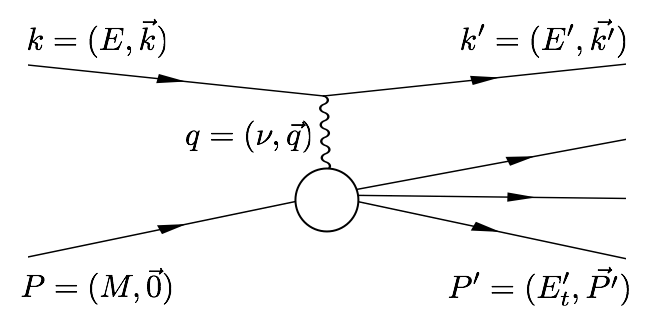
\includegraphics[width=0.6\textwidth]{figs/inclusive-scattering.png}
  \caption[Diagram for inclusive electron scattering.]{Diagram for inclusive electron scattering. \label{C2S1F1}}
\end{figure}

Two independent Lorentz invariants can be constructed from these kinematic variables. The energy transfer $\nu=(P\cdot q)/M$ and the squared four-momentum transfer $q^2=(k-k')^2$ are chosen to describe the inclusive scattering process \cite{Halzen1984}. For a space-like virtual photon, $q^2<0$, the variable $Q^2=-q^2$ is used instead of $q^2$. Since the $E$ and $E'$ are always much larger than the electron mass $m_e$ in the scattering experiments, the electron mass can be neglected. In this case, $\nu$ and $Q^2$ can be expressed as:
\begin{gather} \label{C2S1E1}
\nu = E-E', \\ \label{C2S1E2}
Q^2 = 4EE'\sin\frac{\theta}{2}.
\end{gather}
We also refer to the invariant mass of the final hadronic state:
\begin{equation} \label{C2S1E3}
W^2 = (P+q)^2 = M^2+2M\nu-Q^2.
\end{equation}
For convenience, two dimensionless scalar invariants are commonly used to replace $\nu$ and $Q^2$: the Bjorken scaling variable
\begin{equation}  \label{C2S1E4}
x = \frac{Q^2}{2P\cdot q}=\frac{Q^2}{2M\nu},
\end{equation}
and the fraction of the electron energy loss
\begin{equation} \label{C2S1E5}
y = \frac{P\cdot q}{P\cdot k}=\frac{E-E'}{E}.
\end{equation}

\section{Cross-Sections and Structure Functions}
\label{C2S2}

Consider the inclusive scattering of polarized electrons off polarized nucleons. The differential cross-section for detecting the final electron in the solid angle $\dd{\Omega}$ and in the final energy range ($E'$, $E'+\dd{E}$) in the laboratory frame can be written as \cite{Leader1996}:
\begin{equation} \label{C2S2E1}
\frac{\dd[2]{\sigma}}{\dd{\Omega}\dd{E'}} = \frac{\alpha^2}{Q^4}\frac{E'}{E}L_{\mu\nu}W^{\mu\nu},
\end{equation}
where $\alpha$ is the electromagnetic fine structure constant, $L_{\mu\nu}$ and $W^{\mu\nu}$ are the leptonic and hadronic tensor respectively. Defining the spin four-vector of the initial and final electron as $s_\mu$ and $s'_\mu$ respectively, the leptonic tensor $L_{\mu\nu}$ is calculable from QED:
\begin{equation} \label{C2S2E2}
L_{\mu\nu}(k,s;k's') = \sum_{s'}\bar{u}(k,s)\gamma_\mu u(k',s')\bar{u}(k',s')\gamma_\nu u(k,s),
\end{equation}
where $u$ is the Dirac spinor and $s_\mu=\bar{u}\gamma_\mu\gamma_5 u$. $L_{\mu\nu}$ can be split into symmetric (S) and antisymmetric (A) parts under $\mu$, $\nu$ interchange:
\begin{equation} \label{C2S2E3}
L_{\mu\nu}(k,s;k') = 2[L_{\mu\nu}^{(S)}(k;k') + iL_{\mu\nu}^{(A)}(k,s;k')],
\end{equation}
with
\begin{align} \label{C2S2E4}
& L_{\mu\nu}^{(S)}(k;k') = k_\mu k'_\nu+k'_\mu k_\nu-g_{\mu\nu}(k\cdot k'-m_e^2), \\ \label{C2S2E5}
& L_{\mu\nu}^{(A)}(k,s;k') = m_e\varepsilon_{\mu\nu\alpha\beta}s^\alpha q^\beta.
\end{align}
The convention for the Levi-Civita tensor is $\varepsilon_{0123}=+1$.

Due to the lack of knowledge of the hadronic vertex in \Cref{C2S1F1}, the hadronic tensor $W_{\mu\nu}$ is not yet calculable from first principles. Considering all possible transitions of the nucleon from the ground state $\ket{N(P)}$ to any excited state $\ket{X(P')}$, the hadronic tensor becomes \cite{Thomas2001}:
\begin{equation} \label{C2S2E6}
\begin{split}
W_{\mu\nu}(q;P,S) = \quad & \frac{1}{2M}\sum_X\mel{N_S(P)}{J_\mu(0)}{X(P')}\mel{X(P')}{J_\nu(0)}{N_S(P)} \\
& \cdot(2\pi)^3\delta^4(q+P-P'),
\end{split}
\end{equation}
where $S^\mu=\bar{u}(P)\gamma^\mu\gamma_5u(P)/2M$ is the hadron spin four-vector and $J_\mu$ is the electromagnetic current operator of the nucleon. Using the completeness relations of states $\ket{X}$, the tensor $W_{\mu\nu}$ can be expressed as:
\begin{equation} \label{C2S2E7}
W_{\mu\nu}(q;P,S) = \frac{1}{4\pi M}\int\dd[4]{\xi}e^{iq\cdot\xi}\mel{N_S(P)}{J_\mu(\xi)J_\nu(0)}{N_S(P)},
\end{equation}
where $\xi$ is the spatial four-vector.

As in \cref{C2S2E3}, the hadronic tensor can also be split into symmetric and antisymmetric parts:
\begin{equation} \label{C2S2E8}
W_{\mu\nu}(q;P,S) = W_{\mu\nu}^{(S)}(q;P) + iW_{\mu\nu}^{(A)}(q;P,S).
\end{equation}
Taking into account the gauge invariance and parity conservation of the electromagnetic interaction, the most general expressions of these terms are \cite{Anselmino1995}:
\begin{equation} \label{C2S2E9}
\begin{split}
W_{\mu\nu}^{(S)}(q;P) = \quad & W_1(\nu,Q^2)\left(\frac{q_\mu q_\nu}{q^2}-g_{\mu\nu}\right) \\
+ & \frac{W_2(\nu,Q^2)}{M^2}(P_\mu-\frac{P\cdot q}{q^2}q_\mu)(P_\nu-\frac{P\cdot q}{q^2}q_\nu),
\end{split}
\end{equation}
and
\begin{equation} \label{C2S2E10}
W_{\mu\nu}^{(A)}(q;P,S) = \varepsilon_{\mu\nu\alpha\beta}q^\alpha\left[G_1(\nu,Q^2)S^\beta+\frac{G_2(\nu,Q^2)}{M^2}(S^\beta P\cdot q-P^\beta S\cdot q)\right],
\end{equation}
where $W_{1,2}(\nu,Q^2)$ and $G_{1,2}(\nu,Q^2)$ are four response functions which describe the internal structure of the nucleon.

From \cref{C2S2E1,C2S2E3,C2S2E8}, one has:
\begin{equation} \label{C2S2E11}
\frac{\dd[2]{\sigma}}{\dd{\Omega}\dd{E'}}(k,s,P,S;k')= \frac{\alpha^2}{Q^4}\frac{E'}{E}\left[2L_{\mu\nu}^{(S)}W^{\mu\nu}_{(S)}-2L_{\mu\nu}^{(A)}W^{\mu\nu}_{(A)}\right].
\end{equation}
The two terms in the brackets can be separately studied by considering different polarizations of the initial electron and the target nucleon. For example, the first term is the usual unpolarized cross-section:
\begin{equation} \label{C2S2E12}
\frac{\dd[2]{\sigma}^{\mathrm{unp}}}{\dd{\Omega}\dd{E'}}(k,P;k') = \frac{1}{4}\sum_{s,S}\frac{\dd[2]{\sigma}}{\dd{\Omega}\dd{E'}}(k,s,P,S;k') = \frac{\alpha^2}{Q^4}\frac{E'}{E}2L_{\mu\nu}^{(S)}W^{\mu\nu}_{(S)}.
\end{equation}
In the polarized case, the difference of cross-sections with opposite target spins are given by the second term in \cref{C2S2E11}:
\begin{equation} \label{C2S2E13}
\frac{\dd[2]{\sigma}}{\dd{\Omega}\dd{E'}}(k,s,P,-S;k')-\frac{\dd[2]{\sigma}}{\dd{\Omega}\dd{E'}}(k,s,P,S;k') = \frac{\alpha^2}{Q^4}\frac{E'}{E}4L_{\mu\nu}^{(A)}W^{\mu\nu}_{(A)}.
\end{equation}

In practice, the response functions $W_{1,2}(\nu,Q^2)$ and $G_{1,2}(\nu,Q^2)$ are often replaced by four dimensionless structure functions in terms of the Bjorken variable $x$ and the squared four-momentum transfer $Q^2$:
\begin{align} \label{C2S2E14}
F_1(x,Q^2) & = MW_1(\nu,Q^2), \\  \label{C2S2E15}
F_2(x,Q^2) & = \nu W_2(\nu,Q^2), \\  \label{C2S2E16}
g_1(x,Q^2) & = M \nu G_1(\nu,Q^2), \\  \label{C2S2E17}
g_2(x,Q^2) & = \nu^2G_2(\nu,Q^2).
\end{align}
In terms of $F_{1,2}$ and  $g_{1,2}$, \cref{C2S2E9,C2S2E10} becomes
\begin{align}
W_{\mu\nu}^{(S)}(q;P) & = \frac{1}{M}\left(\frac{q_\mu q_\nu}{q^2}-g_{\mu\nu}\right)F_1(x,Q^2) \notag \\ \label{C2S2E18}
& \quad +\frac{1}{\nu M^2}(P_\mu-\frac{P\cdot q}{q^2}q_\mu)(P_\nu-\frac{P\cdot q}{q^2}q_\nu)F_2(x,Q^2), \\ \label{C2S2E19}
W_{\mu\nu}^{(A)}(q;P,S) & = \frac{1}{M\nu}\varepsilon_{\mu\nu\alpha\beta}q^\alpha\left[S^\beta g_1(x,Q^2)+(S^\beta-\frac{S\cdot q}{P\cdot q}P^\beta)g_2(x,Q^2)\right].
\end{align}

Using \cref{C2S2E12,C2S2E4,C2S2E18}, the differential cross-section for the inelastic scattering of unpolarized electron on unpolarized nucleon can be written as:
\begin{equation} \label{C2S2E20}
\frac{\dd[2]{\sigma}}{\dd{\Omega}\dd{E'}} = \sigma_{\mathrm{Mott}}\left[\frac{2}{M}F_1(x,Q^2)\tan^2\frac{\theta}{2}+\frac{1}{\nu}F_2(x,Q^2)\right],
\end{equation}
where $\sigma_{\mathrm{Mott}}$ is the cross-section for an electron scattered by a point-like heavy target, which can be expressed as:
\begin{equation} \label{C2S2E21}
\sigma_{\mathrm{Mott}} = \frac{\alpha^2\cos[2](\theta/2)}{4E^2\sin[4](\theta/2)}.
\end{equation}

For polarized electrons and target, the difference of cross-sections for scattering a polarized electron with spin $s$ on a polarized target with spin $S$ and that with spin $-S$ can be written using \cref{C2S2E13,C2S2E5,C2S2E19}:
\begin{equation} \label{C2S2E22}
\begin{split}
\frac{\dd[2]{\sigma}^{s,S}}{\dd{\Omega}\dd{E'}}-\frac{\dd[2]{\sigma}^{s,-S}}{\dd{\Omega}\dd{E'}} & = \frac{8m\alpha^2}{q^4}\frac{E'}{E}\frac{1}{M\nu}\Big\{[(q\cdot S)(q\cdot s)+Q^2(s\cdot S)]g_1(x,Q^2) \\
& \quad +\frac{Q^2}{M\nu}[(s\cdot S)(P\cdot q)-(q\cdot S)(P\cdot s)]g_2(x,Q^2)\Big\}.
\end{split}
\end{equation}

Considering the case that the electron is longitudinal polarized, while the nucleon are polarized along ($S$) or opposite ($-S$) to an arbitrary direction $\vec{S}$, the cross-section difference can be expressed in terms of $g_1$ and $g_2$ as:
\begin{equation} \label{C2S2E23}
\begin{split}
& \frac{\dd[2]{\sigma}^{\rightarrow,S}}{\dd{\Omega}\dd{E'}}-\frac{\dd[2]{\sigma}^{\rightarrow,-S}}{\dd{\Omega}\dd{E'}} = -\frac{4\alpha^2}{Q^2}\frac{E'}{E} \\
& \quad \times\frac{1}{\nu M}\left[(E\cos\alpha+E'\cos\Theta)g_1(x,Q^2)+\frac{2EE'}{\nu}(\cos\Theta-\cos\alpha)g_2(x,Q^2)\right],
\end{split}
\end{equation}
where $\alpha$ is the angle between the incident electron momentum $\vec{k}$ and the direction of the target polarization $\vec{S}$. $\Theta$ is the angle between the outgoing electron momentum $\vec{k'}$ and $\vec{S}$. If $\phi$ is the azimuthal angle between the scattering plane ($\vec{k}$, $\vec{k'}$) and the polarization plane ($\vec{k}$, $\vec{S}$), $\cos\Theta$ can be expressed as:
\begin{equation} \label{C2S2E24}
\cos\Theta = \sin\theta\sin\alpha\cos\phi+\cos\theta\cos\alpha,
\end{equation}
where $\theta$ is the scattering angle. See \Cref{C2S2F1} for the definitions of the angles $\alpha$, $\theta$ and $\phi$.

\begin{figure}[tb!]
  \centering
  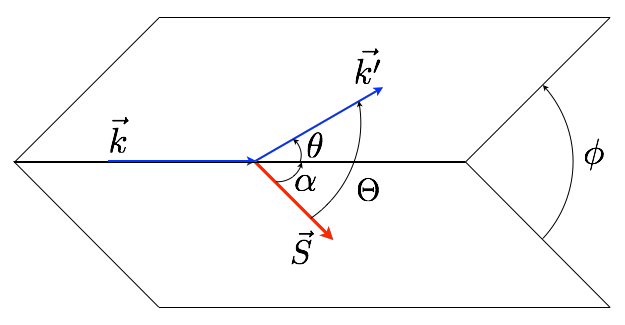
\includegraphics[width=0.5\textwidth]{figs/angles-of-polarized-scattering.png}
  \caption[Angular relations of polarized electron scattering.]{Angular relations of polarized electron scattering. \label{C2S2F1}}
\end{figure}

Therefore, one can derive the cross-section difference for some special values of $\alpha$. For the case that the target nucleons are longitudinally polarized, $\alpha=0$ and $\Theta=\theta$, the cross-section difference for the electron scattering on the nucleon polarized parallel ($\buildrel\rightarrow\over\Rightarrow$) or anti-parallel ($\buildrel\rightarrow\over\Leftarrow$) to the initial electron direction (i.e. the electron spin direction since the electron is longitudinal polarized) can be expressed as:
\begin{equation} \label{C2S2E25}
\frac{\dd[2]{\sigma}^{\buildrel\rightarrow\over\Leftarrow}}{\dd{\Omega}\dd{E'}}-\frac{\dd[2]{\sigma}^{\buildrel\rightarrow\over\Rightarrow}}{\dd{\Omega}\dd{E'}}=\frac{4\alpha^2E'}{\nu MQ^2E}\left[(E+E'\cos\theta)g_1(x,Q^2)-2Mxg_2(x,Q^2)\right].
\end{equation}
If the target nucleons are transversely polarized and the nucleon spin lies in the scattering plane, $\alpha=\pi/2$ and $\phi=0$ or $\pi$, the cross-section difference can be expressed as:
\begin{equation} \label{C2S2E26}
\frac{\dd[2]{\sigma}^{\rightarrow\Uparrow}}{\dd{\Omega}\dd{E'}}-\frac{\dd[2]{\sigma}^{\rightarrow\Downarrow}}{\dd{\Omega}\dd{E'}}=\frac{4\alpha^2E'^2}{\nu MQ^2E}\sin\theta\left[g_1(x,Q^2)+\frac{2E}{\nu}g_2(x,Q^2)\right].
\end{equation}

\section{Structure Functions in the Parton Model}
\label{C2S3}

In the last Section, the hadronic tensor $W_{\mu\nu}$ was written in term of the structure functions $F_{1,2}$ and $g_{1,2}$. One of the important feature of the structure functions is their scaling behavior in the Bjorken limit \cite{Bjorken1969}:
\begin{equation} \label{C2S3E1}
Q^2\to\infty, \text{ and } \nu\to\infty, \text{ with } x=\frac{Q^2}{2M\nu}. \text{ fixed}
\end{equation}
It turns out that to a very good approximation the structure functions are independent of $Q^2$ and can be written as $F_{1,2}(x)$ and $g_{1,2}(x)$. This phenomenon known as Bjorken scaling was first discovered at the Stanford Linear Accelerator \cite{Kendall1991}.

The parton model of Feynman \cite{Feynman1969} provides a clear explanation for the Bjorken scaling. Any object with a finite size must have a form factor which introduces some $Q^2$ dependence. Thus, the fact of Bjorken scaling implies that the nucleon must contain point-like constituents, which are named partons. Since the structure functions are Lorentz invariant, the parton model can be formulated in any frame. For convenience, the infinite momentum frame, where the nucleon is moving with momentum approaching $\infty$ along the $z$-direction, is chosen to formulate the parton model. Due to time dilatation, there is no time for interaction between the partons in this frame and the process can be viewed as the incoherent sum of elastic scattering from non-interacting partons, that is: the hadronic tensor $W_{\mu\nu}$ is given in terms of the elementary quark tensor $w_{\mu\nu}$ by \cite{Leader1996}:
\begin{equation} \label{C2S3E2}
W_{\mu\nu}(q;P,S) = \sum_{i,s}e_i^2\frac{1}{2P\cdot q}\int_0^1\frac{\dd{x'}}{x'}\delta(x'-x)n_i(x',s;S)w_{\mu\nu}(x',q,s),
\end{equation}
where the $\sum_i$ runs over quarks and antiquarks, and $n_i$ is the number density of the quark $i$ with charge $e_i$. Since quarks are point-like particles in the model, the quark tensor $w_{\mu\nu}$ is similar to the lepton tensor $L_{\mu\nu}$.

To evaluate the structure functions from \cref{C2S3E2}, four projection operators are defined as \cite{Anselmino1995}:
\begin{align} \label{C2S3E3}
P_1^{\alpha\beta} & \equiv \frac{1}{4}\left[\frac{1}{a}P^\alpha P^\beta-g^{\alpha\beta}\right], \\ \label{C2S3E4}
P_2^{\alpha\beta} & \equiv \frac{3P\cdot q}{4a}\left[\frac{1}{a}P^\alpha P^\beta-\frac{1}{3}g^{\alpha\beta}\right],
\end{align}
where $a=(P\cdot q)/2x+M^2$, and
\begin{align} \label{C2S3E5}
P_3^{\alpha\beta} & \equiv \frac{(P\cdot q)^2}{bM^2(q\cdot S)}\left[(q\cdot S)S_\lambda+q_\lambda\right]P_\eta\varepsilon^{\alpha\beta\lambda\eta}, \\ \label{C2S3E6}
P_4^{\alpha\beta} & \equiv \frac{1}{b}\left\{\left[\frac{(P\cdot q)^2}{M^2}+2(P\cdot q)x\right]S_\lambda+(q\cdot S)q_\lambda\right\}P_\eta\varepsilon^{\alpha\beta\lambda\eta},
\end{align}
where
\begin{equation} \label{C2S3E7}
b = -4M\left[\frac{(P\cdot q)^2}{M^2}+2(P\cdot q)x-(q\cdot S)^2\right].
\end{equation}
With these projectors, one has:
\begin{equation} \label{C2S3E8}
\begin{aligned}
P_1^{\alpha\beta}W_{\alpha\beta} & = F_1, & \qquad P_2^{\alpha\beta}W_{\alpha\beta} & = F_2, \\
P_3^{\alpha\beta}W_{\alpha\beta} & = g_1, & \qquad P_4^{\alpha\beta}W_{\alpha\beta} & = g_1+g_2.
\end{aligned}
\end{equation}

Applying the projection operator \cref{C2S3E3,C2S3E4,C2S3E5,C2S3E6} to \cref{C2S3E2}, one can obtain the relations between the nucleon structure functions and the parton distribution functions:
\begin{align} \label{C2S3E9}
F_1(x) & = \frac{1}{2}\sum_ie_i^2q_i(x), \\ \label{C2S3E10}
F_2(x) & = x\sum_ie_i^2q_i(x) = 2xF_1(x), \\ \label{C2S3E11}
g_1(x) & = \frac{1}{2}\sum_ie_i^2\Delta q_i(x),
\end{align}
where $q(x)=q^\uparrow(x)+q^\downarrow(x)$ is the unpolarized parton distribution function, which is the probability of finding a quark carrying the fraction $x$ of the momentum of the nucleon. $\Delta q(x)=q^\uparrow(x)-q^\downarrow(x)$ is the polarized parton distribution function, where $q^\uparrow(x)$ ($q^\downarrow(x)$) is the number density of the quark carrying the fraction $x$ of the momentum of the nucleon when it is aligned parallel (or anti-parallel) to the nucleon spin direction. \cref{C2S3E10} is a relation between $F_1$ and $F_2$ which is also known as the Callan-Gross relation \cite{Callan1969}.

The transverse polarized structure function $g_2(x)$ is zero in the naive parton model described above. However, if one allows the continent quarks to have an intrinsic transverse momentum in the nucleon, the value of $g_2$ can be non-zero.
The interpretation of $g_2(x)$ in the naive parton model is not as simple as the other structure functions \cite{Thomas2001}. It carries the information of the quark-gluon interaction inside the nucleon, which will be introduced in the next chapter.

The scaling behavior of the structure functions is only valid at the Bjorken limit as mentioned at the beginning of this section. At finite $Q^2$, the Bjorken scaling is only a good approximation since the interaction between quarks can not be ignored. QCD radiative corrections need to be included in the cross-section calculation. \Cref{C2S3F1} shows two basic processes which cannot be separated from the major process of electron scattering. In particular, the electron scattering process from a quark cannot be separated from the scattering processes with a soft gluon radiated. As the radiative effects in QED, the soft gluon radiation also gives rise to an infinite cross-section which can be renormalized if all other processes at the same order are included.

\begin{figure}[tb!]
  \centering
  \begin{subfigure}[t]{0.35\textwidth}
    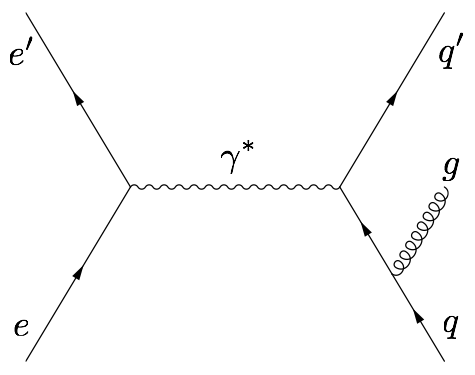
\includegraphics[width=\textwidth]{figs/gluon-radiation-a.png}
  \end{subfigure}
  \begin{subfigure}[t]{0.35\textwidth}
    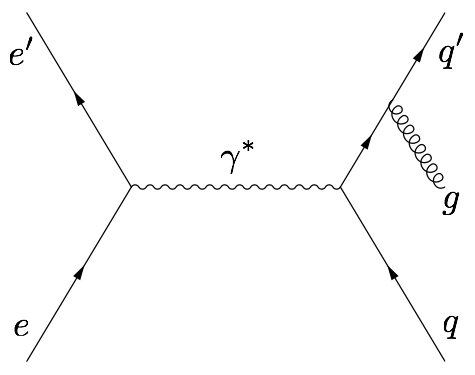
\includegraphics[width=\textwidth]{figs/gluon-radiation-b.png}
  \end{subfigure}
  \caption[Gluon radiation in electron-quark scattering.]{Radiating process which cannot be separated from the basic process of electron scattering. \label{C2S3F1}}
\end{figure}

\begin{figure}[p!]
  \centering
  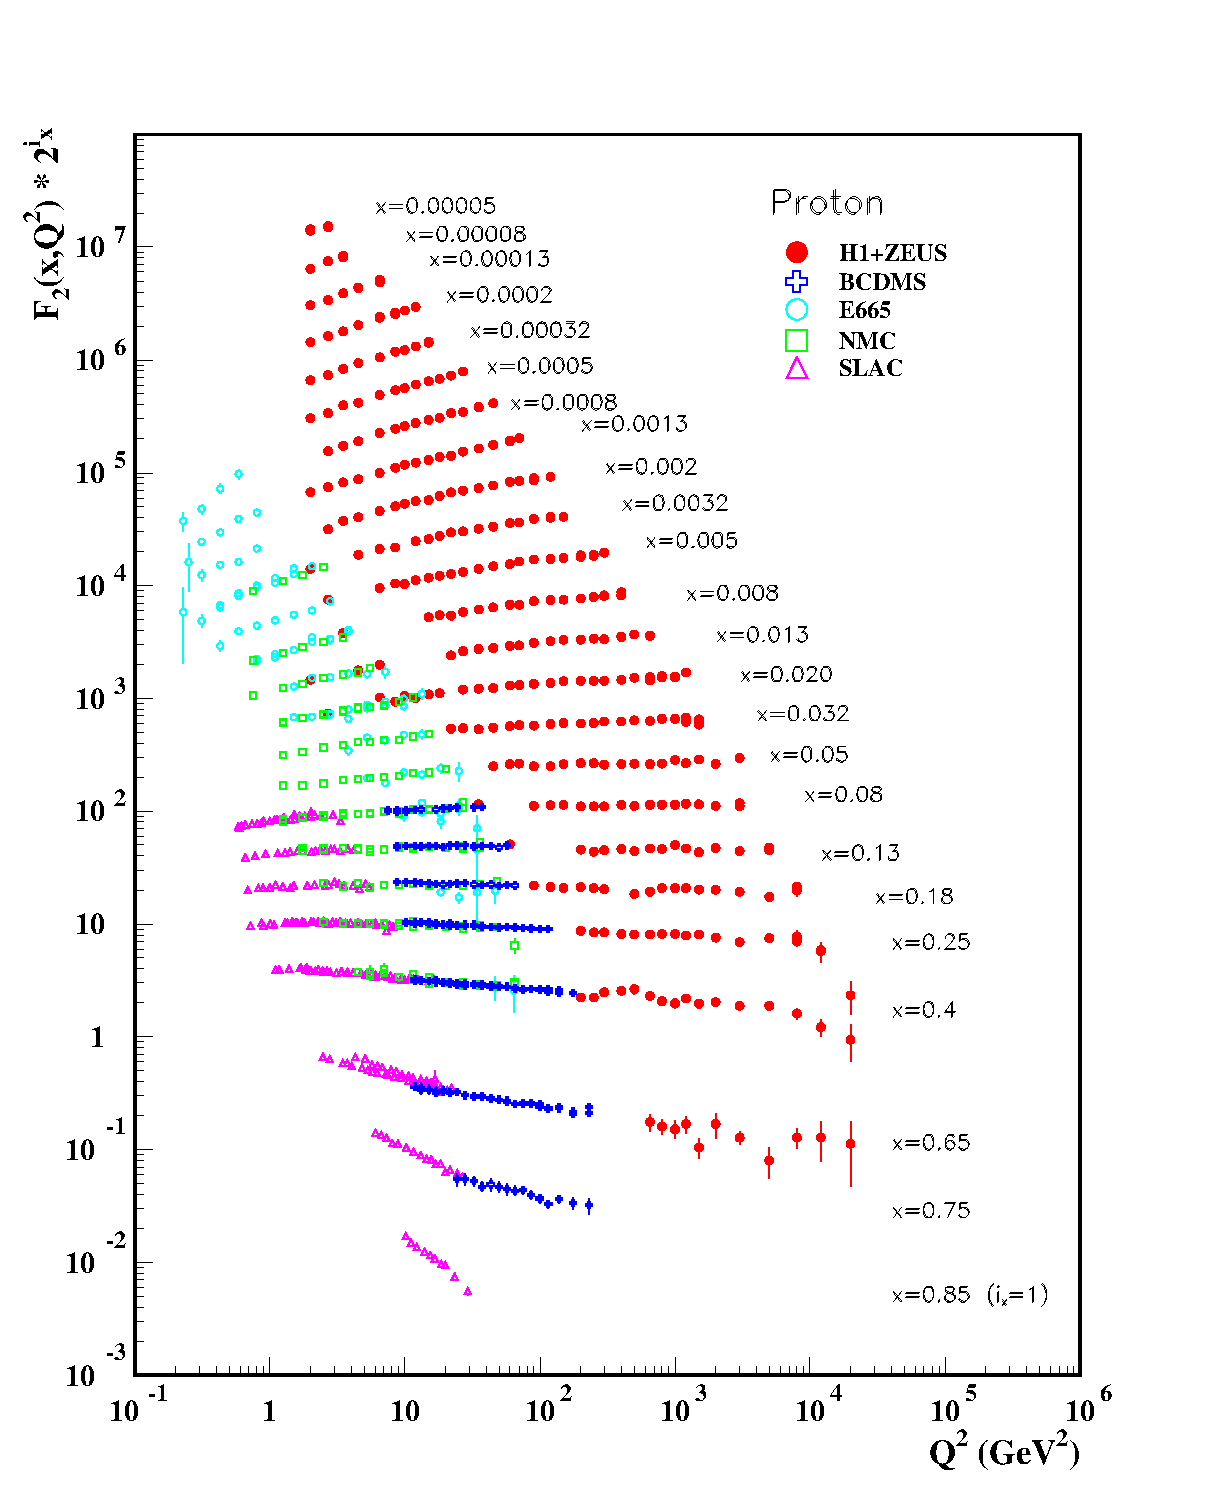
\includegraphics[width=\textwidth,trim=0 0 10mm 25mm]{figs/f2collider-logf2}
  \caption[The $Q^2$ dependence of the proton structure function $F_2^p$.]{The proton structure function $F_2^p$ measured in electromagnetic scattering of electrons and positrons off protons (collider experiments H1 and ZEUS for $Q^2\geq 2\text{ GeV}^2$) and for electrons (SLAC) and muons (BCDMS, E665, NMC) on a fixed target. The data are plotted as a function of $Q^2$ in bins of fixed $x$. For the purpose of plotting, $F_2^p$ has been multiplied by $2^{i_x}$, where $i_x$ is the number of the $x$ bin, ranging from $i_x= 1$ ($x=0.85$) to $i_x=24$ ($x=0.00005$). Plot reproduced from \cite{Olive2014}. \label{C2S3F2}}
\end{figure}

This variation of the structure functions with $Q^2$ is referred to as QCD evolution. After renormalization, the gluon radiative correction gives a logarithmic dependence to the cross-section. \Cref{C2S3F2} shows the experimental $Q^2$-dependence of the proton $F_2$ structure function for a large range of $x$ \cite{Olive2014}. By incorporating the $Q^2$-dependence into the definition of the parton distributions, the expression of structure functions can be generalized as:
\begin{align} \label{C2S3E12}
F_1(x,Q^2) & = \frac{1}{2}\sum_ie_i^2q_i(x,Q^2), \\ \label{C2S3E13}
g_1(x,Q^2) & = \frac{1}{2}\sum_ie_i^2\Delta q_i(x,Q^2).
\end{align}
Now $q(x,Q^2)\dd{x}$ should be interpreted as the probability of finding a quark in the nucleon with momentum fraction between $x$ and $x+\dd{x}$ when viewed with a resolution determined by $Q^2$. If one probes the proton at low $Q^2$, the wavelength is large ($1/\sqrt{Q^2}$) and the spatial resolution is poor. The structure functions is expected to be dominated by the valence quarks at this case. As $Q^2$ increases, more and more $q\bar{q}$ pairs and gluons can be seen since the resolution becomes better.

The QCD evolution can be calculated from perturbative QCD in the leading order. The Altarelli Parisi, or DGLAP equations developed by Gribov and Lipatov \cite{Gribov1972}, Dokshitzer \cite{Dokshitzer1977} and Altarelli and Parisi \cite{Altarelli1977} provide a method to calculate the $Q^2$-dependence of the structure functions. These equations are first-order integro-differential equations. Thus, the parton distributions can be calculated at any $Q^2$ scale where perturbative QCD applies if the distributions at some particular scale is known.

\section{Virtual Photon-absorption Cross-Sections: An Alternative Formulation}
\label{C2S4}

The previous sections revealed that the inclusive scattering process can be formulated with four structure functions. Before we go further, it is worth introducing an equivalent formulation of the inclusive scattering process in which the cross-section is parameterized in terms of four virtual photon-absorption cross-sections.

\subsection{Virtual Photon-absorption Cross-Sections}
\label{C2S4SS1}

As shown in \Cref{C2S1F1}, the inclusive scattering process is equivalent to absorption of a virtual photon on a nucleon. In the center of mass (c.m.) frame of the hadronic intermediate state, the four-momentum of the virtual photon is given by ($\omega_\gamma$, $\vec{k}_\gamma$), which can be expressed as \cite{Drechsel2004}:
\begin{equation} \label{C2S4E1}
\omega_\gamma = \frac{M\nu-Q^2}{W}, \qquad \vec{k}_\gamma = \frac{M}{W}\vec{q}.
\end{equation}
where $|\vec{q}|=\sqrt{\nu^2+Q^2}$ is the lab photon momentum. Since $\omega_\gamma$ vanishes at $\nu=Q^2/M$ and therefore is inconvenient in the context of the multipole expansion, one can define the ``equivalent photon energy'' or the virtual photon flux $K$ to replace $\omega_\gamma$ according to Hand's definition \cite{Hand1963}:
\begin{equation} \label{C2S4E2}
K = K_H = \nu(1-x) = \frac{W^2-M^2}{2M}.
\end{equation}
An alternative convention could be Gilman's definition \cite{Gilman1968}:
\begin{equation} \label{C2S4E3}
K = K_G = |\vec{q}| = \sqrt{\nu^2+Q^2}.
\end{equation}
\cref{C2S4E2,C2S4E3} reduce to $\nu$ for the real photon scattering at $Q^2=0$. However, at intermediate $Q^2$, the photon flux is strongly convention dependent.

The inclusive electron-nucleon scattering can then be parameterized in terms of a flux factor and four partial cross-sections \cite{Drechsel2001}:
\begin{equation} \label{C2S4E4}
\frac{\dd{\sigma}}{\dd{\Omega}\dd{E'}} = \Gamma_V[\sigma_T+\epsilon\sigma_L-hP_x\sqrt{2\epsilon(1-\epsilon)}\slt-hP_z\sqrt{1-\epsilon^2}\stt],
\end{equation}
where $h$ is the helicity of the longitudinally polarized electron and $P_z$ and $P_x$ denote the components of the target polarization parallel and perpendicular to the virtual photon momentum $\vec{q}$ in the scattering plane of the electron respectively. The $\epsilon$ is the photon polarization and $\Gamma_V$ is the virtual photon flux factor:
\begin{equation*}
\epsilon = \frac{1}{1+2(1+\nu^2/Q^2)\tan^2\theta/2}, \qquad \Gamma_V = \frac{\alpha}{2\pi^2}\frac{E'}{E}\frac{K}{Q^2}\frac{1}{1-\epsilon}.
\end{equation*}
The four partial cross-sections are the transverse ($\sigma_T$) and longitudinal ($\sigma_L$) cross-sections and two interference terms: the longitudinal-transverse cross-sections ($\slt$) and the transverse-transverse cross-sections ($\stt$). $\sigma_T$ and $\sigma_L$ represent the cross-sections for absorption of transverse and longitudinal virtual photons respectively. $\sigma_L$ vanishes in the $Q^2=0$ (real photon) limit since the real photon is transversely polarized. Therefore, the total photon-absorption cross-section is given by $\sigma_T$ in the real photon limit. The two spin-flip cross-sections can only be measured by double-polarization experiments.

The partial cross-sections $\sigma_T$ and $\stt$ can be expressed in terms of the helicity dependent photo-absorption cross-sections $\sigma_{1/2}$ and $\sigma_{3/2}$. The subscripts refer to the total helicity of the photon plus the target nucleon. \Cref{C2S4F1} shows the two different situations. These helicity dependent cross-sections are related to $\sigma_T$ and $\stt$ through:
\begin{equation} \label{C2S4E5}
\sigma_T = \frac{1}{2}(\sigma_{1/2}+\sigma_{3/2}), \qquad \stt = \frac{1}{2}(\sigma_{1/2}-\sigma_{3/2}).
\end{equation}

\begin{figure}[tb!]
  \centering
  \begin{subfigure}[t]{0.4\textwidth}
    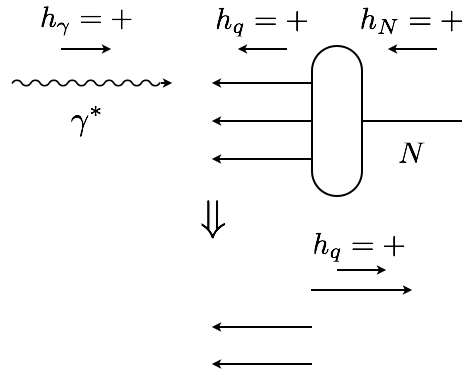
\includegraphics[width=\textwidth]{figs/photon-absorption-a.png}
    \subcaption{{}\label{C2S4F1A}}
  \end{subfigure}
  \qquad
  \qquad
  \begin{subfigure}[t]{0.4\textwidth}
    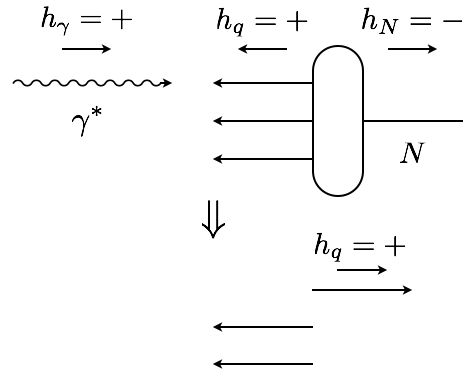
\includegraphics[width=\textwidth]{figs/photon-absorption-b.png}
    \subcaption{{}\label{C2S4F1B}}
  \end{subfigure}
  \caption[Schematic of the helicity dependent cross-sections $\sigma_{1/2}$ and $\sigma_{3/2}$.]{The helicity dependent cross-sections for a positive helicity virtual photon ($h_\gamma=+$) to be absorbed by a polarized nucleon (here $h_N=\pm$ means $h_N=\pm 1/2$): (a) $\sigma_{1/2}$ and (b) $\sigma_{3/2}$. \label{C2S4F1}}
\end{figure}

The relations between the structure functions and the photo-absorption cross-sections can be written as \cite{Thomas2001,Drechsel2003}:
\begin{align} \label{C2S4E6}
\sigma_T & = AF_1, \\ \label{C2S4E7}
\sigma_L & = A\left[\frac{(1+\gamma^2)M}{\gamma^2\nu}F_2-F_1\right], \\ \label{C2S4E8}
\stt & = A(g_1-\gamma^2g_2), \\ \label{C2S4E9}
\slt & = A\gamma(g_1+g_2),
\end{align}
where $\gamma=Q/\nu$ and $A=4\pi^2\alpha/MK$.

\subsection{Compton Scattering}
\label{C2S4SS2}

Now consider the elastic real photon scattering process $\gamma(k)+N(P)\rightarrow\gamma(k')+N(P')$. The four-momentum of the incident and scattered real photon is $k=(\nu,\vec{k})$ and $k'=(\nu',\vec{k'})$ respectively with $k^2=k'^2=0$. In the laboratory frame, the four-momentum of the nucleon is $P=(M,0)$. If we denote the scattering angle by $\theta$ in the laboratory frame, the energy and momentum conservation gives \cite{Thomas2001}:
\begin{equation} \label{C2S4E10}
\nu' = \frac{\nu}{1+\frac{\nu}{M}(1-\cos\theta)}.
\end{equation}

The polarization of the incident and scattered photons can be characterized by two linear polarization vectors $\epsilon^\mu$ and $\epsilon'^\nu$. Due to the transverse nature of real photon, we choose:
\begin{equation} \label{C2S4E11}
\begin{split}
\epsilon^\mu = (0,\vec{\epsilon}), & \quad \vec{k}\cdot\vec{\epsilon} = 0, \\
\epsilon'^\nu = (0,\vec{\epsilon'}), & \quad \vec{k'}\cdot\vec{\epsilon'} = 0.
\end{split}
\end{equation}
We can choose a coordinate system such that the $z$-axis coincides with the direction of $\vec{k}$. The polarization vector of a linearly polarized photon can be expressed as the linear combination of two unit vectors:
\begin{equation} \label{C2S4E12}
\vec{\epsilon}_x = (1,0,0), \quad \vec{\epsilon}_y = (0,1,0).
\end{equation}
The circularly polarized photons are given by:
\begin{equation} \label{C2S4E13}
\vec{\epsilon}_{\lambda=1} = \frac{1}{\sqrt{2}}(\vec{\epsilon}_x+i\vec{\epsilon}_y), \quad \vec{\epsilon}_{\lambda=-1} = \frac{1}{\sqrt{2}}(\vec{\epsilon}_x-i\vec{\epsilon}_y),
\end{equation}
with $\vec{\epsilon}^{\;\star}_{\lambda'}\cdot\vec{\epsilon}_{\lambda}=\delta_{\lambda'\lambda}$.

The differential cross-section for real Compton scattering is given by:
\begin{equation} \label{C2S4E14}
\frac{\dd{\sigma}}{\dd{\nu}} = \left(\frac{\nu'}{8\pi M\nu}\right)^2|T_{fi}|^2.
\end{equation}
Using the polarization vectors defined in \cref{C2S4E11}, the transition matrix $T_{fi}$ of real Compton scattering can be written as \cite{Thomas2001}:
\begin{equation} \label{C2S4E15}
T_{fi} = e^2\epsilon'^{\star\mu}\epsilon^\nu T_{\mu\nu}(k',P';k,P),
\end{equation}
with
\begin{equation} \label{C2S4E16}
T_{\mu\nu} = i\int\dd[4]{x}e^{ik'\cdot x}\mel{N(P')}{\mathcal{T}\{J_\mu(x)J_\nu(0)\}}{N(P)},
\end{equation}
here $\mathcal{T}$ is the time-ordering operator.

For forward scattering with $\vec{k'}=\vec{k}$, the forward Compton scattering amplitude can be expressed as \cite{Drechsel2003}:
\begin{equation} \label{C2S4E17}
T(\nu,\theta=0) = \vec{\epsilon}\,'^\star\cdot\vec{\epsilon}f(\nu)+i\vec{\sigma}\cdot(\vec{\epsilon}\,'^\star\times\vec{\epsilon}\,)g(\nu),
\end{equation}
where $\vec{\sigma}$ are the Pauli spin matrices and $f(\nu)$, $g(\nu)$ represents the spin non-flip and flip amplitudes respectively.

According to the optical theorem, the total photon absorption cross-sections is related to the imaginary part of the forward Compton scattering amplitudes by:
\begin{equation} \label{C2S4E18}
\begin{split}
\Im f(\nu) & = \frac{\nu}{8\pi}(\sigma_{1/2}(\nu)+\sigma_{3/2}(\nu)) = \frac{\nu}{4\pi}\sigma_T(\nu), \\
\Im g(\nu) & = \frac{\nu}{8\pi}(\sigma_{1/2}(\nu)-\sigma_{3/2}(\nu)) = \frac{\nu}{4\pi}\stt(\nu).
\end{split}
\end{equation}

The amplitudes $f(\nu)$ and $g(\nu)$ can be expanded in powers of $\nu$ via the low energy theorem (LET) of Low \cite{Low1954} and Gell-Mann and Goldberger \cite{Gellmann1954b}:
\begin{align} \label{C2S4E19}
f(\nu) & = -\frac{Z^2e^2}{4\pi M}+(\alpha+\beta)\nu^2+\mathcal{O}(\nu^4), \\ \label{C2S4E20}
g(\nu) & = -\frac{\kappa^2e^2}{8\pi M^2}\nu+\gamma_0\nu^3+\mathcal{O}(\nu^5),
\end{align}
where $Z$ is the charge in the unit of elementary charge, and $\kappa$ is the anomalous magnetic moment in the unit of nuclear magneton. The leading term of the spin non-flip amplitude gives the classical Thomson scattering result. The $\mathcal{O}(\nu^2)$ term contains information of the internal structure and appears as the sum of the electric and magnetic dipole polarizabilities $\alpha$ and $\beta$. The $\mathcal{O}(\nu^3)$ term of the spin flip amplitude is related to the forward spin polarizability $\gamma_0$ with information of the spin structure.

By use of the optical theorem, the Kramers-Kronig dispersion relations can be derived for $f(\nu)$ and $g(\nu)$, which gives:
\begin{align} \label{C2S4E21}
\Re f(\nu) & = f(0)+\frac{\nu^2}{2\pi^2}\pv{\int_{\nu_0}^\infty\dd{\nu'}\frac{\sigma_T(\nu')}{\nu'^2-\nu^2}}, \\ \label{C2S4E22}
\Re g(\nu) & = \frac{\nu}{4\pi^2}\pv{\int_{\nu_0}^\infty\dd{\nu'}\nu'\frac{\sigma_{1/2}(\nu')-\sigma_{3/2}(\nu')}{\nu'^2-\nu^2}},
\end{align}
where $\pv$ means the principal value of the integral. $\nu_0$ is introduced to ensure that the integral converges. Thus, the two integrals can be expand as a Taylor series in $\nu$:
\begin{align} \label{C2S4E23}
\Re f(\nu) & = f(0)+\sum_{n=1}\left(\frac{1}{2\pi^2}\int_{\nu_0}^\infty\dd{\nu'}\frac{\sigma_T(\nu')}{\nu'^{2n}}\right)\nu^{2n}, \\ \label{C2S4E24}
\Re g(\nu) & = \sum_{n=1}\left(\frac{1}{4\pi^2}\int_{\nu_0}^\infty\dd{\nu'}\frac{\sigma_{1/2}(\nu')-\sigma_{3/2}(\nu')}{\nu'^{2n-1}}\right)\nu^{2n-1}.
\end{align}

By comparing \cref{C2S4E23,C2S4E24} with \cref{C2S4E19,C2S4E20}, we can obtain Baldin's sum rule \cite{Baldin1960,Lapidus1963} from the $\mathcal{O}(\nu^2)$ term of spin non-flip amplitude $f(\nu)$:
\begin{equation} \label{C2S4E25}
\alpha+\beta = \frac{1}{2\pi^2}\int_{\nu_0}^\infty\dd{\nu'}\frac{\sigma_T(\nu')}{\nu'^{2}}.
\end{equation}
From the leading term of the spin flip amplitude $g(\nu)$, we can obtain the Gerasimov-Drell-Hearn (GDH) sum rule \cite{Gerasimov1966,Drell1966}:
\begin{equation} \label{C2S4E26}
-2\pi^2\alpha\frac{\kappa^2}{M^2} = \int_{\nu_0}^\infty\dd{\nu'}\frac{\sigma_{1/2}(\nu')-\sigma_{3/2}(\nu')}{\nu'}\equiv I,
\end{equation}
where $\alpha=e^2/4\pi$ is the fine structure constant. And we can also obtain a relation for the forward spin polarizability \cite{Gellmann1954a,Gellmann1954b}:
\begin{equation} \label{C2S4E27}
\gamma_0 = \frac{1}{4\pi^2}\int_{\nu_0}^\infty\dd{\nu'}\frac{\sigma_{1/2}(\nu')-\sigma_{3/2}(\nu')}{\nu'^3}.
\end{equation}

The above discussion could be generalized if we treat the real photon as virtual by replacing $k$ with $q$ and assume $q^2\neq 0$. This is known as the double virtual Compton scattering (VVCS). Comparing \cref{C2S4E16} with \cref{C2S2E7}, we notice that the difference between $T_{\mu\nu}$ and the hadronic tensor $W_{\mu\nu}$ is the time ordering operator $\mathcal{T}$ of the electromagnetic currents. Actually $W_{\mu\nu}$ is related to the forward virtual Compton tensor $T_{\mu\nu}$ by \cite{Thomas2001}:
\begin{equation} \label{C2S4E190}
W_{\mu\nu}(q,P) = \frac{1}{2\pi M}\Im T_{\mu\nu}(q,P;q,P).
\end{equation}
This relation implies that the components of the hadronic tensor, e.g., the structure functions, are related to the forward double VVCS amplitudes by the Kramers-Kronig dispersion relations. We will continue the discussion of these relations in \Cref{C4}.

%%%%%%%%%%%%%%%%%%%%%%%%%%%%%%%%%%%%%%%%%%%%%%%%%%%%%%%%%%%%%%%%%%%%%%
% -*-latex-*-

% -*-latex-*-

\chapter{Theoretical Methods}
\label{C3}

The internal structure of the nucleon can be parameterized by unpolarized and polarized structure functions as described in \Cref{C2}. In this chapter, some of the most common theoretical methods to calculate the $Q^2$ evolution of the structure functions will be discussed. We will give special emphasis to the chiral perturbation theory which is expected to be applicable in the low $Q^2$, the region covered in experiment E08-027.

\section{Chiral Perturbation Theory}
\label{C3S1}

\subsection{Chiral Symmetry}
\label{C3S1SS1}

QCD is a type of quantum field theory called a non-abelian gauge theory of colored quarks and gluons. The complete QCD Lagrangian is \cite{Marciano1978}:
\begin{equation} \label{C3S1E1}
\mathcal{L}_{\mathrm{QCD}} = \sum_f\bar{q}_f(i\slashed{D}-m_f)q_f-\frac{1}{4}\mathcal{G}_{\mu\nu}^\alpha\mathcal{G}_\alpha^{\mu\nu},
\end{equation}
where $\mathcal{G}$ is the field strength tensor and $q$ is the quark spinor. The summation is taken over all six quark flavors.

One particular important concept in QCD is asymptotic freedom, which refers to the fact that the coupling strength decreases for increasing momentum transfer $Q^2$. Asymptotic freedom allows a perturbative approach at high energies for QCD by expanding in powers of the strong interaction coupling constant $\alpha_s(Q^2)$. However, for low energy interactions ($Q^2 <$ 1 GeV${}^2$), the coupling constant $\alpha_s(Q^2)$ is of order one, which makes the expansion approach no longer useful.

The masses of the three light quarks $u$, $d$ and $s$ are small compared to typical masses of light hadrons, like the $\rho$ meson (770 MeV) or the proton (938 MeV). For a massless fermion, the chirality or handedness is identical to the particle's helicity $h = \vec{\sigma}\cdot\vec{p}/|\vec{p}|$, where $\vec{\sigma}$ are the Pauli spin matrices and $\vec{p}$ is the particle's momentum. In the limit where the light quark masses vanish, the left-handed and right-handed quark fields are decoupled from each other in the QCD Lagrangian. We could introduce the left and right handed quark fields:
\begin{equation}\label{C3S1E2}
q_{L,R} = \frac{1}{2}(1\mp\gamma_5)q.
\end{equation}
and rewrite the QCD Lagrangian as \cite{Scherer2003}:
\begin{equation} \label{C3S1E3}
\mathcal{L}_{\mathrm{QCD}}^0 = \sum_{f=u,d,s}(\bar{q}_{R,f}i\slashed{D}q_{R,f}+\bar{q}_{L,f}i\slashed{D}q_{L,f})-\frac{1}{4}\mathcal{G}_{\mu\nu}^\alpha\mathcal{G}_\alpha^{\mu\nu}.
\end{equation}
The Lagrangian $\mathcal{L}_{\mathrm{QCD}}^0$ exhibits a global $\mathrm{U}(3)_L\times\mathrm{U}(3)_R$ symmetry, which is referred as chiral symmetry.

The chiral symmetry can be decomposed to a $\mathrm{SU}(3)_L\times\mathrm{SU}(3)_R\times\mathrm{U}(1)_V$ symmetry \cite{Scherer2003}. Here the $\mathrm{U}(1)_V$ symmetry is connected to baryon number conservation, where quarks and antiquarks are assigned the baryon numbers $B=1/3$ and $B=-1/3$ respectively. Mesons and baryons can be distinguished with their baryon numbers $B=0$ or $B=1$.

On the other side, although the theory admits the $\mathrm{SU}(3)_L\times\mathrm{SU}(3)_R$ symmetry, the ground state of QCD does not have the full symmetry. Consider the linear combinations of the 16 generators of the group $G=\mathrm{SU}(3)_L\times\mathrm{SU}(3)_R$, $Q_V^a=Q_R^a+Q_L^a$ and $Q_A^a=Q_R^a-Q_L^a$, $a=1,\cdots,8$, the generators $Q_V^a$ form a Lie algebra corresponding to a $\mathrm{SU}(3)_V$ subgroup $H$ of the $G$. In the chiral limit, the ground state is necessarily invariant under $H$ \cite{Vafa1984}, i.e., the eight generators $Q_V^a$ annihilate the ground state. However, if we apply $Q_A^a$ to an arbitrary state of a given multiplet with well-defined parity, we would obtain a degenerate state of opposite parity since the axial generators $Q_A^a$ have negative parity \cite{Scherer2003}. This assumes that hadrons should have a partner of the same mass but with opposite parity. Such a parity doubling is not observed in the real hadron spectrum, which means that the ground state is not invariant under the full symmetry group $G$, i.e., $Q_A^a$ do not annihilate the ground state. In other words, the chiral symmetry is spontaneously broken to the flavor group $\mathrm{SU}(3)_V$.

Goldstone's theorem requires that each generator which does not annihilate the ground state is associated with a Goldstone boson \cite{Goldstone1961, Goldstone1962}. Thus, the eight generators $Q_A^a$ imply the existence of eight massless Goldstone bosons with negative parity and baryon number zero which transform as an octet under $\mathrm{SU}(3)_V$. In nature, the eight lightest hadrons, including the pions ($\pi^\pm, \pi^0$), the kaons ($K^\pm, K^0, \bar{K}^0$) and the eta ($\eta$), compose an octet which qualifies for these Goldstone bosons. The mass of these bosons are interpreted as a result of the explicitly symmetry breaking due to the non-zero quark mass.

\subsection{Chiral Effective Field Theory}
\label{C3S1SS2}

At low-energy limit, it is impractical to directly deal with quarks and gluons since the relevant degrees of freedom in QCD at low-energy region are composite hadrons. An effective field theory is constructed to approximate the QCD in the low-energy limit which still reproduces the basic QCD symmetries and spontaneous symmetry breaking patterns.

The basic idea of an effective field theory is to treat the active, light particles as collective degrees of freedom, while the heavy particles as frozen and static sources \cite{Thomas2001}. An effective Lagrangian $\mathcal{L}_{\mathrm{eff}}$ is constructed to describe the dynamics which incorporates all symmetries of the underlying fundamental theory.

Thus, the QCD Lagrangian \cref{C3S1E1} is split into a symmetric part, $\mathcal{L}_{\mathrm{QCD}}^0$, and a symmetry breaking part $\mathcal{L}'_{\mathrm{QCD}}$ to construct this effective Lagrangian:
\begin{equation} \label{C3S1E4}
\mathcal{L}^{\mathrm{eff}}_{\mathrm{QCD}} = \mathcal{L}_{\mathrm{QCD}}^0+\mathcal{L}'_{\mathrm{QCD}},
\end{equation}
where
\begin{equation} \label{C3S1E5}
\mathcal{L}'_{\mathrm{QCD}} = -\sum_f\bar{q}_fm_fq_f
\end{equation}
is considered as a perturbation to the $\mathcal{L}_{\mathrm{QCD}}^0$.

The effective Lagrangian should be able to represent the same low-energy expansion as QCD itself. Any matrix element or scattering amplitude derived from this effective Lagrangian is organized as a low-energy expansion in powers of energies and momenta (generically denoted as $p$) of the interacting particles. Although the symmetry breaking mass term can be treated perturbatively, the convergence radius is often quite limited. However, many rigorous statements can still be made within the limit. This framework for the expansion of the effective field theory is called chiral perturbation theory ($\chi$PT) \cite{Weinberg1979}.

\subsection{Chiral Perturbative Theory for Baryons}
\label{C3S1SS3}

Chiral Perturbation Theory provides a systematic method to discuss the interaction of Goldstone bosons with each other and with the external fields, which has been discussed in many theoretical works such as \cite{Gasser1984,Gasser1985}. The baryons have also been included into the scheme as well \cite{Bernard1992}. Consider the transition matrix elements with only a single baryon in the initial and final states, we can describe many static properties such as masses or magnetic moments, form factors as well as some more complicated processes, such as pion-nucleon scattering, Compton scattering, pion photo-production etc with the help of the $\chi$PT. However, the presence of the baryons creates a complication. The low-energy expansion corresponds to an expansion in pion loops. The baryon mass does not vanish in the chiral limit and is comparable to the chiral scale $\Lambda_\chi\simeq 1$GeV, and thus only baryon three-momenta can be considered small \cite{Bernard1993}. This implies that there is no guarantee that the small-momentum expansion is exact one-to-one corresponding to the one-loop graphs. Theorists have considered two main approaches to deal with this complication: Heavy Baryon $\chi$PT (HB$\chi$PT) \cite{Jenkins1991a,Jenkins1991b} and Relativistic Baryon $\chi$PT (RB$\chi$PT) \cite{Ellis2003}.

\begin{description}
\item[Heavey Baryon $\chi$PT :] \hfill \\
The baryons are considered as very heavy in the HB$\chi$PT approach. This allows for a consistent power counting scheme as an expansion in the inverse powers of the baryon mass. The troublesome baryon mass term can be eliminated in this case. However the expansion in the ratio of pion to nucleon masses $m_\pi/M_N$ is not expected to converge very fast \cite{Bernard1993}.
\item[Relativistic Baryon $\chi$PT :] \hfill \\
The heavy baryon $\chi$PT suffers from a deficiency that the standard low energy expansion in powers of meson momenta and light quark masses in general only converges in part of the low energy region. The problem is generated by a set of higher order graphs involving insertions in nucleon lines \cite{Becher1999}. The non-relativistic expansion in HB$\chi$PT causes the problem and it does not occur in the relativistic formulation of the effective theory. This relativistically invariant formulation can extract the infrared singularities of the various one loop graphs occurring in the $\chi$PT series. This procedure can be viewed as a novel method of regularization, where any dimensionally regularized one-loop integral can be split into an infrared singular and a regular part depending on a particular choice of Feynman parameterization. The low-energy constants absorb the contribution from the regular part while non-trivial results are obtained from the chiral expansion of the infrared part. The result agrees with the one obtained with HB$\chi$PT if the chiral expansion of the one-loop integrals converge.
\end{description}

Both HB$\chi$PT and RB$\chi$PT have been used to study the spin-dependent structure functions and their moments \cite{Ji2000,Bernard2002,Kao2003,Bernard2003}. The theoretical effects in these works are limited to the two flavor case of the $u$ and $d$ quarks. Typically the $Q^2$-dependence of the Compton amplitudes is studied in the chiral limit, which can be connected to the spin structure functions via Kramers-Kronig dispersion relations as mentioned in \cref{C2S4}.

One more thing need to be mentioned is the contribution from the resonances. The resonances are expected to have significant contributions to the Compton amplitudes, especially from the $\Delta(1232)$ resonance. Ideally one would like to include the contribution from the $\Delta$ as a dynamical degree of freedom in the effective Lagrangian, however, an effective field theory formulation for the relativistic pion-nucleon-delta system does not exist. Thus, the contribution from $\Delta$ can only be done systematically in the heavy baryon scheme treating the nucleon-delta mass splitting as an additional small parameter \cite{Hemmert1998}. The $\Delta$ contribution is estimated by calculating relativistic Born graphs, which are dependent on a few experimental parameters that are not well-known. Another important resonance contribution which is less pronounced is due to the vector mesons \cite{Bernard2003}. Ref. \cite{Kubis2001} discusses the procedure to include the degrees of freedom of the vector mesons.

\section{Operator Product Expansion}
\label{C3S2}

The Operator Product Expansion (OPE) was originally introduced by Wilson in 1969 as an attempt to provide direct QCD predictions for the moments of the structure functions via sum rules \cite{Wilson1969}. The method is model-independent and the main results depend only on some very general results from Quantum Field Theory.

As mentioned in \Cref{C2S4SS2}, the hadronic tensor $W_{\mu\nu}$ of the inclusive electron-nucleon scattering is related to the forward virtual Compton tensor $T_{\mu\nu}$. At Bjorken limit, where the $Q^2$ and $p\cdot q$ are both large - typically greater than 2 GeV${}^2$, the Fourier transform in \cref{C2S4E16} is dominated by the behavior as $x^2\rightarrow 0$. The OPE is the ideal tool to deal such problems \cite{Thomas2001}.

The OPE allows the evaluation of products of operators by separating the perturbative part of the product from the non-perturbative part. For example, the product of the two operators $\mathcal{O}_a(x)\mathcal{O}_b(0)$ can be expressed as a sum over local operators in the limit of $x\rightarrow 0$ \cite{Manohar1992}:
\begin{equation} \label{C3S2E1}
\mathcal{O}_a(x)\mathcal{O}_b(0) = \sum_iC_{ab,i}(x)\mathcal{O}_i(0),
\end{equation}
where $C_{ab}$ are the Wilson coefficient functions. Because fo the asymptotic freedom feature of QCD, the coupling constant is small at short distance. Thus the Wilson coefficient functions can be calculated perturbatively in the limit of $x\rightarrow 0$.

In practice, the momentum space version of the operator product is more commonly used:
\begin{equation} \label{C3S2E2}
\int\dd[4]x e^{iq\cdot x}\mathcal{O}_a(x)\mathcal{O}_b(0).
\end{equation}
The limit $x\rightarrow 0$ forces $q\rightarrow\infty$ in the Fourier transform of the Operator Product Expansion of \cref{C3S2E1}, which can be expressed in terms of the coefficient functions that depend on $q$:
\begin{equation} \label{C3S2E3}
\lim_{q\rightarrow\infty}\int\dd[4]x e^{iq\cdot x}\mathcal{O}_a(x)\mathcal{O}_b(0) = \sum_iC_{ab,i}(q)\mathcal{O}_i(0).
\end{equation}
This expansion will be valid when $q$ is much larger than the typical hadronic mass scale $\Lambda_{\mathrm{QCD}}$.

The local operators used in OPE are quark and gluon operators with arbitrary dimension $d$ and spin $n$. With this notation, an operator with dimension $d$ and spin $n$ can be written as:
\begin{equation} \label{C3S2E4}
\mathcal{O}_{n,d}^{\mu_1\cdots\mu_n},
\end{equation}
where $\mathcal{O}$ is symmetric and traceless in $\mu_1\cdots\mu_n$. The matrix elements of $\mathcal{O}$ of a hadron are proportional to
\begin{equation} \label{C3S2E5}
\frac{\mathcal{S}[p^{\mu_1}\cdots p^{\mu_n}]}{M^{2+n-d}}
\end{equation}
for a vector operator, and to
\begin{equation} \label{C3S2E6}
\frac{\mathcal{S}[s^{\mu_1}p^{\mu_2}\cdots p^{\mu_n}]}{M^{2+n-d}}
\end{equation}
for an axial operator. Here $\mathcal{S}$ symmetries the Lorentz indices. The power of $M$ is decided by dimensional analysis. A detailed dimensional analysis gives that the contribution of the operator $\mathcal{O}$ to $W_{\mu\nu}L^{\mu\nu}$ is of order \cite{Manohar1992}:
\begin{equation} \label{C3S2E7}
x^{-n}\left(\frac{M}{Q}\right)^{\tau-2},
\end{equation}
where $\tau\equiv d-n$ is defined as the ``twist''. At large $Q^2$, the most important operator in the OPE are those with the twist-2, since higher twists are suppressed by increasing powers of $M/Q$. Thus higher twist contributions are expected to be more important for low $Q^2$. The reliable parts of the parton model can be mapped onto an OPE analysis in which the leading twist is related to the amplitude for scattering off asymptotically free quarks and the higher twists arise from the quark-gluon interaction and the quark mass effects.

\subsection{\texorpdfstring{Operator Product Expansion Analysis of $g_2$}{Operator Product Expansion Analysis of g2}}

When we discussed the structure functions in the parton model in \cref{C2S3}, we claimed that the $g_2$ structure function does not have a simple interpretation in the naive parton model. The most reliable method to explore the $g_2$ structure function is OPE. Light quark mass effects are suppressed by $m/Q$ in $F_1$ or $g_1$ but they are important in $g_2$ where they enter as $\order{m/\Lambda_{\mathrm{QCD}}}$ \cite{Jaffe1991}.

In analogy to the hadron tensor, the forward virtual Compton scattering amplitude $T_{\mu\nu}$ in \cref{C2S4E16} can be decomposed to \cite{Jaffe1990}:
\begin{align} \label{C3S2E8}
& T_{\mu\nu}(q;P,S) = T_{\mu\nu}^{(S)}(q;P) + iT_{\mu\nu}^{(A)}(q;P,S), \\ \label{C3S2E9}
& T_{\mu\nu}^{(S)}(q;P) = -g_{\mu\nu}T_1(\nu,Q^2)+\frac{P_\mu P_\nu}{M^2}T_2(\nu,Q^2)+q^\mu\;\mathrm{or}\; q^\nu\;\mathrm{terms}, \\ \label{C3S2E10}
& T_{\mu\nu}^{(A)}(q;P,S) = \frac{\varepsilon_{\mu\nu\alpha\beta}q^\alpha S^\beta}{M^2}A_1(\nu,Q^2)+\frac{\varepsilon_{\mu\nu\alpha\beta}q^\alpha(\nu S^\beta-q\cdot SP^\beta)}{M^4}A_2(\nu,Q^2).
\end{align}

From \cref{C2S4E19}, the relation between $T_{\mu\nu}$ and the hadronic tensor is $W_{\mu\nu}=T_{\mu\nu}/2\pi M$. Thus, by comparing the imaginary part of $T_{\mu\nu}$ and the hadronic tensor, we can get:
\begin{equation} \label{C3S2E11}
g_1(x,Q^2) = \frac{\nu}{2\pi M^2}\Im A_1(\nu,Q^2), \quad g_2(x,Q^2) = \frac{\nu^2}{2\pi M^4}\Im A_2(\nu,Q^2).
\end{equation}
We could define
\begin{equation} \label{C3S2E12}
\alpha_1(x,Q^2) = \frac{\nu}{M^2}A_1(\nu,Q^2), \quad \alpha_2(x,Q^2) = \frac{\nu^2}{M^4}A_2(\nu,Q^2).
\end{equation}
for convenience.
The Kramers-Kronig dispersion relations of $\alpha_1(x,Q^2)$ and $\alpha_1(x,Q^2)$ can be written as \cite{Jaffe1990}:
\begin{equation} \label{C3S2E13}
\begin{split}
\alpha_1(\omega,Q^2) & = \frac{2\omega}{\pi}\int_1^\infty\frac{\dd{\omega'}}{\omega'^2-\omega^2}\Im\alpha_1(\omega',Q^2), \\
\alpha_2(\omega,Q^2) & = \frac{2\omega^3}{\pi}\int_1^\infty\frac{\dd{\omega'}}{\omega'^2(\omega'^2-\omega^2)}\Im\alpha_2(\omega',Q^2),
\end{split}
\end{equation}
where $\omega=1/x$. Replacing $\alpha_{1,2}$ in \cref{C3S2E13} with $g_{1,2}$ and expanding the right side in Taylor series gives the dispersion relations between $\alpha_{1,2}$ and $g_{1,2}$:
\begin{equation} \label{C3S2E14}
\begin{split}
\alpha_1(x,Q^2) & = \frac{4}{x}\sum_{n=0,2,4,\dots}\left(\frac{1}{x^{n}}\right)\int_0^1\dd{y}y^ng_1(y,Q^2), \\
\alpha_2(x,Q^2) & = \frac{4}{x^3}\sum_{n=0,2,4,\dots}\left(\frac{1}{x^{n}}\right)\int_0^1\dd{y}y^{n+2}g_2(y,Q^2).
\end{split}
\end{equation}

$T_{\mu\nu}$ could also be calculated via Operator Product Expansion. The calculation result gives us the expressions for the $\alpha_1(x,Q^2)$ and $\alpha_1(x,Q^2)$ as a series of $1/x$ \cite{Jaffe1990}:
\begin{align} \label{C3S2E15}
\alpha_1(x,Q^2)+\alpha_2(x,Q^2) & = \sum_{n=0,2,4,\dots}\frac{a_n+nd_n}{n+1}\frac{1}{x^{n+1}}, \\ \label{C3S2E16}
\alpha_2(x,Q^2) & = \sum_{n=2,4,\dots}\frac{n(d_n-a_n)}{n+1}\frac{1}{x^{n+1}},
\end{align}
where $a_n$ are the twist-2 and $d_n$ are the twist-3 matrix elements of the quark and gluon operators. By comparing \cref{C3S2E15,C3S2E16} with \cref{C3S2E14}, we can get an infinite set of moment sum rules for the structure function $g_1$ and $g_2$:
\begin{align} \label{C3S2E17}
\int_0^1\dd{x}x^ng_1(x,Q^2) & = \frac{1}{4}a_n, \quad n = 0,2,4,\dots, \\ \label{C3S2E18}
\int_0^1\dd{x}x^ng_2(x,Q^2) & = \frac{1}{4}\frac{n}{n+1}(d_n-a_n), \quad n = 2,4,\dots.
\end{align}
The symmetry of the system under charge conjugation selects only even moments out in the above relations.

\cref{C3S2E17} connects $g_1$ with the twist-2 matrix element $a_n$. If we replace the $a_n$ with the corresponding moments of $g_1$, the leading twist terms cancel, and we get:
\begin{equation} \label{C3S2E19}
\int_0^1\dd{x}x^{n-1}\left(g_1(x,Q^2)+\frac{n}{n-1}g_2(x,Q^2)\right) = \frac{1}{4}d_{n-1}, \quad n \geq 3.
\end{equation}
If we only consider the leading twist effect and set the twist-3 $d_n$ terms to be 0, we can get:
\begin{equation} \label{C3S2E20}
\int_0^1\dd{x}x^{n-1}[g_1(x,Q^2)+g_2(x,Q^2)] = \int_0^1\dd{x}x^{n-1}\frac{1}{n}g_1(x,Q^2).
\end{equation}
Notice that the left hand side and the right hand side are both in the form of Mellin Transform. Using the convolution property of integral transforms and the fact that $1/n$ is the Mellin transform of unity \cite{Barone2003}, \cref{C3S2E20} can be inverted as:
\begin{equation} \label{C3S2E21}
g_1(x,Q^2)+g_2(x,Q^2) = \int_x^1\frac{\dd{y}}{y}g_1(y,Q^2).
\end{equation}
This relation is referred as the Wandzura-Wilczek relation \cite{Wandzura1977}:
\begin{equation} \label{C3S2E22}
\gtww(x,Q^2) = -g_1(x,Q^2)+\int_x^1\frac{\dd{y}}{y}g_1(y,Q^2),
\end{equation}
which shows that the leading twist part of $g_2$ is determined completely by $g_1$ and can be interpreted by the parton model.

With the Wandzura-Wilczek relation, the $g_2$ structure function can be separated into leading and higher-twist components, which can be expressed as:
\begin{equation} \label{C3S2E23}
g_2(x,Q^2) = \gtww(x,Q^2)+\bar{g}_2(x,Q^2),
\end{equation}
where
\begin{equation} \label{C3S2E24}
\int_0^1\dd{x}x^n\bar{g}_2(x,Q^2) = \frac{n}{4(n+1)}d_n, \quad n = 2,4,\dots.
\end{equation}

The higher-twist part $\bar{g}_2$ can also be separated as \cite{Slifer2004}:
\begin{equation} \label{C3S2E25}
g_2(x,Q^2) = -\int_x^1\pdv{y}\left[\frac{m_q}{M}h_T(y,Q^2)+\zeta(y,Q^2)\right]\frac{\dd{y}}{y}.
\end{equation}
There are three contributions to the structure function $g_2$ \cite{G2P}:
\begin{enumerate}
\item $\gtww$: The leading twist-2 term, which depends only on $g_1$;
\item $h_T$: Arises from the quark transverse polarization distribution. Also twist-2, this term is suppressed by the smallness of the quark mass;
\item $\zeta$: The twist-3 part which arises from quark-gluon interactions.
\end{enumerate}

The $gtww$ defined by the Wandzura-Wilczek relation is not a good approximation to $g_2$ at low $Q^2$ since the higher twist contribution can not be ignored. At typical Jefferson Lab kinematics, $g_2$ strongly deviates from its leading twist behavior which gives $g_2$ a unique sensitivity to higher twist, i.e. interaction-dependent effects in QCD \cite{Jaffe1990}.

%%%%%%%%%%%%%%%%%%%%%%%%%%%%%%%%%%%%%%%%%%%%%%%%%%%%%%%%%%%%%%%%%%%%%%
% -*-latex-*-

% -*-latex-*-

\chapter{Physics Motivation}
\label{C4}

In previous chapters, we have discussed the unpolarized and polarized structure functions and their relations to the parton model. These structure functions have been extracted over a wide kinematic range during the past 40 years. However, data on the spin structure function $g_2$ at low energy is still lacking. Jefferson Lab Experiment E08-027 will provide precise $g_2$ data for the proton in the resonance region and extract the generalized longitudinal-transverse polarizability $\dlt$. $\dlt$ is expected to be a good test for the Chiral Perturbation Theory, as mentioned in \Cref{C3S1}. In addition, the $g_2$ data in the low $Q^2$ region could be used to provide a test of the Burkhardt-Cottingham (BC) sum rule. In this chapter, we will first give an overview of the previous experiments of the structure function measurement. The generalized longitudinal-transverse polarizability $\dlt$ and the BC sum rule will be discussed as the major motivation of experiment E08-027. The low $Q^2$ $g_2$ data will also help to improve the precision of the hyperfine structure calculation of hydrogen, which will also be discussed in this chapter.

\section{\texorpdfstring{Existing $g_2$ Data}{Existing g2 Data}}
\label{C4S1}

In \Cref{C2S2}, the relations between the spin structure functions and the cross-sections have been give as \cref{C2S2E25,C2S2E26}. To extract the spin structure function $g_1$ and $g_2$, one natural way is to measure the cross-section differences, which are defined as:
\begin{align} \label{C4S1E1}
\Delta\sigma_{\parallel} & = \dd{\sigma}^{\buildrel\rightarrow\over\Leftarrow}-\dd{\sigma}^{\buildrel\rightarrow\over\Rightarrow}, \\ \label{C4S1E2}
\Delta\sigma_{\perp} & = \dd{\sigma}^{\rightarrow\Uparrow}-\dd{\sigma}^{\rightarrow\Downarrow},
\end{align}
here the arrows indicate the polarization of the electrons and the target, $\buildrel\rightarrow\over\Leftarrow$ and $\buildrel\rightarrow\over\Rightarrow$ means the target is longitudinal polarized, $\rightarrow\Uparrow$ and $\rightarrow\Downarrow$ means the target is transversely polarized. However, the asymmetries are more commonly used in the scattering experiments to reduce the systematic uncertainty. The longitudinal asymmetry $A_{\parallel}$ and transverse asymmetry $A_{\perp}$ can be defined straightforwardly:
\begin{align} \label{C4S1E3}
A_{\parallel} & = \frac{\dd{\sigma}^{\buildrel\rightarrow\over\Leftarrow}-\dd{\sigma}^{\buildrel\rightarrow\over\Rightarrow}}{\dd{\sigma}^{\buildrel\rightarrow\over\Leftarrow}+\dd{\sigma}^{\buildrel\rightarrow\over\Rightarrow}} = \frac{\Delta\sigma_{\parallel}}{2\dd{\sigma}_{\mathrm{unpol}}}, \\ \label{C4S1E4}
A_{\perp} & = \frac{\dd{\sigma}^{\rightarrow\Uparrow}-\dd{\sigma}^{\rightarrow\Downarrow}}{\dd{\sigma}^{\rightarrow\Uparrow}+\dd{\sigma}^{\rightarrow\Downarrow}} = \frac{\Delta\sigma_{\perp}}{2\dd{\sigma}_{\mathrm{unpol}}}.
\end{align}
From the photon-absorption cross-sections formulation discussed in \Cref{C2S4SS1}, we could define another two asymmetries via \cref{C2S4E6,C2S4E7,C2S4E8,C2S4E9}:
\begin{align} \label{C4S1E5}
A_1 & = \frac{\stt}{\sigma_{T}} = \frac{g_1-\gamma^2g_2}{F_1}, \\ \label{C4S1E6}
A_2 & = \frac{\slt}{\sigma_{T}} = \frac{\gamma(g_1+g_2)}{F_1},
\end{align}
where $\gamma=Q/\nu$.

One can measure the longitudinal and transverse cross-section differences $\sigma_\parallel$ and $\sigma_\perp$ to extract $g_2$. As an alternative way, it is also possible to measure the asymmetries $A_\parallel$, $A_\perp$ or $A_1$, $A_2$ and combine existed $F_1$ results to extract $g_2$.

SLAC represented the earliest results for $g_2$ structure function in the DIS region \cite{Anthony1996}. During the same time, the SMC group at CERN used deep inelastic muon-nucleon scattering to extract the $g_1$ and $g_2$ structure functions for a proton target \cite{Adams1997}. Since $g_2$ is relatively small, more statistics are always required to extract it than for the extraction of $g_1$. Thus, some of the experiments like the SLAC experiment E155x \cite{Anthony2003} focused on transversely polarized targets to get enough statistics and extract $g_2$ using existing $g_1$ or $A_1$ data. Most recent results came from Jefferson Lab, where several experiments have collected a large amount of data covering a wide $Q^2$ range with a high intensity polarized electron beam. These JLab measurements covered both DIS and resonance regions.

\begin{figure}[b!]
  \centering
  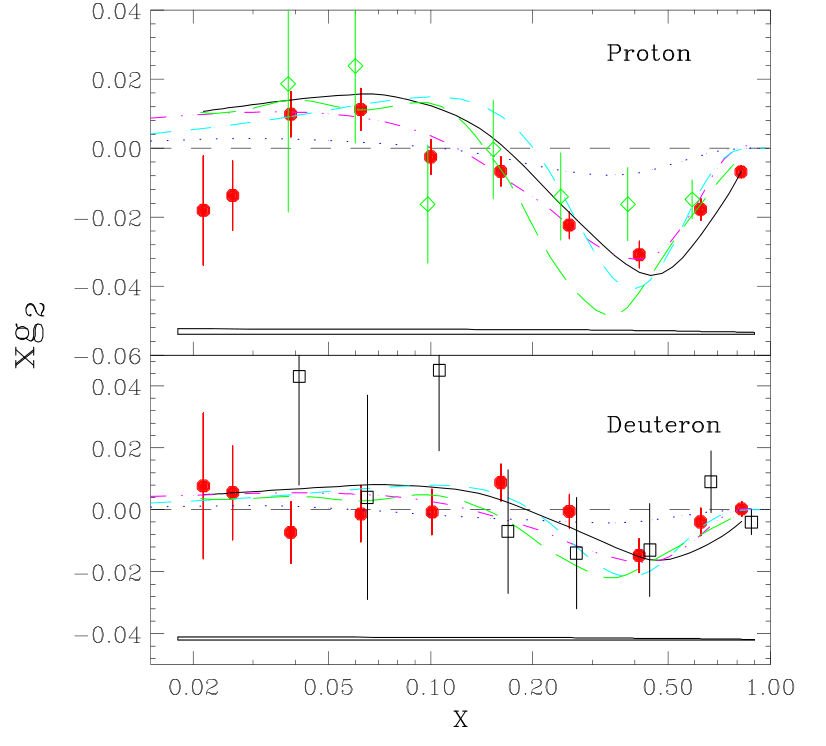
\includegraphics[width=0.75\textwidth]{figs/xg2p_E155x.png}
  \caption[$xg_2$ data from SLAC E155x, E143 and E155.]{$xg_2$ data from E155x (solid circle), E143 (open diamond) and E155 (open square). The $\gtww$ calculation result at the average $Q^2$ of E155x is also shown as the solid line as well as some model estimations from Stratmann \cite{Stratmann1993} (dash-dot), Song \cite{Song1996}(dot), Weigel and Gamberg \cite{Weigel2001} (short dash) and Wakamatsu \cite{Wakamatsu2000} (long dash). Plot reproduced from \cite{Anthony2003}. \label{C4S1F1}}
\end{figure}

The most precise DIS measurement results of $g_2$ for proton and deuteron targets were represented by SLAC experiment E155x \cite{Anthony2003}. The kinematic range was $0.02\leq x\leq 0.8$ and $0.7\leq Q^2 \leq 20$ GeV${}^2$. The SLAC experiments E143 \cite{Abe1998} and E155 \cite{Anthony2003} also contributed to the $g_2$ measurement of proton. The $g_2$ results from SLAC experiments E143, E155 and E155x are shown in \Cref{C4S1F1}. The solid curve in the figure represents the $\gtww$ calculation results using $g_1$ data. The curve shows that the measurement and the leading twist estimation are consistent. However, the large error bars do not exclude the possible higher-twist effects.

As mentioned above, JLab also measured the $g_2$ structure function in the DIS region. The JLab experiment E97-103 measured $g_2$ for neutrons and reported a two standard deviation difference from the leading twist expectation of $g_2^n$ \cite{Kramer2005}. The $Q^2$ coverage of this experiment is $0.58<Q^2<1.36$ GeV${}^2$ at $x\approx0.2$. \Cref{C4S1F2} shows the $xg_2^n$ results from JLab experiments E97-103, E99-117 \cite{Zheng2004} and SLAC experiment E155. The figure clearly represents the deviation between the experimental results and the leading twist estimation.

\begin{figure}[tb!]
  \centering
  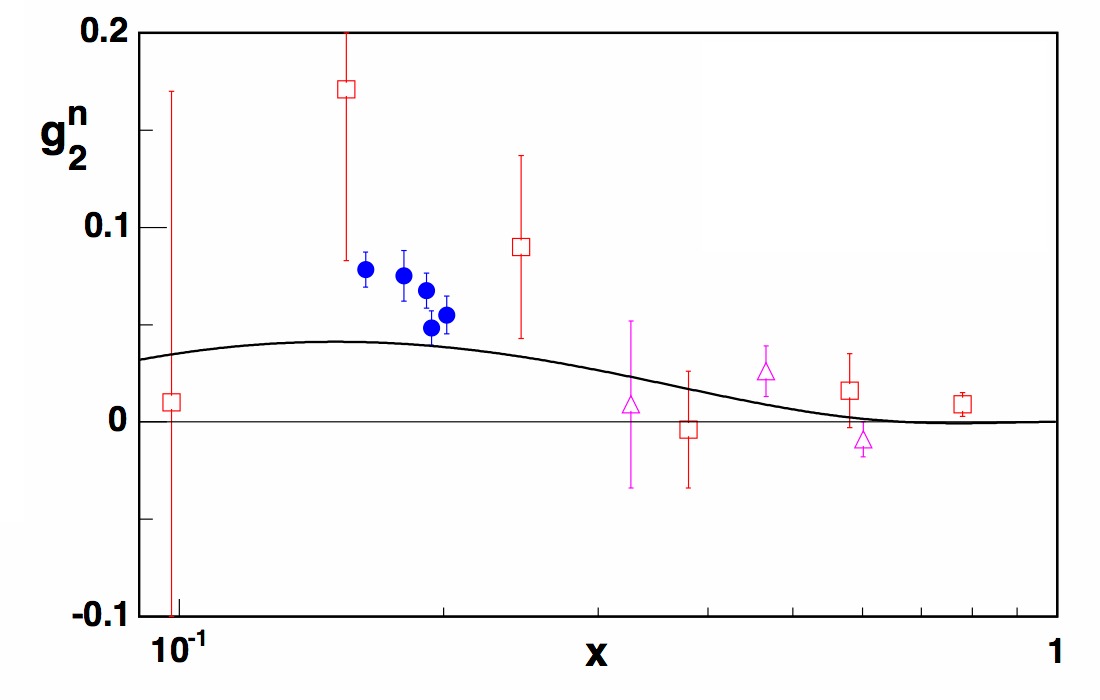
\includegraphics[width=0.6\textwidth]{figs/xg2n_E97103.png}
  \caption[$xg_2^n$ data from E97-103.]{$xg_2^n$ data from E97-103 (solid circle), E99-117 (open triangle) and E155 (open square). The solid curve shows $\gtww$ calculation at $Q^2=1.0$ GeV${}^2$. Plot reproduced from \cite{Kramer2005}. \label{C4S1F2}}
\end{figure}

From the discussion in \Cref{C3S1SS3}, we know that the quark-gluon interaction has a stronger effect in the resonance region. The first experiment to measure $g_2$ in the resonance region was the SLAC experiment E143, at $Q^2=0.5$ GeV${}^2$ and 1.2 GeV${}^2$ \cite{Abe1998}. However the error bar is large for this measurement. JLab E94-010 collected a large amount of data to extract the neutron $g_2$ structure function at low $Q^2$ \cite{Amarian2004a}. The structure function $g_2$ was extracted from the longitudinal and transverse cross-section differences of a polarized ${}^3$He target. The results of ${}^3$He $g_2$ are shown in \Cref{C4S1F3}, which shows a significant deviation from the $\gtww$ estimation.

\begin{figure}[b!]
  \centering
  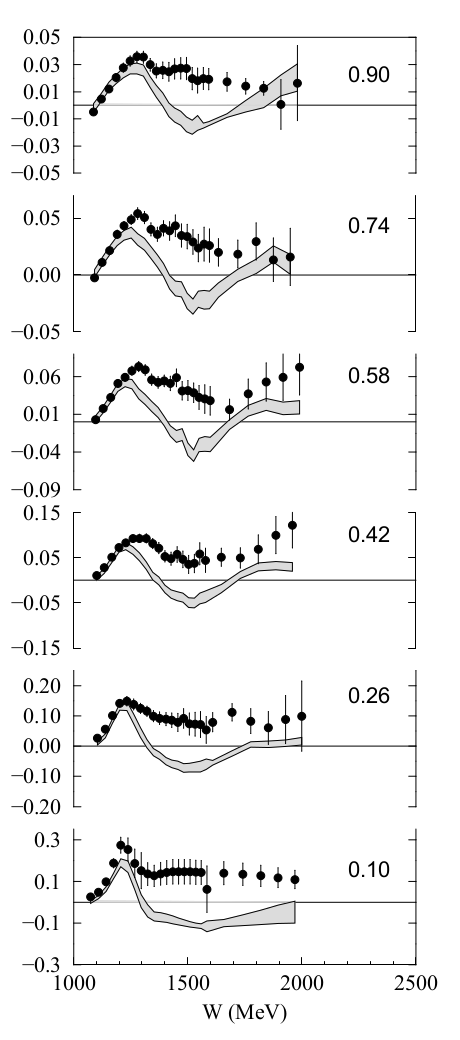
\includegraphics[width=0.55\textwidth]{figs/g2_E94010.png}
  \caption[${}^3$He $g_2$ data from E94-010.]{${}^3$He $g_2$ data from E94-010. The constant $Q^2$ values are indicated in GeV${}^2$ in each panel. The grey bands represent the $\gtww$ expectations at each corresponding $Q^2$ value. Plot reproduced from \cite{Amarian2004a}. \label{C4S1F3}}
\end{figure}

The Resonance Spin Structure (RSS) collaboration in JLab Hall B measured the proton $g_2$ structure function at $Q^2=1.3$ GeV${}^2$ \cite{Wesselmann2007}. Currently this is the lowest $Q^2$ measurement of $g_2^p$. The result is shown in \Cref{C4S1F4}. The leading twist behavior is clearly insufficient to describe the data.

\begin{figure}[tb!]
  \centering
  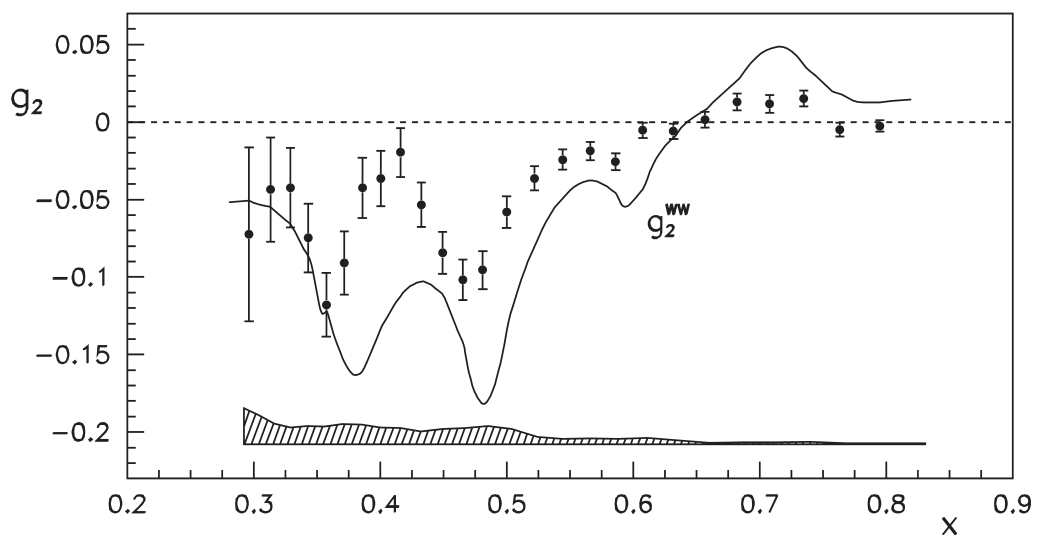
\includegraphics[width=0.75\textwidth]{figs/g2_RSS.png}
  \caption[Proton $g_2$ data from RSS experiment.]{Proton $g_2$ data from RSS experiment compared with the $\gtww$ expectations at $Q^2=1.3$ GeV${}^2$. Plot reproduced from \cite{Wesselmann2007}. \label{C4S1F4}}
\end{figure}

\section[Generalized Longitudinal-Transverse Polarizability]{Generalized Longitudinal-Transverse \\ Polarizability}
\label{C4S2}

\subsection{Sum Rules and Spin Polarizabilities}
\label{C4S2SS1}

In \Cref{C2S4SS2}, we discussed the formulation of real Compton scattering as well as the moments and sum rules which could be extracted from the dispersion relations of the forward real Compton scattering amplitude. Most of that discussions could be generalized for double virtual Compton scattering. In this case, the virtual photon has a third polarization component in addition to the $\epsilon_\pm$ defined in \cref{C2S4E13} due to the longitudinal degree of freedom. The longitudinal polarization vector could be defined as:
\begin{equation} \label{C4S2E1}
\epsilon_0 = \frac{1}{Q}(|\vec{q}|,0,0,q_0),
\end{equation}
where $q$ is the four-momentum of the virtual photon and we have chosen the $z$-axis in the direction of the photon propagation, i.e.,
\begin{equation} \label{C4S2E2}
q = (q_0,0,0,|\vec{q}|).
\end{equation}
All three polarization vectors and the momentum are orthogonal in the Lorentz metrics.

The forward real Compton scattering amplitude \cref{C2S4E17} could be generalized for the VVCS as \cite{Drechsel2003}:
\begin{equation} \label{C4S2E3}
\begin{split}
T(\nu,Q^2,\theta=0) = & \quad \vec{\epsilon}\,'^\star\cdot\vec{\epsilon}f_T(\nu,Q^2)+f_L(\nu,Q^2) \\
& +i\vec{\sigma}\cdot(\vec{\epsilon}\,'^\star\times\vec{\epsilon}\,)g_{TT}(\nu,Q^2)+i\vec{\sigma}\cdot[(\vec{\epsilon}\,'^\star-\vec{\epsilon}\,)\times\hat{q}]g_{LT}(\nu,Q^2).
\end{split}
\end{equation}
Notice the $f(\nu)$ and $g(\nu)$ has been generalized to $f_T(\nu,Q^2)$ and $g_{TT}(\nu,Q^2)$.

Similar to what we did in \Cref{C2S4SS2}, we can apply the optical theorem to \cref{C4S2E3} and get the relations between the four amplitudes and the four partial cross-sections of the inclusive scattering in \cref{C2S4E4}, which gives:
\begin{equation} \label{C4S2E4}
\begin{aligned}
& \Im f_T(\nu,Q^2) = \frac{K}{4\pi}\sigma_T(\nu,Q^2), & \qquad & \Im f_L(\nu,Q^2) = \frac{K}{4\pi}\sigma_L(\nu,Q^2), \\
& \Im g_{TT}(\nu,Q^2) = \frac{K}{4\pi}\stt(\nu,Q^2), & \qquad & \Im g_{LT}(\nu,Q^2) = \frac{K}{4\pi}\slt(\nu,Q^2),
\end{aligned}
\end{equation}
where $K$ is the virtual photon flux defined in \cref{C2S4E2} or \cref{C2S4E3}.

Considering the spin-dependent amplitude $g_{TT}$ and assuming it converges appropriately at high energy, there is an unsubtracted dispersion relation \cite{Drechsel2003}:
\begin{equation} \label{C4S2E5}
\Re[g_{TT}(\nu,Q^2)-g_{TT}^{\mathrm{pole}}(\nu,Q^2)] = \frac{\nu}{2\pi^2}\pv{\int_{\nu_0}^\infty\dd{\nu'}\frac{K(\nu',Q^2)\stt(\nu',Q^2)}{\nu'^2-\nu^2}},
\end{equation}
where $g_{TT}^{\mathrm{pole}}$ is the elastic contribution. The lower limit of the integration $\nu_0$ is the pion-production threshold. As what we did for real Compton scattering, we could also perform a low energy expansion for the non-pole contribution of $g_{TT}$ similar to \cref{C2S4E20}:
\begin{equation} \label{C4S2E6}
\Re[g_{TT}(\nu,Q^2)-g_{TT}^{\mathrm{pole}}(\nu,Q^2)] = \frac{2\alpha}{M^2}I_A(Q^2)\nu+\gamma_0(Q^2)\nu^3+\order{\nu^5}.
\end{equation}

Comparing \cref{C4S2E6} and the Taylor expansion of \cref{C4S2E5}, the $\order{\nu}$ term yields a generalized GDH sum rule \cite{Drechsel2001}:
\begin{equation} \label{C4S2E7}
\begin{split}
I_A(Q^2) & = \frac{M^2}{4\pi^2\alpha}\int_{\nu_0}^\infty\dd{\nu}\frac{K(\nu,Q^2)}{\nu}\frac{\stt(\nu,Q^2)}{\nu}, \\
& = \frac{2M^2}{Q^2}\int_0^{x_0}\dd{x}\left\{g_1(x,Q^2)-\frac{4M^2}{Q^2}x^2g_2(x,Q^2)\right\}.
\end{split}
\end{equation}
The $\order{\nu^3}$ term leads to a generalized form of the forward spin polarizability $\gamma_0$:
\begin{equation} \label{C4S2E8}
\begin{split}
\gamma_0(Q^2) & = \frac{1}{2\pi^2}\int_{\nu_0}^\infty\dd{\nu}\frac{K(\nu,Q^2)}{\nu}\frac{\stt(\nu,Q^2)}{\nu^3}, \\
& = \frac{16\alpha M^2}{Q^6}\int_0^{x_0}\dd{x}x^2\left\{g_1(x,Q^2)-\frac{4M^2}{Q^2}x^2g_2(x,Q^2)\right\}.
\end{split}
\end{equation}
The term proportional to $g_2$ can be dropped when $Q^2$ is large.

For amplitude $g_{LT}$, we have an unsubtracted dispersion relation in the form of \cite{Drechsel2003}:
\begin{equation} \label{C4S2E9}
\Re[g_{LT}(\nu,Q^2)-g_{LT}^{\mathrm{pole}}(\nu,Q^2)] = \frac{1}{2\pi^2}\pv{\int_{\nu_0}^\infty\dd{\nu'}\frac{\nu'K(\nu',Q^2)\slt(\nu',Q^2)}{\nu'^2-\nu^2}}.
\end{equation}
The low energy expansion of the non-pole contribution of $g_{LT}$ gives:
\begin{equation} \label{C4S2E10}
\Re[g_{LT}(\nu,Q^2)-g_{LT}^{\mathrm{pole}}(\nu,Q^2)] = \frac{2\alpha}{M^2}QI_3(Q^2)\nu+Q\dlt(Q^2)\nu^2+\order{\nu^4},
\end{equation}
where the leading term is a sum rule for $I_3(Q^2)$:
\begin{equation} \label{C4S2E11}
\begin{split}
I_3(Q^2) & = \frac{M^2}{4\pi^2\alpha}\int_{\nu_0}^\infty\dd{\nu}\frac{K(\nu,Q^2)}{\nu}\frac{\slt(\nu,Q^2)}{Q}, \\
& = \frac{2M^2}{Q^2}\int_0^{x_0}\dd{x}\left\{g_1(x,Q^2)+g_2(x,Q^2)\right\},
\end{split}
\end{equation}
and the $\order{\nu^2}$ gives the generalized longitudinal-transverse polarizability:
\begin{equation} \label{C4S2E12}
\begin{split}
\dlt(Q^2) & = \frac{1}{2\pi^2}\int_{\nu_0}^\infty\dd{\nu}\frac{K(\nu,Q^2)}{\nu}\frac{\slt(\nu,Q^2)}{Q\nu^2}, \\
& = \frac{16\alpha M^2}{Q^6}\int_0^{x_0}\dd{x}x^2\left\{g_1(x,Q^2)+g_2(x,Q^2)\right\}.
\end{split}
\end{equation}

The forward VVCS amplitude $T(\nu,Q^2,\theta=0)$ can also be written in the form of an one-to-one correspondence with the structure functions \cite{Drechsel2003}:
\begin{equation} \label{C4S2E13}
\begin{split}
T(\nu,Q^2,\theta=0) = \epsilon_\mu'^{\star}\epsilon_\nu & \left\{\left(\frac{q^\mu q^\nu}{q^2}-g^{\mu\nu}\right)T_1(\nu,Q^2)\right. \\
& +\frac{1}{P\cdot q}(P^\mu-\frac{P\cdot q}{q^2}q^\mu)(P^\nu-\frac{P\cdot q}{q^2}q^\nu)T_2(\nu,Q^2) \\
& +i\varepsilon^{\mu\nu\alpha\beta}\frac{1}{M}q_\alpha S_\beta S_1(\nu,Q^2) \\
& \left.+i\varepsilon^{\mu\nu\alpha\beta}\frac{1}{M^3}q_\alpha(P\cdot qS_\beta-S\cdot qP_\beta)S_2(\nu,Q^2)\right\},
\end{split}
\end{equation}
where $P^\mu$ and $S^\mu$ are the four momentum and the spin vector of the nucleon and $T_1$, $T_2$, $S_1$, $S_2$ are four VVCS amplitudes which is covariant under Lorentz transform.

Since we only discussed te spin-flip amplitudes $g_{TT}$ and $g_{LT}$ in this section, we will focus on $S_1$ and $S_2$, which can be expressed as a linear combination of $g_{TT}$ and $g_{LT}$:
\begin{equation} \label{C4S2E14}
\begin{split}
S_1(\nu,Q^2) & = \frac{\nu M}{\nu^2+Q^2}\left(g_{TT}(\nu,Q^2)+\frac{Q}{\nu}g_{LT}(\nu,Q^2)\right), \\
S_2(\nu,Q^2) & = -\frac{M^2}{\nu^2+Q^2}\left(g_{TT}(\nu,Q^2)-\frac{\nu}{Q}g_{LT}(\nu,Q^2)\right).
\end{split}
\end{equation}
We can construct unsubtracted dispersion relations for $S_1$ and $S_2$ with a similar procedure as $g_{LT}$ and $g_{TT}$.

For amplitude $S_1$, the low energy expansion has the form:
\begin{multline} \label{C4S2E15}
\Re[S_1(\nu,Q^2)-S_1^{\mathrm{pole}}(\nu,Q^2)] = \\
\frac{2\alpha}{M^2}I_1(Q^2)+\left[\frac{2\alpha}{MQ^2}(I_A(Q^2)-I_1(Q^2))+M\dlt(Q^2)\right]\nu^2+\order{\nu^4},
\end{multline}
where the leading term leads to a sum rule:
\begin{equation} \label{C4S2E16}
\begin{split}
I_1(Q^2) & \equiv \frac{2M^2}{Q^2}\int_0^{x_0}\dd{x}g_1(x,Q^2) \\
& = \frac{M^2}{4\pi^2\alpha}\int_{\nu_0}^\infty\dd{\nu}\frac{K(\nu,Q^2)}{\nu^2+Q^2}\left\{\stt(\nu,Q^2)+\frac{Q}{\nu}\slt(\nu,Q^2)\right\},
\end{split}
\end{equation}
which reduces to the GDH sum rule at $Q^2=0$ (real photon limit). $I_1(Q^2)$ has a limit at large $Q^2$:
\begin{equation} \label{C4S2E17}
I_1(Q^2)\rightarrow(2M^2/Q^2)\Gamma_1(Q^2), \qquad Q^2\rightarrow\infty,
\end{equation}
where
\begin{equation} \label{C4S2E18}
\Gamma_1(Q^2) \equiv \int_0^1\dd{x}g_1(x,Q^2).
\end{equation}
Here the $\Gamma_1$ is the first moment of structure function $g_1$. The Bjorken sum rule \cite{Bjorken1966,Bjorken1970} gives a prediction of the isovector combination $\Gamma_1^p-\Gamma_1^n$ with the QCD radiative corrections \cite{Larin1991}:
\begin{multline} \label{C4S2E19}
\Gamma_1^p-\Gamma_1^n = \frac{1}{6}g_A \\
\times\left\{1-\left(\frac{\alpha_S(Q^2)}{\pi}\right)-3.5833\left(\frac{\alpha_S(Q^2)}{\pi}\right)^2-20.2153\left(\frac{\alpha_S(Q^2)}{\pi}\right)^3+\cdots\right\},
\end{multline}
where $g_A$ is the axial-vector coupling constant. At $Q^2=5$ GeV${}^2$, \cref{C4S2E19} gives $\Gamma_1^p-\Gamma_1^n=0.182\pm0.005$ if only the three light quark flavors are considered. The next-to-leading order fit to global $g_1$ data gives $\Gamma_1^p-\Gamma_1^n=0.176\pm0.003\pm0.007$ \cite{Anthony2000}, in agreement with the theoretical calculation.

The unsubtracted dispersion relations of the amplitude $S_2$ lead to the Burkhardt-Cottingham sum rule. Assume the high energy behavior of this amplitude is given by $S_2\rightarrow\nu^{\alpha_2}$ with $\alpha_2<-1$ when $\nu\rightarrow\infty$, there should be a dispersion relation for $\nu S_2$. By subtracting the dispersion relation of $\nu S_2$ from the dispersion relation of $S_2$ multiplied by $\nu$, we could get a ``super-convergence relation'' \cite{Burkhardt1970}:
\begin{equation} \label{C4S2E20}
\int_0^1\dd{x}g_2(x,Q^2) = 0.
\end{equation}
This indicates that the elastic and the inelastic contributions to the first moment of $g_2$ should cancel for any value of $Q^2$. The elastic and inelastic contributions to the integral can be separated, thus the BC sum rule can be expressed as:
\begin{equation} \label{C4S2E21}
I_2(Q^2) \equiv \frac{2M^2}{Q^2}\int_0^{x_0}\dd{x}g_2(x,Q^2) = \frac{1}{4}F_P(Q^2)(F_D(Q^2)+F_P(Q^2)),
\end{equation}
where $F_P$ is the Pauli form factor and $F_D$ is the Dirac form factor. The integral $I_2$ can also be written in terms of the photon-absorption cross-sections and the Sachs form factor $G_E$ and $G_M$:
\begin{equation} \label{C4S2E22}
\begin{split}
I_2(Q^2) & = \frac{M^2}{4\pi^2\alpha}\int_{\nu_0}^\infty\frac{K(\nu,Q^2)}{\nu^2+Q^2}\left\{-\stt(\nu,Q^2)+\frac{\nu}{Q}\slt(\nu,Q^2)\right\} \\
& = \frac{1}{4}\frac{G_M(Q^2)(G_M(Q^2)-G_E(Q^2))}{1+\tau},
\end{split}
\end{equation}
with $\tau=Q^2/4M^2$.

\subsection{Existing World Data for Spin Polarizabilities}
\label{C4S2SS2}

From the discussion in \Cref{C2S4SS2}, we know that the nucleon polarizabilities are fundamental observables that characterize nucleon structure. The electric and magnetic polarizabilities $\alpha$ and $\beta$ describe the response of a nucleon to an external electromagnetic field. Real photon Compton scattering experiments were performed to measure these two quantities since they are related to the spin non-flip forward Compton scattering amplitude \cite{Olmos2001,Tonnison1998}. The forward spin polarizability $\gamma_0$ is associated with the spin flip amplitude. It has been measured at MAMI (Mainz) with a circularly polarized photon beam on a longitudinally polarized proton target \cite{Ahrens2001}.

In the previous section, we have discussed that these polarizabilities could be generalized in VVCS. The generalized polarizabilities defined in \cref{C4S2E8,C4S2E12} have an extra $1/\nu^2$ weighting in the integrand compared to the corresponding leading moments. Thus, the contribution of the large-$\nu$ region to these integrals are suppressed by this weight. With this suppression effect, the generalized spin polarizabilities become a perfect tool to probe the nucleon structure in the chiral perturbation region. The generalized polarizabilities have been evaluated with next-to-leading order (NLO) $\chi$PT calculations at low $Q^2$ \cite{Bernard2003,Kao2003}. As mentioned in \Cref{C3S1SS3}, the nucleon resonances, especially the $\Delta$ resonance, play an important role in the $\chi$PT calculations. Ref. \cite{Bernard2003} and \cite{Kao2003} have pointed out that the generalized longitudinal polarizability $\dlt$ is insensitive to the $\Delta$ resonance compare with the generalized forward spin polarizability $\gamma_0$. The effects from the $\Delta$ resonance contribution are expected to be important in $\gamma_0$ but are supposed to largely cancel in $\dlt$.

\begin{figure}[tb!]
  \centering
  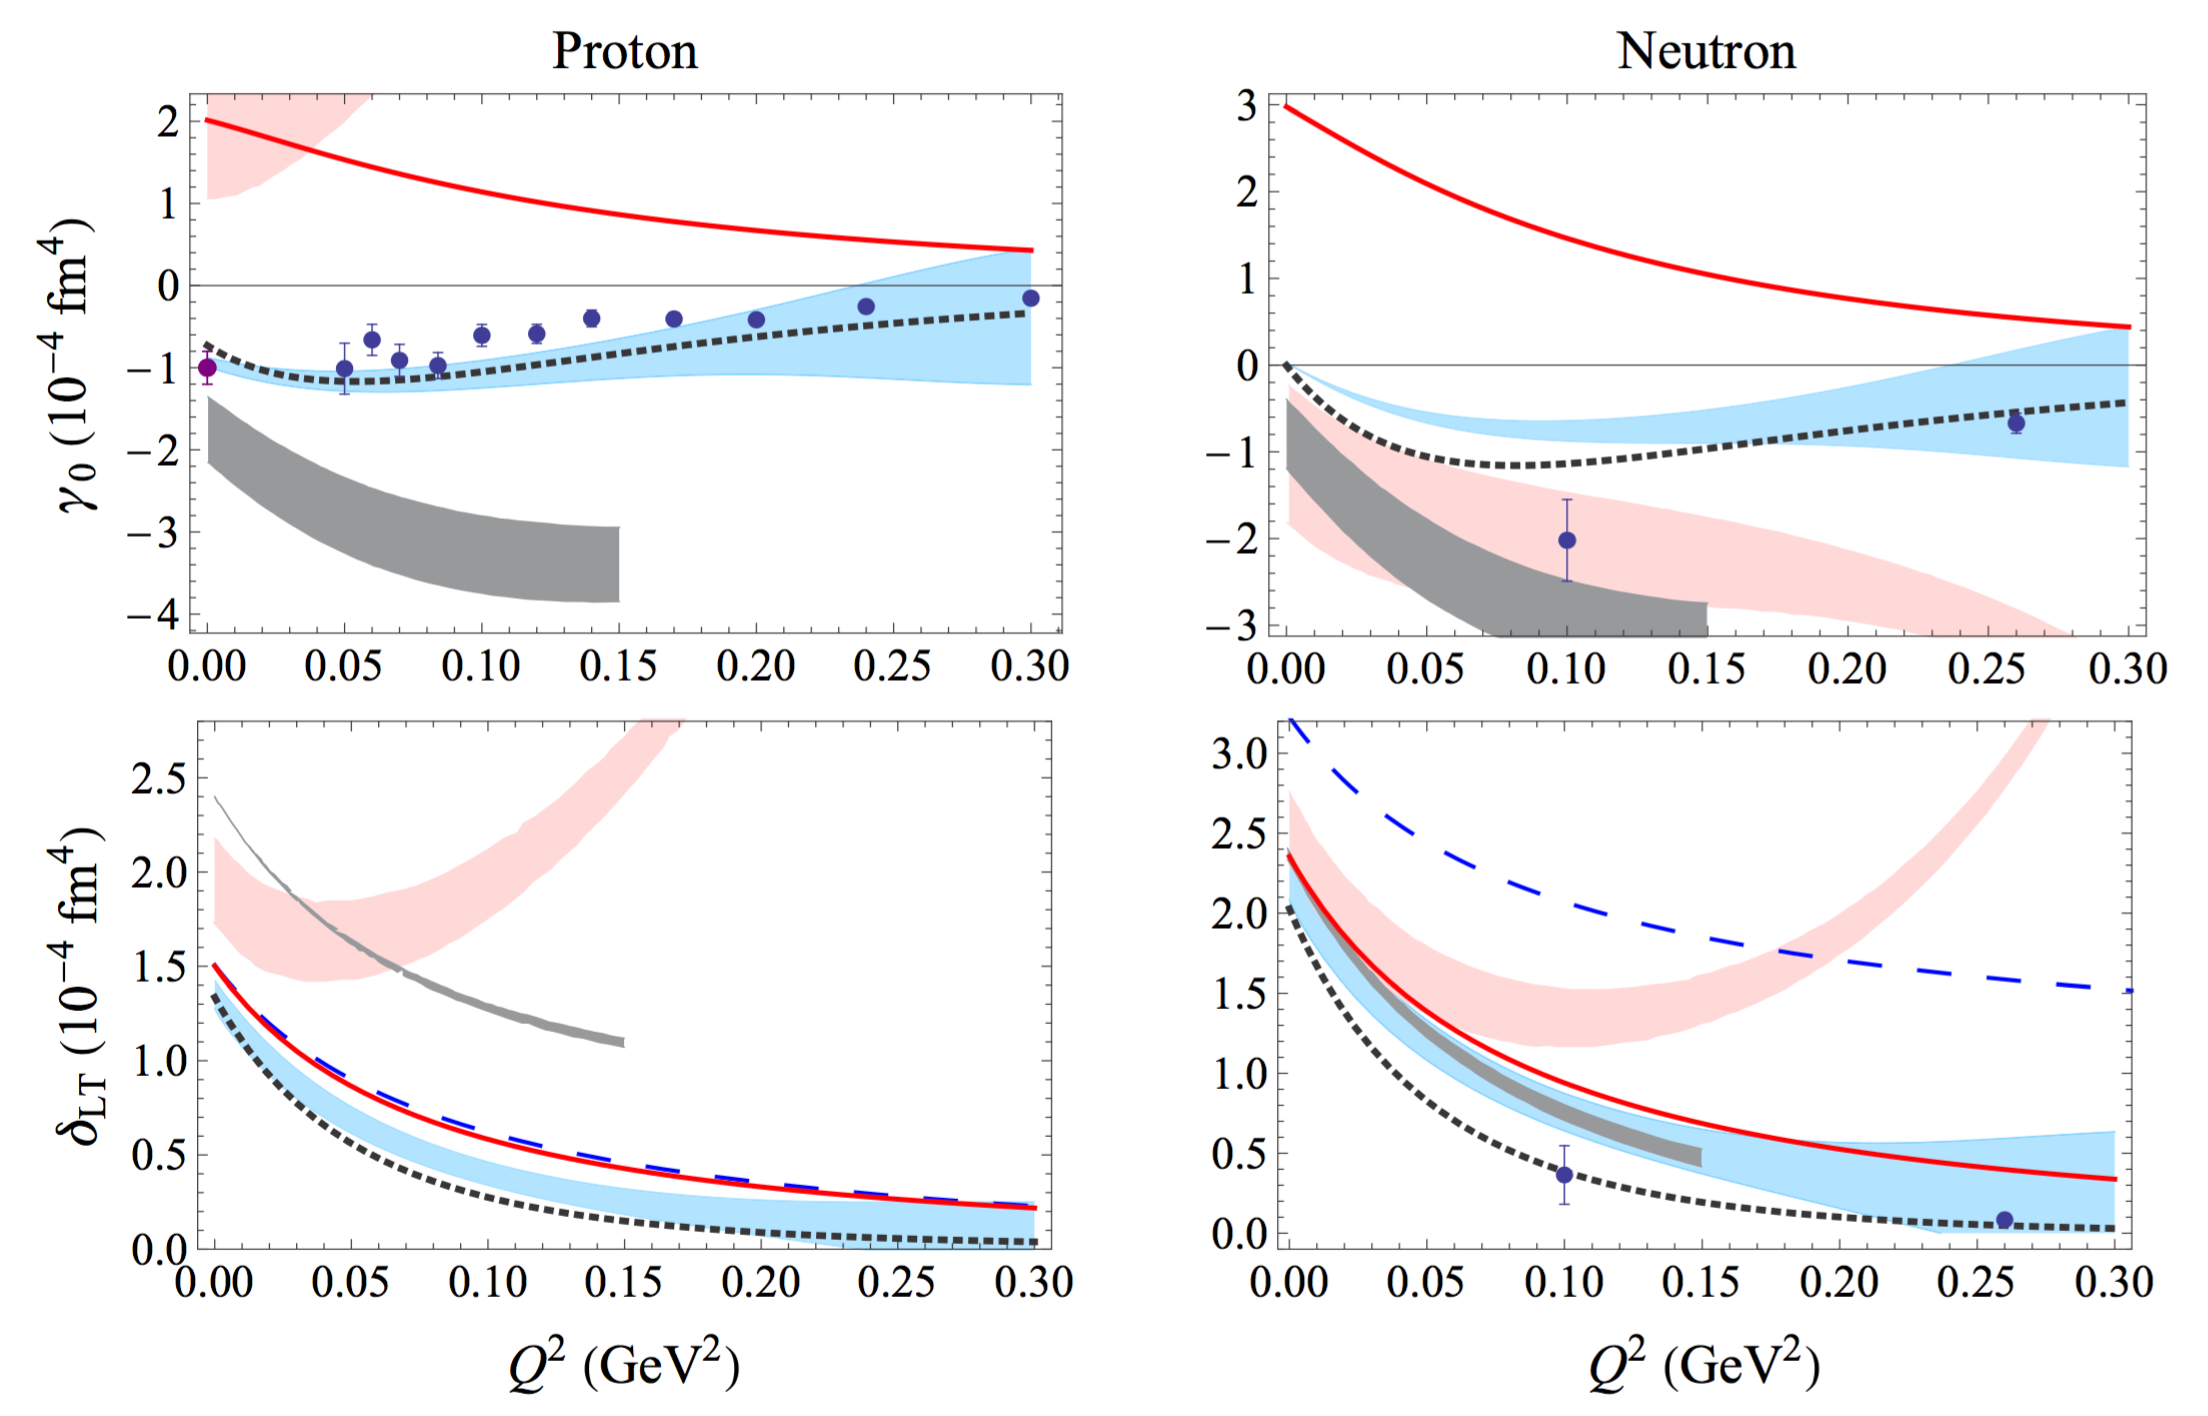
\includegraphics[width=\textwidth]{figs/g0_dlt_xpt.png}
  \caption[Generalized spin polarizability $\gamma_0$ and $\dlt$ of proton and neutron.]{Generalized spin polarizability $\gamma_0$ and $\dlt$ of proton and neutron. The neutron data are from E94-010 experiment \cite{Amarian2004b}. The proton data at $Q^2=0$ (purple dot) are from ELSA \cite{Dutz2003}, and at finite $Q^2$ (blue dots) from EG1 experiment at JLab \cite{Prok2009}. The blue dashed line is the HB$\chi$PT calculation \cite{Kao2003}, off the scale in the upper panels. The red bands shows the IR version of RB$\chi$PT calculation \cite{Bernard2003}. The grey bands are the first RB$\chi$PT calculation from Ref. \cite{Bernard2013}. The red solid lines and blue bands shows the most recent LO and NLO RB$\chi$PT calculations respectively \cite{Lensky2014}. Black dotted lines represents the empirical evaluation using the Mainz online partial-wave analysis of meson electroproduction (MAID). Plot reproduced from \cite{Lensky2014}. \label{C4S2F1}}
\end{figure}

The experimental results compared with the $\chi$PT calculations are shown in \Cref{C4S2F1}. The first results of neutron $\gamma_0(Q^2)$ and $\dlt(Q^2)$ were obtained from JLab Hall A experiment E94-010 \cite{Amarian2004b} (blue dots in the neutron panels). The data are compared with a HB$\chi$PT calculation \cite{Kao2003} (blue dashed line) and an infrared-regularized (IR) version of RB$\chi$PT calculation \cite{Bernard2003} (red bands) which is relativisitic but has an unphysical analytic structure. At the lowest $Q^2$ point, the IR version of RB$\chi$PT calculation of $\gamma_0$ including the resonance contributions agrees with the experimental result from E94-010 for neutron. But there are discrepancies between the HB$\chi$PT calculation of $\gamma_0$ and the experimental result even at the lowest $Q^2$ point. For $\dlt$, both the HB$\chi$PT calculation and the IR version of RB$\chi$PT calculation indicates a significant disagreement with the data, which is known as the ``$\dlt$ puzzle''. Since the $\dlt$ is insensitive to the $\Delta$ resonance contribution, it is believed that $\dlt$ is a more suitable testing base for the $\chi$PT compare with $\gamma_0$. A first RB$\chi$PT calculation (with no unphysical analytical structure) from Ref. \cite{Bernard2013} shows that it agrees much better than the HB$\chi$PT and the IR version of the RB$\chi$PT for $\gamma_0$ (grey bands). The most recent calculation from Ref. \cite{Lensky2014} using LO and NLO RB$\chi$PT shows that the $\dlt$ data agrees with their NLO calculation (blue bands). The neutron $\gamma_0$ and $\dlt$ data in \Cref{C4S2F1} is obtained from the JLab experiment E94-010. The proton $\dlt$ data is required to complete the comparison. This is one of the major physics motivation of the JLab experiment E08-027.

\section{Burkhardt-Cottingham Sum Rule}
\label{C4S3}

In \Cref{C4S2SS1}, we have discussed the dispersion relations for the covariant spin-dependent VVCS amplitudes $S_2$. The dispersion relations for $S_2$ and $\nu S_2$ lead to a sum rule for $g_2$ which is valid for all $Q^2$ \cite{Burkhardt1970}:
\begin{equation} \label{C4S3E1}
\Gamma_2(Q^2) = \int_0^1\dd{x}g_2(x,Q^2) = 0.
\end{equation}
The existence of the dispersion relation of $\nu S_2$ requires $S_2\rightarrow\nu^{\alpha_2}$ with $\alpha_2<-1$ when $\nu\rightarrow\infty$. Thus, the convergence condition of the integral leads to $g_2(x,Q^2)\rightarrow x^{\tilde{\alpha}_2}$ with $\tilde{\alpha}_2>-1$ when $x\rightarrow0$, which means that $g_2$ must exhibit Regge behavior at low $x$ and does not exhibit a delta function singularity at $x=0$ \cite{Jaffe1991}.

The first measurement of the moment $\Gamma_2$ is the SLAC experiment E155, which included the result of proton, deuteron and neutron. JLab Hall A has collected a large amount of data to extract the BC integral of neutron over a wide kinematic range in several experiments: E94-010 \cite{Amarian2004a}, E97-110 and E01-012. Since it is impossible to cover the full integral range, the full ($0<x<1$) integral is evaluated using the elastics form factors for the elastic contribution, and assuming $g_2=\gtww$ in the very low-$x$ region. The full integral exhibits a significant cancellation of the inelastic (resonance and DIS) and elastic contributions. The neutron data agrees with the BC sum rule prediction within uncertainty.

\begin{figure}[tb!]
  \centering
  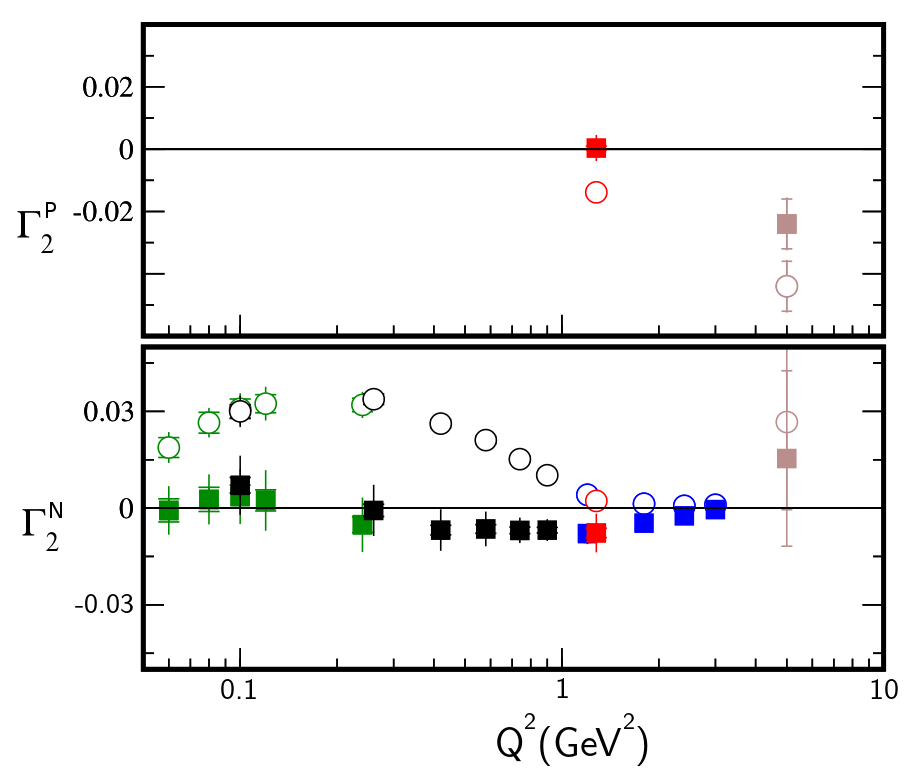
\includegraphics[width=0.75\textwidth]{figs/BC_all.png}
  \caption[The verification of the BC sum rule.]{The verification of the BC sum rule from JLab Hall C experiment RSS (red) and Hall A experiments E94-010 \cite{Amarian2004a} (black), E97-110 (green) and E01-012 (blue), together with SLAC experiment E155x \cite{Anthony2003} (brown). The open circles are the measured values and the solid squares are the total moments including the elastic and estimated contributions from high energy region. The data from experiments RSS and E97-110 are still preliminary. Plot reproduced from \cite{Chen2010}. \label{C4S3F1}}
\end{figure}

On the other hand, the proton BC integral deviated from zero by three standard deviations in SLAC experiment E155x \cite{Abe1998}. E155x covered the $x$ range from 0.02 to 0.8 and its $Q^2$ coverage $0.8-8.2$ GeV${}^2$ was averaged to 5 GeV${}^2$. JLab experiment RSS also measured the BC integral for proton which covered $W<1.910$ MeV at $Q^2\approx1.3$ GeV${}^2$. The preliminary result agrees with the BC sum rule prediction within the experimental error. The experimental results for verification of the BC sum rule are summarized in \Cref{C4S3F1}.

\section{Proton Hyperfine Structure}
\label{C4S4}

The hydrogen hyperfine splitting has been measured to a relative accuracy of $10^{-13}$ according to the discussion in Ref. \cite{Nazaryan2006}:
\begin{equation} \label{C4S4E1}
\Delta E = 1420.405 751 766 7(9) \text{MHz}.
\end{equation}
This value could be calculate in QED. $\Delta E$ can be expressed in terms of the so-called Fermi energy $E_F$ which is the leading order contribution to the ground state hyperfine splitting as $\Delta E = (1+\delta)E_F$, where the correction $\delta$ is given by:
\begin{equation} \label{C4S4E2}
\delta = 1+(\delta_{\mathrm{QED}}+\delta_R+\delta_{\mathrm{small}})+\Delta_S.
\end{equation}
Here the $\delta_{\mathrm{QED}}$ represents the QED radiative correction which has been calculated to very high accuracy. The $\delta_R$ accounts the recoil effects and the $\delta_{\mathrm{small}}$ term contains all other small corrections such as the weak interaction correction.

The $\Delta_S$ term in \cref{C4S4E2} represents the proton structure correction which has the largest uncertainty. $\Delta_S$ is conventionally split into two terms:
\begin{equation} \label{C4S4E3}
\Delta_S = \Delta_Z+\Delta_{\mathrm{pol}},
\end{equation}
where $\Delta_Z$ can be determined from elastic scattering \cite{GEP} and $\Delta_{\mathrm{pol}}$ contains the contributions from excited proton \cite{Iddings1965,Faustov2002}:
\begin{equation} \label{C4S4E4}
\Delta_{\text{pol}} = \frac{\alpha m_e}{\pi g_pm_p}(\Delta_1+\Delta_2),
\end{equation}
where $\Delta_1$ involves the Pauli form factor and the $g_1$ structure function, and $\Delta_2$ only depends on the $g_2$ structure function:
\begin{equation} \label{C4S4E5}
\Delta_2 = -24m_p^2\int_0^{\infty}\frac{\dd{Q}^2}{Q^4}B_2(Q^2),
\end{equation}
where
\begin{equation} \label{C4S4E6}
B_2(Q^2) = \int_0^{x_{\mathrm{th}}}\dd{x}\beta_2(\tau)g_2(x,Q^2).
\end{equation}
and
\begin{equation} \label{C4S4E7}
\beta_2(\tau) = 1+2\tau-2\sqrt{\tau(\tau+1)},
\end{equation}
with $\tau=\nu^2/Q^2$ and $x_{\mathrm{th}}$ is the pion production threshold.

$\Delta_1$ could be determined with data but to evaluate $\Delta_2$ physicists still heavily rely on models since proton $g_2$ data are still lacking. The $Q^2$ weighting in \cref{C4S4E5} indicates that $\Delta_2$ is dominated by the contribution at low $Q^2$ \cite{Nazaryan2006}. Thus, precision data of proton $g_2$ at low $Q^2$ is needed to evaluate $\Delta_2$.

%%%%%%%%%%%%%%%%%%%%%%%%%%%%%%%%%%%%%%%%%%%%%%%%%%%%%%%%%%%%%%%%%%%%%%
% -*-latex-*-

% -*-latex-*-

\chapter{The Experiment}
\label{C5}

Experiment E08-027 was conducted in Hall A at Thomas Jefferson National Accelerator Facility (Jefferson Lab or JLab) from March to May, 2012 at Jefferson Lab. The experiment was a precise measurement of the inclusive polarized cross-section for electron scattering from proton. The main goal of this experiment is to extract the proton spin-dependent structure function $g_2$ in the resonance region with $0.02<Q^2<0.20$ GeV${}^2$ \cite{G2P}. The measured $g_2^p$ data allow us to extract the longitudinal-transverse spin polarizability $\dlt$ for proton to perform a benchmark test of $\chi$PT predictions and to test the BC sum rule as we already discussed in \Cref{C4}.

During experiment E08-027, a longitudinally polarized electron beam with four different incident energies between 1.157 and 3.350 GeV were scattered from a transversely polarized proton target to measure the transverse polarized cross-section differences $\Delta\sigma_\perp$. The Hall A High Resolution Spectrometer (HRS) was used to detect the scattered electrons at an angle of \SI{5.77}{\degree}. The $\Delta\sigma_\perp$ data was combined with the longitudinal polarized cross-section differences $\Delta\sigma_\parallel$ from JLab Hall B EG4 experiment in the same kinematic region to extract proton $g_2$ structure function. The $\Delta\sigma_\parallel$ data was also collected in E08-027 with a longitudinally polarized NH${}_3$ target at 2.254 GeV incident beam energy to verify the EG4 data.

\begin{figure}[tb!]
  \centering
  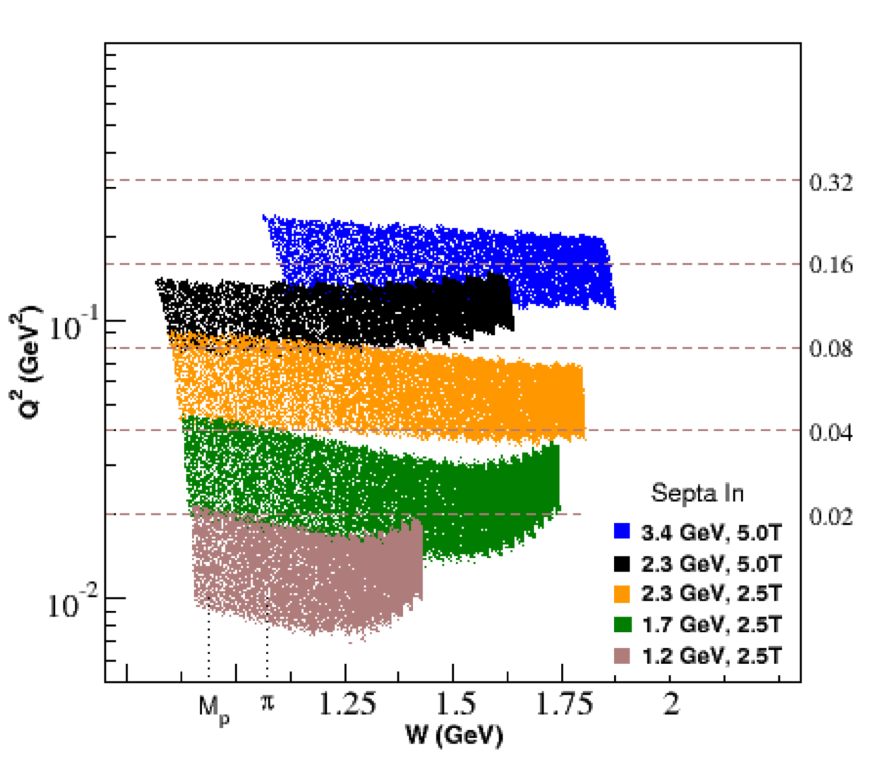
\includegraphics[width=0.75\textwidth]{figs/kinematics-g2p.png}
  \caption[Kinematic coverage of experiment E08-027.]{Kinematic coverage of experiment E08-027. The legend shows the beam energy and target field strength for each setting. Plot reproduced from \cite{G2P}. \label{C5F1}}
\end{figure}

The data were acquired in four different beam energy and two different target field configurations. The kinematic coverage of each setting is shown in \Cref{C5F1}. Only those settings with the transverse target field are included in the figure. Since the minimum angle limit of the HRS is \SI{12.5}{\degree} \cite{Alcorn2004}, a septum magnet was installed in front of the spectrometer pair to bend the $\sim$\SI{5.77}{\degree} scattered electrons into the HRS. Unfortunately, portions of the septum magnet coils were burned twice during the experiment, which led to three different septum configurations. The experiment configurations are summarized in \cref{C6S3T1} while we discuss the spectrometer optics study in \Cref{C6S3SS1}.

The polarized proton was provided by a frozen ammonia target in E08-027. The Dynamic Nuclear Polarization (DNP) process was used to polarize the target. Beam current was limited up to 50 nA during the experiment to reduce the depolarization of the target. However, the standard Hall A beamline electronics were not designed to work with such low beam currents. Thus new beam current monitors (BCMs) and beam position monitors (BPMs) which could work at very low beam currents were used in this experiment. To further reduce the depolarization effect, a pair of slow rasters were installed in Hall A for the first time to spread the beam over the target uniformly. Since the strong transverse target field would bend the incident and the scattered electrons, two chicane dipole magnets were installed in Hall A upstream of the target to compensate the effect of the target field. A local beam dump was also installed downstream of the target to stop the electron beam when it could not reach the standard beam dump of Hall A due to the effect of the target field. \Cref{C5F2} is a schematic diagram indicating major experimental components of E08-027.

\begin{figure}[tb!]
  \centering
  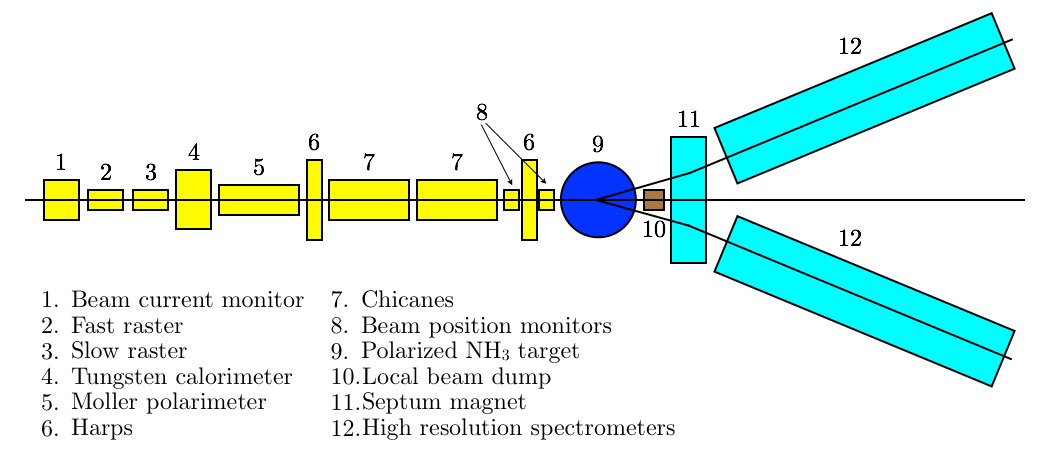
\includegraphics[width=\textwidth]{figs/experiment-setup.png}
  \caption[Schematic diagram of the experiment components.]{Schematic diagram of the experiment components. \label{C5F2}}
\end{figure}

This chapter will discuss the electron beam, the Hall A beamline components, the polarized ammonia target and the HRS system. It is crucial to understand these components in a precise measurement of the polarized cross-sections.

\section{The Electron Accelerator}
\label{C5S1}

\subsection{Continuous Electron Beam Accelerator Facility}
\label{C5S1SS1}

The superconducting radio-frequency Continuous Electron Beam Accelerator Facility (CEBAF) at JLab consists of a polarized electron source, an injector, two linacs, two recirculation arcs and extraction elements to send beam into three experimental halls: A, B and C \footnote{Following the 12 GeV upgrade of Jefferson lab, which was carried out after this experiment, a fourth experimental hall, Hall D was added.} \cite{Sulkosky2007}. \Cref{C5S1F1} is a sketch of the CEBAF accelerator.

\begin{figure}[tb!]
  \centering
  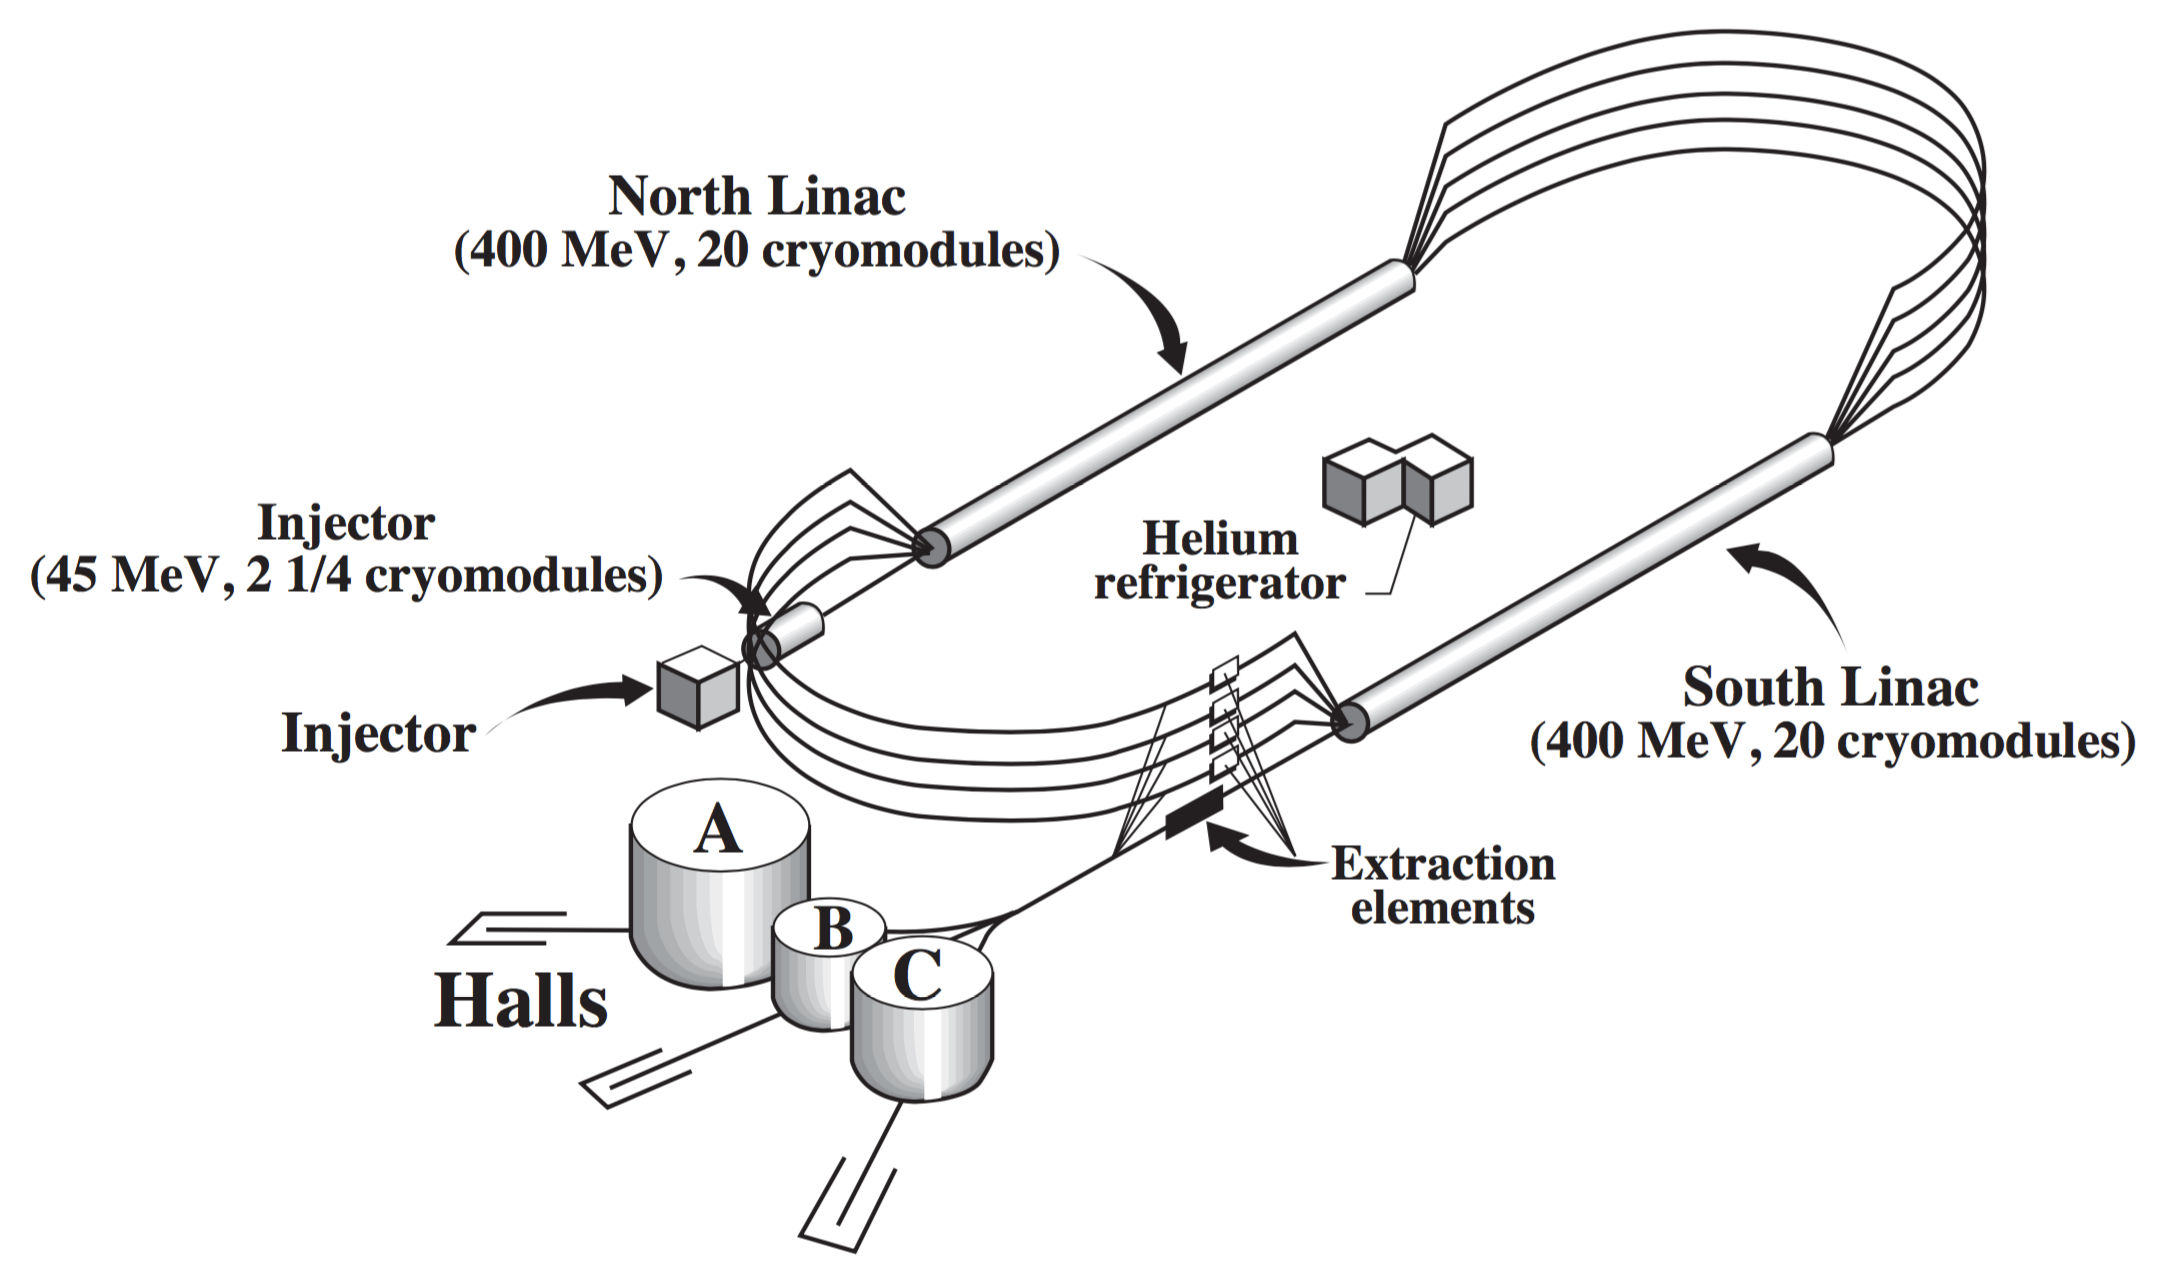
\includegraphics[width=0.7\textwidth]{figs/accelerator.png}
  \caption[Sketch of the CEBAF accelerator.]{Sketch of the CEBAF accelerator. The beam travels once through the North and South linacs with each recirculation, when part of it could be extracted to any of the three Halls. The linac energies shown are for operation at 4 GeV; at 6 GeV each linac operates at 600 MeV. Plot reproduced from \cite{Gross2011}. \label{C5S1F1}}
\end{figure}

Once the electron beam is generated, it is injected into the accelerator after initial acceleration to 45 MeV. A Wien filter is used at the injector to set the polarization angle of the electrons. The precession of the electrons is taken into account to assure that the electrons are longitudinally polarized when they reach the experimental halls. As shown in \Cref{C5S1F1}, the main acceleration part is composed of two anti-parallel linacs linked by nine recirculation arcs for up to five passes. Each linac can be used to accelerate electrons for all passes since the electrons are ultra-relativistic and travel at almost the same speed. At the end of the second linac, the beam can either enter the recirculation arc to be accelerated one more pass or be extracted into the experimental halls.

CEBAF can provide electron beams at different but correlated energies to three experimental halls simultaneously. The accelerator was originally designed to be operated with a maximum beam energy around 4 GeV. However the maximum achieved beam energy reached nearly 6 GeV with the state-of-arts superconducting radio-frequency technologies. The maximum total beam current available among the three halls is 200 $\mu$A. The current can be split arbitrarily between three inter-leaved 499 MHz bunches. Each of the bunches can then be peeled off to any one of the halls \cite{Sulkosky2007}. CEBAF has provided electron beams at 1-150 $\mu$A for experimental Hall A and C and 1-100 nA for experimental Hall B since 2000.

\subsection{Beam Helicity}
\label{C5S1SS2}

At Jefferson Lab, the polarized electron beam is produced by illuminating a GaAs photocathode with circularly polarized photons \cite{Gross2011}. The beam helicity need to be reversed to measure helicity-dependent observables like the cross-section differences in E08-027. The spin of the photo-emitted electron is correlated to the circular polarization state of the photon. It can be either aligned parallel (1 or +) or anti-parallel (0 or -) to the electron momentum direction, which are the two helicity states of the electron. Thus the beam helicity can be reversed by changing the polarization state of the light.

\begin{figure}[b!]
  \centering
  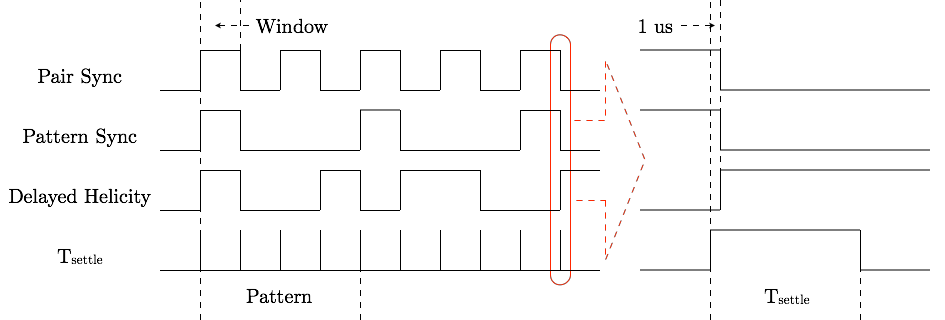
\includegraphics[width=\textwidth]{figs/helicity-signal.png}
  \caption[Helicity signals received by experiment DAQ.]{Helicity signals received by experiment DAQ. The right side shows the time sequence of these signals, notice that the $\tsettles$ signal is 1 $\mu$s prior to the other three to avoid misalignment. \label{C5S1F2}}
\end{figure}

A programmable logic generator known as the Helicity Control Board is installed at the injector to control the helicity of the electron beam \cite{Flood2010}. It generates a logic signal known as the Helicity Flip signal to control the polarity of the high voltage of the Pockels Cell on the Laser Table in the injector. The Pockels Cell is a crystal that acts as a quarter-wave retardation plate when a high voltage is applied on it, thus, flipping the polarity of the high voltage of the Pockels Cell changes the circular polarization state of the laser and hence changes the helicity of the electron beam \cite{Hansknecht2007}. Since there is no mechanical movement, the Pockels Cell can be used to provide relatively fast reversal of the beam helicity. Normally, the beam helicity is flipped at 30 Hz. However during the experiment E08-027, the helicity was flipped at 960.02 Hz to be compatible with other experimental halls.

The actual sequence of the beam helicity is a series of identical length helicity windows in which helicity is stable. See \Cref{C5S1F2}. To minimize the low frequency systematic uncertainty, the helicity signal always shows up in some symmetric multi-window patterns, like a double-window Pair or a four-window Quartet. For example, the helicity sequence in a Quartet pattern can either be ($+--\,+$) or ($-++\,-$) so any linear background is cancelled out.

The helicity of the first window of each pattern is determined by a pseudo-random generator in the Helicity Control Board. Any correlation between the helicity of the beam and other data acquisition (DAQ) components is removed by using this pseudo-random generator. To minimize any other possible systematic effects, the helicity signal received by experiment DAQ is delayed by 8 helicity windows. However, the actual helicity of the incident electrons can still be extracted since the pseudo-random algorithm is fully known.

Due to the non-zero response time of the Pockels Cell to the HV change, the helicity during the transition time between two helicity windows is not stable. A $\tsettles$ signal is generated to deal with this problem. This signal is composed by a $\tsettle$ part and a $\tstable$ part. $\tsettle+\tstable$ equals to the time length of a helicity window and the $\tsettle$ is chosen to be slightly longer than the transition time of the Pockels Cell.

Aside from the Delayed Helicity and the $\tsettles$ signal, the experiment DAQ also receives two more signals from the Helicity Control Board. The Pattern Sync signal indicates the start of a helicity pattern with a logic 1 and remains 0 in other helicity windows. The Pair Sync signal begins with a logic 1 at the first window of a helicity pattern and then toggles between 0 and 1. These two signals are useful to help predicting the actual helicity. \Cref{C5S1F2} shows the relations of these signals and their time sequence.

The helicity scheme generated by the Helicity Control Board can be varied. During experiment E08-027, the helicity pattern was set to be Quartet. The $\tsettle$ and $\tstable$ was set to 70 $\mu$s and 971.65 $\mu$s respectively so the helicity reversal rate is 960.02 Hz. However the typical DAQ rate of E08-027 was $5\sim6$ kHz. The existing helicity decoder to extract the actual helicity from the Delayed Helicity signal did not work at this DAQ rate. A new helicity decoder was designed for experiment E08-027. The algorithm and the test of this new helicity decoder is discussed in \Cref{A2}.

An insertable half-wave plate (IHWP) located upstream of the Pockels cell could also be used to reverse the beam helicity manually. Insertion of the half-wave plate was performed several times per day to check and to help cancel the helicity dependent systematic effects.

\section{Hall A Beamline}
\label{C5S2}

\subsection{Beam Energy Measurement}
\label{C5S2SS1}

\begin{figure}[b!]
  \centering
  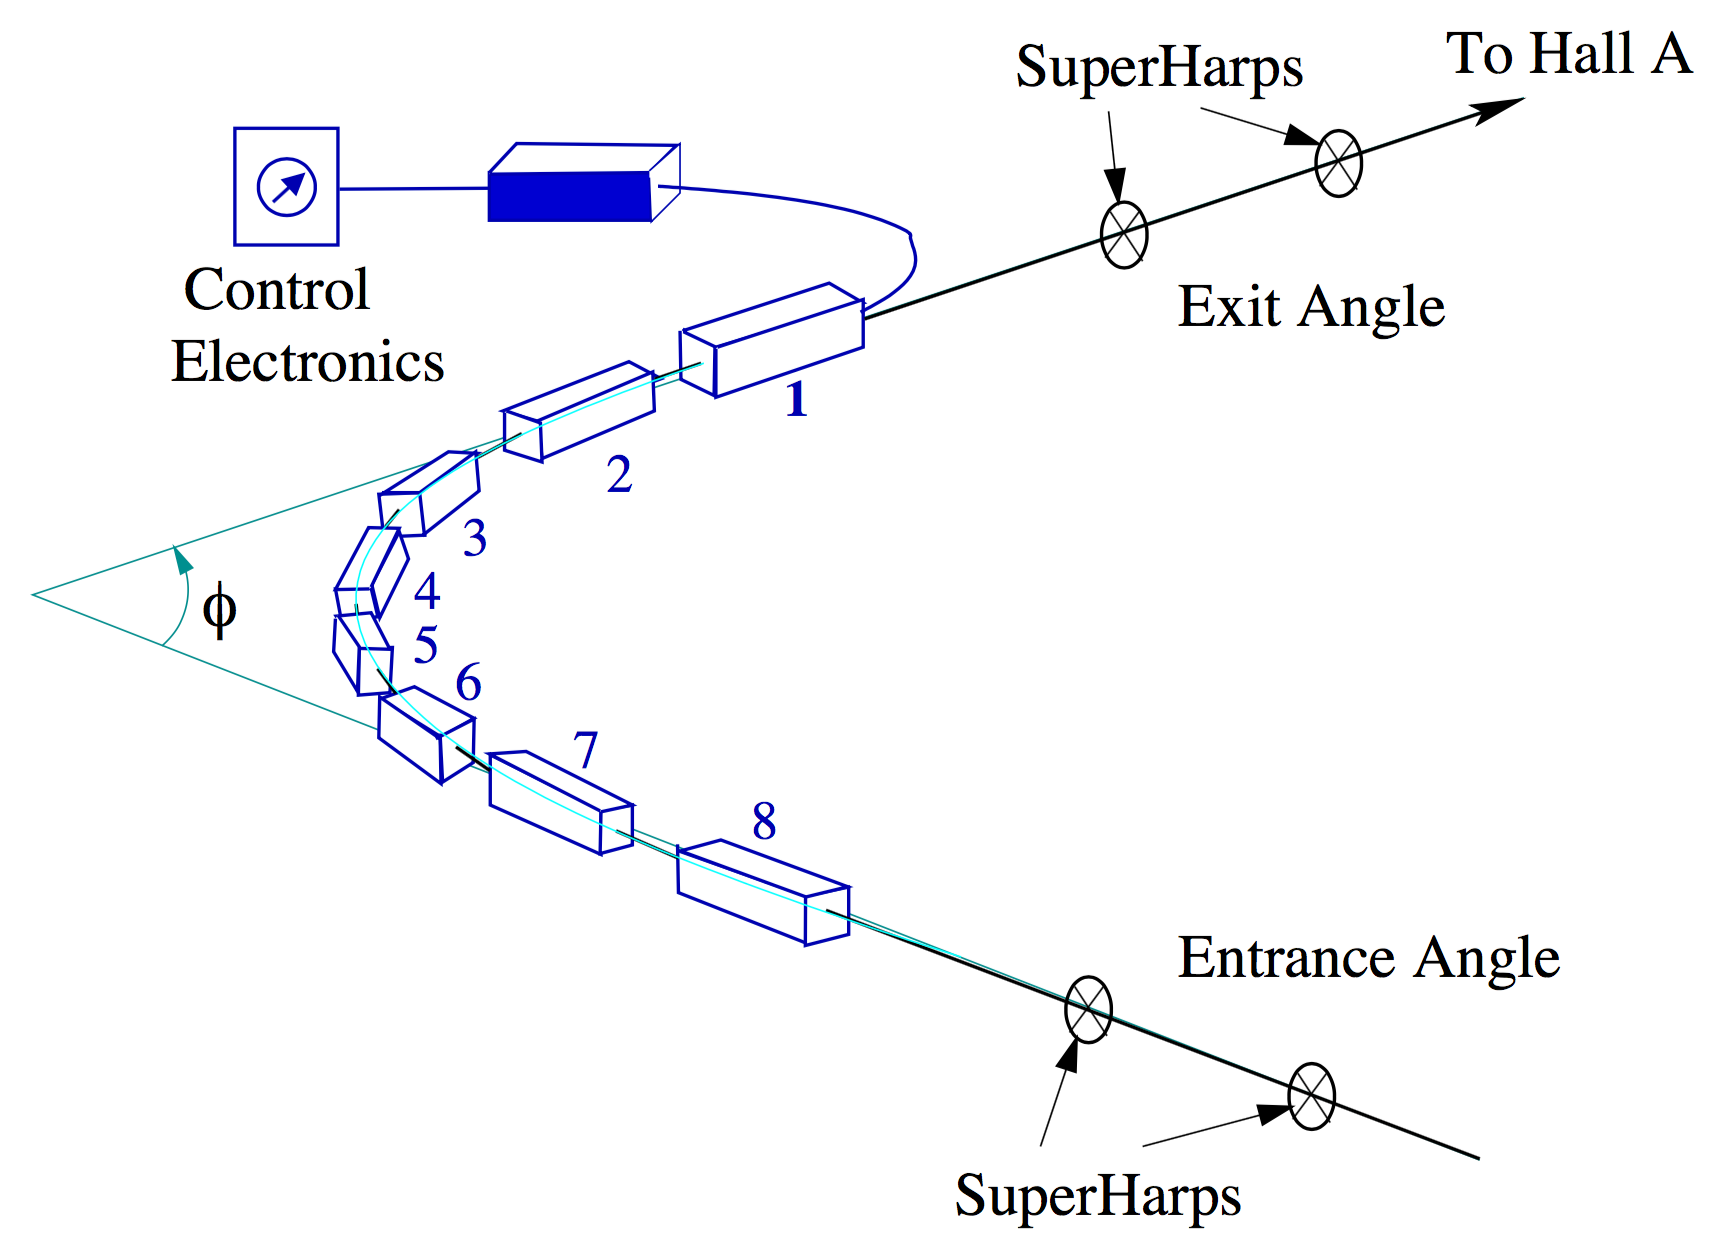
\includegraphics[width=0.6\textwidth]{figs/arc-measurement.png}
  \caption[Diagram of the arc section of the beamline.]{Diagram of the arc section of the Hall A beamline. Plot reproduced from \cite{Zheng2002}.  \label{C5S2SS1F1}}
\end{figure}

During experiment E08-027, the beam energy was measured by the Arc method \cite{Alcorn2004}. The idea of the Arc measurement is that the radius of the circular movement of an electron in a magnetic field depends on the field strength and the momentum of the electron. It measures the deflection of the beam in the arc section of the beamline, see \Cref{C5S2SS1F1}. The momentum of the beam $P$ can then be related to the integral of the magnitude of the magnetic field $B$ of the eight dipoles and the net bend angle $\theta$ through the arc sections:
\begin{equation} \label{C5S2SS1E1}
P = k \frac{\int\vec{B}\times\dd{\vec{l}}}{\theta}
\end{equation}
where $k=0.299792$ GeV$\cdot$rad$\cdot$T${}^{−1}\cdot$m${}^{−1}$/c. The Arc method relies on two simultaneous measurements. One is for the actual bend angle of the arc, and the magnetic field integral $Bdl$ of the eight dipoles in the arc based on a reference magnet measurement. The Arc energy measurement provides an absolute measurement to the $2\times10^{-4}$ GeV level.

\subsection{Beam Current Measurement}
\label{C5S2SS2}

The beam current is measured by two Beam Current Monitors (BCMs). The BCMs used in E08-027 are two stainless steel cylindrical high-$Q$ ($\sim$3000) waveguides (cavities) that are tuned to the frequency of the beam (1497 MHz) \cite{Alcorn2004}. The output voltage signals of the two cavities are proportional to the beam current. The BCM system is composed of two cavities which are located $\sim$23 m upstream from the target center, an Unser monitor and a BCM receiver which converts the raw signals to be compatible with the DAQ system.

Since the standard RMS-to-DC converter of the BCM system \cite{Denard2001} did not work at low beam current, a new BCM receiver designed by the JLab instrumentation group to improve the signal-to-noise (S/N) ratio in an environment with beam current from several nano-ampere to several micro-ampere \cite{Musson2012}. The receiver is composed of an analog part, which converts the radiofrequency (RF) signal from the cavities to the intermediate frequency (IF) signal and amplify it, and a digital part, which provides several digital filters to reduce the S/N ratio.

The RF signal with a frequency $\omega=1497$ MHz (same as beam) is mixed multiplicatively with a sinusoidal $\omega'=1452$ MHz signal from a local oscillator. Thus the mixed signal could be decomposed to a high frequency component with frequency $\omega+\omega'$ and a low frequency component with frequency $\omega-\omega'=45$ MHz. The high frequency signal is filtered out.

The 45 MHz intermediate frequency signal is amplified twice and is digitized by an analog-to-digital convertor (ADC). Two digital filters are applied to the digital signal, which can achieve higher stop-band attenuation, faster transition and higher efficiency. The cut-off frequency of the filter is set to 10.4 kHz for the BCM receiver to achieve enough S/N ratio. After the filter, the digital signal is converted back to a 0$\sim$10 V analog signal to match the input of the existed Hall A DAQ system. A voltage-to-frequency module in the DAQ system converts the voltage signal to the frequency signal and is counted by the scalers.

Usually the BCMs are calibrated with the Faraday cup in the injector. The Unser monitor located between two RF cavities could also be used to give a cross-check of the Faraday cup calibration result. However, both methods can not work at low beam currents. Therefore a tungsten calorimeter \cite{Bevins2005} was installed to calibrate our BCMs with the heating effect of the electron beam.

During the calibration, the beam is incident to the tungsten block in the calorimeter. All the electrons are stopped by the tungsten causing the temperature of the block to increase during the beam. The tungsten block is held in a vacuum chamber to minimize heat loss. The relation between the total charge and the increased temperature is:
\begin{equation} \label{C5S2SS2E1}
Q = e\cdot\frac{K_{\mathrm{W}}\cdot\Delta T}{E_{\mathrm{Beam}}},
\end{equation}
where $E_{\mathrm{Beam}}$ is the beam energy, and the $K_{\mathrm{W}}$ is the heat capacity of the tungsten. $K_{\mathrm{W}}$ of the tungsten block used in the experiment was measured before the experiment, which is 8555.5 J/K with 50 J/K uncertainty.

Once the $Q$ for a calibration run is known, the scaler readout could be calibrate via the formula:
\begin{equation} \label{C5S2SS2E2}
N = (C\cdot I+C_0)\cdot t,
\end{equation}
where $N$ is the BCM scaler reading, $C$ is the calibration constant and $C_0$ is the pedestal value of the BCM.

The uncertainty of the calibration could arise from the uncertainty of the beam energy, the temperature and the heat capacity of the tungsten as well as the effect from heat loss. The uncertainty of the beam energy measurement at Hall A is at $2\times10^{-4}$ level \cite{BEAMENERGY}. The uncertainties of the temperature sensors are 12.5 mK \cite{CALORIMETERLEDEX}. And the uncertainty of the tungsten heat capacity is 50 J/K. The Hall A calorimeter thermal and mechanical design assures that the heat losses is at $\sim$0.2\% level if the measurement takes less than 20 minutes \cite{Bevins2005}. Combining all of these effects, one could get the uncertainty of the calibration to be 0.7\%.

Since the beam current is measured by two cavities independently, the difference between the upstream and downstream BCM could be used to estimate the uncertainty of the BCM readout. The relative differences between the two BCMs are below 0.7\% for 90\% runs. See Ref. \cite{Zhu2015} for a discussion of the BCM calibration and the uncertainty estimation with more details.

\subsection{Beam Position Measurement}
\label{C5S2SS3}

Two Beam Position Monitors (BPMs) located 95.5 cm and 69.0 cm upstream from the target center were used to determine the position and direction of the beam at the target center. Each BPM contains four wire antennas parallel to the beam direction, which are placed symmetrically around the beam pipe in a vacuum chamber. When the beam passes through the BPM system, a signal is induced in each antenna. The size of each induced signal is inversely proportional to the distance from that antenna to the beam \cite{Barry1991}. \Cref{C5S2SS3F1} shows the structure of a BPM. With the assumption that the chamber is long enough so that the edge effect could be neglected and the antenna did not influence the electric field inside the chamber, the amplitude of the signal received by each antenna could be expressed as \cite{Piot2005}:
\begin{equation} \label{C5S2SS3E1}
\varphi_i = \varphi_0 I\frac{R^2-\rho^2}{R^2+\rho^2-2R\rho\cos(\theta_i-\theta_0)},
\end{equation}
where $i$ is one of four antennas $u_+$, $u_-$, $v_+$ and $v_-$, $\varphi_0$ is a constant related to the geometry of the BPM chamber and the output resistance, $I$ is the beam current, $R$ is the radius of the BPM chamber, $\rho$ is the radial position of the beam and $\theta_i-\theta_0$ is the angle difference between the antenna and the beam in a polar coordinates.

\begin{figure}[tb!]
  \centering
  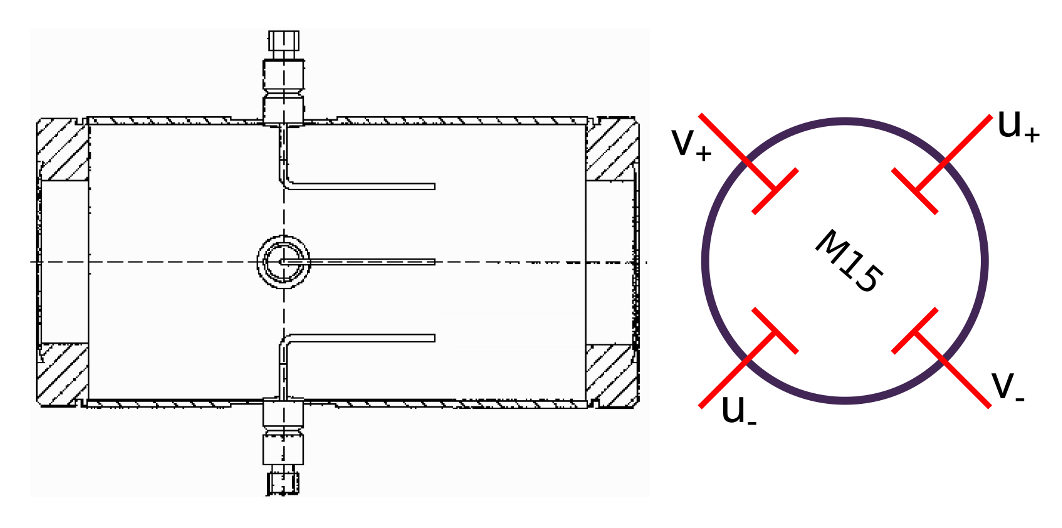
\includegraphics[width=0.7\textwidth]{figs/bpm-design.png}
  \caption[Diagram of the BPM.]{Diagram of the BPM. \label{C5S2SS3F1}}
\end{figure}

The beam position $u$ and $v$ could be extracted in the BPM local coordinates. The $u_+$ and $u_-$ antennas define the $\hat{u}$ axis of this coordinate system and the $v_+$ and $v_-$ antennas define the $\hat{v}$ axis. If $u^2+v^2\ll R^2$, the beam position can be expressed as:
\begin{equation} \label{C5S2SS3E2}
W \approx \frac{R}{2}D_W,
\end{equation}
with
\begin{equation} \label{C5S2SS3E3}
D_W= \frac{R}{2}\frac{\varphi_{W_+}-\varphi_{W_-}}{\varphi_{W_+}+\varphi_{W_-}}.
\end{equation}
Here $W$ denotes $u$ and $v$. Since the beam is circularly rastered with a diameter of 2 cm in E08-027, \cref{C5S2SS3E2} is no longer valid, and the beam position can be calculated via a corrected formula:
\begin{equation} \label{C5S2SS3E4}
W = RD_W\left(\frac{1}{D^2}-\frac{1}{D}\sqrt{\frac{1}{D^2}-1}\right),
\end{equation}
with $D^2=D_u^2+D_v^2$.

Like the BCMs, the BPM system also contains a receiver which collects and sends the signal to the DAQ system. As mentioned in \Cref{C5S2SS3}, the original receiver did not work at low beam currents, thus a new BPM receiver was designed by the JLab instrumentation group \cite{Musson2012} to be compatible with beam current as low as 50 nA. The output signal of the receiver is sent to a 13-bit fastbus ADC with an integration time of 50 ns which is triggered by a detected event. The BPM receiver shares the same design with the BCM receiver, but the cut-off frequency of the digital filter of the BPM receiver is set to 175 Hz to increase the S/N ratio and reach the required resolution. This leads to a 1/175 s delay of the beam position signal. There is also a $\sim$4 $\mu$s delay as the processing time of the electronics. Since the beam is spread by a 25 kHz fast raster, the BPM could not provide the beam position event by event due to the time delay effect.

\begin{figure}[b!]
  \centering
  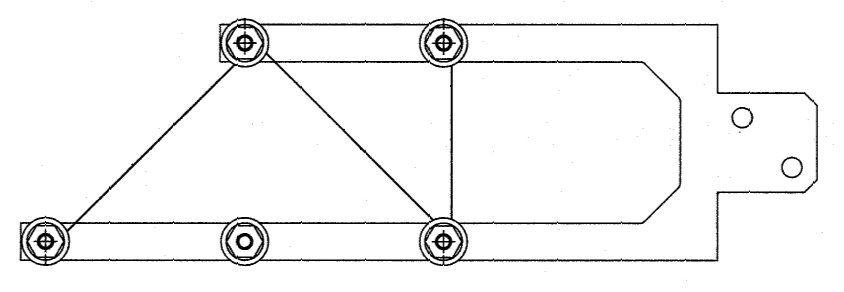
\includegraphics[width=0.5\textwidth]{figs/harp.png}
  \caption[Diagram of the harp.]{Diagram of the harp. \label{C5S2SS3F2}}
\end{figure}

The BPMs are calibrated with two superharps. One harp is installed between the 2 BPMs and the other one is installed upstream of the upstream chicane magnet. \Cref{C5S2SS3F2} shows a schematic diagram of the harp. The harp consists of three wires with a thickness of 50 $\mu$m which are fixed to a chassis controlled by a step motor \cite{Yan1995}. The original position of each wire is surveyed with a precision level of 0.1 mm. During the calibration, the harp is moved into the beam pipe by the step motor. The wires are scanned by the electron beam resulting showers of particles which can be detected. The absolute beam position could be calculated with the recorded wire signal and the survey result. Meanwhile the beam position is also measured with BPMs. By comparing the readout and the wire signal, the BPMs can be calibrated.

The BPMs only measure the beam position at their own locations. Usually the beam positions at BPMs could be linear projected to the target location to retrieve the beam positions at the target. However, the transverse target field in E08-027 breaks the linear projection. A simulation package was constructed to trace the movement of the incident electrons in the target field. The beam trajectories generated by the simulation package are used to fit a set of transport functions which could transport the beam positions at two BPMs to the spatial coordinates and the incident angles of the beam at the target location. These transport functions are used to calculate the beam position at the target location.

As mentioned above, the BPM could not provide the beam position event by event if the beam is rastered. Thus the raster information is combined with the BPM readout to provide the beam position for each event. Here the BPM is only used to measure the center of the raster pattern. The magnet current of the rasters is calibrated to get the absolute values of the deviations with respect to the center of the raster pattern. The details of the rasters used in the experiment will be discussed in \Cref{C5S2SS5}.

The uncertainty of the final beam position at the target location arises from several sources such as the uncertainty of the harp calibration constant, the survey data and the pedestal value of the electronics. The final uncertainty of the beam positions is 1$\sim$2 mm, while the uncertainty of the incident angles is 1$\sim$2 mrad. See Ref. \cite{Zhu2014} for a detailed discussion of the BCM calibration and the uncertainty estimation with more details.

\subsection{Beam Polarization}
\label{C5S2SS4}

The polarization of the electron beam was measured by the M{\o}ller polarimeter during E08-027. The polarimeter uses polarized M{\o}ller scattering, in which polarized electron beam scatters off polarized atomic electrons in a magnetized ferromagnetic foil $\vec{e}\,^-+\vec{e}\,^-\rightarrow e^-+e^-$, to measure the beam polarization \cite{MOLLER,Alcorn2004}. The coordinate system is defined such that the beam direction is along the $z$-axis and the $y$-axis is perpendicular to the scattering plane. The M{\o}ller scattering cross-section can be expressed in terms of the beam polarization $P_{\mathrm{beam}}^i$ and target polarization $P_{\mathrm{target}}^i$ \cite{Alcorn2004}:
\begin{equation} \label{C5S2SS4E1}
\sigma = \sigma_0\left[1+\sum_{i=x,y,z}A_{ii}P_{\mathrm{beam}}^iP_{\mathrm{target}}^i\right],
\end{equation}
where $i$ is the projection direction of the polarization, and $\sigma_0$ is the unpolarized M{\o}ller cross-section. The $A_{ii}$ are the analyzing powers which can be expressed as:
\begin{align} \label{C5S2SS4E2}
A_{zz} & = -\frac{\sin^2\theta_{\mathrm{cm}}\cdot(7+\cos^2\theta_{\mathrm{cm}})}{(3+\cos^2\theta_{\mathrm{cm}})^2}, \\ \label{C5S2SS4E3}
A_{xx} & = -A_{yy} =  -\frac{\sin^4\theta_{\mathrm{cm}}}{(3+\cos^2\theta_{\mathrm{cm}})^2}.
\end{align}
Since the beam is longitudinal polarized, the corresponding analyzing power is $A_{zz}$, which reaches its maximum value of $7/9$ when $\theta_{\mathrm{cm}}=$\SI{90}{\degree}. The polarized M{\o}ller cross-sections are less sensitive to the transverse polarization and the data with opposite target transverse polarization could be averaged to cancel the transverse contributions.

\begin{figure}[b!]
  \centering
  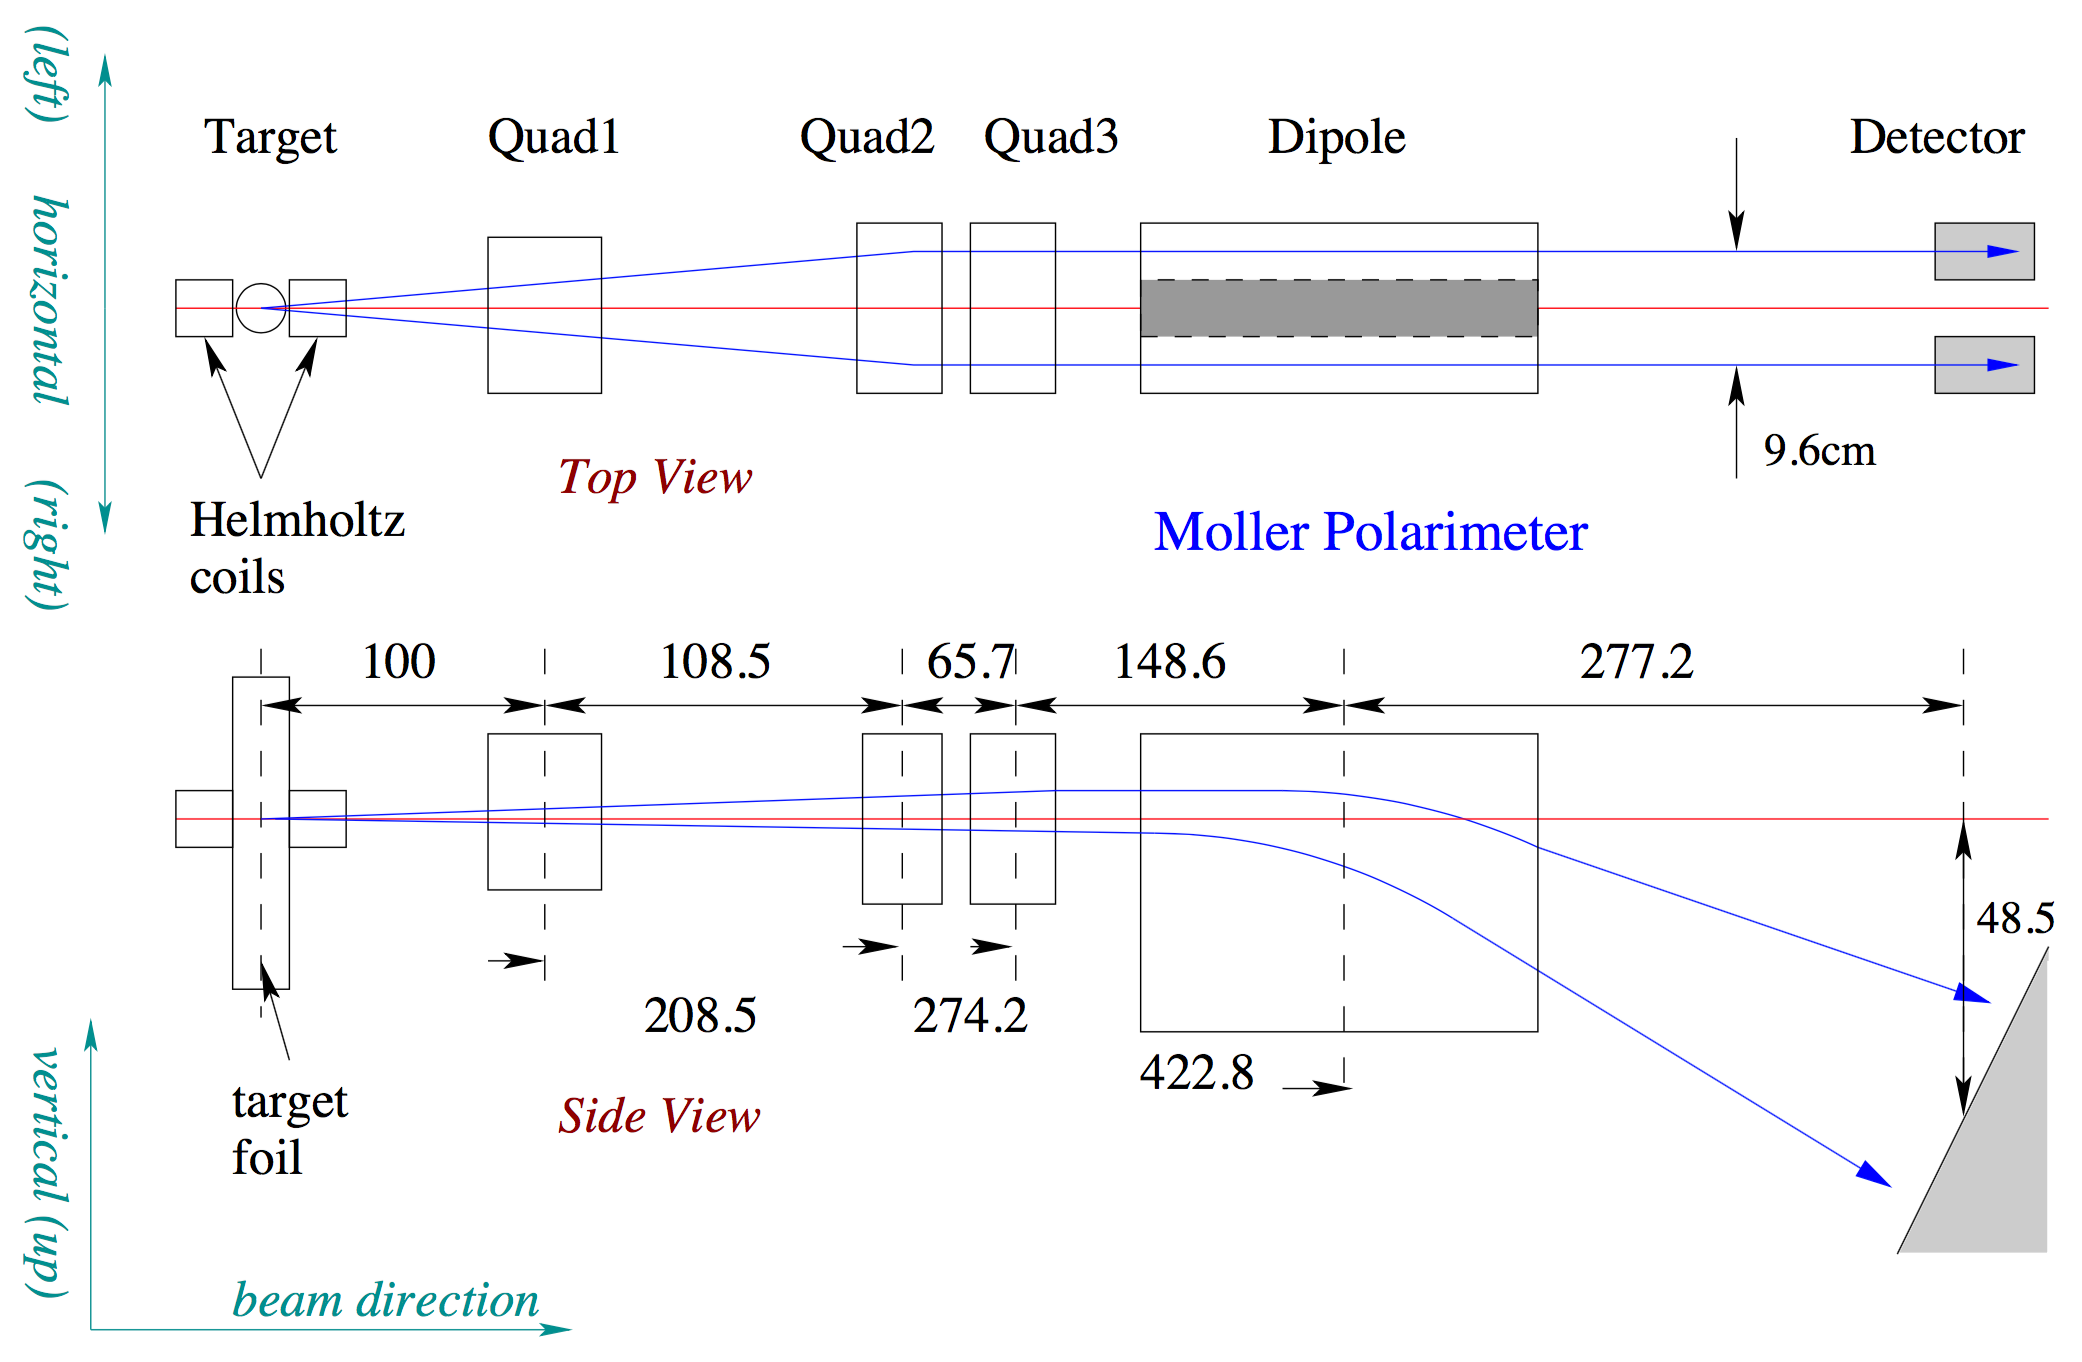
\includegraphics[width=\textwidth]{figs/moller.png}
  \caption[Schematic diagram of the M{\o}ller polarimeter.]{Schematic diagram of the M{\o}ller polarimeter. Plot reproduced from \cite{Zheng2002}. \label{C5S2SS4F1}}
\end{figure}

During the experiment, a pair of asymmetries are measured at two target angles of about $\pm$\SI{20}{\degree} with respect to the beam in the horizontal plane, and the average is taken to cancel the transverse contributions as mentioned above. Here asymmetries are measured rather than cross-sections since the asymmetry is a ratio of cross-sections, thus most of the systematic uncertainties related to the cross-section measurement cancel out when taking the ratio. \Cref{C5S2SS4F1} shows a sketch of the M{\o}ller polarimeter. The polarimeter is composed of three quadrupoles and a dipole. The detector system consists of scintillators and lead-glass calorimeter modules. The statistical accuracy is typically 0.2\% as discussed in Ref. \cite{Alcorn2004}. There is a $\sim$3\% relative systematic uncertainty dominated by the knowledge of the foil polarization.

The beam longitudinal polarization is measured as:
\begin{equation} \label{C5S2SS4E4}
P_{\mathrm{beam}} = \frac{1}{P_{\mathrm{target}}\cos\theta_{\mathrm{target}}\expval{A_{zz}}}\times\frac{N_+-N_-}{N_+-N_-},
\end{equation}
where $N_+$ and $N_-$ are the detected events with opposite orientations of beam polarization. The average analyzing power $\expval{A_{zz}}$ is  calculated with a Monte-Carlo simultion of the M{\o}ller polarimeter. Nine measurements were taken during the experiment, which were scheduled during beam unavailable periods or during a configuration change in the accelerator. The M{\o}ller measurement results are shown in \cref{C5S2SS4T1}.

\begin{table}[h!]
  \centering
  \newcolumntype{C}[1]{>{\centering\arraybackslash}m{#1}}
  \begin{tabular}{|c|c|C{2.5cm}|C{2.5cm}|}
    \hline
      & Date & Polarization (\%) & Systematic Error (\%) \\ \hline
    1 & 03/03/2012 & 79.91$\pm$0.20 & $\pm$1.7 \\ \hline
    2 & 03/30/2012 & 80.43$\pm$0.46 & $\pm$1.7 \\ \hline
    3 & 03/30/2012 & 79.89$\pm$0.58 & $\pm$1.7 \\ \hline
    4 & 04/10/2012 & 88.52$\pm$0.30 & $\pm$1.7 \\ \hline
    5 & 04/23/2012 & 89.72$\pm$0.29 & $\pm$1.7 \\ \hline
    6 & 05/04/2012 & 83.47$\pm$0.57 & $\pm$1.7 \\ \hline
    7 & 05/04/2012 & 81.82$\pm$0.59 & $\pm$1.7 \\ \hline
    8 & 05/04/2012 & 80.40$\pm$0.45 & $\pm$1.7 \\ \hline
    9 & 05/15/2012 & 83.59$\pm$0.31 & $\pm$1.7 \\ \hline
  \end{tabular}
  \caption[Beam energy and target field configurations.]{Summary of the M{\o}ller measurement result. Table reproduced from \cite{MOLLERG2P}. \label{C5S2SS4T1}}
\end{table}

\subsection{New Instruments}
\label{C5S2SS5}

\subsubsection{Raster System}

The polarized target was operated at $\sim$1 K, it would depolarize if the target material was heated by the electron beam. Thus the beam position was rastered to avoid localized overheating the target material. A uniform distribution of beam on the target is achieved by moving the beam position with time-varying dipole magnetic fields. These dipoles were referred to as rasters.

Two raster systems, the fast raster and the slow raster, were installed at $\sim$17 m upstream from the target center. The fast raster is a standard Hall A beamline component, which consists of two dipole magnets. Both of the dipoles were driven by the same current in a triangular waveform with frequency of 25 kHz. The beam position moved by the dipole fields in $\hat{x}$ and $\hat{y}$ directions respectively and formed a 2 mm $\times$ 2 mm rectangular pattern. The shape of the fast raster pattern is shown in \Cref{C5S2SS5F1}.

\begin{figure}[b!]
  \centering
  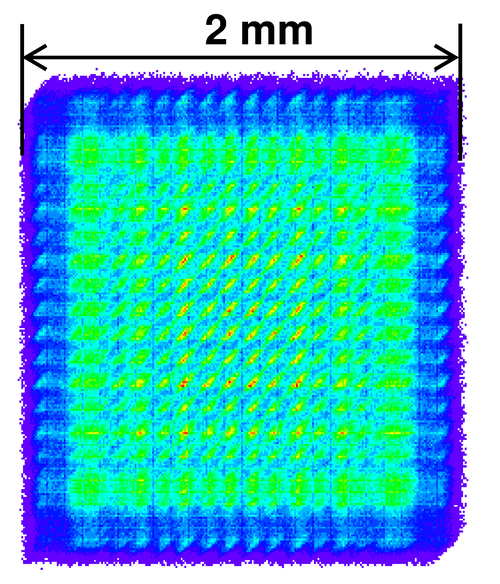
\includegraphics[width=0.2\textwidth]{figs/fast-raster-pattern.png}
  \caption[Fast raster pattern.]{Fast raster pattern. The plot is produced from the magnet current signal. \label{C5S2SS5F1}}
\end{figure}

The target cell of the E08-027 experiment is a cylinder with $\sim$25 mm diameter. Thus the fast raster is not enough to spread the beam uniformly on to the whole target. A slow raster was installed in Hall A right downstream to the fast raster. The slow raster also consists of two dipole magnets, however the driven current of the dipoles is not in triangular waveform. The waveform used in the slow raster could spread the beam to a circle with $\sim$20 mm diameter. A dual-channel function-generator was used to generate two independent waveforms to drive the dipole magnet of the slow raster. The waveforms for $x$ and $y$ directions are:
\begin{align} \label{C5S2SS5E1}
I_x & = I_x^{\mathrm{max}}f(t^{\frac{1}{2}})\sin(\omega t), \\ \label{C5S2SS5E2}
I_y & = I_y^{\mathrm{max}}f([t+t_0]^{\frac{1}{2}})\cos(\omega t),
\end{align}
where the $I_x^{\mathrm{max}}$ and $I_y^{\mathrm{max}}$ are the maximum amplitude. They are actually the parametric equations of a circle which is modulated by a function $f(t^{\frac{1}{2}})$ to generate a uniform circular pattern \cite{Yan2005}. The amplitude modulation (AM) function $f(t^{\frac{1}{2}})$ is a periodic piecewise function with frequency $1/T$. $f(t^{\frac{1}{2}})$ can be expressed as (in the first period):
\begin{equation} \label{C5S2SS5E3}
f(t) =
\begin{cases}
t^{\frac{1}{2}}, & \text{if } 0\leq t<T/4, \\
(T/2-t)^{\frac{1}{2}}, & \text{if } T/4\leq t<T/2, \\
-(t-T/2)^{\frac{1}{2}}, & \text{if } T/2\leq t<3T/4, \\
-(T-t)^{\frac{1}{2}}, & \text{if } 3T/4\leq t<T.
\end{cases}
\end{equation}
The $t_0$ in \cref{C5S2SS5E1} is the phase difference between the AM functions of $\hat{x}$ and $\hat{y}$ direction.

\begin{figure}[tb!]
  \centering
  \begin{subfigure}[t]{0.2\textwidth}
    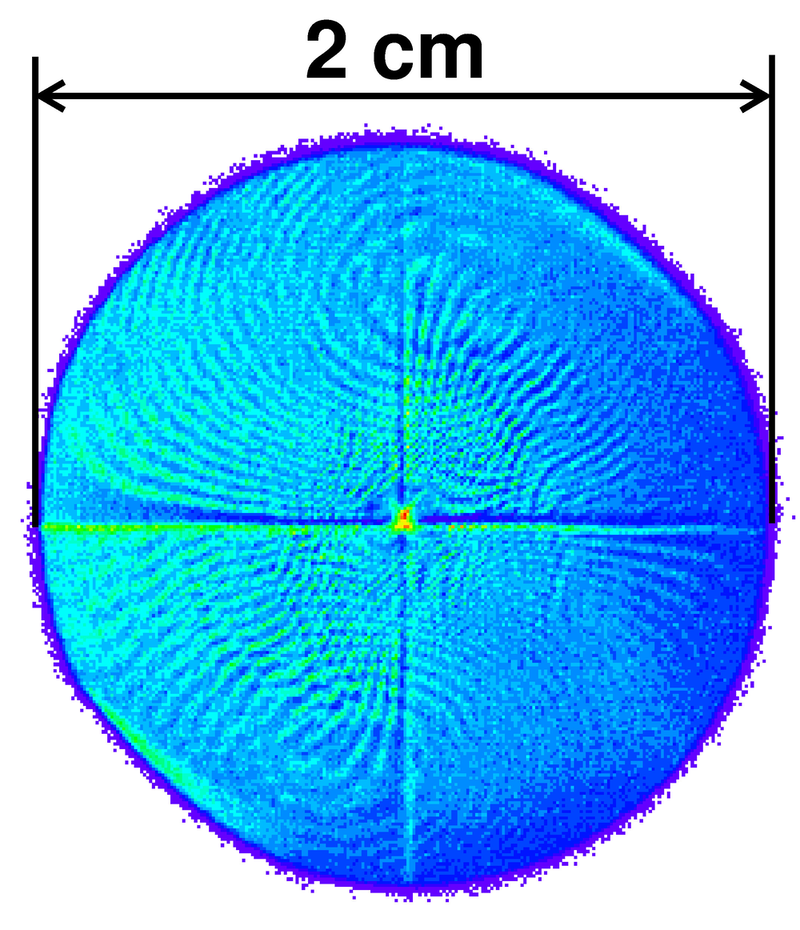
\includegraphics[width=\textwidth]{figs/slow-raster-pattern.png}
    \caption{Slow raster magnet current distribution. \label{C5S2SS5F2a}}
  \end{subfigure}
  \qquad
  \begin{subfigure}[t]{0.2\textwidth}
    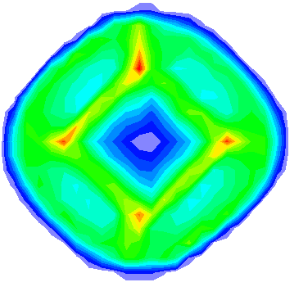
\includegraphics[width=\textwidth]{figs/slow-raster-pattern-data-bad.png}
    \caption{Slow raster pattern with $t_0\neq0$. \label{C5S2SS5F2b}}
  \end{subfigure}
  \qquad
  \begin{subfigure}[t]{0.2\textwidth}
    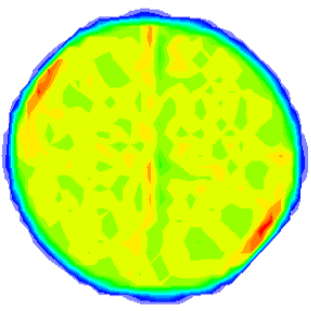
\includegraphics[width=\textwidth]{figs/slow-raster-pattern-data-good.png}
    \caption{Slow raster pattern with $t_0=0$. \label{C5S2SS5F2c}}
  \end{subfigure}
  \caption[Slow raster pattern.]{Slow raster pattern. Here (b) and (c) are produced from the BPM readout.  \label{C5S2SS5F2}}
\end{figure}

During the experiment E08-027, the frequency $\omega$ of the sine pattern in the waveforms was 99.412 Hz. The frequency $1/T$ of the AM function was set to 30 Hz. The phase difference $t_0$ was manually adjusted to be 0. A non-zero $t_0$ could cause a non-uniform pattern as shown in \Cref{C5S2SS5F2b}. Thus, $t_0$ was carefully minimized during the experiment to avoid the non-uniformity. The pattern of the beam was relatively uniform after the adjustment as shown in \Cref{C5S2SS5F2c}.

\subsubsection{Chicane Magnets}

The strong transverse magnetic field in the target region influences the electron beam. The direction of the magnetic field was pointing to the left of the beam if looking along the downstream direction. According to the right-hand rule, the electron beam would be deflected downwards in the target field. Two chicane magnets were placed in front of the target and the BPMs to provide an upward incident angle for the electron beam when it reaches the center of the target. \Cref{C5S2SS5F3} shows the effects of the chicane magnets and the target field on the electron beam. The first chicane magnet was installed 5.92 m upstream from the target center would bend the beam downwards. The second chicane magnet, which was installed 2.66 m upstream from the target center, would bend the beam back towards the target. The vertical position of the chicane magnets was adjusted according to the beam energy and the target field configuration during the experiment.

\begin{figure}[b!]
  \centering
  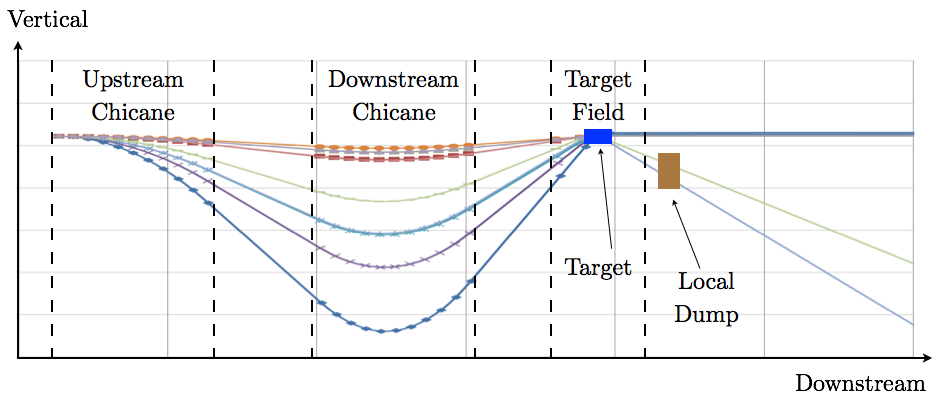
\includegraphics[width=0.9\textwidth]{figs/beam-traj.png}
  \caption[Schematic diagram of the effects of the chicane magnets.]{Schematic diagram of the effects of the chicane magnets and the target field on the electron beam. The trajectories are marked with different colors for different beam energy and target field configuration. Notice the diagram does not reflect the actual scale of each component. \label{C5S2SS5F3}}
\end{figure}

\subsubsection{Local Beam Dump}

As seen in \Cref{C5S2SS5F3}, most of the beam trajectories exit the target field region horizontally (in these cases the target field strength is 2.5 T), and could reach the Hall A beam dump. However, the chicane magnets could not bend the beam to the Hall A beam dump for those configurations with the 5.0 T transverse target field. Since the beam current was quite low for this experiment, a local beam dump which consisted of a series of tungsten and copper plates could be used to stop the beams which could not reach the Hall A beam dump. The local beam dump was installed downstream of the polarized target as shown in \Cref{C5S2SS5F3}. The local beam dump worked well during the experiment and successfully protected the electronics in the experimental hall from high background radiation.

\section{\texorpdfstring{Polarized NH${}_3$ Target}{Polarized NH3 Target}}
\label{C5S3}

In experiment E08-027, a polarized ammonia target was used to provide an effective proton target since the nucleons in the Nitrogen nuclei are not coupled with the electrons thus they would not be polarized by the Dynamic Nuclear Polarization (DNP) method. This target has been successfully used for several JLab experiments prior to E08-027. The target has demonstrated a high polarization up to 90\% with a 5.0 T target field. The 5.0 T target field was used in E08-027 and a new 2.5 T configuration was operated in this experiment for the first time.

\subsection{Dynamic Nuclear Polarization}
\label{C5S3SS1}

The DNP method is used to polarize the hydrogen nuclei in a NH${}_3$ target. Zeeman effect tells us that a spin non-zero particle located in a strong magnetic field is polarized spontaneously. If the magnetic moment of the particle is $\mu$ and the spin is 1/2, the ground state of this particle split to two sublevels with energy $E_0+\mu B$ and $E_0-\mu B$ respectively. The population of these two sublevels follows Maxwell-Boltzmann statistics:
\begin{equation} \label{C5S3SS1E1}
N(E_0\pm\mu B) = N(E_0)\exp(-\frac{\pm\mu B}{k_B T}),
\end{equation}
where $k_B$ is the Boltzmann constant and $T$ is the temperature of the system. Thus the spontaneous polarization of the material is:
\begin{equation} \label{C5S3SS1E2}
P_{\mathrm{TE}} = \frac{\exp(\frac{\mu B}{k_BT})-\exp(-\frac{\mu B}{k_BT})}{\exp(\frac{\mu B}{k_BT})+\exp(-\frac{\mu B}{k_BT})} = \tanh(\frac{\mu B}{k_B T}).
\end{equation}
We also refer to this polarization as the thermal polarization. The thermal polarization of a sample of electrons is above 90\% but the proton's thermal polarization is only $\sim$2.5\% for 1 K temperature and 2.5 T magnetic field which is a typical target configuration in E08-027.

\begin{figure}[b!]
  \centering
  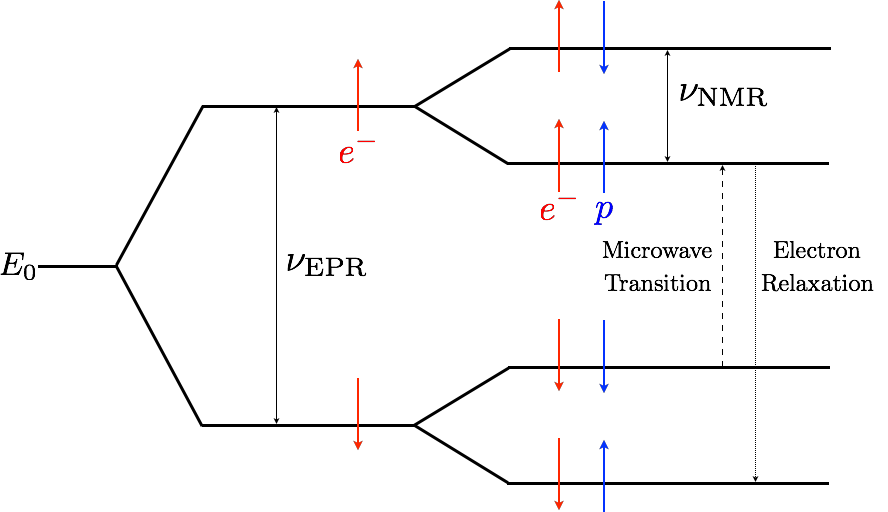
\includegraphics[width=0.6\textwidth]{figs/DNP.png}
  \caption[Electron-proton spin coupling interaction diagram.]{Electron-proton spin coupling interaction diagram. \label{C5S3SS1F1}}
\end{figure}

The thermal polarization is not enough to polarize the protons in the target. Thus the DNP method is developed to enhance the polarization by transferring the electron polarization to the nucleon via the electron-proton spin coupling \cite{Overhauser1953,Jeffries1957}. The Hamiltonian of this system can be written as:
\begin{equation} \label{C5S3SS1E3}
H = \vec{\mu_e}\cdot\vec{B}+\vec{\mu_p}\cdot\vec{B}+H_{\mathrm{ss}},
\end{equation}
where the $H_{ss}$ arises from the interaction of the electron and proton. The ground state of this system split to four sublevels as shown in \Cref{C5S3SS1F1}. A microwave generator can be used to flip the proton spin and electron spin together if the frequency is carefully tuned at $\nu_{\mathrm{EPR}}-\nu_{\mathrm{NMR}}$ to polarize the proton in the field direction (or $\nu_{\mathrm{EPR}}+\nu_{\mathrm{NMR}}$ for an opposite direction). Here the $\nu_{\mathrm{EPR}}$ is the electron paramagnetic resonance (EPR) frequency and $\nu_{\mathrm{NMR}}$ is the proton nuclear magnetic resonance (NMR) frequency. Since the relaxation time of electrons is only a few milliseconds, the polarized electron is relaxed and can be used to polarize a new proton. The relaxation time of proton is tens of minutes so the polarization of proton could be kept if we pump with the microwave continuously.

\subsection{Target Setup}
\label{C5S3SS2}

\begin{figure}[b!]
  \centering
  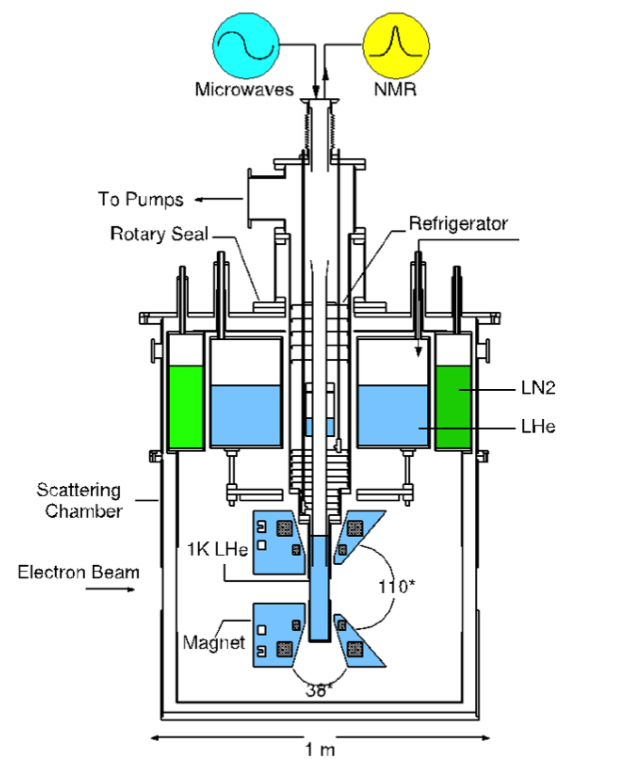
\includegraphics[width=0.6\textwidth]{figs/target.png}
  \caption[Diagram of the polarized NH${}_3$ target system.]{Diagram of the polarized NH${}_3$ target system. \label{C5S3SS2F1}}
\end{figure}

The NH${}_3$ target system used in E08-027 is shown in \Cref{C5S3SS2F1}. The original 5 T oxford superconducting magnet was burned before the experiment. Fortunately, an alternate magnet from Hall B was identified as a suitable replacement. Because of the power and construction limit of the chicane magnets, a 2.5 T field configuration was used in addition to the original 5.0 T magnetic field to reach the minimum possible $Q^2$ with this magnet. The magnetic field must be uniform in order for the DNP process to be efficient. The nonuniformity of the field is less than $10^{−4}$ over the volume of the material which is a cylinder with $\sim$2 cm diameter and $\sim$2 cm length \cite{Pierce2014}. The open geometry of the magnet allows the beam to pass through in both longitudinal and transverse configurations. The magnet is superconducting and is maintained at 4 K with a reservoir of liquid helium.

The target stick can be seen in \Cref{C5S3SS2F2}. The stick contains two NH${}_3$ cells, a carbon foil cell, a ``dummy'' cell and two small disk targets made with carbon and polyethylene respectively. The NH${}_3$ cells are filled with solid NH${}_3$ beads and are covered with aluminum foils. A short Cu-Ni capillary coil is installed in the cell for NMR measurement. The dummy cell is identical to the NH${}_3$ cells which also includes aluminum foils and the NMR coil, but does not contain any NH${}_3$ beads. During the experiment, the end of the target stick is immersed in a container full of liquid helium, which is refered as the target ``nose''. A ${}^4$He evaporation refrigerator was used to cool down the target and maintain its temperature at 1.1 K with 3 W microwave power \cite{Pierce2014}.

\begin{figure}[tb!]
  \centering
  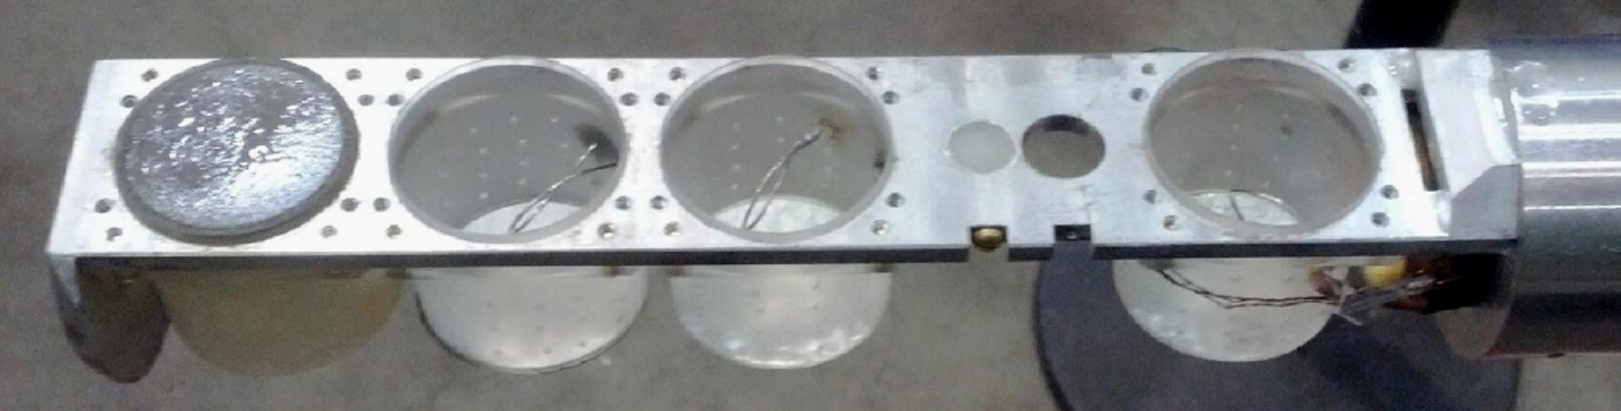
\includegraphics[width=0.6\textwidth]{figs/target-insert.png}
  \caption[The end of the target insert.]{The end of the target insert. A carbon foil cell, a ``dummy'' cell and two NH${}_3$ cells are installed in the stick from left to right. And a carbon disk and a polyethylene disk are installed in the holes between two NH${}_3$ cells. \label{C5S3SS2F2}}
\end{figure}

The selection of NH${}_3$ as the target material is due to several reasons. It has been proved that NH${}_3$ is capable of reaching 90\% polarization in a 5 T magnetic field. And it can be polarized within 30 minutes or less, which is very fast compare to other materials. Solid NH${}_3$ also holds up very well against radiation damage which could reduce the polarization rapidly. The radiation can produce additional radicals that reduce the relaxation time of the proton. The beam current is limited to 50 nA during the experiment to reduce the radiation damage, however the NH${}_3$ beads still need to be replaced several times during the experiment.

\begin{figure}[tb!]
  \centering
  \begin{subfigure}[t]{0.2\textwidth}
    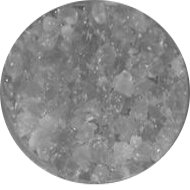
\includegraphics[width=\textwidth]{figs/ammonia-unirradiated.jpg}
    \caption{Unirradiated. \label{C5S3SS2F3a}}
  \end{subfigure}
  \qquad
  \begin{subfigure}[t]{0.2\textwidth}
    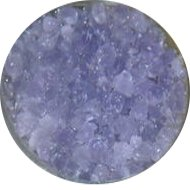
\includegraphics[width=\textwidth]{figs/ammonia-irradiated.jpg}
    \caption{Irradiated. \label{C5S3SS2F3b}}
  \end{subfigure}
  \caption[NH${}_3$ beads before and after irradiation.]{NH${}_3$ beads before and after irradiation. \label{C5S3SS2F3}}
\end{figure}

However, radicals in the target material can also allow the material to polarize faster. The NH${}_3$ beads are irradiated with a 10 MeV linear accelerator at National Institute of Standards and Technology (NIST) before the experiment in order to produce a few additional radicals in the material. The irradiation causes the solid NH${}_3$ beads to become a deep purple color, as seen in \Cref{C5S3SS2F3}. The number of radicals in the material must be carefully balanced: they can speed up the DNP process, but they also increase the speed of the proton depolarization. The DNP process becomes inefficient when the target is exposed in the electron beam long enough with the amount of radicals exceeding the tolerance. To counteract this effect, the target material is heated up to force the radicals to recombine, which is referred to as the ``annealing'' of the target. There is a limit to how many times the material can be annealed. thus the material need to be replaced at some point.

Microwaves are necessary to drive the spin transitions. The microwave generator contains an Extended Interaction Oscillator (EIO) tube to generate the microwave. The microwaves are then carried via waveguides to a horn close to the target cell. The optimal frequency of the microwave radiation is not a constant value due to the radiation damage. Thus the frequency need to be tweaked throughout the experiment.

\subsection{Target Polarization Measurement}
\label{C5S3SS3}

The polarization is measured via the NMR method. An LCR circuit with resonance frequency equal to the Larmor frequency of the proton is used as the NMR circuit \cite{Crabb1997}. The power lost or gained in the circuit can be measured via the quality factor ($Q$-factor) of the circuit by a $Q$-meter. The response of the target material to a radiofrequency irradiation is described by its magnetic susceptibility $\chi(\omega)=\chi'(\omega)-i\chi''(\omega)$, where $\chi'(\omega)$ and $\chi''(\omega)$ are the dispersive and absorptive part of the susceptibility respectively. The polarization $P$ of the target is related to the absorptive part of the susceptibility $\chi(\omega)$ \cite{Goldman1975}:
\begin{equation} \label{C5S3SS3E1}
P = K\int_0^\infty\chi''(\omega)\dd{\omega},
\end{equation}
where $K$ is a constant containing the properties of the NMR system. The NMR circuit has inductance $L_C$ and resistance $r_C$ itself, and the inductive coupling between the material and the coil changes the impedance of the circuit to:
\begin{equation} \label{C5S3SS3E2}
Z_C = r_C+i\omega L_C(1+4\pi\eta\chi(\omega)),
\end{equation}
where $\eta$ is the filling factor of the coil. The circuit is driven by an RF generator which sweeps through a range of frequencies around the Larmor resonance of the circuit.


\begin{figure}[p!]
  \centering
  \begin{subfigure}[t]{0.49\textwidth}
    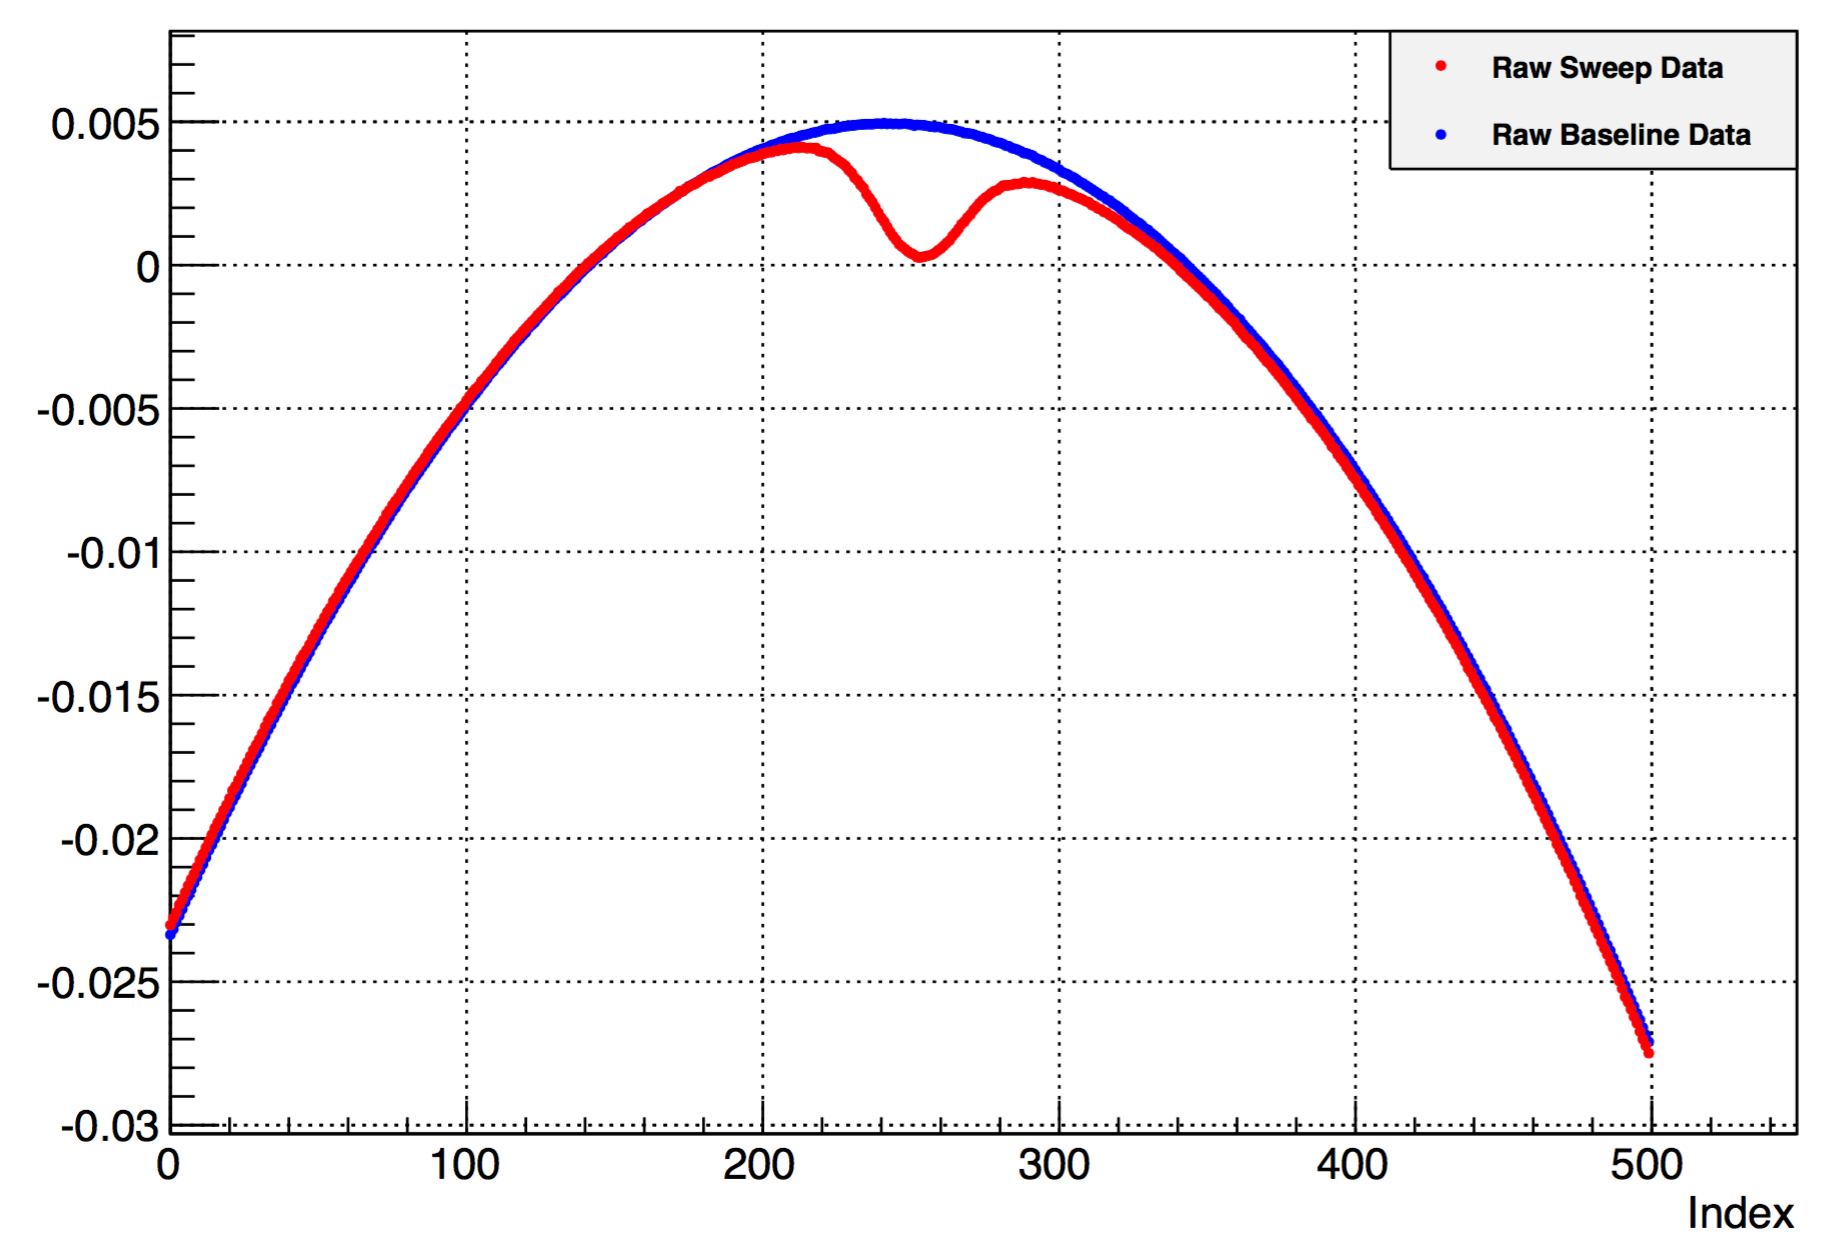
\includegraphics[width=\textwidth]{figs/target-NMR-raw.png}
    \caption{The raw signal (red) and the baseline signal ($Q$-curve signal, blue). \label{C5S3SS3F1a}}
  \end{subfigure}
  \begin{subfigure}[t]{0.49\textwidth}
    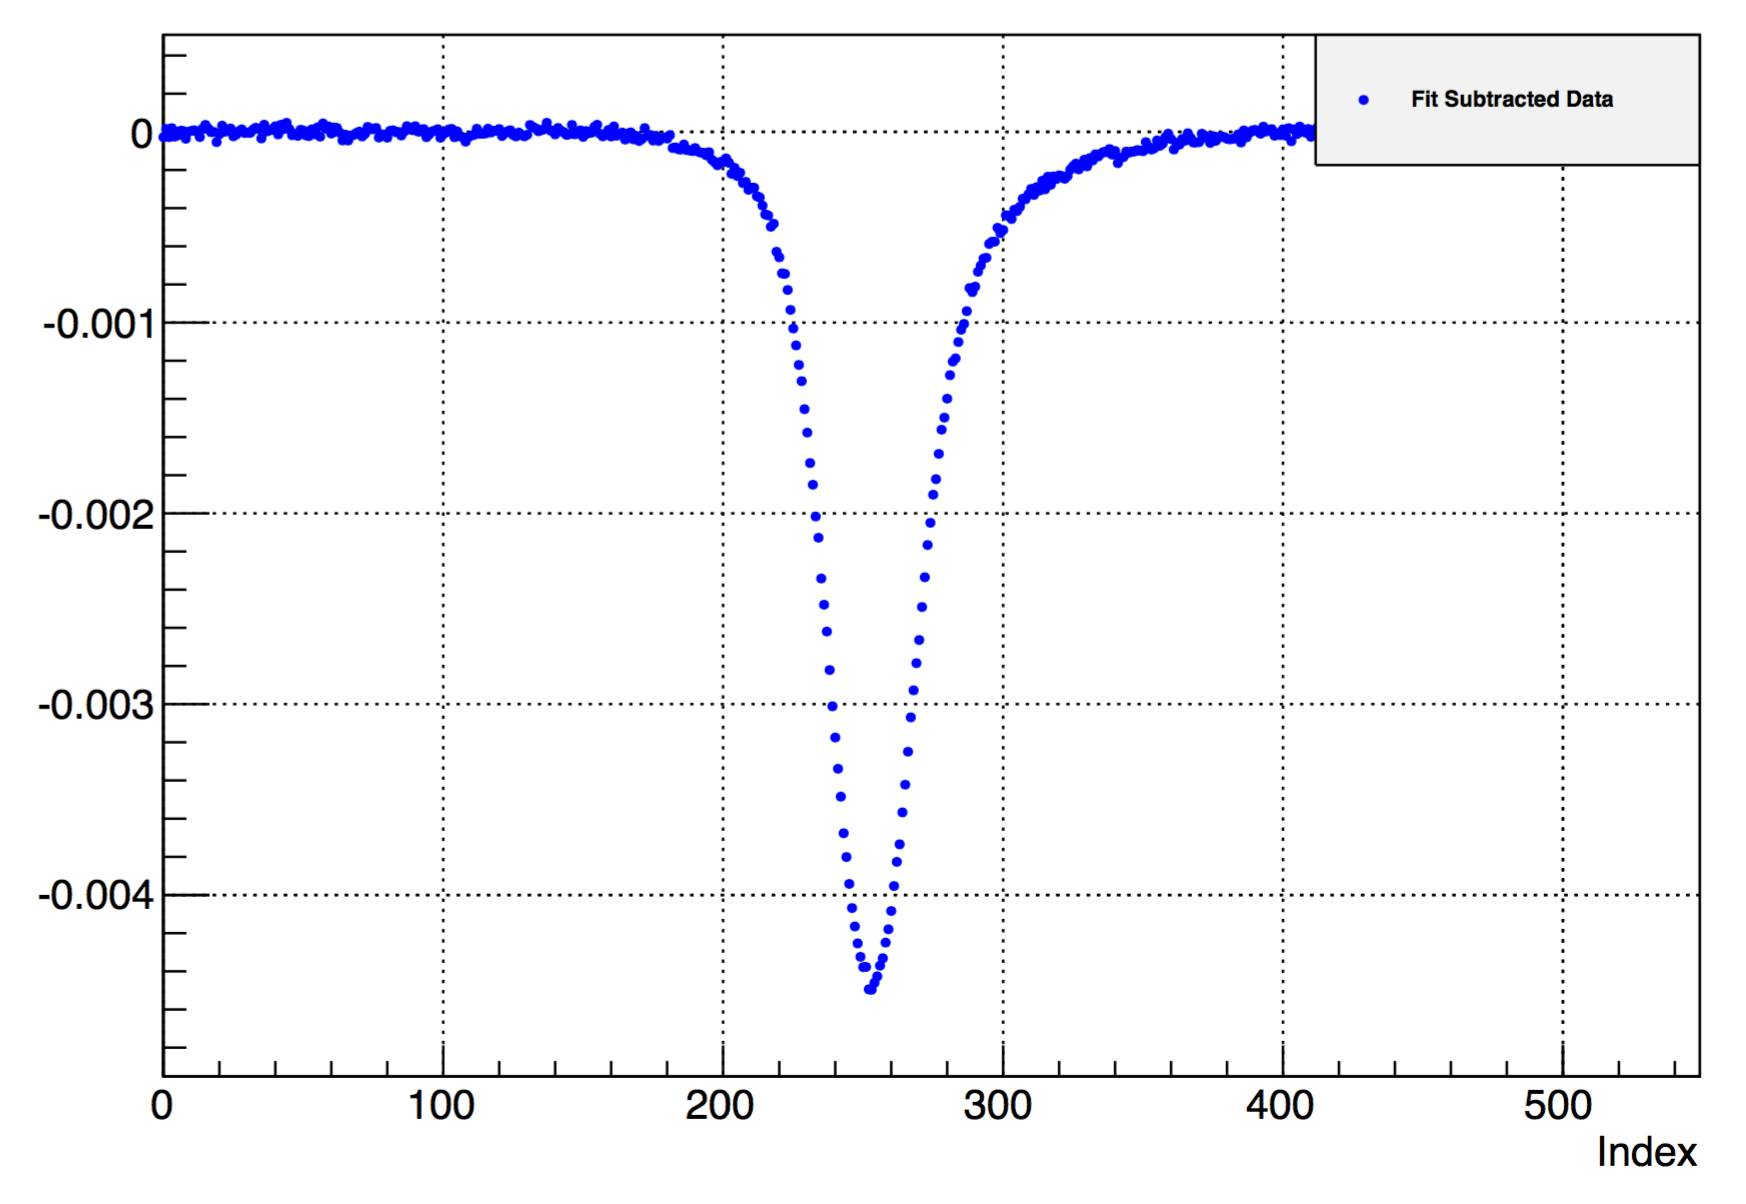
\includegraphics[width=\textwidth]{figs/target-NMR-signal.png}
    \caption{NMR signal after the subtraction. \label{C5S3SS3F1b}}
  \end{subfigure}
  \caption[Target NMR signals.]{An example of the target NMR signals. The $x$-axis index is proportional to the frequency of the RF generator. \label{C5S3SS3F1}}
\end{figure}

\begin{figure}[p!]
  \centering
  \begin{subfigure}[t]{0.9\textwidth}
    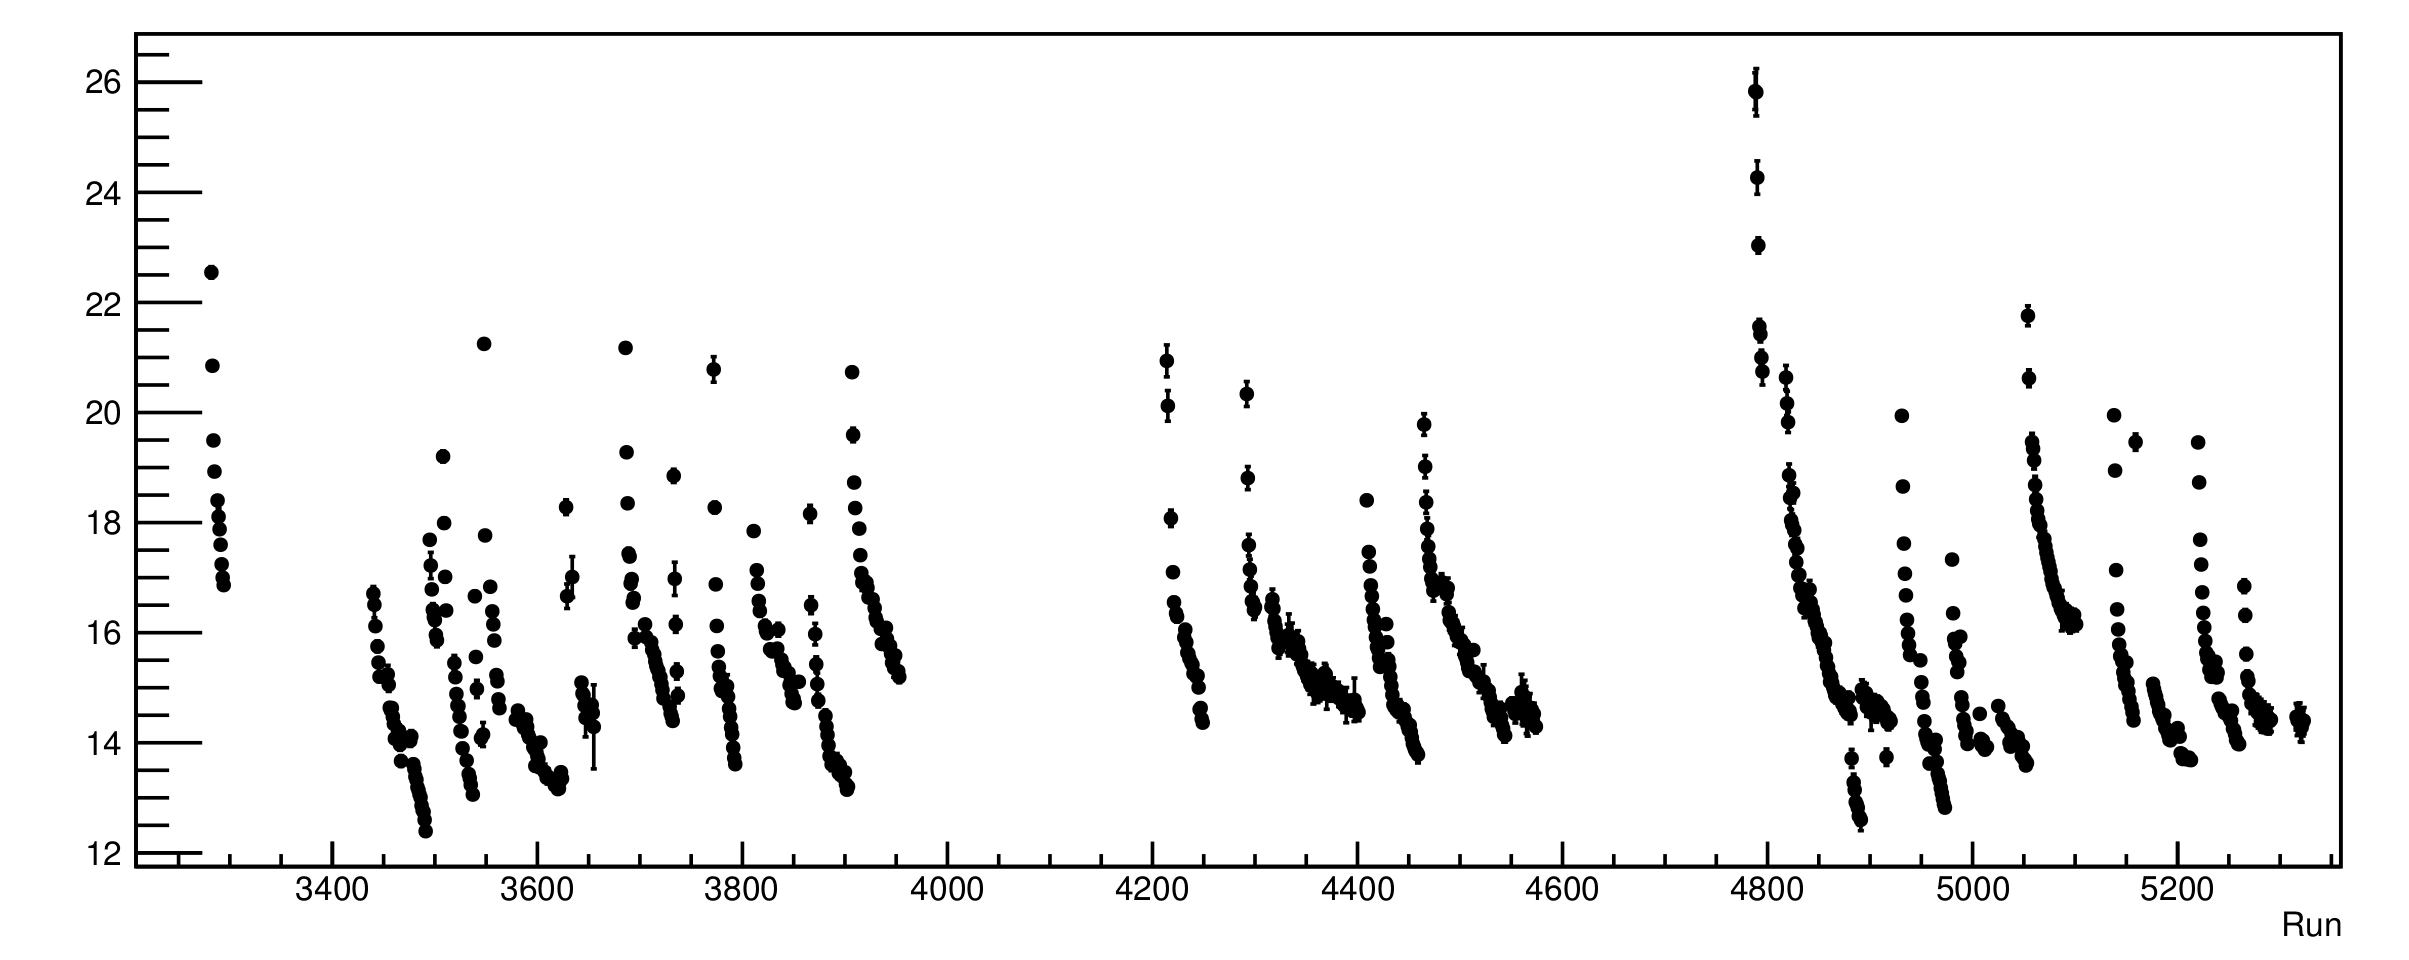
\includegraphics[width=\textwidth]{figs/target-polarization-25.png}
    \caption{2.5T target field configuration. \label{C5S3SS3F2a}}
  \end{subfigure}
  \begin{subfigure}[t]{0.9\textwidth}
    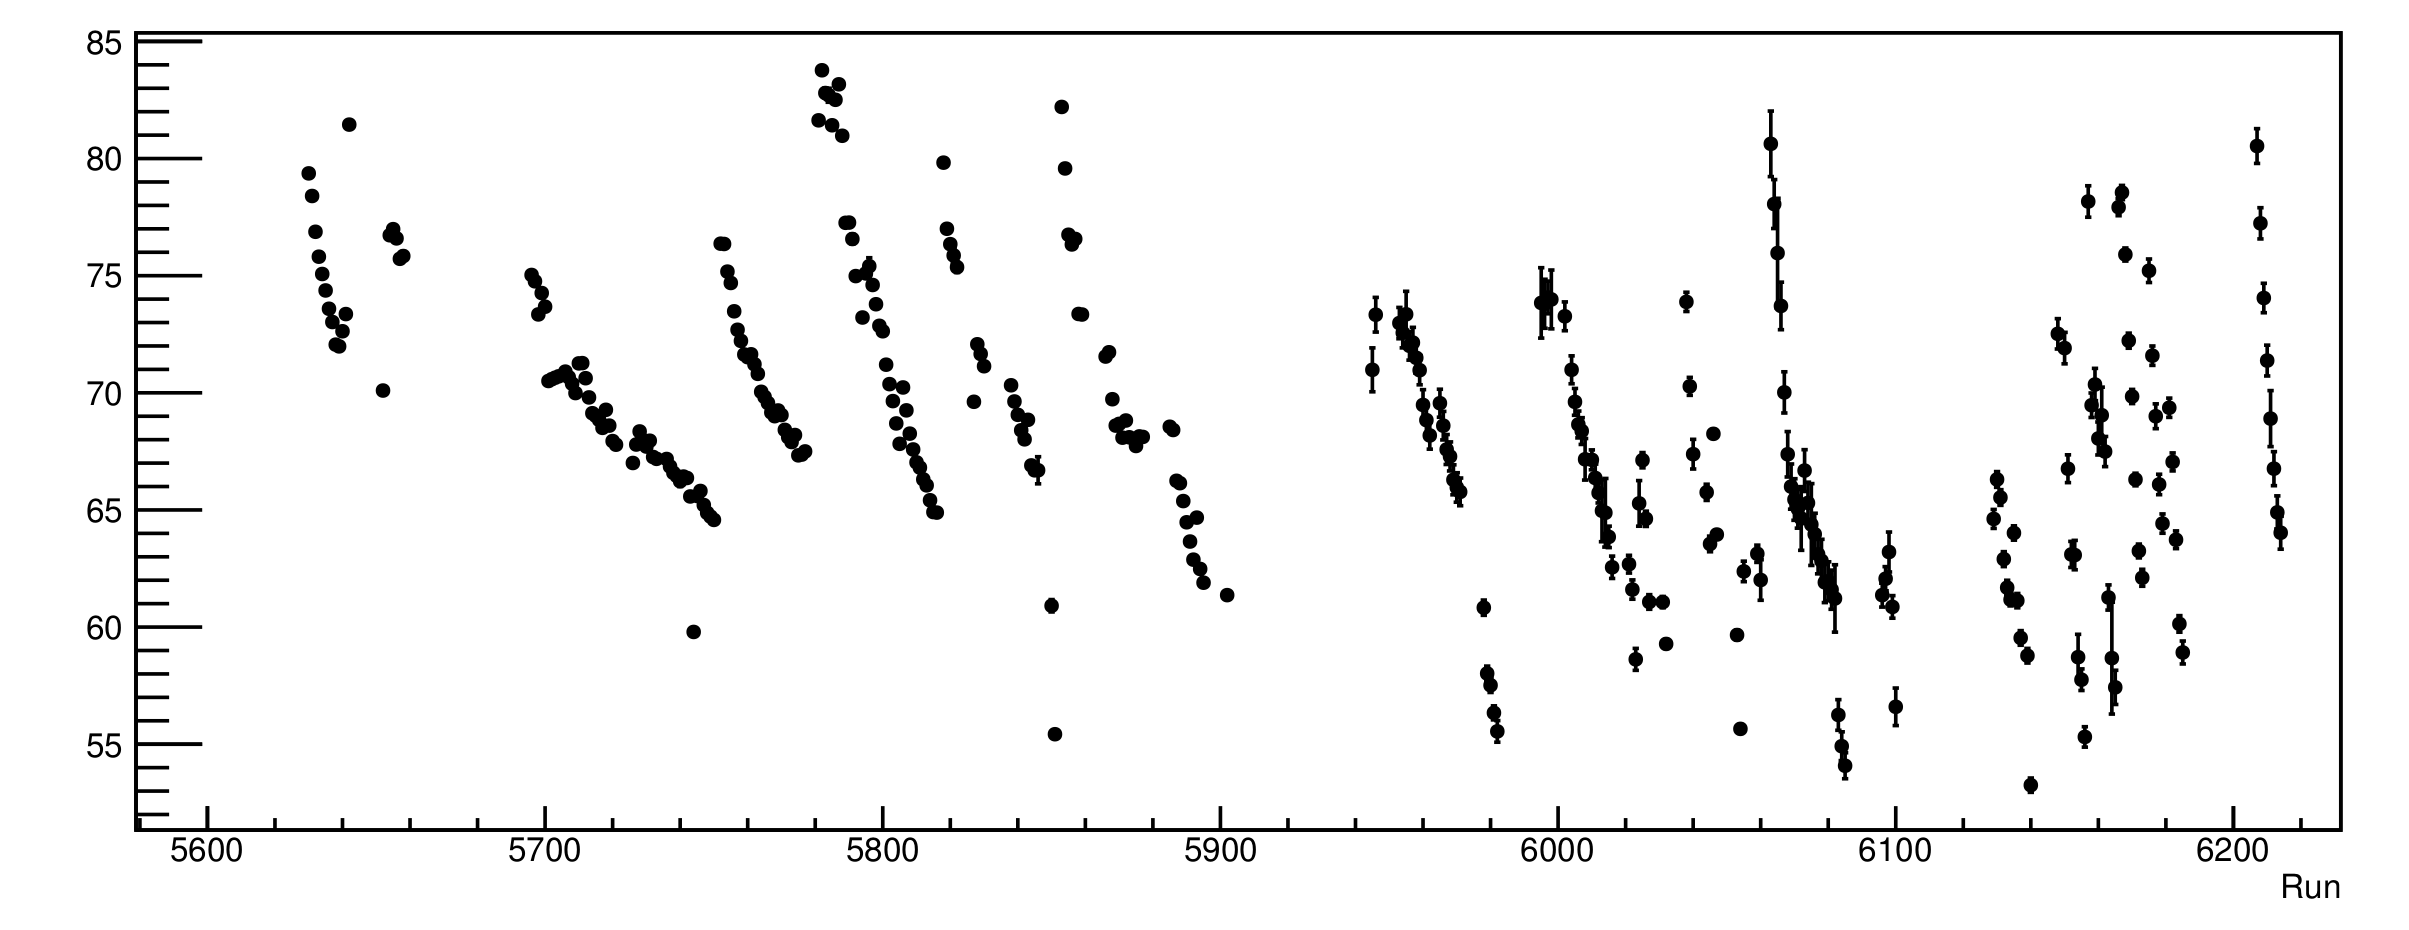
\includegraphics[width=\textwidth]{figs/target-polarization-50.png}
    \caption{5.0T target field configuration. \label{C5S3SS3F2b}}
  \end{subfigure}
  \caption[Target polarization results.]{Target polarization results during the experiment. Plot reproduced from \cite{Badman2013}. \label{C5S3SS3F2}}
\end{figure}

The output complex voltage $V(\omega,\chi)$ is proportional to the impedance of the circuit (\cref{C5S3SS3E2}). The NMR signal is composed with $V(\omega,\chi)$, together with the $Q$-meter response in the absence of $\chi$, $V(\omega,0)$, which is always referred as the ``$Q$-curve''. The $Q$-curve is measured by setting the target field so that the Larmor frequency is outside the range of the frequency scan of the $Q$-meter. The two signals are subtracted and the real part of the voltage is selected out by electronics, which gives the NMR signal $S(\omega)$:
\begin{equation} \label{C5S3SS3E3}
S(\omega) = \Re[V(\omega,\chi)-V(\omega,0)]\approx\chi''(\omega).
\end{equation}
Combining \cref{C5S3SS1E2,C5S3SS3E1,C5S3SS3E3}, the polarization $P$ can be expressed in terms of the thermal polarization $P_{\mathrm{TE}}$ and the ratio of the integral of two NMR signals $S_{\mathrm{TE}}$ and $S_{\mathrm{enh}}$, where $S_{\mathrm{TE}}$ is the NMR signal at thermal equilibrium and $S_{\mathrm{enh}}$ is the NMR signal under microwave irradiation (when the target is polarized):
\begin{equation} \label{C5S3SS3E4}
P = \frac{\int_0^\infty S_{\mathrm{enh}}(\omega)\dd{\omega}}{\int_0^\infty S_{\mathrm{TE}}(\omega)\dd{\omega}}P_{\mathrm{TE}}.
\end{equation}
\Cref{C5S3SS3F1} shows the raw voltage signal and the NMR signal.

The $S_{\mathrm{TE}}$ curve is measured several times during the experiment, which is referred to as the TE measurement. For each different NH${}_3$ sample, the numbers of the TE measurements varied from 1 to 8 measurements, depending on the time available. The polarization was then calculated via \cref{C5S3SS3E4} on a run-by-run basis. \Cref{C5S3SS3F2} shows the final polarization results. An average polarization of 70\% and 15\% was seen for the 5.0 T and 2.5 T configurations of the target field respectively.

The uncertainty of the polarization measurement arises from two major reasons. One is the uncertainty of the NMR signal. The other one is the uncertainty in the magnetic field and temperature readings, which contribute to the $P_{\mathrm{TE}}$ polarization calculation. The target polarization uncertainty is still being finalized, but the current result is $\sim$1.2\% \cite{Badman2013}.

\section{Hall A High Resolution Spectrometers}
\label{C5S4}

E08-027 uses the standard Hall A high resolution spectrometers (HRS) to detect the scattered electrons \cite{Alcorn2004}. It contains a nearly identical pair of spectrometers, which are referred to as HRS-L (left arm) and HRS-R (right arm) respectively. The main characteristics of HRS are summarized in \Cref{C5S4T1}. Both arms of the HRS contain three quadrupoles and a dipole magnet in a QQDQ configuration as illustrated \Cref{C5S4F1}. The Q1, Q2 and Q3 are three superconducting quadrupoles to provide focusing: Q1 focuses in the vertical plane and Q2 and Q3 in the transverse plane. The momentum of the electrons that reach the detector package are determined by the superconducting dipole with a momentum resolution at the $10^{-4}$ level. The electrons are bent by the dipole magnet by an angle of \SI{45}{\degree}.

\begin{figure}[p!]
  \centering
  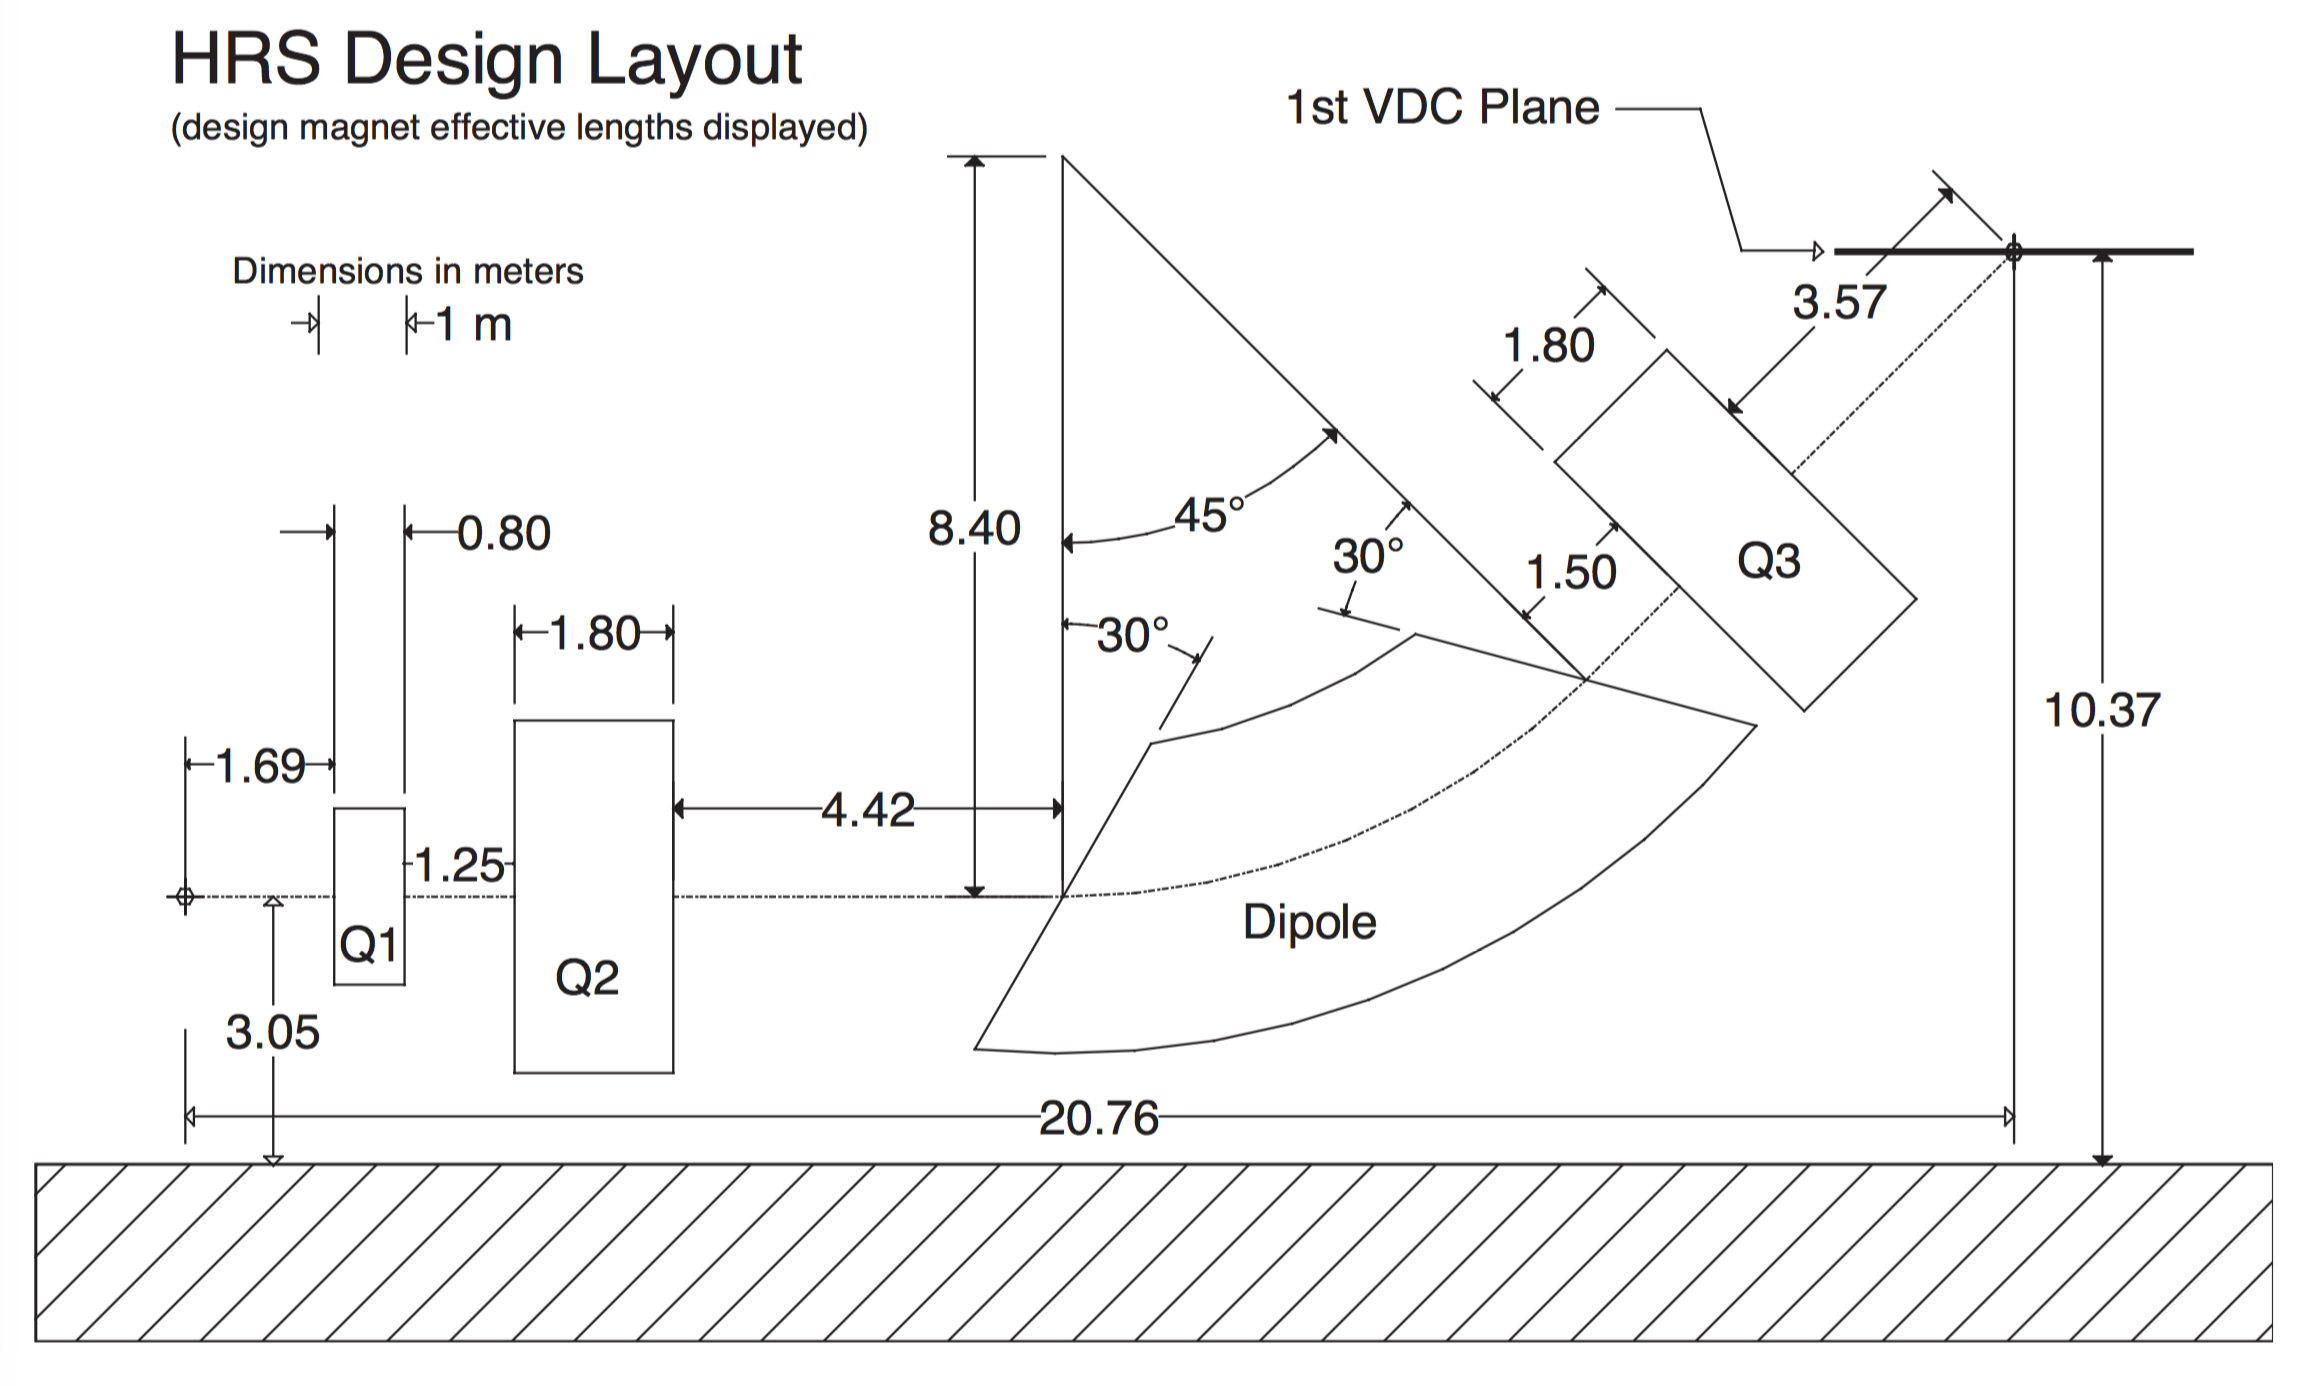
\includegraphics[width=\textwidth]{figs/HRS.png}
  \caption[Magnet configuration for HRS.]{Magnet configuration for HRS. Also shown is the location of the first VDC tracking detector. Figure reproduced from \cite{Alcorn2004}. \label{C5S4F1}}
\end{figure}

\begin{table}[p!]
  \centering
  \begin{tabular}{|l|c|}
    \hline\hline
    Bending angle & \SI{45}{\degree} \\ \hline
    Optical length & 23.4 m \\ \hline
    Momentum range & 0.3$\sim$4.0 GeV/c \\ \hline
    Momentum acceptance & $\pm$4.5\% \\ \hline
    Momentum resolution & $1\times10^{-4}$ \\ \hline
    Angular range (HRS-L) & \SI{12.5}{\degree}$\sim$\SI{150}{\degree} \\ \hline
    Angular range (HRS-R) & \SI{12.5}{\degree}$\sim$\SI{130}{\degree} \\ \hline
    Angular acceptance (horizontal) & $\pm$30 mrad \\ \hline
    Angular acceptance (vertical) & $\pm$60 mrad \\ \hline
    Angular resolution (horizontal) & 0.5 mrad \\ \hline
    Angular resolution (vertical) & 1.0 mrad \\ \hline
    Solid angle at $\delta=0$, $y_0=0$ & 6 msr \\ \hline
    Transverse length acceptance & $\pm$5 cm \\ \hline
    Transverse position resolution & 1 mm \\ \hline
  \end{tabular}
  \caption[The characteristics of the HRS.]{The characteristics of the standard Hall A spectrometers. Table reproduced from \cite{Alcorn2004}. \label{C5S4T1}}
\end{table}

\subsection{Septum Magnet}
\label{C5S4SS1}

The experiment E08-027 measured the scattered electrons at $\sim$\SI{5.77}{\degree}. However, the HRS have a minimum achievable angle of \SI{12.5}{\degree}, that is mainly because the Q1 magnet would hit the beam pipe if the spectrometer is moved to a smaller angle. During the experiment, a pair of septum magnet was used to allow both spectrometers to reach angles down to \SI{5.77}{\degree} \cite{G2P}. The septum magnet pair was located in front of the Q1 entrence of the HRS and horizontally bent the electrons with scattering angle $\sim$\SI{5.77}{\degree} into the spectrometer located at \SI{12.5}{\degree}. The coils of the septum magnet burned twice during the experiment, which led to three different septum configurations. The detailed configurations are discussed in \Cref{C6S3SS1}.

\subsection{Detector Package}
\label{C5S4SS2}

\begin{figure}[b!]
  \centering
  \begin{subfigure}[t]{0.49\textwidth}
    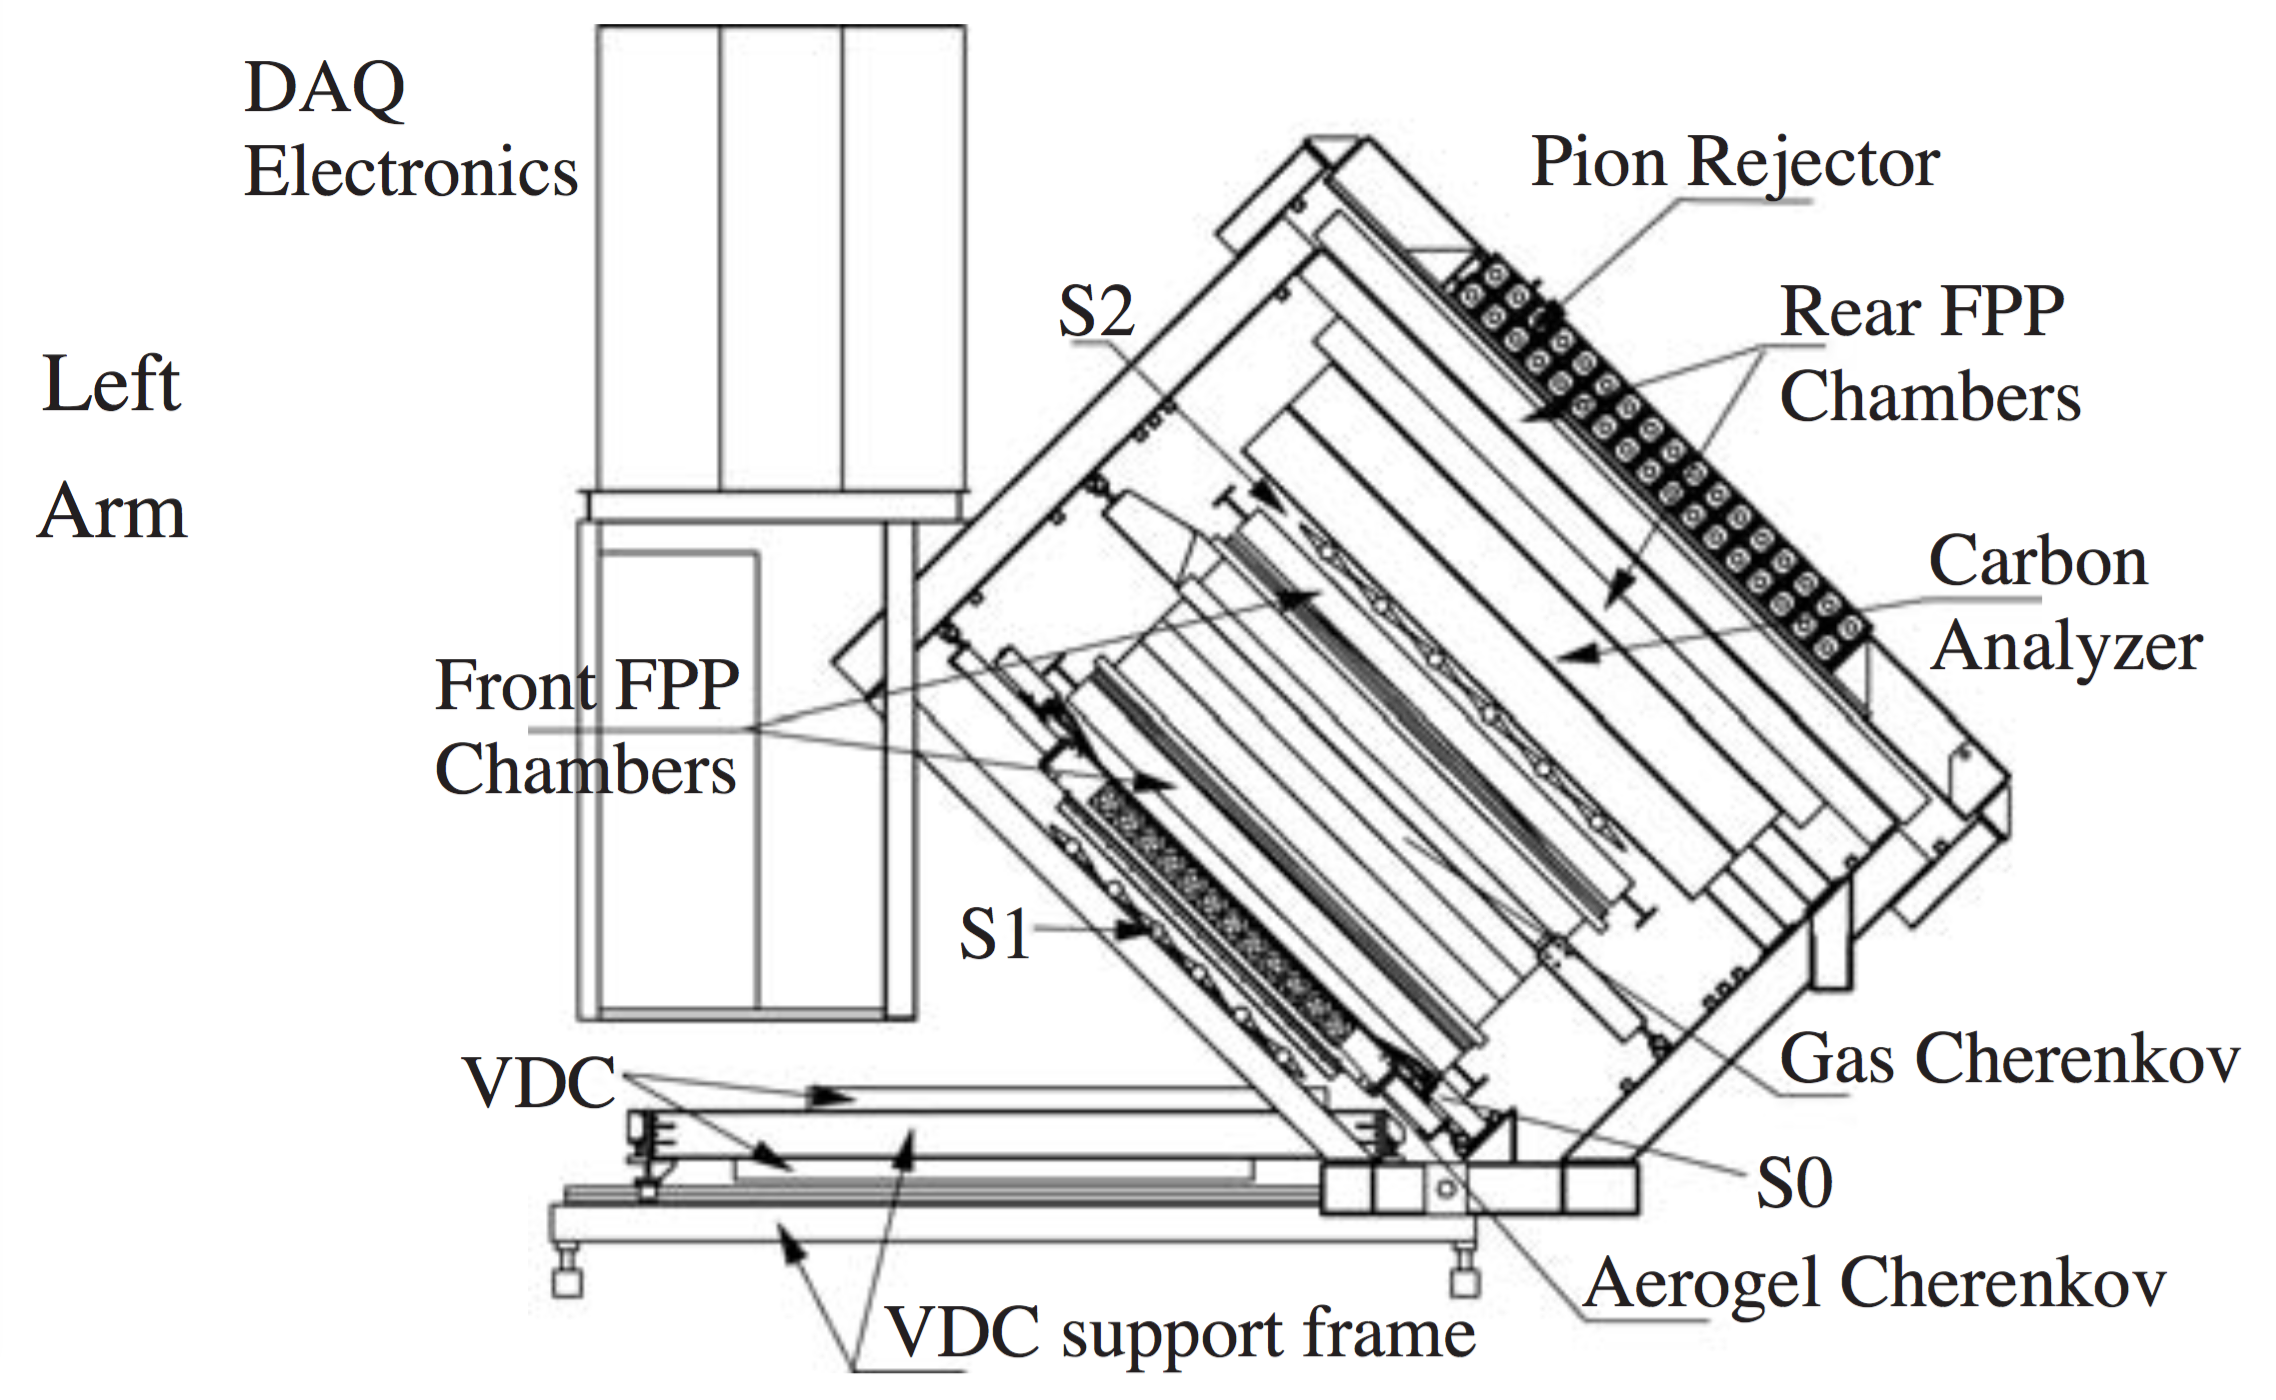
\includegraphics[width=\textwidth]{figs/detector-package-left.png}
    \caption{Left arm. \label{C5S4SS2F1a}}
  \end{subfigure}
  \begin{subfigure}[t]{0.49\textwidth}
    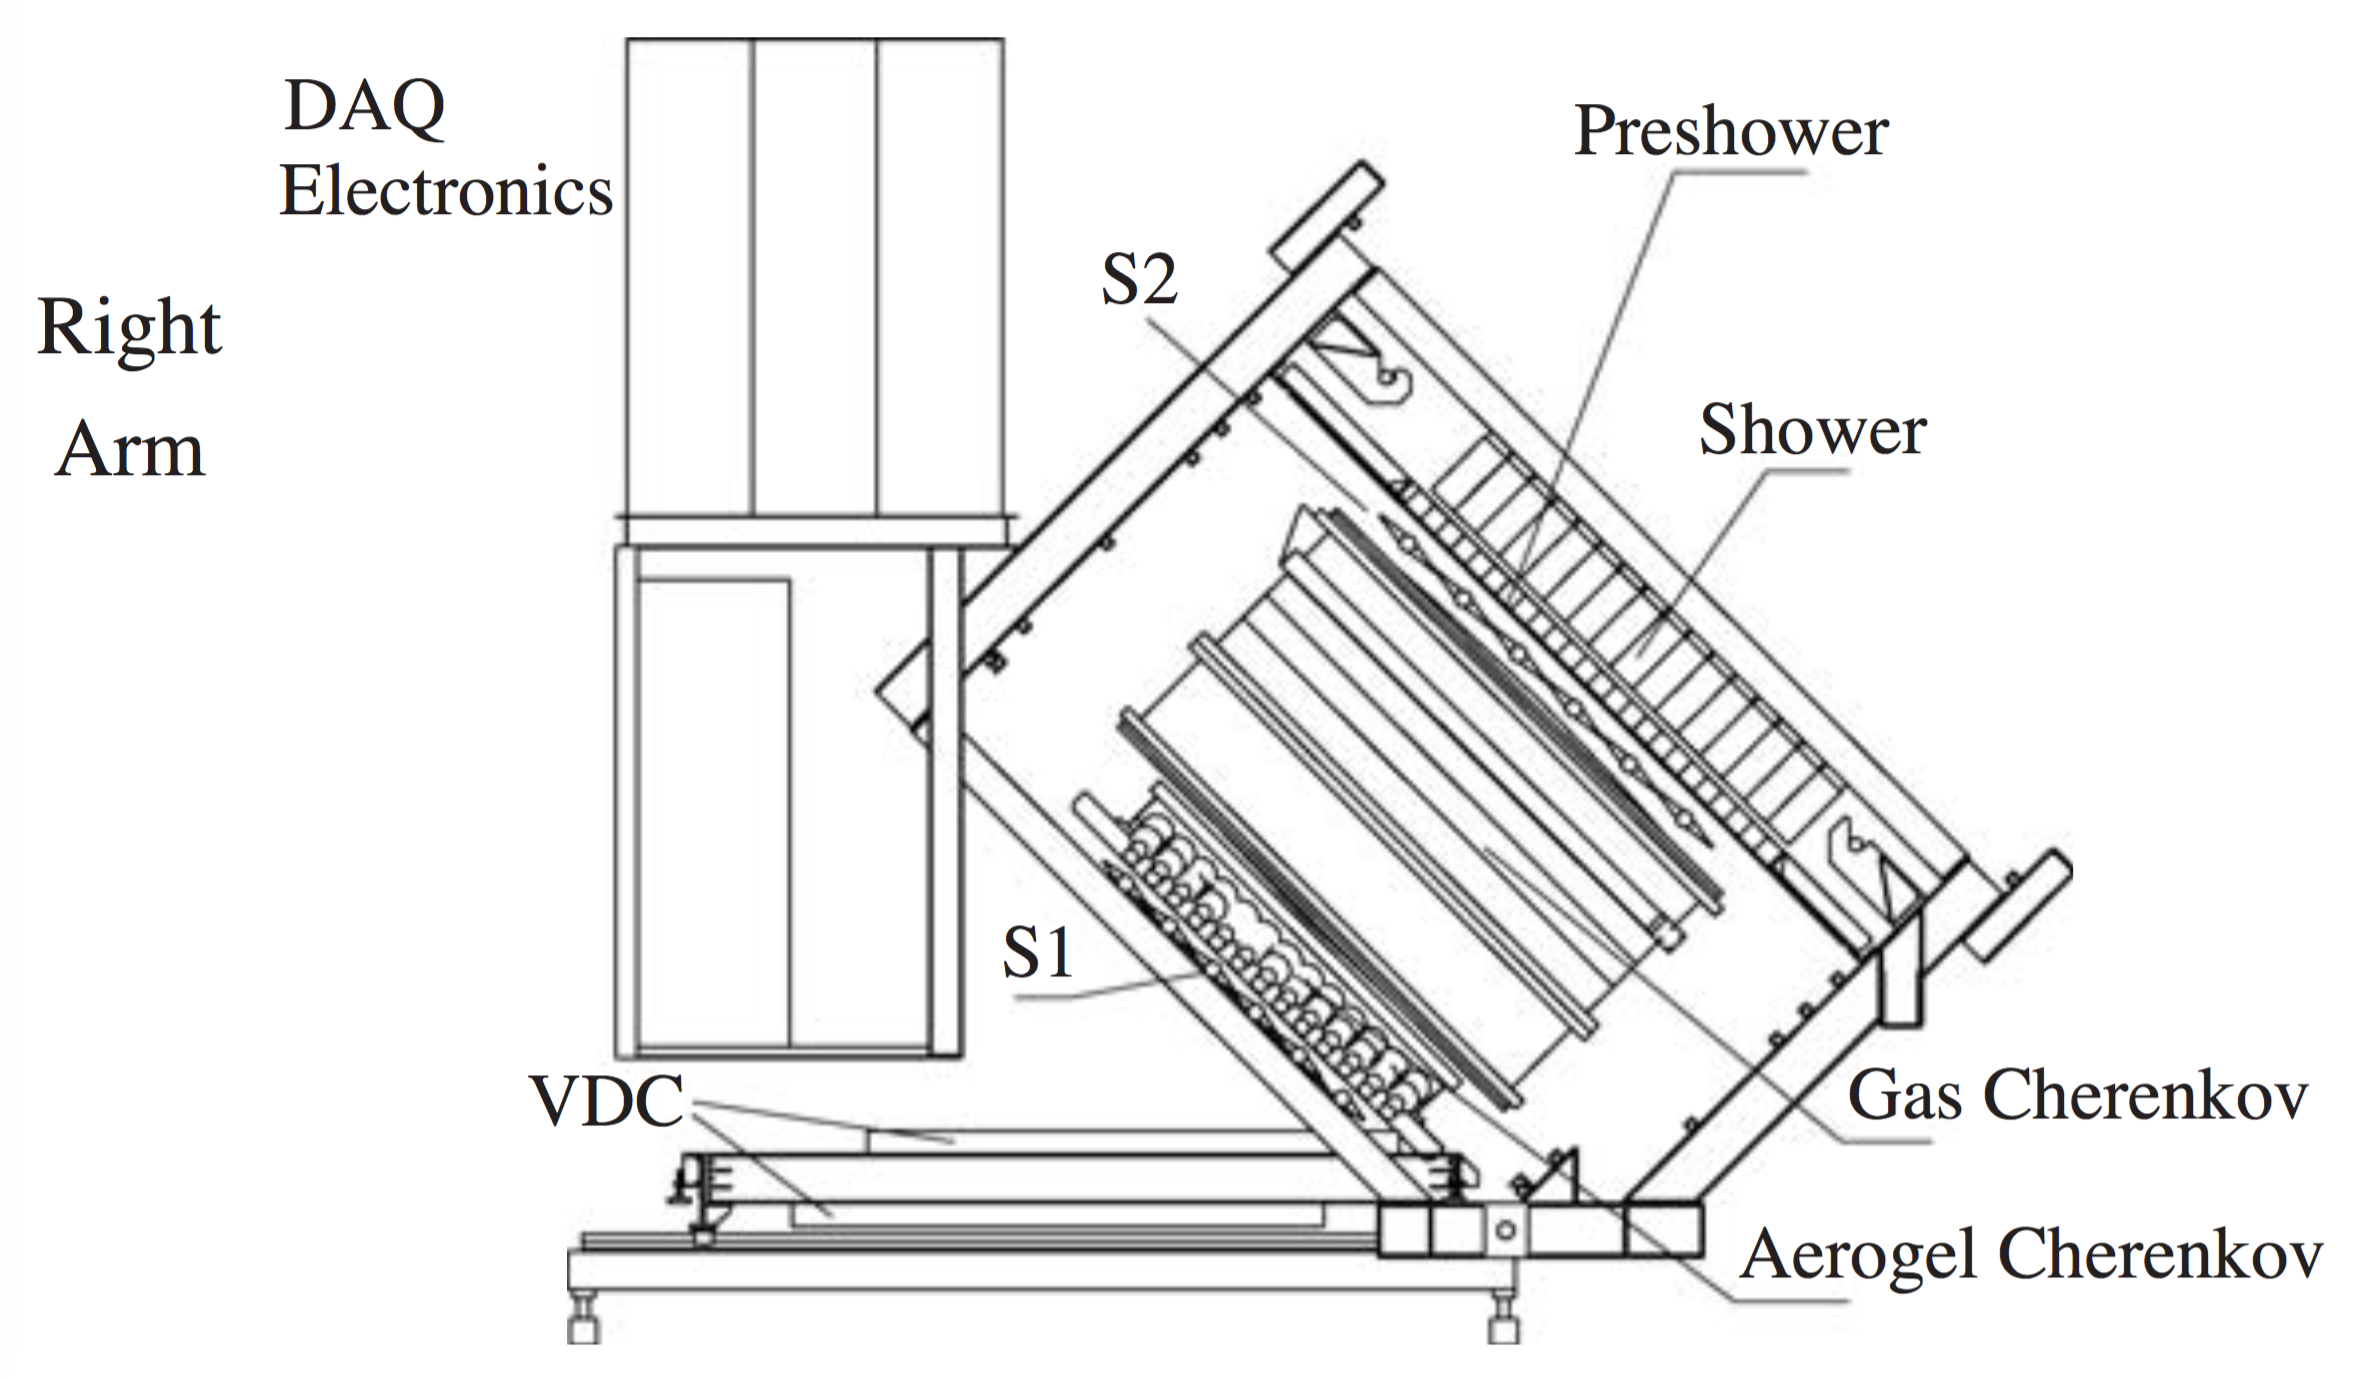
\includegraphics[width=\textwidth]{figs/detector-package-right.png}
    \caption{Right arm. \label{C5S4SS2F1b}}
  \end{subfigure}
  \caption[Detector package of HRS.]{Detector package of HRS. Note that only the VDC, scintillators (S1 and S2), gas Cherenkov detector and the calorimeters (pion rejectors in HRS-L, shower and pre-shower in HRS-R) were used during E08-027. Figure reproduced from \cite{Alcorn2004}. \label{C5S4SS2F1}}
\end{figure}

The detector package of the HRS is installed in a shielding hut together with the DAQ electronics at the end of the magnet group. The standard layout of the detector package is shown in \Cref{C5S4SS2F1}. The trajectory and the momentum of the scattered particle is determined by a pair of vertical drift chambers. Then the particles pass through a pair of plastic scintillator planes which generate the trigger for DAQ system. A gas Cherenkov detector and a set of lead glass calorimeters (pion rejectors in HRS-L, shower and pre-shower in HRS-R) are used for particle identification (PID). The main difference between two arms is the second layer of the calorimeters. The lead-glass blocks are aligned perpendicular to the particle trajectories in the left arm, whereas in the right arm the blocks in the second layer are oriented parallel to the trajectories.

\subsubsection{Vertical Drift Chambers}

The vertical drift chambers (VDC) package in each spectrometer consists of two VDC chambers, each composed of two wire planes in a UV configuration \cite{Fissum2001} as shown in \Cref{C5S4SS2F2}. The U and V planes are orthogonal and lie in the laboratory horizontal plane. They are inclined at an angle of \SI{45}{\degree} with respect to the dispersive direction of the dipole. Each plane contains 368 sense wires, spaced 4.24 mm apart. The upper and lower VDC chambers are separated by about 335 mm. The spectrometer focal plane is referred as the first wire plane that the particles traverse through. The concept of focal plane is important to the spectrometer optics study which will be discussed in details in \Cref{C6}.

\begin{figure}[tb!]
  \centering
  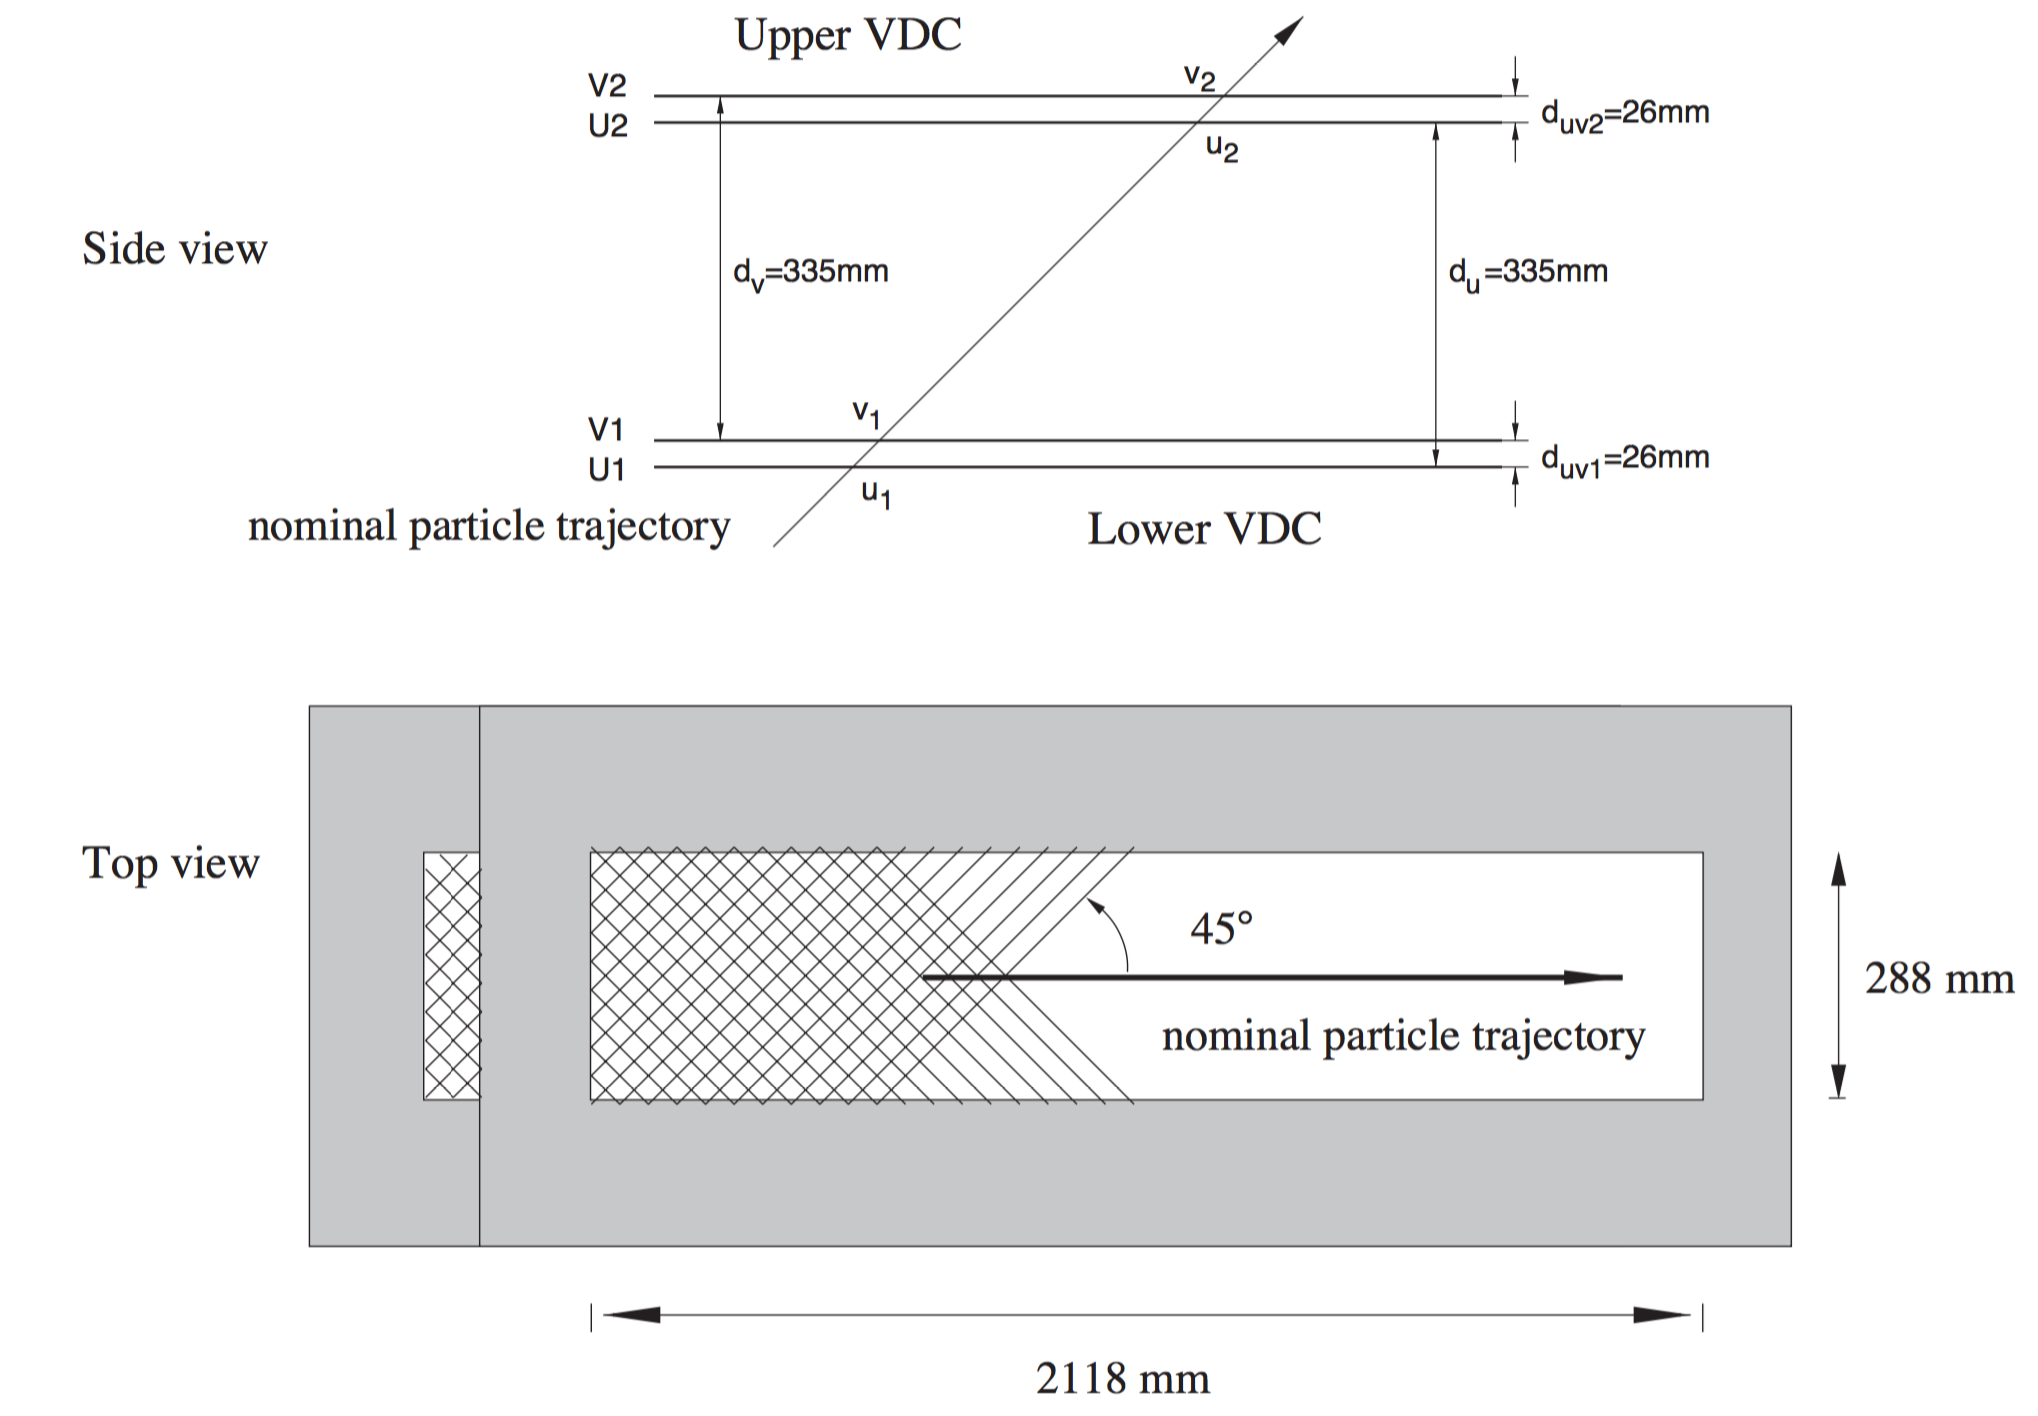
\includegraphics[width=0.75\textwidth]{figs/VDC.png}
  \caption[Schematic diagram of the Hall A vertical drift chambers.]{Schematic diagram of the Hall A vertical drift chambers. Plot reproduced from \cite{Alcorn2004}. \label{C5S4SS2F2}}
\end{figure}

The chambers are filled with a gas mixture of argon (62\%) and ethane (38\%). Argon provides the ionizing medium while ethane absorbs the photons produced from ionization. The electric field of the VDCs is shaped by gold-plated Mylar planes powered at -4 kV. Ionized electrons drift along the electric field lines and rapidly accelerate towards the wire when they are close to a wire, producing a shower of secondary ionizations. The approaching avalanche of electrons induces a signal on the wire.

By design, the electrons that travel across the VDCs with an angle of \SI{45}{\degree} will fire four to six wires per plane. This provides an accurate reconstruction of the particle's trajectory. The trajectories are reconstructed with the timing information provided by time-to-digital converters (TDCs) which are connected to the wires. The timing information can be used to determine the drift distance for each wire. The cross-over point is then determined via a linear fit of drift distances versus the wire position. The position and angular resolution of the focal plane are approximately 100 $\mu$m and 0.5 mrad, respectively.

\subsubsection{Scintillator Planes}

Two plastic scintillator planes (S1 and S2m) separated by 2 m are used to form the trigger for the DAQ system. Both planes are made up of overlapping paddles of plastic scintillators \cite{Alcorn2004}. The S1 plane has 6 paddles and the S2m plane consists of 12 paddles. Each paddle is monitored by a pair of photomultiplier tubes (PMTs), one at each end. The timing resolution for each plane is about 0.3 ns.

The main trigger (referred as T3 for HRS-L and T1 for HRS-R) is formed as:
\begin{itemize}[parsep=0pt]
\item The left and right PMTs both fire on a paddle in S1;
\item The left and right PMTs both fire on a paddle in S2m;
\item The S1 and S2m paddles both fire within a specified timing window.
\end{itemize}
A secondary trigger (referred as T4 and T2 for left and right arm, respectively) is used to monitor the scintillator efficiency. The efficiency trigger is exclusive to T1(or T3) trigger and formed by requiring either the S1 or the S2m scintillator plane to have fired as well as a signal from the gas Cherenkov detector. These represent possibly good events but one of the scintillator planes failed to detect.

The triggers are sent to the trigger supervisor (TS) to determine if the DAQ system should record the event or not. The DAQ cannot record every event if the event rate is high since the processing and output need some time. The fraction of events which the DAQ records is represented by a quantity called the livetime $LT$ or deadtime $DT=1-LT$. The processing deadtime can be decreased by scaling the incoming events with a prescale factor $ps$ at the TS which means that only 1 of every $ps$ events is sent to the DAQ system. The livetime depends on the event type and helicity state. It is determined by the number of triggers sent to the DAQ system $NT_{\mathrm{acc}}$ and the total number of generated triggers $NT$ which is recorded by scalers:
\begin{equation} \label{C5S4SS2E1}
LT^{\pm} = \frac{ps\cdot NT_{\mathrm{acc}}^{\pm}}{NT},
\end{equation}

\begin{figure}[tb!]
  \centering
  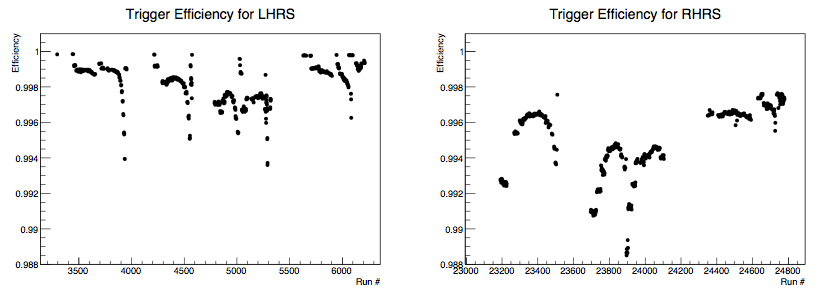
\includegraphics[width=\textwidth]{figs/trigger-efficiency.png}
  \caption[Trigger efficiencies of HRS.]{Trigger efficiencies of HRS. Plot reproduced from \cite{Zielinski2014a}. \label{C5S4SS2F3}}
\end{figure}

The trigger efficiency $\eta_{\mathrm{T}}$ is defined as:
\begin{equation} \label{C5S4SS2E2}
\eta_{\mathrm{T}} = \frac{NT_{\mathrm{main}}}{NT_{\mathrm{main}}+NT_{\mathrm{eff}}},
\end{equation}
where the $NT_{\mathrm{main}}$ are the total number of the T1 (or T3) trigger and $NT_{\mathrm{eff}}$ are the total number of the T2 (or T4) trigger described above. The deadtime effects of the triggers are corrected as follows:
\begin{equation} \label{C5S4SS2E3}
NT_{\mathrm{cor}} = \frac{ps\cdot NT}{LT},
\end{equation}
where $LT$ is calculated with \cref{C5S4SS2E1}. The trigger efficiency results are shown in \Cref{C5S4SS2F3}. Overall, the efficiencies are greater than 99.1\% \cite{Zielinski2014a}. Some substructure can be seen in the data, for example, the trigger efficiency at lower momenta tends to drop off. However, it is still safe to conclude that the correction to the cross-sections from the trigger efficiency is less than 1\%.

\subsubsection{Gas Cherenkov Detector}

The speed of light in a medium is always lower than the speed of light in vacuum. The ratio between two speeds is the index of refraction ($n$), which is a characteristic of the medium. Although the speed of light in the vacuum is the upper limit of the velocity of a particle, the velocity of a high energy particle may exceed the speed of light in a medium. A charged particle disrupts the local electromagnetic field when it travels through the medium. When the particle is traveling fast enough, the disturbance is left in the medium due to the limited response speed (speed of light in the medium), thus the energy contained in this disturbance radiates as a coherent shockwave, known as Cherenkov radiation \cite{Leo1994}. The wave is emitted in a cone. \Cref{C5S4SS2F4} shows the geometry of the Cherenkov radiation. The threshold for the production of Cherenkov radiation is given by:
\begin{equation} \label{C5S4SS2E4}
\beta c \geq\frac{c}{n},
\end{equation}
where $\beta=v/c$ is the velocity. The detection of the Cherenkov light is a very effective method to distinguish particles with different mass, especially when the momentum of the particle is measured independently.

\begin{figure}[tb!]
  \centering
  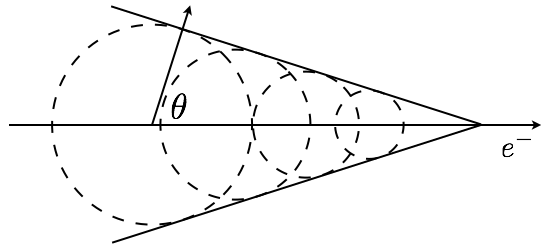
\includegraphics[width=0.5\textwidth]{figs/Cherenkov-radiation.png}
  \caption[Geometry of the Cherenkov radiation.]{Geometry of the Cherenkov radiation. The angle $\theta$ is given by $\cos\theta=1/n\beta$. \label{C5S4SS2F4}}
\end{figure}

In the detector package of HRS, a gas Cherenkov detector \cite{Iodice1998} is sandwiched between the two scintillator planes. The detector is filled with carbon dioxide gas with index of refraction $n=1.00041$. Since the speed threshold to produce Cherenkov radiation is $\beta\geq1/n$, the momentum threshold is therefore dependent on the mass of the particle:
\begin{equation} \label{C5S4SS2E5}
p_{\mathrm{thr}} = m_0\gamma v = m_0\frac{c}{\sqrt{n^2-1}}.
\end{equation}
In this case, the momentum threshold for electrons is 0.018 GeV, whereas the threshold for pions is 4.87 GeV. Thus, the Cherenkov detector can be used to identify the electrons and pions.

The detector has a path length of 1.5 m. Ten spherical mirrors is installed to focus the Cherenkov light onto 10 PMTs. The signals from the PMTs are sent to ADCs and are summed together, representing the total radiation produced by that particle. However, pions can cause a sizable background when they interact with materials in the detector. These background events are removed with the aid of a lead-glass calorimeter.

\subsubsection{Electromagnetic Calorimeter}

When a high energy particle traverses through a dense material, an electromagnetic cascade of photons and electron-positron pairs is generated \cite{Leo1994}. The light produced by the cascade is linearly proportional to the energy deposited in the material and can be detected by PMTs.

The calorimeters of the left and right arm of HRS are slightly different in construction \cite{Alcorn2004}. The HRS-L calorimeter is composed of two layers of the lead-glass blocks, each made of thirty-four blocks, oriented perpendicular to the particle trajectory. The blocks in the first layer are 14.5 cm$\times$14.5 cm$\times$30 cm while the blocks in the second layer are 14.5 cm$\times$14.5 cm$\times$35 cm. On HRS-R, the first layer of the calorimeter contains 48 10 cm$\times$10 cm$\times$35 cm lead-glass blocks which are oriented perpendicular to the particle trajectory, whereas the second layer is composed of 80 14.5 cm$\times$14.5 cm$\times$35 cm blocks which are oriented parallel to the particle trajectory. \Cref{C5S4SS2F5} shows the configurations of the calorimeters for both left arm and right arm. The major difference between the HRS-L and HRS-R calorimeters is that the HRS-R calorimeter is a total energy absorber, which means the scattered electrons will deposit all of their energies in the calorimeter since it is thick enough, while the HRS-L calorimeter is not a full energy absorber.

\begin{figure}[tb!]
  \centering
  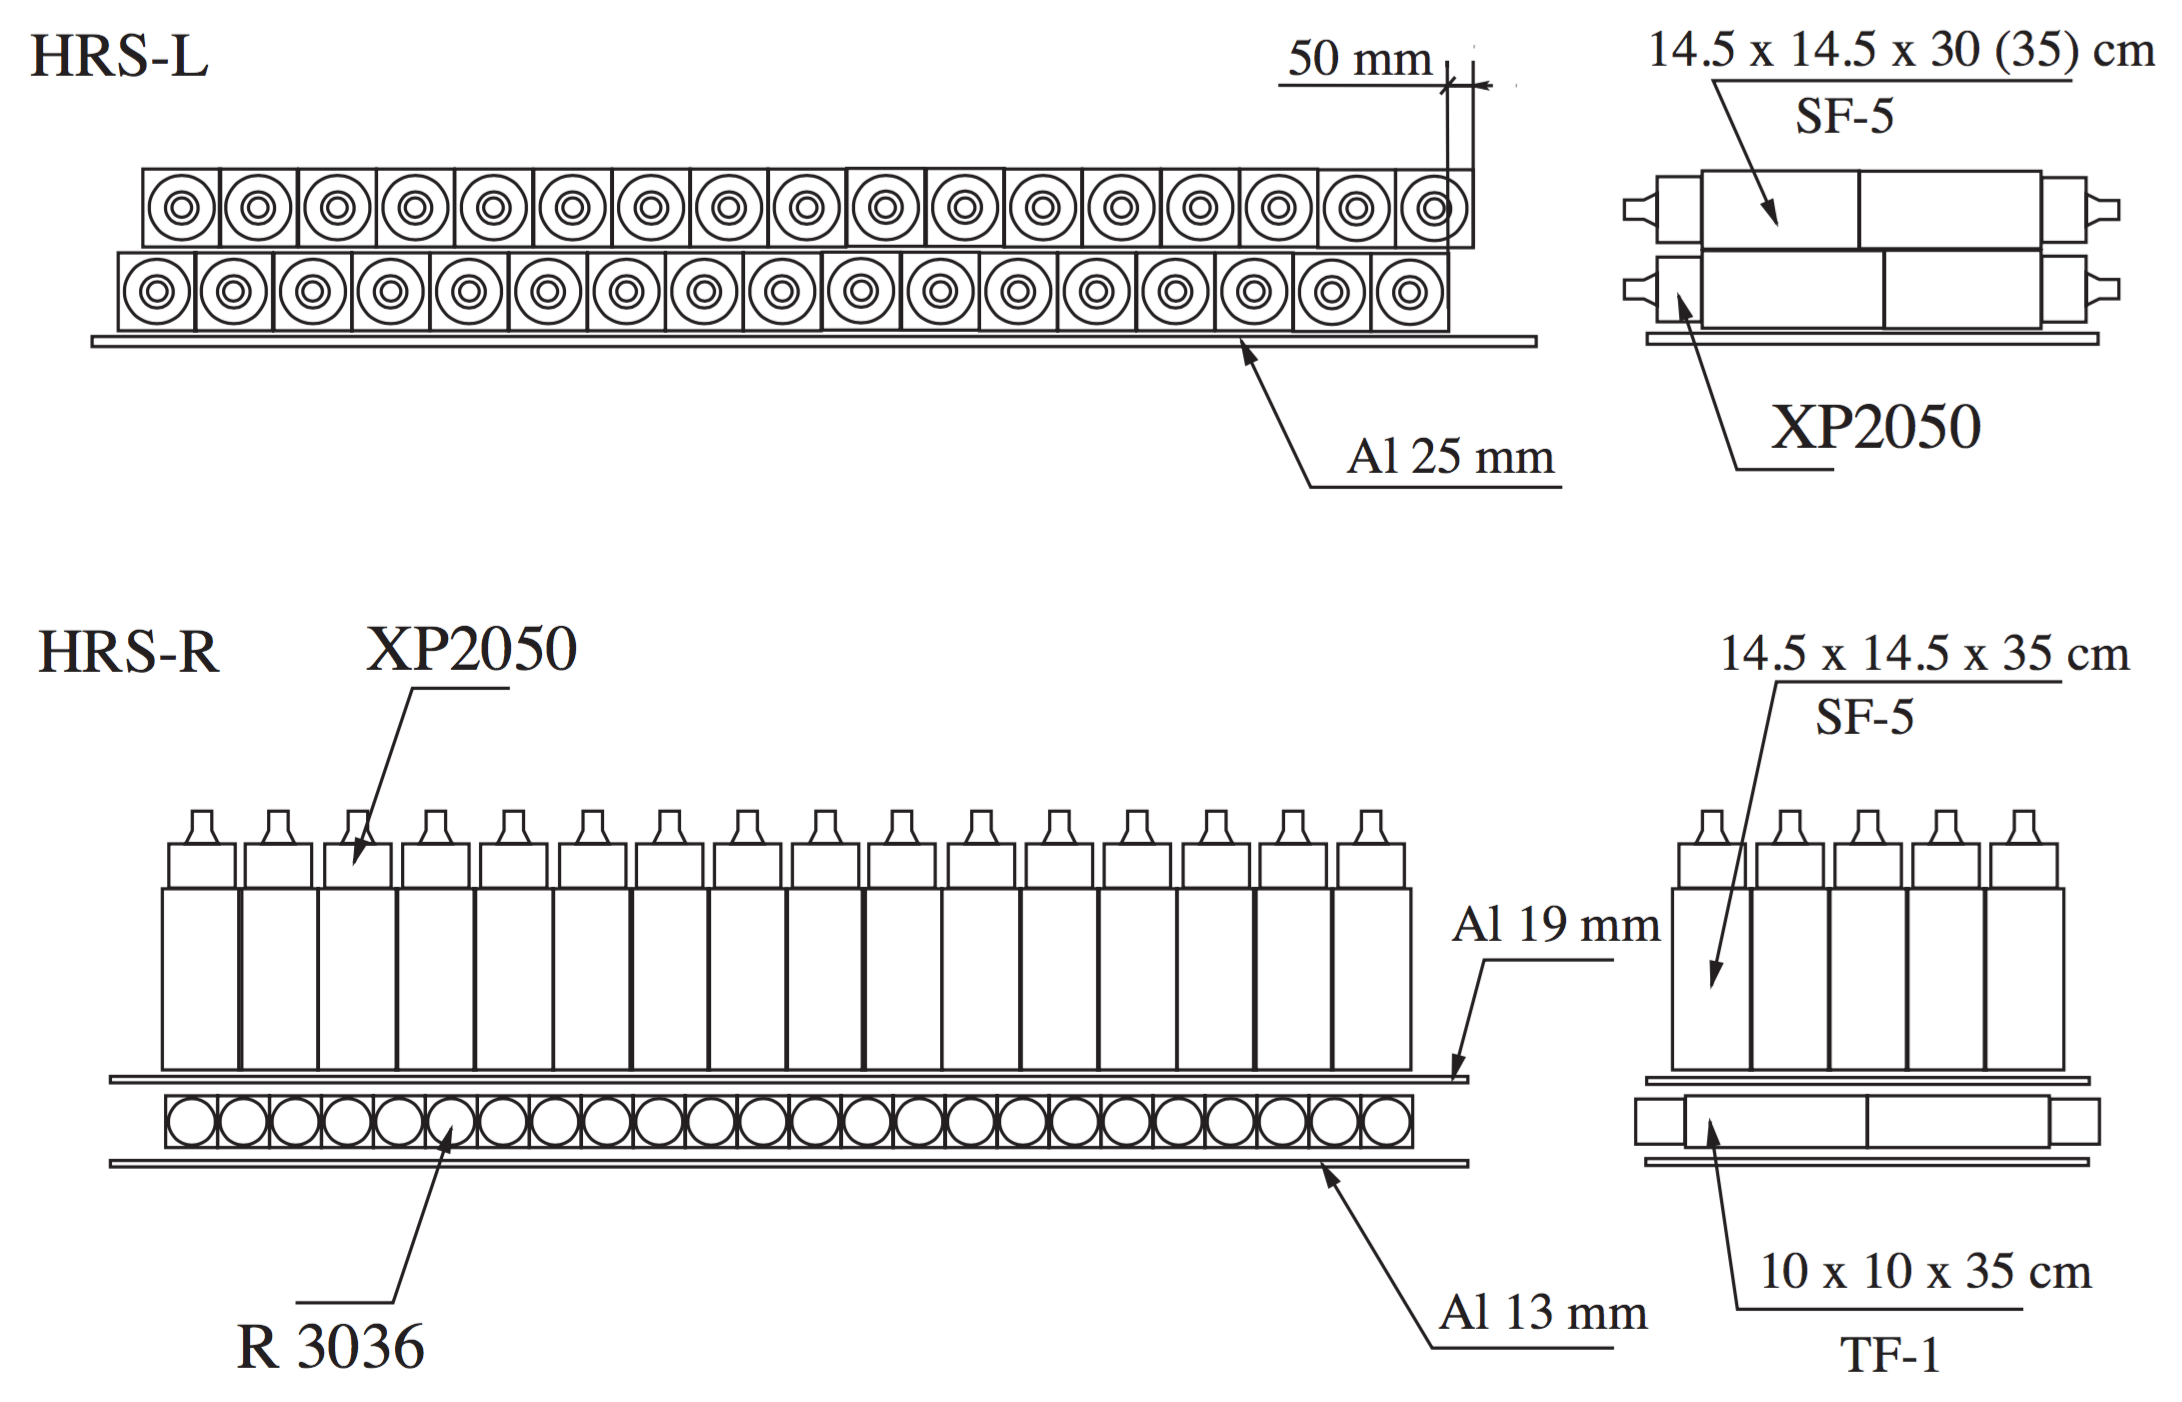
\includegraphics[width=0.8\textwidth]{figs/calorimeters.png}
  \caption[The electromagnetic calorimeters in the HRS.]{The electromagnetic calorimeters in the HRS. Plot reproduced from \cite{Alcorn2004}. \label{C5S4SS2F5}}
\end{figure}

%%%%%%%%%%%%%%%%%%%%%%%%%%%%%%%%%%%%%%%%%%%%%%%%%%%%%%%%%%%%%%%%%%%%%%
% -*-latex-*-

% -*-latex-*-

\chapter{Spectrometer Optics Study}
\label{C6}

In \Cref{C5}, we have introduced the experimental setup of E08-027. The strong transverse target field and the septum field makes the reconstruction of the kinematics of the scattered electrons, i.e., the spectrometer optics study, to be a challenge.

In the usual optics study procedure, the HRS is considered as an identical pair of magnetic spectrometers, each of which contains three quadrupoles and a dipole magnet in a QQDQ configuration as mentioned in the previous chapter. An optics matrix is introduced to represent the effect of the magnets configuration. Using this optics matrix, the kinematic variables of the scattered particles at the interaction point can be reconstructed from the signals recorded in the detectors. The optics matrix elements are determined through an established optics calibration procedure. They have been optimized over the full momentum ranges of both spectrometers and have been tested and shown to be stable.

During E08-027, a pair of septum magnets were used to bend the electrons with scattering angles $\approx$ \SI{5.77}{\degree} into the minimum spectrometer angle \SI{12.5}{\degree} of the HRS. The optics study for HRS with septum was first performed during E97-110 \cite{Sulkosky2005}. In E97-110, the optics matrix was re-optimized with the septum magnet added into the QQDQ magnets configuration. The basic optimization procedure was almost the same as the normal optics calibration procedure of the HRS. This procedure is preserved in E08-027, and thus the optics matrix method is used to describe the joint effect of the septum magnet and the HRS magnets.

In addition to the septa magnets, the optics calibration procedure needs to be modified to accommodate the effect from the strong transverse magnetic field of the polarized NH${}_3$ target. For E08-027, this was done by separating the motion of the scattered electron into two parts: the motion in the target field region, which can be calculated using the equation of motion of charged particles in the magnetic field, and the motion out of the target field region, which is described by the optics matrix. The optics study procedure and the corresponding reconstruction procedure were adjusted following this idea. In this chapter, we will summarize the procedure of the spectrometer optics study for E08-027.

\section{Coordinate Systems}
\label{C6S1}

In this section, an overview of the target and focal plane coordinate systems used in the spectrometer optics study is presented. More details can be found in Ref. \cite{Liyanage2002}. All coordinate systems are Cartesian unless otherwise stated. Note that in this section all references to angular coordinates should be considered as referring to the tangent of the angle.

\subsection[Hall Coordinate System]{Hall Coordinate System (HCS)}
\label{C6S1SS1}

The origin of the HCS is at the center of the Hall A, which is defined to be the intersection point of the beam and the vertical axis of the target. The $\hat{z}$ axis is along the beam line and points downstream, the $\hat{y}$ axis is vertically up, and the $\hat{x}$ axis is horizontal and pointing to the left if looking along $\hat{z}$ and upright along $\hat{y}$, see \Cref{C6S1SS1F1}.

\begin{figure}[p!]
  \centering
  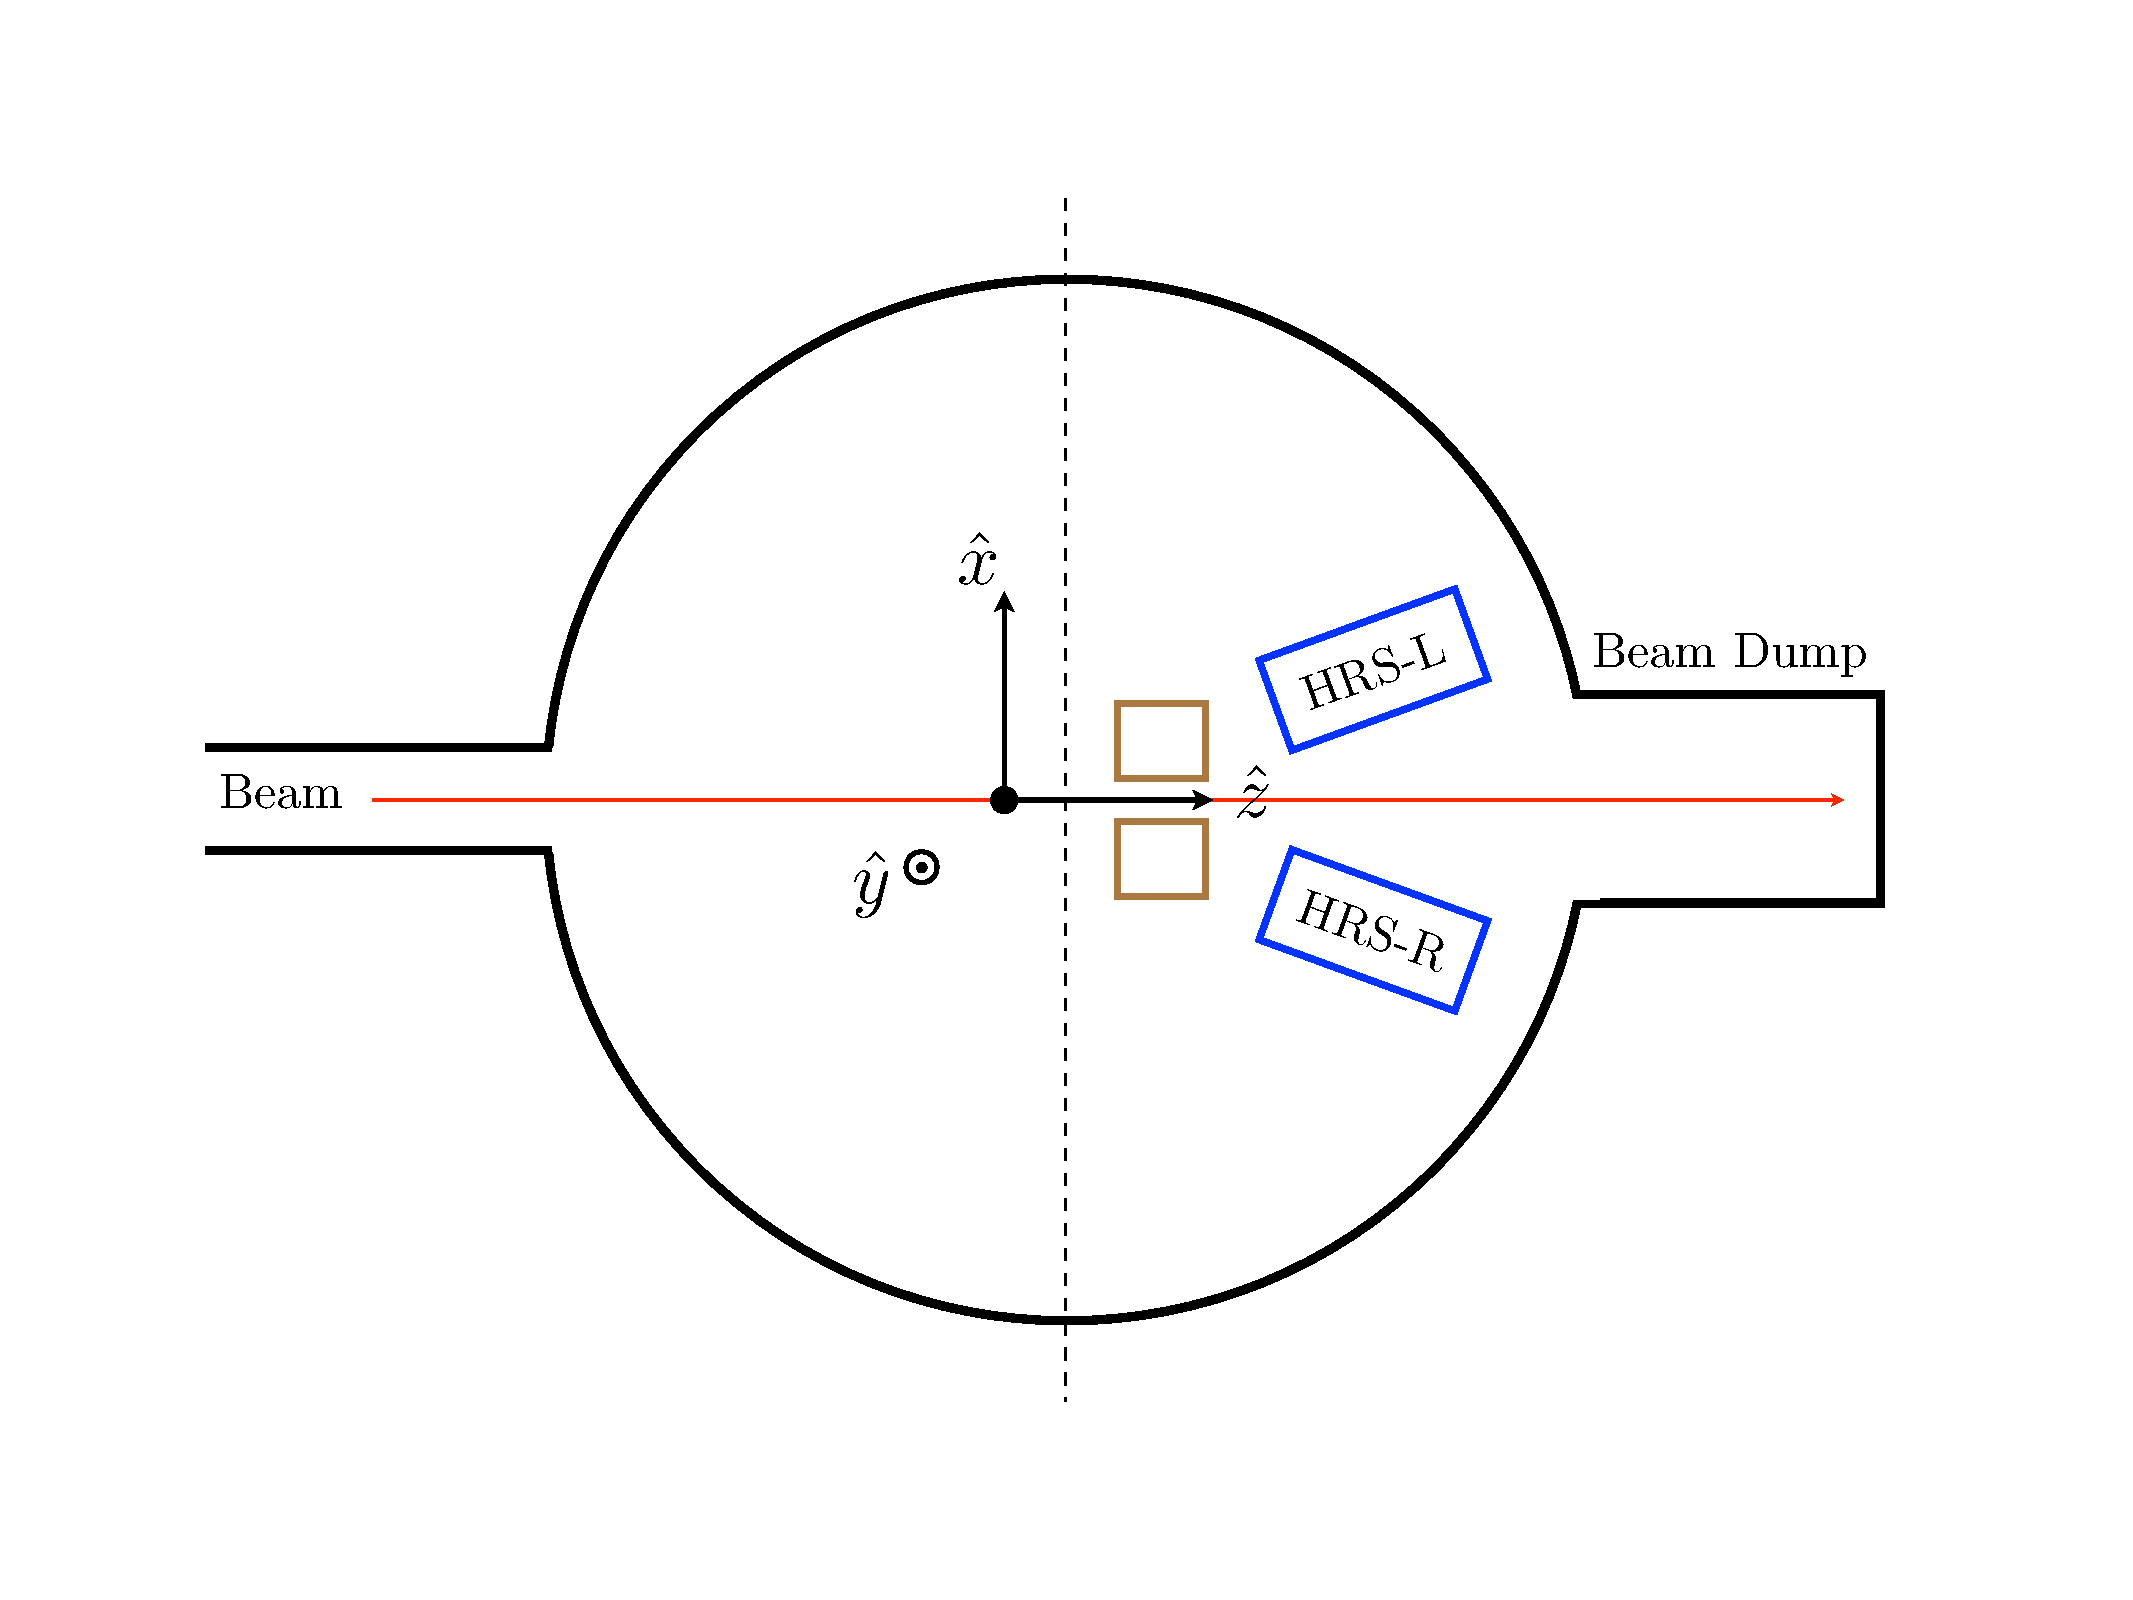
\includegraphics[width=0.75\textwidth]{figs/HCS.pdf}
  \caption[Hall coordinate system.]{Hall coordinate system (top view). \label{C6S1SS1F1}}
\end{figure}

\subsection[Target Coordinate System]{Target Coordinate System (TCS)}
\label{C6S1SS2}

\begin{figure}[p!]
  \centering
  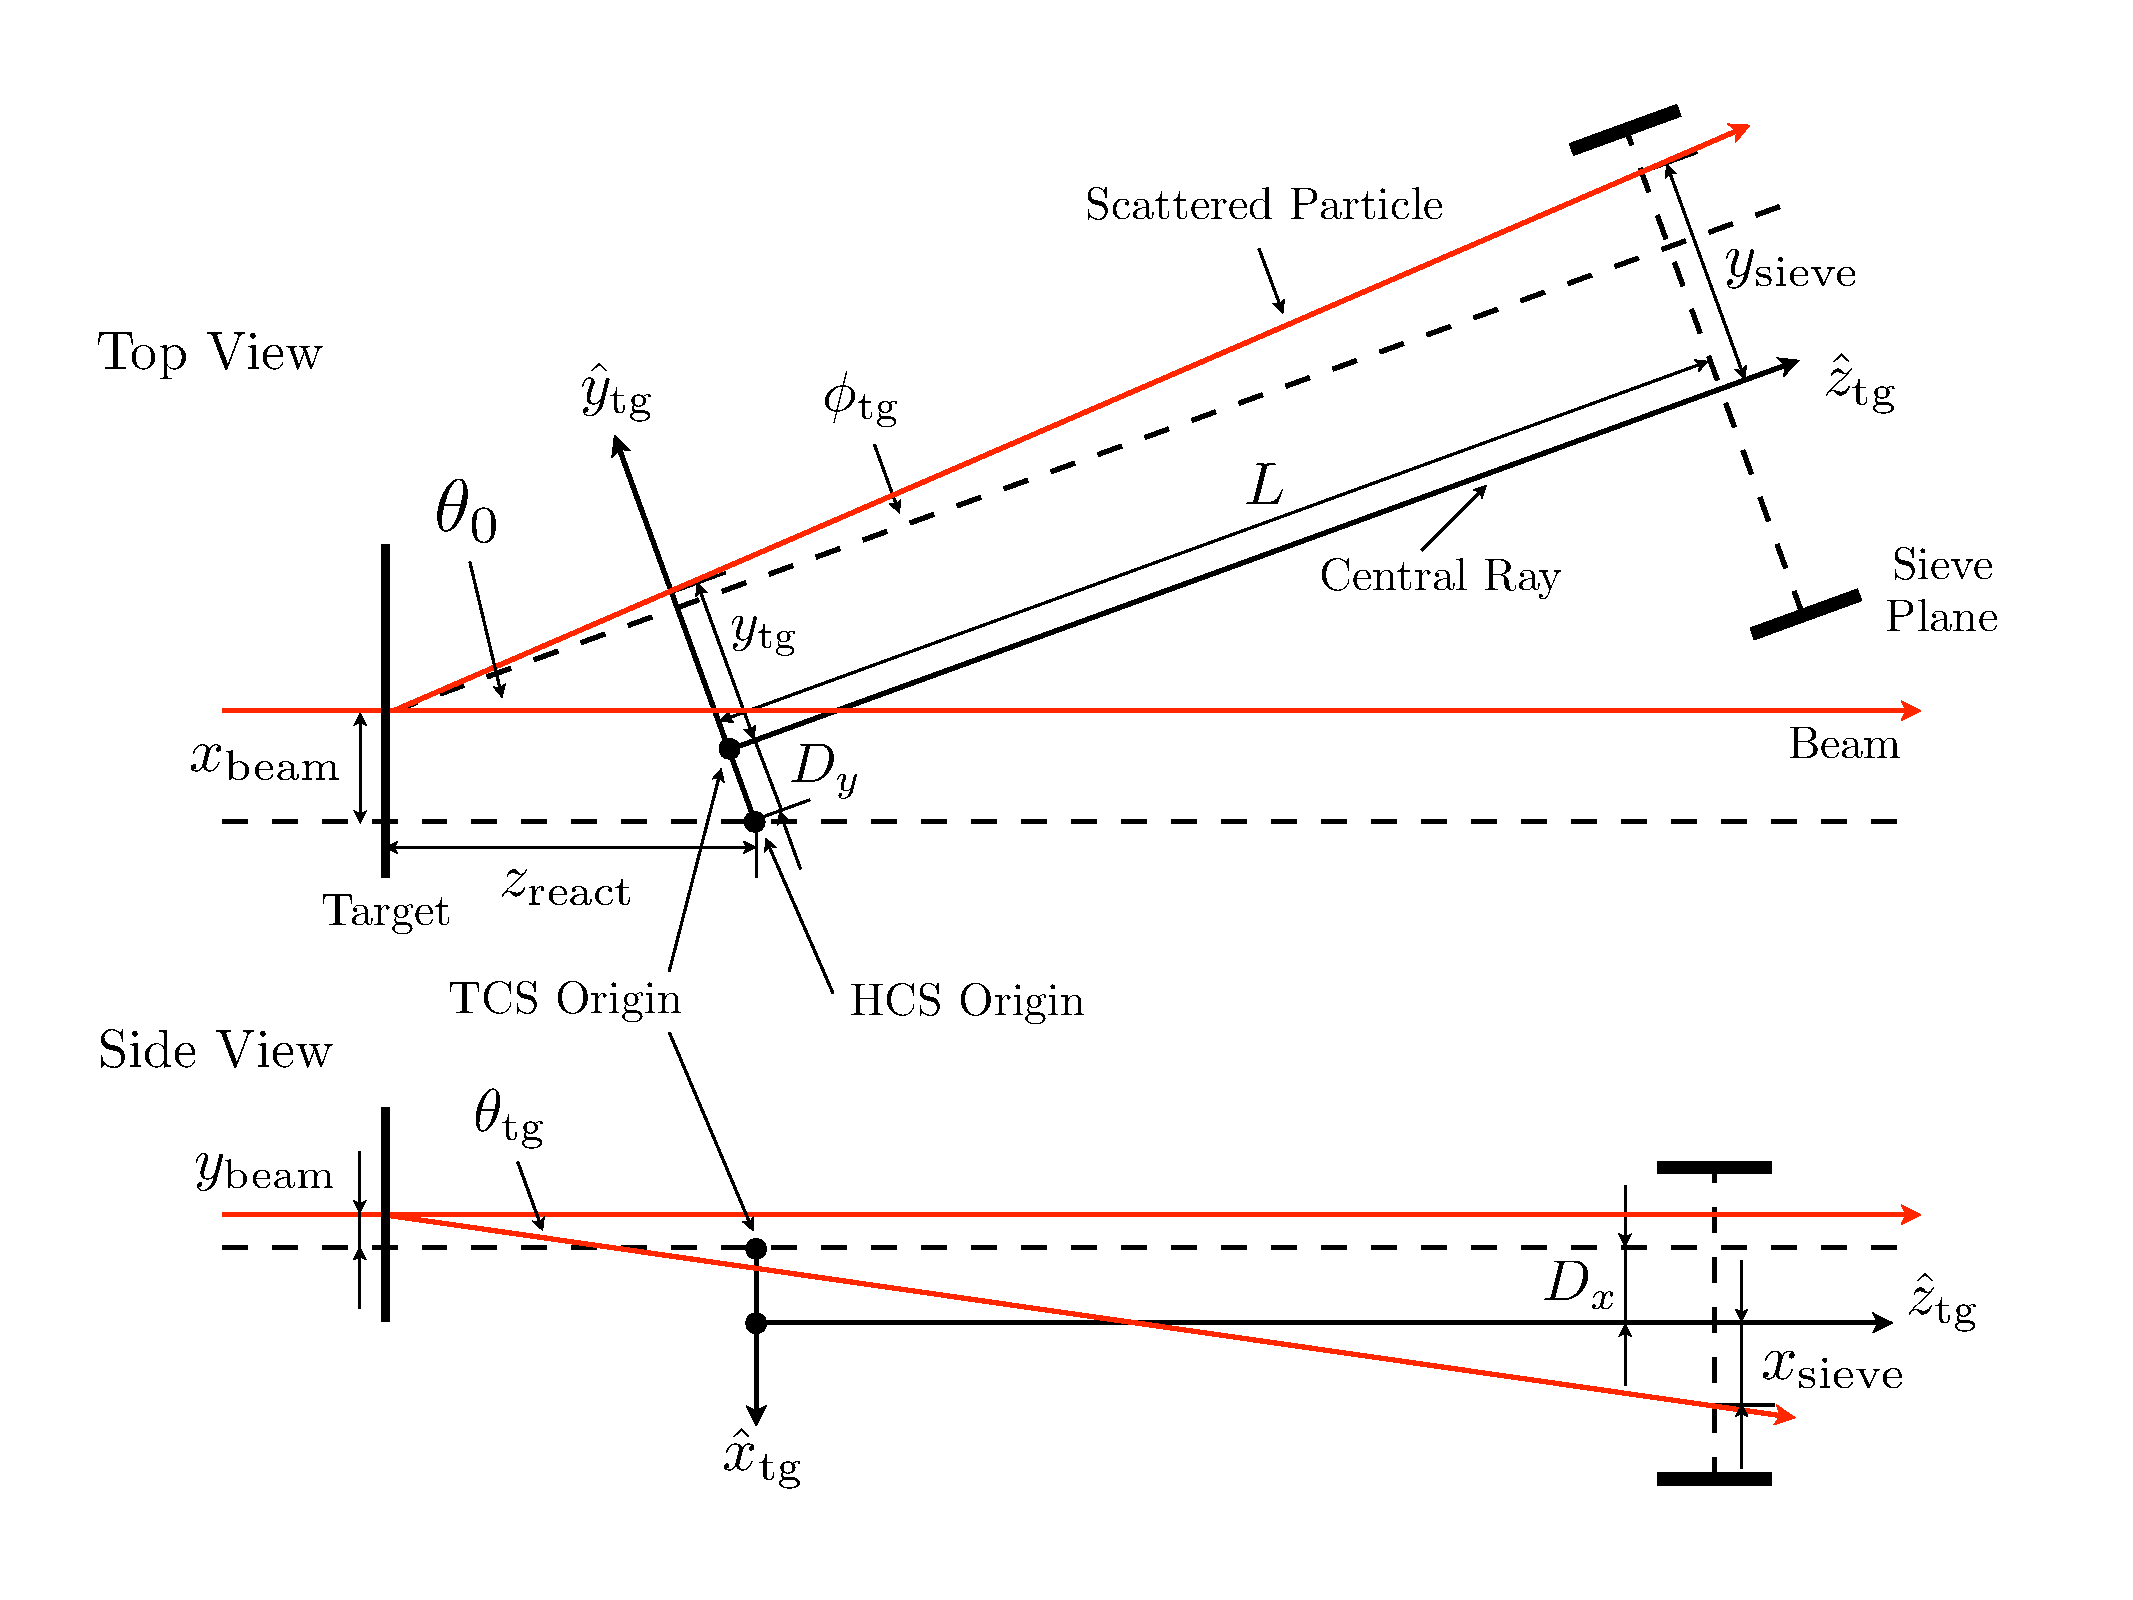
\includegraphics[width=0.9\textwidth]{figs/TCS.pdf}
  \caption[Target coordinate system.]{Target coordinate system (top and side views). $\theta_0$ is the spectrometer central angle, $L$ is the distance from the sieve slit to the TCS origin, $D_x$ and $D_y$ are the vertical and horizontal deviations of the spectrometer central ray to the HCS origin. \label{C6S1SS2F1}}
\end{figure}

Each of the two spectrometers has its own TCS. The $\hat{z}_{\mathrm{tg}}$ axis of the TCS is defined by the central ray of the sieve collimator for a given spectrometer which is the line perpendicular to the plane of the sieve slit passing through the center point of the central sieve slit hole. The $\hat{z}_{\mathrm{tg}}$ points away from the target towards the spectrometer and $\hat{x}_{\mathrm{tg}}$ is vertically down. Thus $\hat{y}_{\mathrm{tg}}$ is pointing to the left if looking along the $\hat{z}_{\mathrm{tg}}$ direction. Ideally, the $\hat{z}_{\mathrm{tg}}$ axis should pass through the hall center if the spectrometer points directly to the hall center and the sieve slit is perfectly centered. In this ideal case, the origin of the TCS coincides with the origin of the HCS. However, the origin of the TCS typically deviates from the hall center. The deviation can be measured by surveying the spectrometer pointing. The angle between $\hat{z}_{\mathrm{tg}}$ of the TCS and the $\hat{z}$ of the HCS is defined as the central angle $\theta_0$ of the spectrometer.

The kinematics of each scattering event is expressed as four variables in the TCS: the out-of-plane angle $\optt{tg}$ and the in-plane $\optp{tg}$ angle with respect to the central ray are given by $\mathrm{d}x/\mathrm{d}z$ and $\mathrm{d}y/\mathrm{d}z$ in the TCS; $\opty{tg}$ is given by the $y$ coordinate of the intersection point of the scattered particles's trajectory and the $z_{\mathrm{tg}}=0$ plane. The fourth variable $\delta$ is related to the momentum of the scattered particle:
\begin{equation} \label{C6S1SS2E1}
\delta = \frac{P-P_0}{P_0},
\end{equation}
where $P$ is the measured momentum of a particle and $P_0$ is the central momentum setting of HRS and septum \cite{Liyanage2002}. The scattering angle of the scattered particle can be calculated from the TCS variables:
\begin{equation} \label{C6S1SS2E2}
\optt{scat} = \arccos\left(\frac{\cos(\theta_0)-\optp{tg}\sin(\theta_0)}{\sqrt{1+\theta_{\mathrm{tg}}^2+\phi_{\mathrm{tg}}^2}}\right),
\end{equation}
where $\theta_0$ is the spectrometer certral angle. A diagram of the TCS as well as its relations with the HCS for the left arm is shown in \Cref{C6S1SS2F1}.

\subsection[Detector Coordinate System]{Detector Coordinate System (DCS)}
\label{C6S1SS3}

\begin{figure}[tb!]
  \centering
  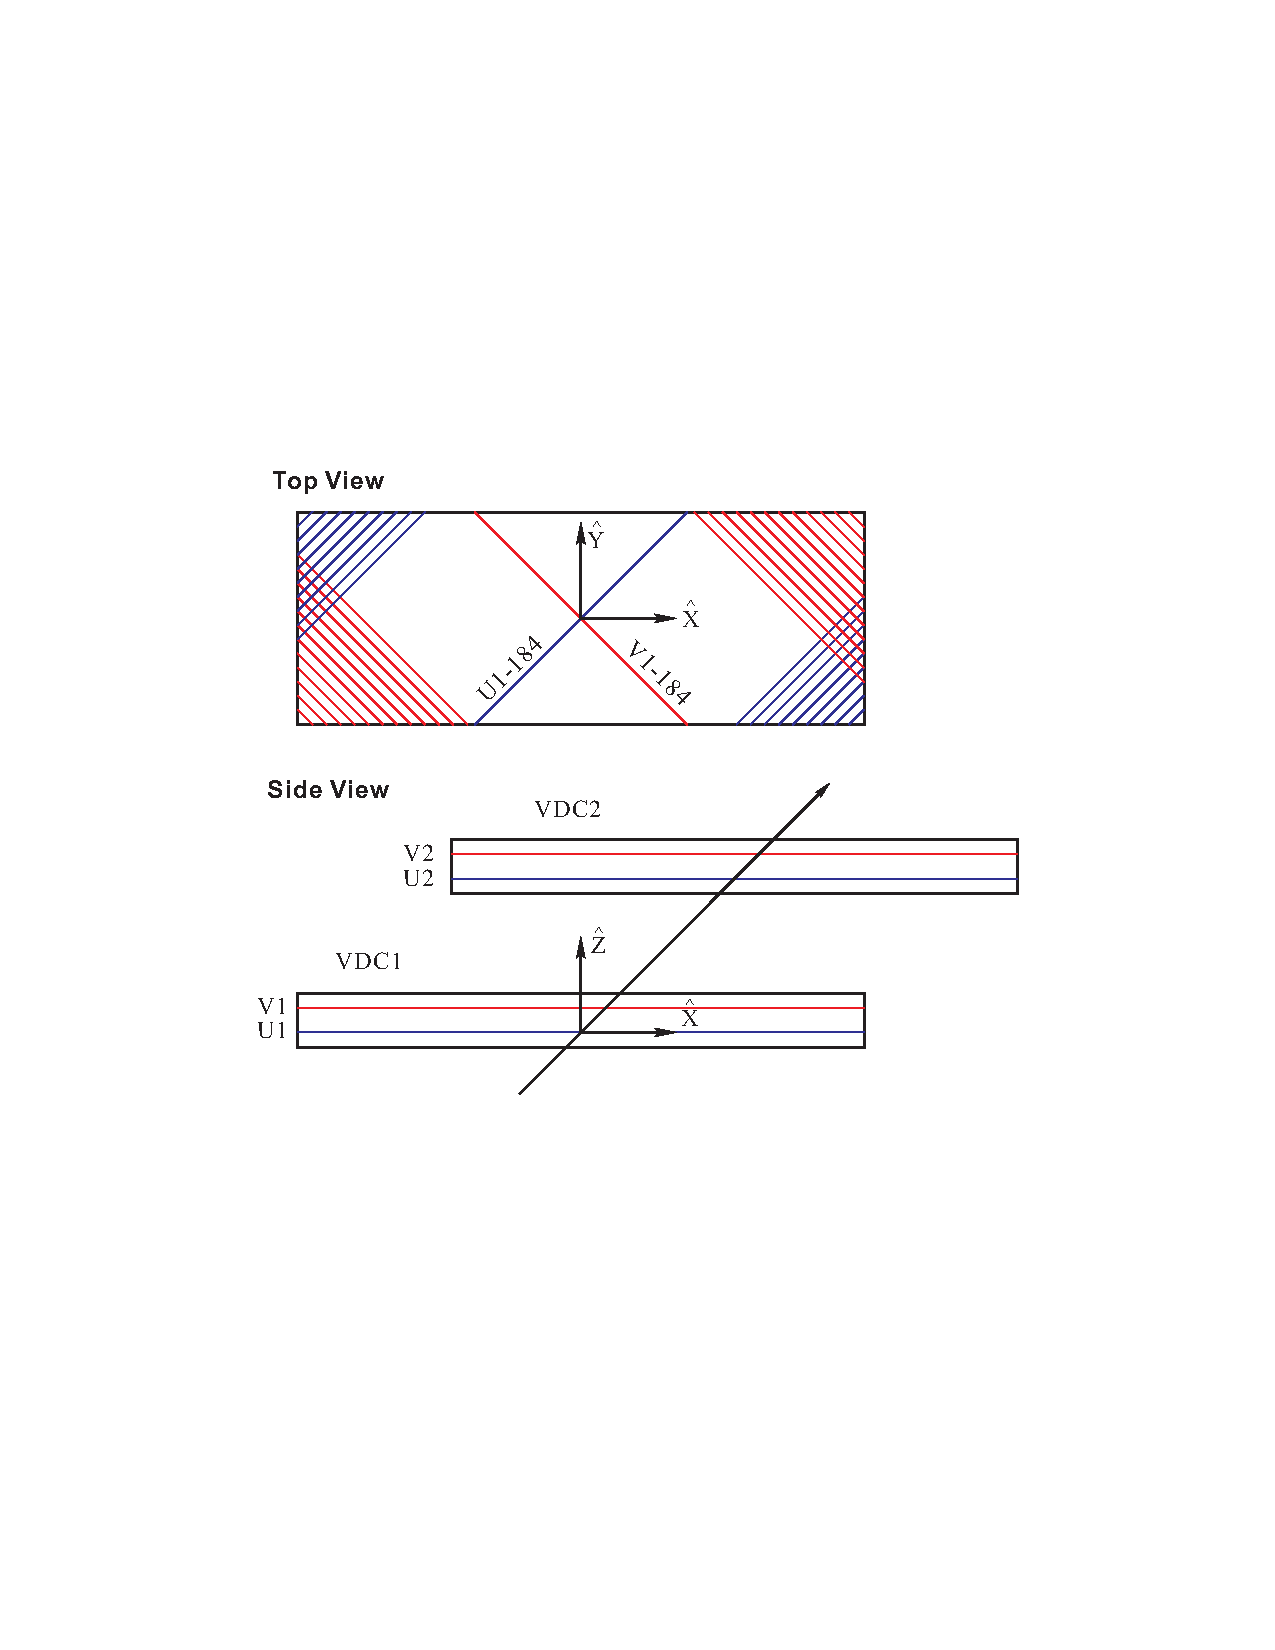
\includegraphics[width=0.75\textwidth]{figs/DCS.pdf}
  \caption[Detector coordinate system.]{Detector coordinate system (top and side views). The intersection point of the wire 184 of the U1 plane and the perpendicular projection of wire 184 of the V1 plane onto the U1 plane is shown in the top view. Plot reproduced from \cite{Qiang2007}. \label{C6S1SS3F1}}
\end{figure}

The coordinates of the detected particles are measured by the VDCs, as described in \Cref{C5}. The origin of the DCS is given by the intersection point of wire 184 of the VDC1 U1 plane and the perpendicular projection of wire 184 in the VDC1 V1 plane onto the VDC1 U1 plane. $\hat{z}_{\mathrm{det}}$ is perpendicular to the VDC plane pointing vertically up, and the $\hat{x}_{\mathrm{det}}$ is parallel to the long symmetry axis of the lower VDC pointing downstream. Thus the $\hat{y}_{\mathrm{det}}$ is parallel to the short symmetry axis of the lower VDC. See \Cref{C6S1SS3F1}. When a particle is detected, two spatial coordinates $\optx{det}$, $\opty{det}$ and two angular coordinates $\optt{det}\equiv\mathrm{d}x_{\mathrm{det}}/\mathrm{d}z_{\mathrm{det}}$, $\optp{det}\equiv\mathrm{d}y_{\mathrm{det}}/\mathrm{d}z_{\mathrm{det}}$ are calculated in this coordinate system.

\subsection[Transport Coordinate System at the Focal Plane]{Transport Coordinate System (TRCS) at the Focal Plane}
\label{C6S1SS4}

The TRCS at the focal plane is given by rotating the DCS around the $y$ axis by \SI{45}{\degree} clockwise if viewing along $y$ axis. Ideally, the $\hat{z}_{\mathrm{tra}}$ coincides with the central ray of the spectrometer. Typically, it is used to transport the DCS to the focal plane coordinate system. The TRCS coordinates of an event can be calculated from the DCS coordinates by:
\begin{align} \label{C6S1SS4E1}
\optx{tra} & = \optx{det}\cos(\rho_0)(1+\optt{tra}\tan(\rho_0)), \displaybreak[0] \\ \label{C6S1SS4E2}
\optt{tra} & = \frac{\optt{det}+\tan(\rho_0)}{1-\optt{det}\tan(\rho_0)}, \\  \label{C6S1SS4E3}
\opty{tra} & = \opty{det}+\sin(\rho_0)\optp{tra}\optx{det}, \\ \label{C6S1SS4E4}
\optp{tra} & = \frac{\optp{det}}{\cos(\rho_0)(1-\optt{det}\tan(\rho_0))},
\end{align}
where $\rho_0=-$\SI{45}{\degree}.

\subsection[Focal Plane Coordinate System]{Focal Plane Coordinate System (FCS)}
\label{C6S1SS5}

\begin{figure}[b!]
  \centering
  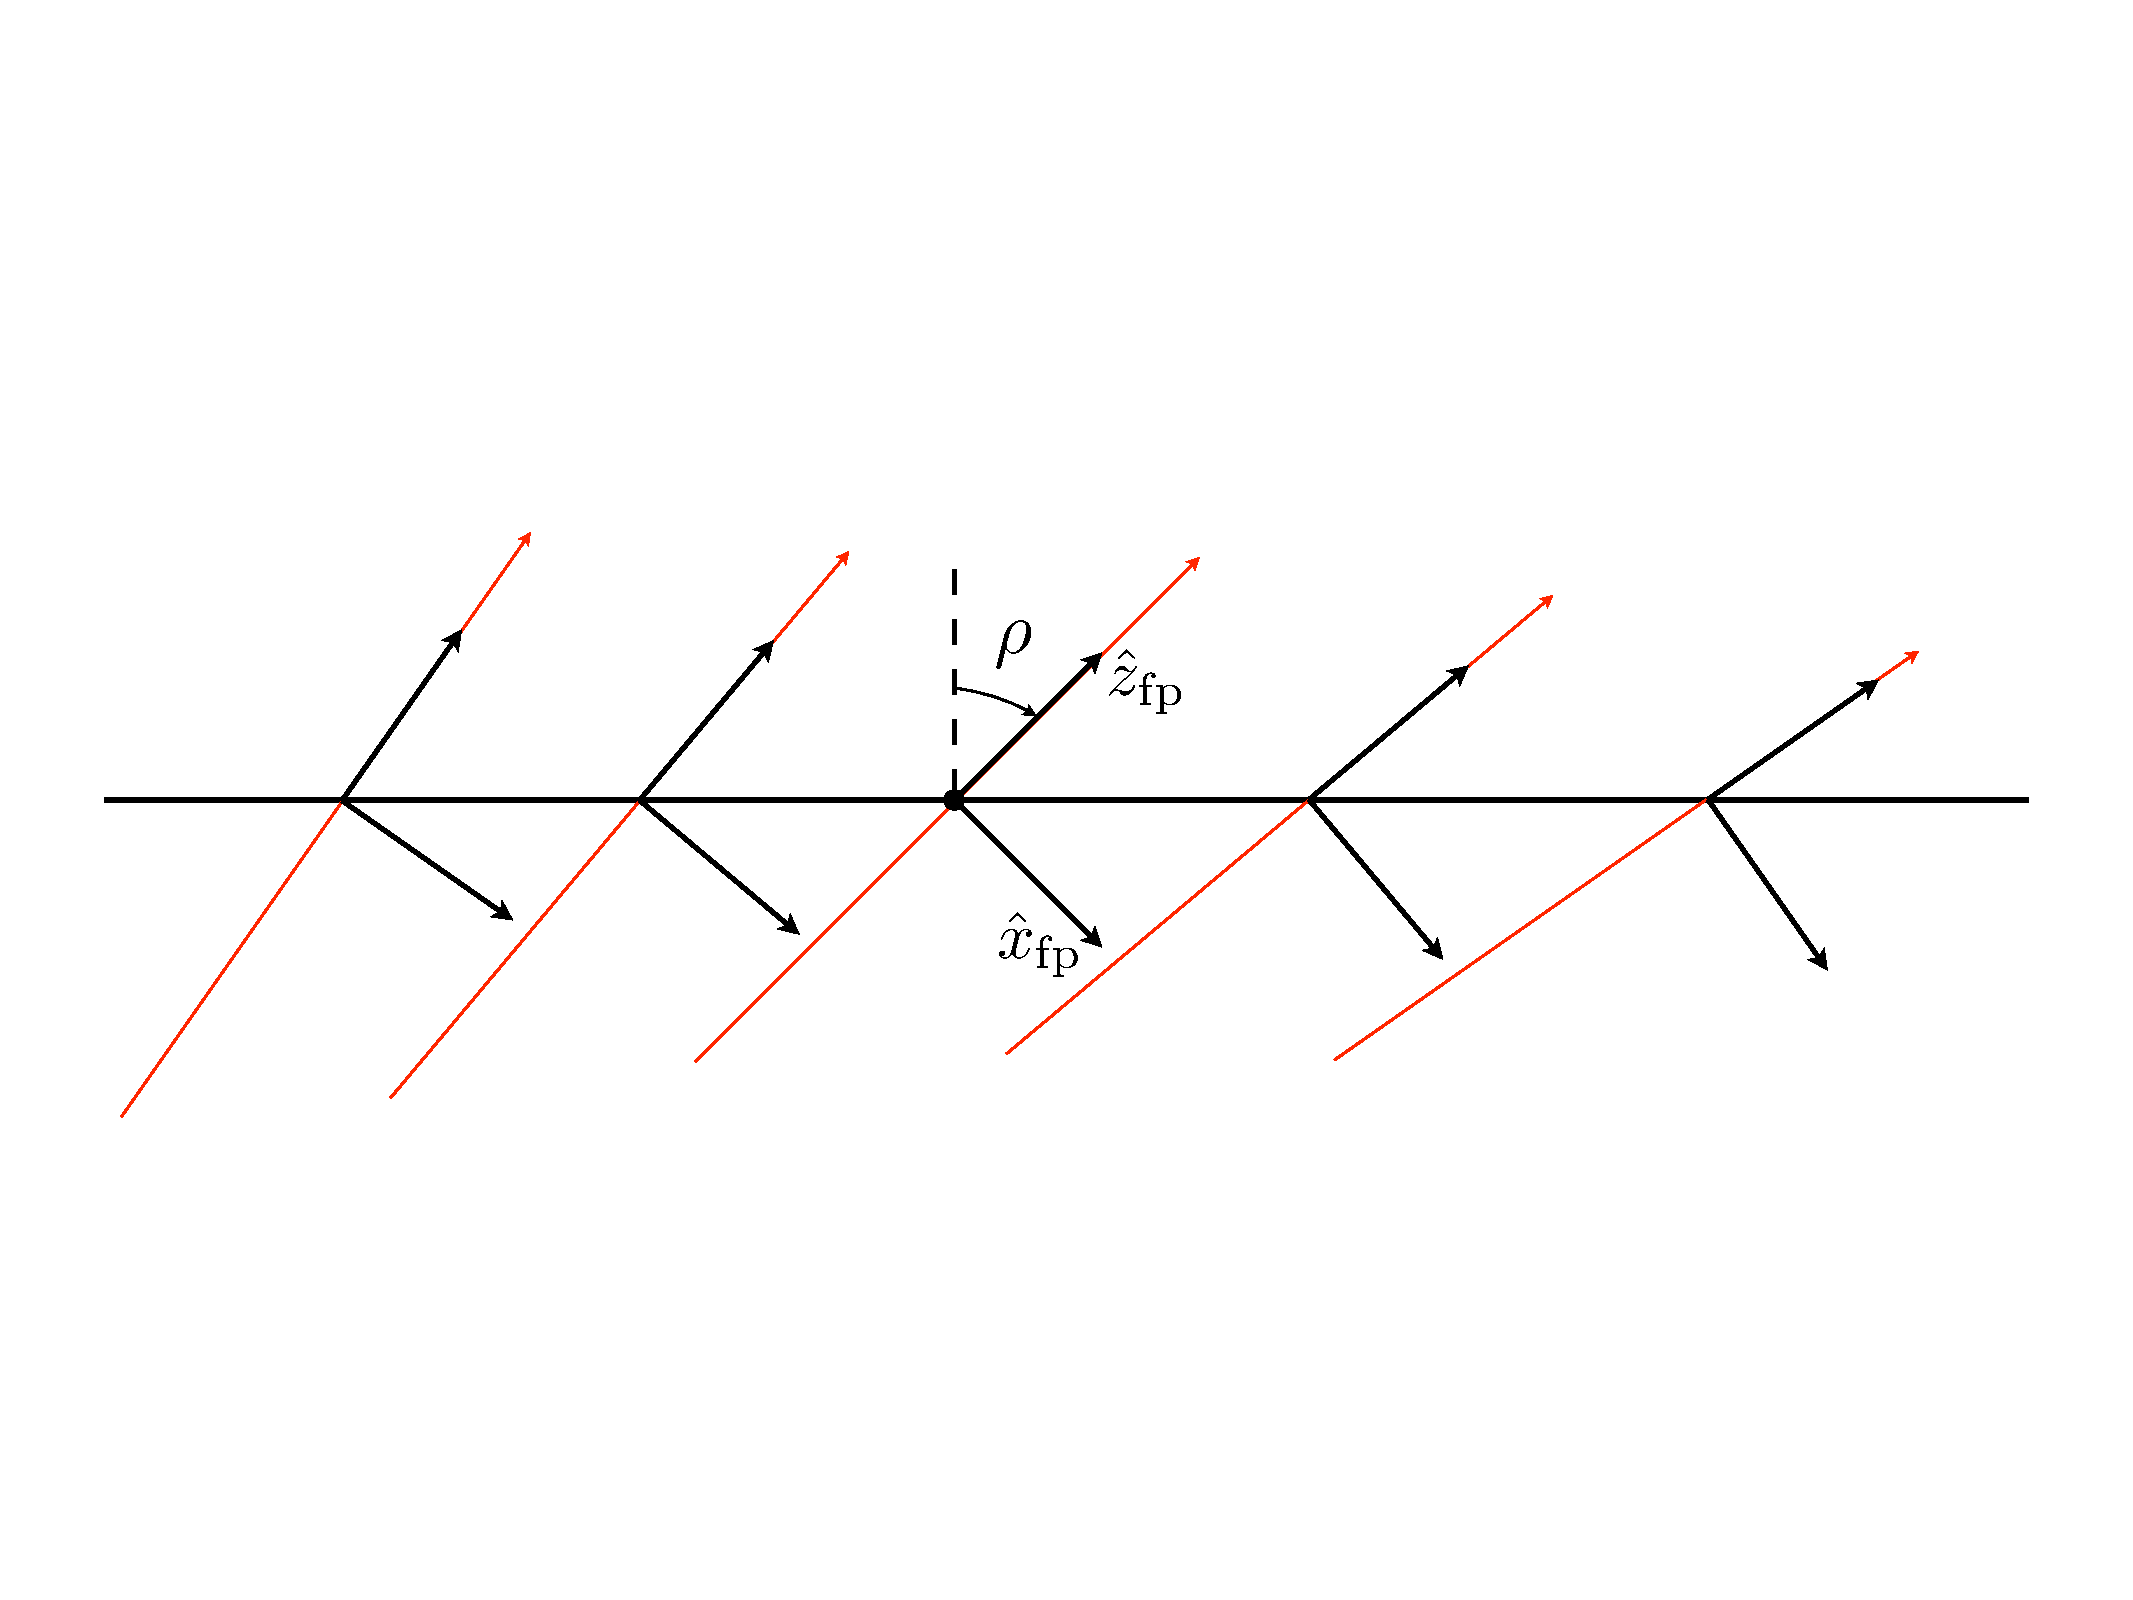
\includegraphics[width=0.7\textwidth]{figs/FCS.pdf}
  \caption[Focal plane coordinate system.]{Focal plane coordinate system. The red trajectories are the local certral rays with $\optt{tg}=\optp{tg}=0$. \label{C6S1SS5F1}}
\end{figure}

The FCS is a rotated coordinate system with its $z$ axis always parallel to the local central ray, which is defined as the trajectory of a particular particle with $\optt{tg}=\optp{tg}=0$ in the TCS for each relative momentum. This coordinate system is generated by rotating the DCS clockwise around its $y$ axis by the angle $\rho$ between the local central ray and the $z$ axis of the DCS. See \Cref{C6S1SS5F1}. Because of the focusing of the HRS magnet system, particles with the same scattering momentum will be focused at the focal plane, which means the relative momentum to the central momentum of the spectrometer is approximately a function of $\optx{tra}$. Therefore, the rotating angle $\rho$ is a function of $\optx{tra}$. As a result, the dispersive angle $\optt{fp}$ is small for all points across the focal plane in this rotated coordinate system, thus the expansion of the optics matrix will converge faster during the calibration, which will greatly simplify the optimizing procedure. The FCS coordinates of an event can be calculated form the DCS and TRCS coordinates by:
\begin{align} \label{C6S1SS5E1}
\optx{fp} & = \optx{tra} \\ \label{C6S1SS5E2}
\optt{fp} & = \frac{\optt{det}+\tan(\rho)}{1-\optt{det}\tan(\rho)} \\ \label{C6S1SS5E3}
\opty{fp} & = \opty{tra}-\sum_i C_{i000}^{\,y} \optx{fp}^i \\ \label{C6S1SS5E4}
\optp{fp} & = \frac{\optp{det}-\sum_i C_{i000}^{\,p}\optx{fp}^i}{\cos(\rho)(1-\optt{det}\tan(\rho))},
\end{align}
where $\tan(\rho) = \sum C_{i000}^{\,t} \optx{fp}^i$. The coefficients $C_{i000}^{\,t}$, $C_{i000}^{\,y}$ and $C_{i000}^{\,p}$ also include corrections for the systematic offsets due to misalignment of VDC packages.

\section{Optimization Procedure}
\label{C6S2}

\subsection{Optics Matrix}
\label{C6S2SS1}

As mentioned above, the DCS coordinates $\optx{det}$, $\optt{det}$, $\opty{det}$, $\optp{det}$ are directly measured with the VDC package. The optics matrix method allows a unique one-to-one mapping between these variables and the TCS variables, $\optx{tg}$, $\optt{tg}$, $\opty{tg}$, $\optp{tg}$ and $\delta$.

 During the optics calibration, the $\optx{tg}$ is effectively set at zero, therefore the unknowns at the target are reduced to four: $\delta$, $\optt{tg}$, $\opty{tg}$, $\optp{tg}$. Thus, the optics matrix can be expressed as (in a first-order approximation):
\begin{equation} \label{C6S2SS1E1}
\left(
\begin{matrix} \delta \\ \theta \\ y \\ \phi \end{matrix}
\right)_{\mathrm{tg}} = \left(
\begin{matrix}
\left<\delta|x\right> & \left<\delta|\theta\right> & 0 & 0 \\
\left<\theta|x\right> & \left<\theta|\theta\right> & 0 & 0 \\
0 & 0 & \left<y|y\right> & \left<y|\phi\right> \\
0 & 0 & \left<\phi|y\right> & \left<\phi|\phi\right>
\end{matrix}
\right)
\left(\begin{matrix} x \\ \theta \\ y \\ \phi \end{matrix}
\right)_{\mathrm{fp}}.
\end{equation}

In practice, the matrix takes a more complicated form: a set of tensors $D_{jkl}$, $T_{jkl}$, $Y_{jkl}$ and $P_{jkl}$, which are polynomials of $\optx{fp}$, links the FCS coordinates to TCS coordinates for each target variables. For example:
\begin{gather} \label{C6S2SS1E2}
\optt{tg} = \sum_{j,k,l} T_{jkl} \optt{fp}^j \opty{fp}^k \optp{fp}^l, \\ \label{C6S2SS1E3}
T_{jkl} = \sum_i C_{ijkl}^{T} \optx{fp}^i,
\end{gather}
where $C_{ijkl}^{T}$ are the optics matrix elements for $\optt{tg}$. Similar expressions can be written for $\delta$, $\opty{tg}$ and $\optp{tg}$. The summation over $i$, $j$, $k$ and $l$ is carried out and optimized up to the third order. The main purpose of the optimization procedure is to determine all optics matrix elements using dedicated optics calibration data, described in the next section.

\subsection{Matrix Optimization without Target Field}
\label{C6S2SS2}

The optics optimization procedure is always performed on a set of data with wide coverage on the entire acceptance of the spectrometer, which includes $\delta$ for momentum, $\optt{tg}$ and $\optp{tg}$ for solid angle and $\opty{tg}$ for reaction position. The target variables $\delta$, $\optt{tg}$, $\opty{tg}$ and $\optp{tg}$ for the calibration data set has to be precisely known. This requirement can be fulfilled by using survey results combined with a sieve-slit collimator for $\optt{tg}$ and $\optp{tg}$ and a foil target for $\opty{tg}$ and some well-known physics process like elastic scattering for $\delta$ as explained in this section.

\begin{figure}[tb!]
  \centering
  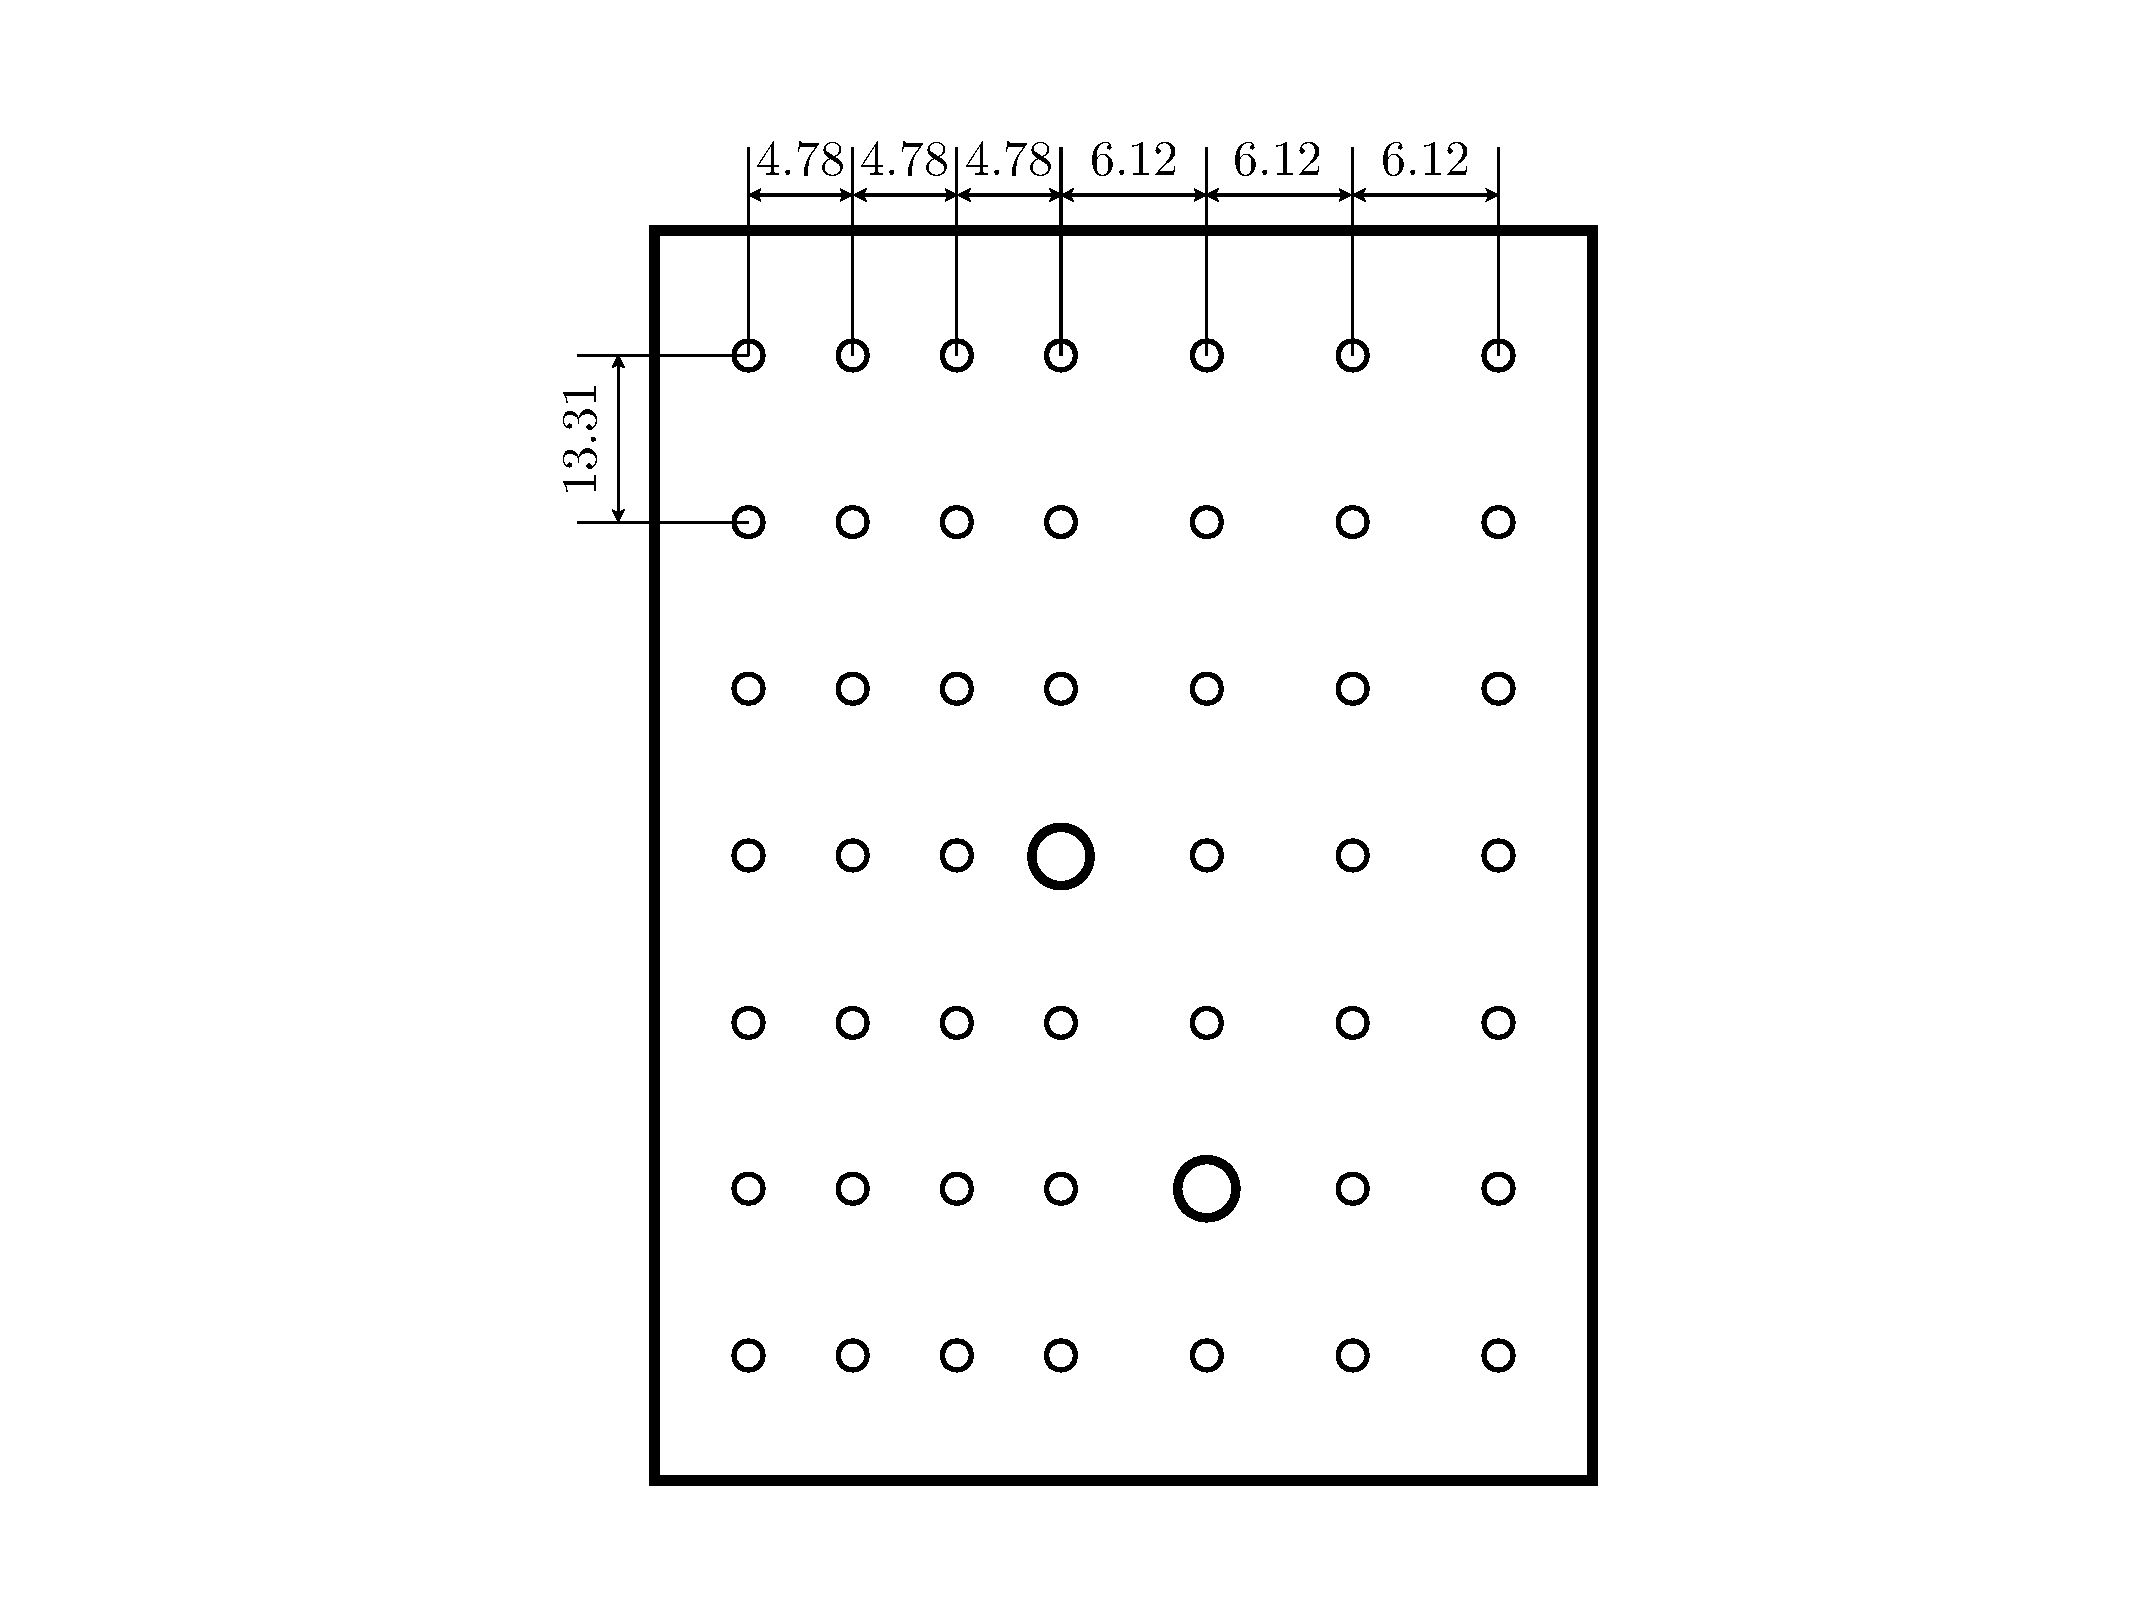
\includegraphics[width=0.3\textwidth]{figs/sieve-slit.pdf}
  \caption[Geometric configuration of the sieve slit.]{Geometric configuration of the sieve slit used during E08-027. The dimensions are in mm. The two large holes are used to determine the orientation of the sieve slit. The diameters are 1.4 mm and 2.7 mm for the normal holes and the large holes, respectively. \label{C6S2SS2F1}}
\end{figure}

To calibrate $\optt{tg}$, $\optp{tg}$ and $\opty{tg}$, a fixed energy electron beam with a point-like profile is incident on a set of foil target. The target foils are aligned along the beam line to cover the $\opty{tg}$ acceptance. Therefore, the HCS coordinates $\optx{beam}$ and $\opty{beam}$ of the interaction point can be determined by BPM, and the $z$ coordinate $\optz{react}$ can be determined by the survey result of the target foil. On the other side, a sieve slit collimator is placed before the entrance of the spectrometer (if there is a septum magnet, it is placed before the entrance of the septum magnet). A figure of the sieve slit used in E08-027 is shown in \Cref{C6S2SS2F1}. The sieve has holes that are arranged in a grid pattern with well-defined horizontal and vertical coordinates $\optx{sieve}$ and $\opty{sieve}$ (in TCS) covering the angular acceptance. The in-plane angle $\optp{tg}$ and the out-of-plane angle $\optt{tg}$ for each hole can be expressed as:
\begin{align} \label{C6S2SS2E1}
\optt{tg} & = \frac{\optx{sieve}+D_x+\opty{beam}}{L-\optz{react}\cos(\theta_0)-\optx{beam}\sin(\theta_0)}, \\ \label{C6S2SS2E2}
\optp{tg} & = \frac{\opty{sieve}+D_y-\optx{beam}\cos(\theta_0)+\optz{react}\sin(\theta_0)}{L-\optz{react}\cos(\theta_0)-\optx{beam}\sin(\theta_0)},
\end{align}
where $\theta_0$ is the spectrometer central angle, $L$ is the distance from the sieve slit to the TCS origin and the $D_x$ and $D_y$ are the vertical and horizontal deviations of the spectrometer central ray from the HCS origin, respectively, see \Cref{C6S1SS2F1}. $L$, $D_x$ and $D_y$ can be determined by surveying the spectrometer. The spectrometer central angle $\theta_0$ can be calculated from the geometries of the sieve slit and the target or by performing a pointing measurement using the energy deviation between the elastic peaks of two different nuclei \cite{Liyanage2011}. Precise determination of $\optt{tg}$ and $\optp{tg}$ is important because they determine the scattering angle via \cref{C6S1SS2E2}. With $\optt{tg}$ and $\optp{tg}$ known from \cref{C6S2SS2E1,C6S2SS2E2}, the spatial coordinates $\optx{tg}$ and $\opty{tg}$ can be expressed as:
\begin{align} \label{C6S2SS2E3}
\optx{tg} & = \optx{sieve}-L\optt{tg}, \\ \label{C6S2SS2E4}
\opty{tg} & = \opty{sieve}-L\optp{tg}.
\end{align}

To calibrate $\delta$, some well-known physics process can be used to determine the momentum of the detected particle. Take elastic scattering as example, the scattering momentum can be expressed as:
\begin{equation} \label{C6S2SS2E5}
P(M,\theta) = E' = \frac{E}{1+E/M(1-\cos(\theta))},
\end{equation}
where $E$ is the beam energy, $M$ is the target mass and $\theta$ is the scattering angle. Therefore, the target variable $\delta$ can be obtained from the calculated $P$ and the spectrometer central momentum $P_0$ by \cref{C6S1SS2E1}. To cover the acceptance range of $\delta$ of the HRS, several different $P_0$ values are used during the data collection to perform a so-called ``delta scan''. The energy loss of the scattered electrons due to the radiative effect when the electrons pass through the target material is considered as a correction to $\delta$.

As described above, the target variables $\optt{tg}$, $\opty{tg}$, $\optp{tg}$ and $\delta$ calculated from survey results (\cref{C6S2SS2E1,C6S2SS2E2,C6S2SS2E3,C6S2SS2E4}) or elastic scattering conditions (\cref{C6S2SS2E5}) are assumed to be the true value of the events in the data set collected with the sieve slit or elastic scattering. The optics matrix elements are then obtained by the minimizing of the aberration functions:
\begin{equation} \label{C6S2SS2E6}
\Delta (W) = \sum_s\left[\frac{\sum_{ijkl}C_{ijkl}^{W}\optx{fp}^i\optt{fp}^j\opty{fp}^k\optp{fp}^l-W^{0}}{\sigma_W^s}\right]^2,
\end{equation}
where $s$ is the total number of the events measured for optics calibration, $W$ can be any target variables $\delta$, $\optt{tg}$, $\opty{tg}$ or $\optp{tg}$ and $W_0$ is the corresponding reference variable calculated from survey results and the elastic condition. A C++ package based on the Hall A Analyzer \cite{Hansen2015} is developed to do this optimization, which is adopted from N. Liyanage's original code \cite{Liyanage2002} for ESPACE \cite{ESPACE}. The core of this package is the MIGRAD algorithm in the TMinuit package of ROOT \cite{ROOT}. The magnetic field simulation package SNAKE is used to generate an initial optics matrix for the optimization. This initial optics matrix accounts for the effects of the HRS magnets and the septum magnet. The package also contains a script for users to select events for optimization and some test scripts to compare the survey calculations with the reconstructed target variables.

\subsection{Target Field Effect}
\label{C6S2SS3}

As mentioned in \Cref{C5S3}, the field used to polarize the NH${}_3$ target is provided by a superconducting magnet, formed by a pair of Helmholtz coils. The field map of these coils has been directly calculated using the Biot-Savart law using the current density distribution of these coils. To estimate the uncertainty of this calculation, a measurement of the target field was performed during the experiment. The results indicate that the relative uncertainty of this field map is less than 1.2\% over the whole field region. The details of the field map are discussed in \Cref{A2}. The field map is calculated under the 5.0 T case and is scaled by 0.5 for the 2.5 T configuration.

The most important step during the optimization procedure in \Cref{C6S2SS2} is to determine the target plane variables for events collected during calibration runs. If there is no target field, the calculation of these variables only involves the linear projection between the sieve and the target and is straight forward. However, the linear projection is broken by the target field since the trajectory of the scattered electron is now a curve in the presence of this field.

A simulation package was developed to study the behavior of the scattered electrons in the target field. In order to do this, the equation of motion of the scattered electrons is integrated in the target field. The package uses the Runge-Kutta-Nystrom (RKN) method to do the integration. The trajectory of the electrons is approximated by chords in the integration method. For each chord, the deviation between its middle point and the real curve is also estimated by RKN method. The step size of the integration is adjusted dynamically to limit the integration uncertainty to $\leq$0.5 mm.

The trajectory of the scattered electron is also affected by the radiation effects when target field exists. The momentum of the electron decreases during the motion due to the energy loss. If there is no target field, the linear projection would not be influenced by the decreased momentum, but the curved trajectory of the scattered electron in the presence of the target field might change. This effect is also calculated in the simulation package. More details of the radiation effects can be found in reference \cite{Liu2015}.

With the help of the simulation package, the motion of the scattered electron in the target field region can be isolated. Since the field strength drops to less than 10 Gauss by the middle of the sieve slit, the sieve slit is taken as the edge of the target field region. Thus, the motion is separated into two parts: the first segment is from the interaction point to the sieve slit, where the trajectory can be calculated from the equation of motion, and the second segment is from the sieve slit to the focal plane, which can be described by the optics matrix.

\subsection{Matrix Optimization Revised}
\label{C6S2SS4}

The original optimization procedure had to be modified due to the presence of the target field. The reference values $W_0$ in \cref{C6S2SS2E6} can not be directly calculated from the survey results in this case. The new reference values are determined using the simulation package. The procedure to calculate new reference values involves the following steps:
\begin{enumerate}[parsep=0pt]
\item Select an elastic event, determine the coordinates of its interaction point ($\optx{react}$, $\opty{react}$, $\optz{react}$) and the coordinates of the sieve hole which it passes through ($\optx{sieve}$, $\opty{sieve}$);
\item Randomly generate a pair of scattering angles in TCS ($\optt{test}$, $\optp{test}$) and use \cref{C6S1SS2E2,C6S2SS2E5} to calculate the momentum $P_{\mathrm{elastic}}$ of the elastically scattered electron with this scattering angle;
\item \label{C6S2SS4A1} Set ($\optx{beam}$, $\opty{beam}$, $\optz{react}$) as start point and set $P_{\mathrm{elastic}}$ and ($\optt{test}$, $\optp{test}$) as the magnitude and direction of the momentum respectively, use the simulation package to generate a trajectory from the start point to sieve slit, assuming the coordinates of the intersection point of this trajectory and the sieve slit are ($\optx{drift}$, $\opty{drift}$);
\item \label{C6S2SS4A2} Compare ($\optx{drift}$, $\opty{drift}$) with ($\optx{sieve}$, $\opty{sieve}$), calculate the new test scattering angle:
\begin{align} \label{C6S2SS4E1}
\optt{test}^{\,\mathrm{new}} & = \optt{test}^{\,\mathrm{old}}+\frac{(\optx{drift}-\optx{sieve})/L}{2}, \\ \label{C6S2SS4E2}
\optp{test}^{\,\mathrm{new}} & = \optp{test}^{\,\mathrm{old}}+\frac{(\opty{drift}-\opty{sieve})/L}{2},
\end{align}
where $L$ is the distance from the sieve slit to the TCS origin;

\begin{figure}[tb!]
  \centering
  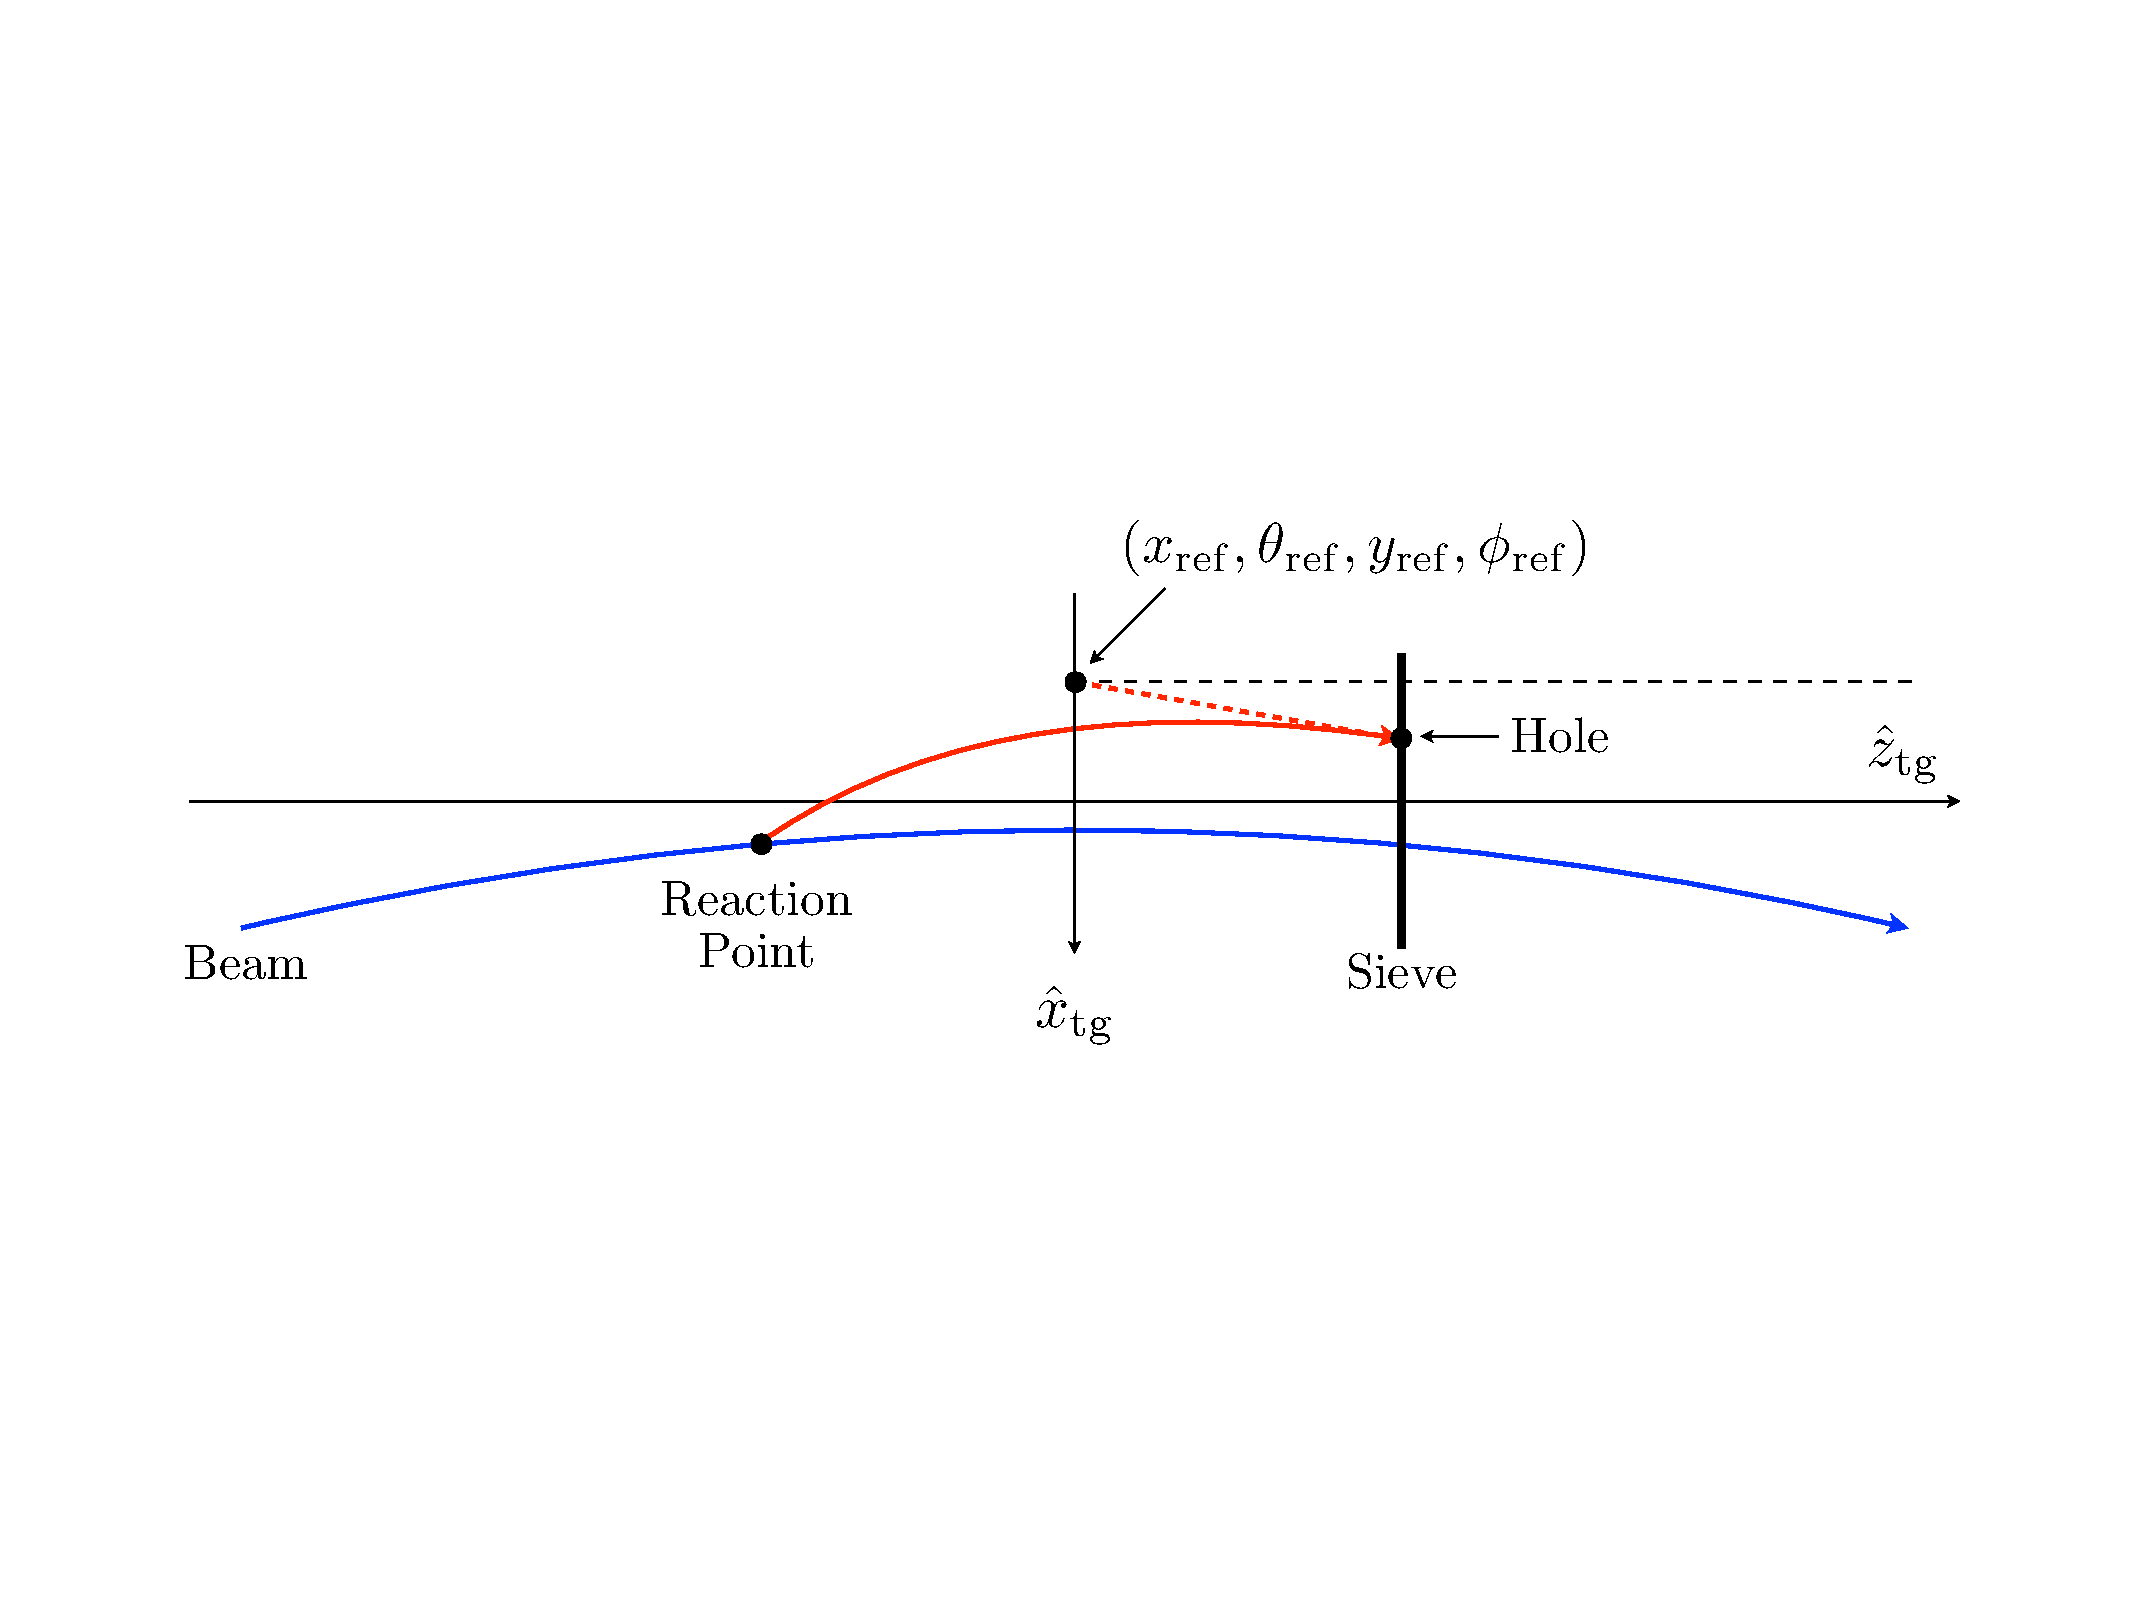
\includegraphics[width=0.9\textwidth]{figs/optics-reference-value.pdf}
  \caption[Determine the new reference values for the optics optimization.]{Determine the new reference values for the optics optimization with simulation. The red trajectory is determined in step \ref{C6S2SS4A1} and \ref{C6S2SS4A2}. \label{C6S2SS4F1}}
\end{figure}

\item Repeat step \ref{C6S2SS4A1} and \ref{C6S2SS4A2} until the deviation between the simulated point ($\optx{drift}$, $\opty{drift}$) and the actual sieve hole position ($\optx{sieve}$, $\opty{sieve}$) is less than the preset tolerance;
\item The trajectory obtained in the final step passes the interaction point and the same sieve hole as the electron passes, step \ref{C6S2SS4A1} assures it simulates an elastic electron. Thus it is the ideal trajectory for this particular event. If the coordinates of this trajectory at its intersection point with the sieve slit is defined as ($\optx{drift}$, $\optt{drift}$, $\opty{drift}$, $\optp{drift}$), the new reference values for the optimization can be obtained by projecting them to the target plane linearly, see \Cref{C6S2SS4F1}:
\begin{align} \label{C6S2SS4E3}
\optx{ref} & = \optx{drift}-L\optt{drift}, & \optt{ref} & = \optt{drift}, \\ \label{C6S2SS4E4}
\opty{ref} & = \opty{drift}-L\optp{drift}, & \optp{ref} & = \optp{drift}.
\end{align}
\end{enumerate}

Once the new reference values are determined, the same algorithm in \cref{C6S2SS2} can be used to do the optimization. A set of Python scripts is added into the original optimization package to calculate the reference values from the survey results with the simulation package. The optimization package is also updated to replace the linear-projected reference values with the new values from the simulation.

\section{Experimental Technique and Results}
\label{C6S3}

\subsection{Required Data}
\label{C6S3SS1}

\Cref{C5T1} summarizes the beam energy and the target field configuration for all kinematic settings. Unfortunately, the septum magnet coils for the right arm of the HRS burned twice during the experiment. Some turns of the coils in the septum were bypassed to fix it, which led to three different septum configurations. They are labeled by the number of the coil turns: ``48-48-16'' for the original septum, ``40-32-16'' for the septum burned once and ``40-00-16'' for the worst case. The septum configuration for each kinematic setting is listed in the septum column of \cref{C5T1}.

The polarized NH${}_3$ target need to be cooled down to 1K in a liquid He (LHe) bath. The LHe container is a cylinder and the diameter is only 42.0 mm. The length of the target is limited by the LHe container to only 28.3 mm along $z$ axis in the HCS. As mentioned in \cref{C6S2SS2}, a set of foil targets is generally used to cover the $\opty{tg}$ acceptance. But at \SI{5.77}{\degree}, the typical position resolution of $\opty{tg}$, $\approx$ 1 mm \cite{Alcorn2004}, is magnified by a factor of 10 in the position along the beam line ($z$ axis in the HCS), which means that the multiple foils installed in the 28.3 mm target cell can not be easily distinguished by the spectrometer. Thus, only one carbon foil is used to collect optics data and we can only optimize $\delta$, $\optt{tg}$ and $\optp{tg}$. The BPM readout is used to determine $y_{tg}$ instead without optics calibration. The thickness of the carbon foil was 40 mil (1.016 mm) for settings 1-5 in \cref{C5T1} and 125 mil (3.175 mm) for the other settings. The foil locations along the beam direction ($\optz{react}$ in \cref{C6S2SS2E1,C6S2SS2E2}) was -13.6 mm for settings 1-5 in \cref{C5T1} and -12.5 mm for the other settings. To reduce the radiation effect, the LHe in the LHe container was vapored and pumped out when collecting the optics data.

The sieve slit used to take optics data is shown in \Cref{C6S2SS2F1}. There are 49 holes in a 7$\times$7 grid pattern with two holes larger than the others. The large holes are used to determine the orientation of the image of the sieve slit. The horizontal distance between the four columns closest to the beam is larger than the distance between the other three columns. This can also be used to determine the orientation in the image. The survey information of the sieve slit was used to calculate the offsets of the central hole from its ideal positions. The $\optx{sieve}$ and $\opty{sieve}$ for each sieve hole is calculated from these offsets and the relative position to the center of the sieve slit. As calculated from the survey result \cite{SurveyA1453,SurveyA1465}, the horizontal offset $D_y$ is 0.0 mm and the vertical offset $D_x$ is -0.2 mm.

The beam position $\optx{beam}$ and $\opty{beam}$ is determined by BPMs. The details of the calibration of the BPMs can be found in reference \cite{Zhu2016}. Because of the target field, the beam is not a straight line in this experiment. The incident angle of the beam at the target can be obtained from the BPM readouts, which can be expressed as the polar angle $\optt{beam}$ and the azimuthal angle $\optp{beam}$ in the HCS. The scattering angle is the angle between the incident beam and the trajectory of the scattered electron, which can be calculated via two auxiliary vectors. The vector describing the beam direction is:
\begin{equation} \label{C6S3SS1E1}
\vec{A} = (\sin(\optt{beam})\cos(\optp{beam}),\ \sin(\optt{beam})\sin(\optp{beam}),\ \cos(\optt{beam})),
\end{equation}
while the vector corresponding to the scattered electron is:
\begin{equation} \label{C6S3SS1E2}
\vec{B} = (\optp{tg}\cos(\theta_0)+\sin(\theta_0),\ -\optt{tg},\ \cos(\theta_0)-\optp{tg}\sin(\theta_0)),
\end{equation}
and the scattering angle is determined as:
\begin{equation} \label{C6S3SS1E3}
\cos\optt{scat} = \frac{\vec{A}\cdot\vec{B}}{|\vec{A}||\vec{B}|},
\end{equation}
where $\optt{beam}$ and $\optp{beam}$ are the azimuthal angles of the incident angle of the beam and $\optt{tg}$ and $\optp{tg}$ are the tangents of the corresponding angles to keep consistent with the definition in the TCS. \cref{C6S3SS1E1,C6S3SS1E2,C6S3SS1E3} replace \cref{C6S1SS2E2} when the beam has an incident angle.

Delta scan was performed by setting $P_0$ at $\pm 3\%$, $\pm 2\%$, $\pm 1\%$ and $0\%$ of the elastic momentum for each configuration except for the one with 3.350 GeV beam energy. In this paticular setting, the elastic scattered electrons can not pass through the septum magnet even if the septum current is set to its upper limit. Since only one foil of carbon target is used in the experiment, the $\opty{tg}$ coverage of the optics calibration was limited. Thus, the incident beam position was adjusted manually by a few millimeters to perform a beam position scan to increase the $\opty{tg}$ coverage. Assuming that the original beam position is (0,0), beam position scan is performed at (0,$\ \pm 4$ mm) and ($\pm 4$ mm,0).

\subsection{Optimization Results}
\label{C6S3SS2}

The optics matrix was optimized for each beam energy and target field configurations listed in \cref{C5T1} except for 3.350 GeV. The procedure discussed in \cref{C6S2SS4} was followed. In this section, the event selection and optimization results are discussed. The data collected with the 1.710 GeV beam energy and 2.5 T transverse target field is taken as an example.

The spectrometer central angle needs to be determined before the matrix calibration. As mentioned in \Cref{C6S2SS2}, the pointing measurement is considered to be more accurate than a survey for the spectrometer central angle determination, since most of the systematic uncertainty can cancel out when considering the difference of the elastic peak. However, in this experiment, although the carbon and the LHe can be used to perform a pointing measurement, the systematic error can not cancel completely due to the fact that the center of the liquid helium region could not be determined accurately. Thus, the survey method was chosen to determine the spectrometer central angle. The result is summarized in \cref{C6S3SS2T1}. More details about the central angle calibration can be found in Ref. \cite{Huang2014}.

\begin{table}[tb!]
  \centering
  \newcolumntype{C}[1]{>{\centering\arraybackslash}m{#1}}
  \begin{tabular}{|c|C{2.5cm}|C{2cm}|}
    \hline
    Arm & Central Angle (rad) \\ \hline
    HRS-L & 0.1007$\pm$0.0007 \\ \hline
    HRS-R & 0.1009$\pm$0.0007 \\ \hline
  \end{tabular}
  \caption[Spectrometer central angles.]{Spectrometer central angles. \label{C6S3SS2T1}}
\end{table}

\begin{figure}[b!]
  \centering
  \begin{subfigure}[t]{0.49\textwidth}
    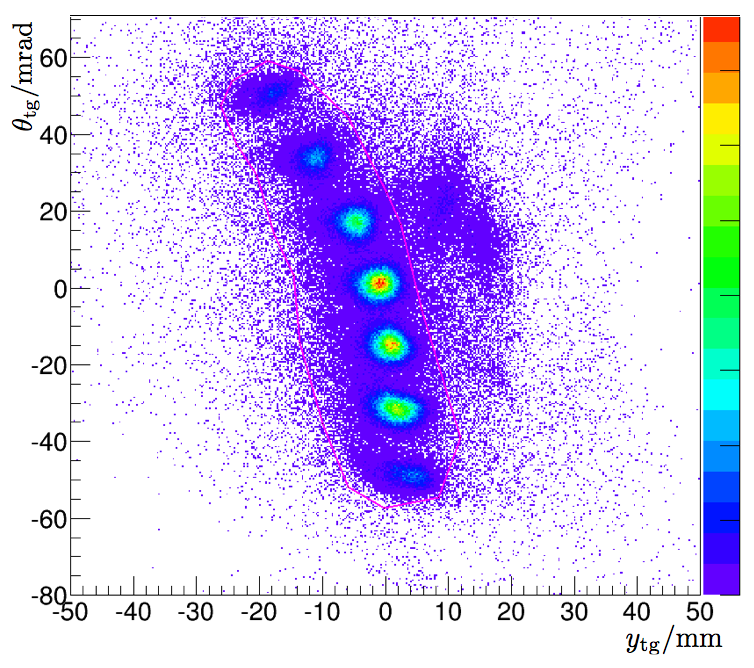
\includegraphics[width=\textwidth]{figs/foil-cut.png}
  \end{subfigure}
  \begin{subfigure}[t]{0.49\textwidth}
    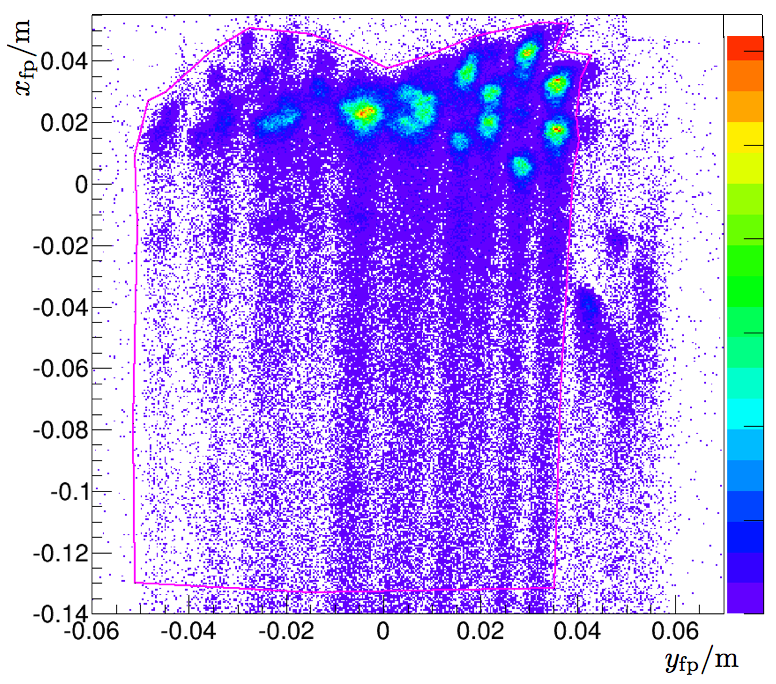
\includegraphics[width=\textwidth]{figs/focal-plane-cut.png}
  \end{subfigure}
  \caption[The foil cut and the focal plane cut.]{The foil cut (left) and the focal plane cut (right). \label{C6S3SS2F1}}
\end{figure}

Before the optics study, the initial matrix generated by SNAKE as mentioned in \cref{C6S2SS2} was used to reconstruct the target variables of the optics data. These target variables were used to make cuts. The data need to be selected by applying several different kinds of cut. Although the carbon foil data is relatively clean, it can still be diluted by electrons scattered from the windows on the target chamber. These events can be removed by applying a foil cut on $\opty{tg}$ or a cut on the focal plane variable $\opty{fp}$ since only one foil was used. The focal plane cut and $\opty{tg}$ cut are shown in \Cref{C6S3SS2F1}, which were chosen empirically. After the foil cut was made, a set of cuts on target variable $\optt{tg}$ and $\optp{tg}$ was made for each hole in the sieve slit. And for each sieve hole, a cut on relative momentum $\delta$ was made to select the elastic events. Since $\opty{tg}$ acceptance is covered by the beam position scan instead of using multiple foils of target, a beam position cut on $\optx{beam}$ and $\opty{beam}$ was also performed to select data with the proper beam position. The cut definition process was repeated for each delta scan and beam position scan configurations. Each cut was assigned with an identification number and saved to a separate file.

The optimization package uses the saved cuts to select events. The FCS coordinates, positions and angles of the beam and the identification number of the cut for selected events are recorded into a ASCII file. The script mentioned in \Cref{C6S2SS4} uses the file as an input to calculate the reference values for optimization, and append the reference values to the focal plane variables for each event in the file. For example, the reference values of $\optt{tg}$ and $\optp{tg}$ for 1.710 GeV configuration is shown in the left panel of \Cref{C6S3SS2F2}. The focal plane variables and the reference values are read by the updated optimization program from the file to optimize the optics matrix.

\begin{figure}[tb!]
  \centering
  \begin{subfigure}[t]{0.45\textwidth}
    \includegraphics[width=\textwidth]{figs/reference-angle-simulation.png}
  \end{subfigure}
  \begin{subfigure}[t]{0.45\textwidth}
    \includegraphics[width=\textwidth]{figs/initial-angle-simulation.png}
  \end{subfigure}
  \caption[Reference values for angular optimization.]{The reference values of $\optt{tg}$ and $\optp{tg}$ for optimization (left) and the corresponding actual target plane angle at the reaction point (right). The difference between the two panels is due to the target field, which was determined from the simulation described in \Cref{C6S2SS3}. \label{C6S3SS2F2}}
\end{figure}

\begin{figure}[b!]
  \centering
  \includegraphics[width=\textwidth]{figs/sieve-pattern.png}
  \caption[Sieve Pattern for 1.710 GeV data.]{Sieve Pattern for 1.710 GeV data. The patterns of different delta scans are shown in separate plots. The three plots in the top row is delta scans with spectrometer central momenta ($P_0$) setting to $+3\%$ (left), $+2\%$ (center) and $0\%$ (right) of the elastic momentum, the bottom row is delta scans with $P_0$ setting to $-2\%$ (left) and $-3\%$ (center). The cross points of the grids in the plots are used to indicate the actual positions of the sieve holes. The good agreement between the hole images and the grid indicates the angles $\optt{tg}$ and $\optp{tg}$ have been calibrated well. \label{C6S3SS2F3}}
\end{figure}

The angular components of the optics matrix are optimized first. The optimized matrix is used to reconstruct the target variables. The sieve pattern is generated by the projection of the reconstructed $\optt{tg}$ and $\optp{tg}$ from the interaction point to the sieve slit plane. The sieve pattern for the 1.710 GeV data is shown in \Cref{C6S3SS2F3}. The nominal position of the sieve holes are indicated by the cross points of the grids in the plots.

\begin{figure}[tb!]
  \centering
  \includegraphics[width=0.6\textwidth]{figs/delta-pattern.png}
  \caption[The $\delta_{\mathrm{kin}}$ calibration results for 1.710 GeV data.]{The $\delta_{\mathrm{kin}}$ calibration results for 1.710 GeV data. The peaks in the plot are the reconstructed $\delta_{\mathrm{kin}}$ from different delta scan configurations, summed over all sieve holes. Starting from the left, the spectrometer central momenta are $+3\%$, $+2\%$, $0\%$, $-2\%$ and $-3\%$ of the elastic momentum respectively. The magenta lines in the plots indicate the actual value of the $\delta_{\mathrm{kin}}$. \label{C6S3SS2F4}}
\end{figure}

Next step is the momentum calibration. As shown in \cref{C6S2SS2}, the momentum of an elastically scattered electron depends on the scattering angle. Since the sieve slit covers a wide angle range, the scattering angles of the electrons passing through different sieve holes are different. The elastic peak is broadened due to this effect, which influences the resolution of the optimization. Thus, a new variable is defined to remove the angular dependence of $\delta$:
\begin{equation} \label{C6S3SS2E1}
\delta_{\mathrm{kin}} = \delta - \frac{P(M,\ \theta)-P(M,\, \theta_0)}{P_0},
\end{equation}
where $\theta_0$ is the spectrometer central angle and $\theta$ is the scattering angle. The second term on the right hand side of \cref{C6S3SS2E1} is defined as $\delta_{\mathrm{corr}}$:
\begin{equation} \label{C6S3SS2E2}
\delta = \delta_{\mathrm{kin}} + \delta_{\mathrm{corr}}(M, \theta).
\end{equation}
$\delta_{\mathrm{corr}}$ only depends on the target material and the scattering angle. In practice, $\delta_{\mathrm{corr}}$ is calculated with the survey result and the beam positions before the optimization starts. During the optimization, the saved $\delta_{\mathrm{corr}}$ can be used to convert $\delta$ to $\delta_{\mathrm{kin}}$ with almost no additional computing cost. Momentum $\delta_{\mathrm{kin}}$ for events from different sieve holes can then be optimized together. The $\delta_{\mathrm{kin}}$ calibration results for 1.710 GeV data are shown in \Cref{C6S3SS2F4}. The nominal positions of the $\delta_{\mathrm{kin}}$ are indicated by magenta lines for each delta scan configuration.

\begin{table}[tb!]
  \centering
  \newcolumntype{C}[1]{>{\centering\arraybackslash}m{#1}}
  \begin{tabular}{|c|C{2.2cm}|C{2.2cm}|}
    \hline
     & Left Arm & Right Arm \\ \hline
    $\delta_{\mathrm{res}}$ & 1.5$\times10^{-4}$ & 2.4$\times10^{-4}$ \\ \hline
    $\theta_{\mathrm{res}}$ (mrad) & 1.6 & 1.6 \\ \hline
    $\phi_{\mathrm{res}}$ (mrad) & 1.0 & 0.8 \\ \hline
  \end{tabular}
  \caption[Summary of the optics performance without target field.]{Summary of the optics performance without target field. $\delta_{\mathrm{res}}$, $\theta_{\mathrm{res}}$ and $\phi_{\mathrm{res}}$ are resolutions in $\delta$, $\theta$ and $\phi$, respectively. \label{C6S3SS2T2}}
\end{table}

\begin{table}[tb!]
  \centering
  \newcolumntype{C}[1]{>{\centering\arraybackslash}m{#1}}
  \begin{tabular}{|c|C{1.7cm}|C{1.7cm}|C{1.2cm}|c|c|C{1.2cm}|C{1.2cm}|}
    \hline
    HRS & Beam Energy (GeV) & Field Strength (T) & Field Angle & Septum & $\delta_{\mathrm{res}}$ & $\theta_{\mathrm{res}}$ (mrad) & $\phi_{\mathrm{res}}$ (mrad) \\ \hline
    L & 2.254 & 2.5 & \SI{90}{\degree} & 48-48-16 & 2.0$\times10^{-4}$ & 1.7 & 1.7 \\ \hline
    L & 2.254 & 2.5 & \SI{90}{\degree} & 40-32-16 & 2.2$\times10^{-4}$ & 1.8 & 1.8 \\ \hline
    L & 1.710 & 2.5 & \SI{90}{\degree} & 40-00-16 & 2.4$\times10^{-4}$ & 2.4 & 1.5 \\ \hline
    L & 1.157 & 2.5 & \SI{90}{\degree} & 40-00-16 & 3.2$\times10^{-4}$ & 2.1 & 1.3 \\ \hline
    L & 2.254 & 5.0 & \SI{0}{\degree} & 40-00-16 & 2.2$\times10^{-4}$ & 1.6 & 1.2 \\ \hline
    R & 2.254 & 2.5 & \SI{90}{\degree} & 48-48-16 & 1.8$\times10^{-4}$ & 1.6 & 1.2 \\ \hline
    R & 2.254 & 2.5 & \SI{90}{\degree} & 40-32-16 & 2.5$\times10^{-4}$ & 2.2 & 1.8 \\ \hline
    R & 1.710 & 2.5 & \SI{90}{\degree} & 40-00-16 & 2.3$\times10^{-4}$ & 2.7 & 1.7 \\ \hline
    R & 1.157 & 2.5 & \SI{90}{\degree} & 40-00-16 & 3.4$\times10^{-4}$ & 1.9 & 1.5 \\ \hline
  \end{tabular}
  \caption[Summary of optics performance with the target field.]{Summary of optics performance with the target field. Here ``L'' and ``R'' stand for the left arm and right arm of the HRS. $\delta_{\mathrm{res}}$, $\theta_{\mathrm{res}}$ and $\phi_{\mathrm{res}}$ are resolutions in $\delta$, $\theta$ and $\phi$, respectively. \label{C6S3SS2T3}}
\end{table}

In this section, only the optimization results for 1.710 GeV configuration is shown as an example. However the optimization was performed for all kinematic settings and the optics data without target field was optimized as well with the normal procedure to verify the HRS performance. The resolutions of the optics matrix without the target field is summarized in \cref{C6S3SS2T2} and the resolutions of the optics matrix with target field is summarized in \cref{C6S3SS2T3}. Here the resolution is evaluated via:
\begin{equation} \label{C6S3SS2E3}
f_{\mathrm{res}}^W = \sqrt{\frac{1}{N}\sum_{s=1}^N(W_s-W_s^0)^2},
\end{equation}
where $W$ are calculated with optics matrix, $W_0$ are the reference values and $N$ is the total number of the events used in the optimization. See Ref. \cite{OPTICSWIKI} for more plots of the optimization results for each setting listed in \cref{C5T1}.

\section{Reconstruction Procedure}
\label{C6S4}

Since the final purpose of the optics study is to reconstruct the kinematic variables for each event, the reconstruction procedure is included as part of the optics study. If there is no target field, the Hall A Analyzer is designed to read the optics matrix and calculate the target plane variables directly for each event \cite{Hansen2015} and no additional process is required. However, this is not the case with the target field.

\begin{figure}[b!]
  \centering
  \includegraphics[width=0.9\textwidth]{figs/reconstruction.pdf}
  \caption[Reconstruction of the target kinematic variables.]{Reconstruction of the target kinematic variables. Here $\optt{eff}$ is reconstrcted by the optics matrix from the focal plane variable. The red dot line shows the linear projection to the sieve slit plane and the read solid line indicates the trojectory generated by the simulation package, which gives us the real target variable $\optt{tg}$. The detailed procudure is discussed in this section.  \label{C6S4F1}}
\end{figure}

Following the logic in \Cref{C6S2SS4}, the reconstruction procedure can also be completed in two steps. The first step is to reconstruct the coordinates of the intersection point of the scattered electron and the sieve slit plane, which can be obtained from the focal plane variables with the optimized optics matrix. The second step is to determine the trajectory of the electron from the sieve slit plane to the target with the simulation package. The detailed procedure to reconstruct kinematic variables involve the following steps:
\begin{enumerate}[parsep=0pt]
\item \label{C6S4A1} Select an event, apply the optics matrix to the focal plane coordinates ($\optx{fp}$, $\optt{fp}$, $\opty{fp}$, $\optp{fp}$) to calculate the relative momentum $\delta$ and the effective target angles $\optt{eff}$ and $\optp{eff}$ at the target plane, which is the $z=0$ plane in TCS. In practice, this step is performed by the Hall A Analyzer;
\item \label{C6S4A2} Calculate the effective beam positions $\optx{eff}$ and $\opty{eff}$ in TCS from the actual beam positions provided by BPMs with the target field simulation described later. Combine with the angles obtained in step \ref{C6S4A1}, the effective target variables are ($\optx{eff}$, $\optt{eff}$, $\opty{eff}$, $\optp{eff}$);
\item Perform a linear projection of ($\optx{eff}$, $\optt{eff}$, $\opty{eff}$, $\optp{eff}$) to the sieve slit plane, which is the $z=L$ plane in TCS, to obtain ($\optx{proj}$, $\optt{proj}$, $\opty{proj}$, $\optp{proj}$);
\item Set ($\optx{proj}$, $\opty{proj}$, $\optz{proj}=L$) as the start point and set the $\delta$ and ($\optt{proj}$, $\optp{proj}$) as the magnitude and direction of the momentum respectively, use the simulation package to generate a trajectory from the start point to the target plane in TCS, which gives the target variables ($\optx{tg}$, $\optt{tg}$, $\opty{tg}$, $\optp{tg}$) of the selected event.
\end{enumerate}

\begin{figure}[b!]
  \centering
  \includegraphics[width=0.6\textwidth]{figs/effective-x-fit.png}
  \caption[Determine the effective beam position correction.]{The relation between $\optx{eff}-\optx{beam}$ and the momentum of the scattered electron from the simulation. The red curve is the fit result of the function in \cref{C6S4E1}. \label{C6S4F2}}
\end{figure}

\begin{table}[b!]
  \centering
  \newcolumntype{C}[1]{>{\centering\arraybackslash}m{#1}}
  \begin{tabular}{|C{1.2cm}|C{2.3cm}|C{1.8cm}|C{2.2cm}|C{1.8cm}|C{2.2cm}|}
    \hline
    HRS & Field & $C_0^{\,x}$ (mm) & $C_1^{\,x}$ (mm$\cdot$GeV/c) & $C_0^{\,y}$ (mm) & $C_1^{\,y}$ (mm$\cdot$GeV/c) \\ \hline
    Left & 2.5 T at \SI{90}{\degree} & 0.00 & 3.14 & -0.09 & 0.22 \\ \hline
    Left & 5.0 T at \SI{0}{\degree} & 0.00 & -0.75 & 0.16 & -0.40 \\ \hline
    Left & 5.0 T at \SI{90}{\degree} & -0.04 & 6.34 & -0.35 & 0.86 \\ \hline
    Right & 2.5 T at \SI{90}{\degree} & 0.00 & 3.13 & 0.09 & -0.21 \\ \hline
    Right & 5.0 T at \SI{0}{\degree} & 0.00 & 0.76 & -0.15 & 0.34 \\ \hline
    Right & 5.0 T at \SI{90}{\degree} & -0.05 & 6.37 & 0.35 & -0.85 \\ \hline
  \end{tabular}
  \caption[Fit parameters of effective beam position correction.]{Fit parameters of the effective beam position correction. \label{C6S4T1}}
\end{table}

The effective beam positions $\optx{eff}$ and $\opty{eff}$ used in step \ref{C6S4A2} is generated by adding a correction to actual position, $\optx{beam}$ and $\opty{beam}$, of the scattered electron. The correction is defined as $\optx{eff}-\optx{beam}$, which is plotted in \Cref{C6S4F2} for 2.5 T transverse target field setting as an example. Since the target in this experiment is short, the $\optx{eff}-\optx{beam}$ term is dominated by the deviation of the linear projection from the actual trajectory. The deviation shows a strong correlation with the momentum $P$ of the scattered electron due to the target field. The simulated $\optx{eff}-\optx{beam}$ values can be fit as a function of $P$:
\begin{equation} \label{C6S4E1}
\optx{eff}-\optx{beam} = C_0 + C_1/P.
\end{equation}
Similar expressions can be written for $\opty{eff}$ and $\opty{beam}$. The fit is performed for all three target field configurations on both spectrometers. The fit parameters are summarized in \cref{C6S4T1}.

A Python script was developed to calculate the kinematic variables following the procedure described above. The original reconstruction script based on the Hall A analyzer is included in this script as a preprocessor of the data.

%%%%%%%%%%%%%%%%%%%%%%%%%%%%%%%%%%%%%%%%%%%%%%%%%%%%%%%%%%%%%%%%%%%%%%
% -*-latex-*-

% -*-latex-*-

\chapter{Analysis}
\label{C7}

For E08-027, asymmetries and unpolarized cross-sections are measured to extract the polarized cross-section differences for polarized inclusive electron scattering. These quantities are measured with a polarized electron beam and a polarized NH${}_3$ target as we already discussed in \Cref{C5}. This chapter will give an overview of the analysis of the necessary inputs to extract the polarized cross-section differences.

\section{Asymmetries and Cross-Sections}
\label{C7S1}

The physics asymmetries are calculated by taking the ratio of the polarized cross-section difference to the polarized cross-section sum. The longitudinal and transverse asymmetries can be expressed as:
\begin{equation} \label{C7S1E1}
A_{\parallel}=\cfrac{\frac{\dd[2]{\sigma}^{\buildrel\leftarrow\over\Rightarrow}}{\dd{\Omega}\dd{E'}}-\frac{\dd[2]{\sigma}^{\buildrel\rightarrow\over\Rightarrow}}{\dd{\Omega}\dd{E'}}}{\frac{\dd[2]{\sigma}^{\buildrel\leftarrow\over\Rightarrow}}{\dd{\Omega}\dd{E'}}+\frac{\dd[2]{\sigma}^{\buildrel\rightarrow\over\Rightarrow}}{\dd{\Omega}\dd{E'}}},
\end{equation}
and
\begin{equation} \label{C7S1E2}
A_{\perp}=\cfrac{\frac{\dd[2]{\sigma}^{\leftarrow\Uparrow}}{\dd{\Omega}\dd{E'}}-\frac{\dd[2]{\sigma}^{\rightarrow\Uparrow}}{\dd{\Omega}\dd{E'}}}{\frac{\dd[2]{\sigma}^{\leftarrow\Uparrow}}{\dd{\Omega}\dd{E'}}+\frac{\dd[2]{\sigma}^{\rightarrow\Uparrow}}{\dd{\Omega}\dd{E'}}},
\end{equation}
where $\leftarrow$ and $\rightarrow$ refer to the electron spin pointing either parallel or anti-parallel to the momentum direction, $\Rightarrow$ indicates that the target is longitudinally polarized and $\Uparrow$ designates that the target is transversely polarized.

The raw asymmetries are calculated using the number of events within the $\pm$ helicity state:
\begin{equation} \label{C7S1E3}
A_{\mathrm{raw}}=\frac{\frac{N^+}{LT^+Q^+}-\frac{N^-}{LT^-Q^-}}{\frac{N^+}{LT^+Q^+}+\frac{N^-}{LT^-Q^-}},
\end{equation}
where $N^\pm$ is the number of events, $LT^{\pm}$ is the livetime and $Q^\pm$ is the charge in the $\pm$ helicity state respectively.

The physics asymmetries and the raw asymmetries are related through the expression:
\begin{equation} \label{C7S1E4}
A_{\parallel,\perp}^{\mathrm{phys}}=\frac{A_{\parallel,\perp}^{\mathrm{raw}}}{fP_bP_t},
\end{equation}
where $f$ is the dilution factor due to the unpolarized nitrogen and helium nuclei in the target, $P_b$ is the beam polarization and $P_t$ is the target polarization.

Due to the radiation effect, we need to make radiative corrections to \cref{C7S1E4} to retrieve Born asymmetries:
\begin{equation} \label{C7S1E5}
A_{\parallel,\perp}^{\mathrm{Born}}=A_{\parallel,\perp}^{\mathrm{phys}}+\Delta A_{\mathrm{RC}}^{\mathrm{ext}}+\Delta A_{\mathrm{RC}}^{\mathrm{int}},
\end{equation}
where $\Delta A_{\mathrm{RC}}^{\mathrm{ext}}$ and $\Delta A_{\mathrm{RC}}^{\mathrm{int}}$ are the external and internal radiative corrections respectively.

The raw unpolarized cross-section can be expressed in terms of measurable quantities as:
\begin{equation} \label{C7S1E6}
\sigma_0^{\mathrm{raw}} = \cfrac{\cfrac{ps\cdot N}{LT\cdot\eta_{\mathrm{det}}}}{\cfrac{Q}{e}\cdot\rho\cdot\Delta Z }\cdot\frac{1}{\Delta\Omega\Delta E'},
\end{equation}
where
\begin{itemize}[parsep=0pt]
\item $N$ is the number of detected electrons within the acceptance and the particle identification cuts;
\item $ps$ is the prescale factor for the DAQ system;
\item $LT$ is the livetime defined in \Cref{C5S4SS2};
\item $\eta_{\mathrm{det}}$ is the product of all hardware and software detector efficiencies;
\item $Q$ is the total charge read by BCMs, $e$ is the electron charge;
\item $\rho$ is the target density;
\item $\Delta Z$ is the target length seen by the spectrometer;
\item $\Delta\Omega$, $\Delta E'$ are the solid angle acceptance and the momentum acceptance.
\end{itemize}

The contribution from materials other than hydrogen in the target must be removed from the raw cross-section:
\begin{equation} \label{C7S1E7}
\sigma_0^{\mathrm{phys}} = \sigma_0^{\mathrm{raw}}\cdot f,
\end{equation}
where $f$ is the dilution factor. The unpolarized Born cross-section can be determined after applying the external and internal radiative corrections:
\begin{equation} \label{C7S1E8}
\sigma_0^{\mathrm{Born}} = \sigma_0^{\mathrm{phys}}+\Delta \sigma_{\mathrm{RC}}^{\mathrm{ext}}+\Delta \sigma_{\mathrm{RC}}^{\mathrm{int}}.
\end{equation}

The corss-section differences can be expressed as the product of the physics asymmetries and the unpolarized cross-sections:
\begin{equation} \label{C7S1E9}
\Delta\sigma_{\parallel,\perp}^{\mathrm{phys}} = 2A_{\parallel,\perp}^{\mathrm{phys}}\cdot\sigma_0^{\mathrm{phys}}.
\end{equation}

\section{Detector Efficiencies}
\label{C7S2}

The detector efficiency $\epsilon_{\mathrm{det}}$ in \cref{C7S1E6} contains several different contributions:
\begin{equation} \label{C7S2E1}
\eta_{\mathrm{det}} = \eta_{\mathrm{VDC}}\cdot\eta_{\mathrm{trigger}}\cdot\eta_{\mathrm{PID}},
\end{equation}
where $\eta_{\mathrm{VDC}}$ is the VDC efficiency, $\eta_{\mathrm{det}}$ is the trigger efficiency and the $\eta_{\mathrm{PID}}$ is the particle identification (PID) efficiency determined by the performance of the Cherenkov detector and the lead-glass calorimeters. The trigger efficiency has been discussed in \Cref{C5S4SS2}. In this section, we will discuss VDC efficiency and the PID efficiency.

\subsection{VDC Efficiency}
\label{C7S2SS1}

The efficiency of the VDCs is defined as:
\begin{equation} \label{C7S2E2}
\eta_{\mathrm{VDC}} = \frac{N_{\mathrm{good}}}{N_{\mathrm{total}}},
\end{equation}
where $N_{\mathrm{good}}$ is the number of the events with at least one track reconstructed by VDC and verified with calorimeters, and $N_{\mathrm{total}}$ is the number of total accepted events.

Under normal conditions, detected particle leaves only one track in the HRS detectors. However, multi-track events can occur when several particles pass through the wire chambers simultaneously or due to noise. Only events with a single track are kept in the cross-section analysis for convenience, thus the results need to be corrected for the efficiency due to the presence of multi-track events, which is defined as:
\begin{equation} \label{C7S2E3}
\eta_{\mathrm{multitrack}} = \frac{N_{\mathrm{onetrack}}}{N_{\mathrm{total}}},
\end{equation}
where $N_{\mathrm{onetrack}}$ is the number of the events with only one track reconstructed by VDC. The fraction of multi-track events was small when the event rate is low. However, the fraction of multi-track events reached 30\% in some kinematic settings of E08-027. \Cref{C7S2F1} shows the proportion of single-track events for both arms of HRS.

\begin{figure}[b!]
  \centering
  \begin{subfigure}[t]{0.49\textwidth}
    \includegraphics[width=\textwidth]{figs/single-track-left.png}
  \end{subfigure}
  \begin{subfigure}[t]{0.49\textwidth}
    \includegraphics[width=\textwidth]{figs/single-track-right.png}
  \end{subfigure}
  \caption[Probability of an event leaving only one track in the VDC.]{Probability of an event leaving only one track in the VDC. Plot reproduced from \cite{Liu2013}. \label{C7S2F1}}
\end{figure}

The energy deposited in the calorimeters for each track is examined carefully to determine whether there is at least one good track reconstructed by VDC for each multi-track event. We can expect a multi-track event to have at least one good track if the energy deposited by one of the tracks in this event is larger than the central momentum of the spectrometer. After careful examination of multi-track events, the uncertainty of the VDC efficiency has been reduced to $<1$\% for most kinematic settings. \Cref{C7S2F2} gives the total VDC efficiency with the uncertainty for both arms of HRS. For most of the kinematic settings, the VDC efficiency is approximately 100\%. See Ref. \cite{Liu2013} for more detail of the multi-track efficiency analysis.

\begin{figure}[tb!]
  \centering
  \begin{subfigure}[t]{0.49\textwidth}
    \includegraphics[width=\textwidth]{figs/VDC-efficiency-left.png}
  \end{subfigure}
  \begin{subfigure}[t]{0.49\textwidth}
    \includegraphics[width=\textwidth]{figs/VDC-efficiency-right.png}
  \end{subfigure}
  \caption[Total VDC efficiency.]{Total VDC efficiency. Plot reproduced from \cite{Liu2013}. \label{C7S2F2}}
\end{figure}

\subsection{Particle Identification Efficiency}
\label{C7S2SS2}

The Cherenkov detector and the electromagnetic calorimeter detectors of the HRS detector package are used to do particle identification (PID). All particles with the correct momentum-to-charge ratio are selected by the spectrometer, which include electrons, pions, kaons and etc. To ensure a good electron sample, cuts were applied to the data to select a clean electron sample. In the kinematics of E08-027, the major contamination arises from the pions. The majority of pions can be removed with a cut on the Cherenkov, since pions cannot directly trigger this detector as we explained in \Cref{C5S4SS2}. In practice, the gas Cherenkov cut is used together with two additional cuts: a cut on the first layer of the lead-glass calorimeter and a cut on the total energy deposited in the calorimeter. All three PID cuts are chosen to maximize the pion suppression while minimizing the removal of good electron events from the data sample.

\begin{figure}[tb!]
  \centering
  \begin{subfigure}[t]{0.49\textwidth}
    \includegraphics[width=\textwidth]{figs/Cherenkov-efficiency-left.png}
  \end{subfigure}
  \begin{subfigure}[t]{0.49\textwidth}
    \includegraphics[width=\textwidth]{figs/Cherenkov-efficiency-right.png}
  \end{subfigure}
  \caption[Detector efficiencies of the gas Cherenkov detectors.]{Detector efficiencies of the gas Cherenkov detectors. Plot reproduced from \cite{Cummings2013}. \label{C7S2F3}}
\end{figure}

\begin{figure}[tb!]
  \centering
  \begin{subfigure}[t]{0.49\textwidth}
    \includegraphics[width=\textwidth]{figs/calorimeters-efficiency-left.png}
  \end{subfigure}
  \begin{subfigure}[t]{0.49\textwidth}
    \includegraphics[width=\textwidth]{figs/calorimeters-efficiency-right.png}
  \end{subfigure}
  \caption[Detector efficiencies of the electromagnetic calorimeters.]{Detector efficiencies of the electromagnetic calorimeters. Plot reproduced from \cite{Cummings2013}. \label{C7S2F4}}
\end{figure}

The detector performance results for the Cherenkov detector and the calorimeters are discussed in details in Ref. \cite{Cummings2013}, and are briefly summarized here. The detector efficiencies of the gas Cherenkov detectors are shown in \Cref{C7S2F3}. The efficiency of the gas Cherenkov detector for both arms of the HRS is found to be above 99.8\% across the entire range of kinematics. \Cref{C7S2F4} also shows the detector efficiencies of the electromagnetic calorimeters for the left and right arm of the HRS. The detection efficiency of the pion rejectors in HRS-L is above 98\%, the efficiency of the pre-shower and shower in HRS-R is above 98.8\% for all kinematic settings. These results indicate that the performance of the PID detectors is very good during the experiment.

The gas Cherenkov cut works as a threshold cut on both arms, which is a constant cut for every kinematic setting. The calorimeter cuts are then chosen to keep the overall electron detection efficiency above 99\%. A conservative cut is placed on the pre-shower for HRS-R, and a separate cut is placed on the total deposited energy; these cuts are momentum dependent unlike the gas Cherenkov cuts. For HRS-L, the cut on the first layer does not need to be as conservative, since more energy is deposited in the first layer of the pion rejector which is thicker than the pre-shower in right arm. Ref. \cite{Cummings2013} also discussed the pion suppression efficiencies in detail. After PID cuts are applied, the level of residual pion contamination is very low, with $\pi/e<0.0052$ for all kinematic settings on both arms of the HRS, as shown in \Cref{C7S2F5}.

\begin{figure}[tb!]
  \centering
  \begin{subfigure}[t]{0.49\textwidth}
    \includegraphics[width=\textwidth]{figs/pion-suppression-left.png}
  \end{subfigure}
  \begin{subfigure}[t]{0.49\textwidth}
    \includegraphics[width=\textwidth]{figs/pion-suppression-right.png}
  \end{subfigure}
  \caption[Residual pion contamination after PID cuts are applied.]{Residual pion contamination after PID cuts are applied. Plot reproduced from \cite{Cummings2013}. \label{C7S2F5}}
\end{figure}

\section{Packing Fraction Analysis}
\label{C7S3}

Ideally the target cell should be completely filled with solid ammonia. However, due to the size and shape of the ammonia beads, there is some space between the beads and this space is filled with liquid helium. The packing fraction is defined as the effective length of the ammonia divided by the total length of the target. During the experiment, data is collected with the production NH${}_3$ target and the dummy target which has been described in \Cref{C5S3SS2}. These data are used to extract the packing fraction.

The normalized yield for each run is defined as:
\begin{equation} \label{C7S3E1}
Y = \frac{ps\cdot N}{Q\cdot LT\cdot \eta_{\mathrm{det}}}.
\end{equation}
Here the definitions of each quantity are exactly the same as \cref{C7S1E6}. Using the packing fraction $p_f$, the yield of a production run could be broken into contributions of each target materials:
\begin{equation} \label{C7S3E2}
Y_{\mathrm{target}} = Y_{\mathrm{He}}^{\mathrm{out}}+(1-p_f)Y_{\mathrm{He}}^{\mathrm{cell}}+p_fY_{\mathrm{NH_{3}}}^{\mathrm{cell}},
\end{equation}
where the $Y_{\mathrm{He}}^{\mathrm{cell}}$ is the yield of a target cell full of liquid helium, the $Y_{\mathrm{He}}^{\mathrm{cell}}$ is the yield of a target cell with pure ammonia and the $Y_{\mathrm{He}}^{\mathrm{out}}$ is the yield from liquid helium inside the target nose, but outside the target cell.

The dummy target cell is identical to the ammonia cell except that it is filled with liquid helium but not NH${}_3$ beads. Thus the contributions from the liquid helium can be obtained from the yield $Y_{\mathrm{dummy}}$ of a run with dummy target. The $Y_{\mathrm{He}}^{\mathrm{cell}}$ and $Y_{\mathrm{He}}^{\mathrm{out}}$ can then be expressed in terms of $Y_{\mathrm{dummy}}$:
\begin{align} \label{C7S3E3}
Y_{\mathrm{He}}^{\mathrm{cell}} & = \left(\frac{L_{\mathrm{cell}}}{L_{\mathrm{total}}}\right)Y_{\mathrm{dummy}}, \\ \label{C7S3E4}
Y_{\mathrm{He}}^{\mathrm{out}} & = \left(\frac{L_{\mathrm{total}}-L_{\mathrm{cell}}}{L_{\mathrm{total}}}\right)Y_{\mathrm{dummy}},
\end{align}
where the $L_{\mathrm{cell}}$ is the length of the target cell and $L_{\mathrm{total}}$ is the effective total length of the target nose.

Thus the packing fraction can be expressed as:
\begin{equation} \label{C7S3E5}
p_f = \left(\frac{L_{\mathrm{total}}}{L_{\mathrm{cell}}}\right)\left(\frac{Y_{\mathrm{target}}}{Y_{\mathrm{dummy}}}-1\right)\left(\frac{Y_{\mathrm{NH_3}}^{\mathrm{cell}}}{Y_{\mathrm{He}}^{\mathrm{cell}}}-1\right)^{-1}.
\end{equation}
It is not possible to obtain the quantity $Y_{\mathrm{NH_3}}^{\mathrm{cell}}$ from the data. However, the ratio $Y_{\mathrm{NH_3}}^{\mathrm{cell}}/Y_{\mathrm{He}}^{\mathrm{cell}}$ could be expressed in terms of the cross-sections since the yield can be expressed as:
\begin{equation} \label{C7S3E6}
Y \sim \sigma\frac{\rho\cdot L}{M},
\end{equation}
where $\rho$, $l$ and $M$ are the mass density, length and the molar mass of the target material respectively. The acceptance is ignored here since the acceptance factors will cancel out in the cross-section ratio. Thus, \cref{C7S3E5} can be rewritten as:
\begin{equation} \label{C7S3E7}
p_f = \left(\frac{L_{\mathrm{total}}}{L_{\mathrm{cell}}}\right)\left(\frac{Y_{\mathrm{target}}}{Y_{\mathrm{dummy}}}-1\right)\left(\frac{\sigma_{\mathrm{N}}\frac{\rho_{\mathrm{N}}}{M_{\mathrm{N}}}-\sigma_{\mathrm{H}}\frac{\rho_{\mathrm{H}}}{M_{\mathrm{H}}}}{\sigma_{\mathrm{He}}\frac{\rho_{\mathrm{He}}}{M_{\mathrm{He}}}}-1\right)^{-1}.
\end{equation}

The packing fraction is calculated with elastic cross-sections and yields. The cross-sections $\sigma_{\mathrm{H}}$, $\sigma_{\mathrm{He}}$ and $\sigma_{\mathrm{N}}$ are determined using elastic form factors \cite{Venkat2011,Jager1974}. The yield ratio $Y_{\mathrm{target}}/Y_{\mathrm{dummy}}$ is obtained from elastic scattering data. The raw data are used to fit the elastic peaks of hydrogen, helium and nitrogen nuclei as shown in \Cref{C7S2F6}. One major issue of the fit is the contamination from the quasi-elastic peak. Thus, both the elastic peak and the quasi-elastic peak of a nucleus in the target material need to be fit to match the total spectrum. A Landau-Gaussian convolution function is used to fit the elastic peak of a nucleus since the elastic peak has some radiative tail, whereas the quasi-elastic peak is fit with a Gaussian function.

\begin{figure}[tb!]
  \centering
  \begin{subfigure}[t]{0.52\textwidth}
    \includegraphics[width=\textwidth]{figs/packing-fraction-dummy.png}
    \caption{Fit for dummy target.}
  \end{subfigure}
  \begin{subfigure}[t]{0.46\textwidth}
    \includegraphics[width=\textwidth]{figs/packing-fraction-production.png}
    \caption{Fit for production target.}
  \end{subfigure}
  \caption[An example of the fit of the elastic and quasi-elastic peak.]{An example of the fit of the elastic and quasi-elastic peak. Plot reproduced from \cite{Cummings2015}. \label{C7S2F6}}
\end{figure}

For the dummy target, the helium elastic peak and the quasi-elastic peak are fit separately and matched with the total spectrum. However, the situation is more complicated for the production target. The spectrum contains five contributions from the nitrogen elastic peak, the helium elastic peak, the nitrogen quasi-elastic peak, the helium quasi-elastic peak and the hydrogen elastic peak. The relative contributions: each material is determined with the help of the Quasi-Free-Scattering (QFS) model \cite{Lightbody1988}.

The packing fraction analysis is discussed in Ref. \cite{Cummings2015} in detail and the results are summarized in \cref{C7S3T1} for each kinematic setting. Since the target material need to be replaced due to radiation damage, we prepared a few samples of the material. The ``Material ID'' in the table is used to distinguish these samples. The average packing fraction of the target material is $\sim$0.5 with an uncertainty of $0.01\sim0.03$.

\begin{table}[tb!]
  \centering
  \newcolumntype{C}[1]{>{\centering\arraybackslash}m{#1}}
  \begin{tabular}{|C{2.0cm}|C{2.0cm}|C{2.0cm}|C{2.0cm}|C{2.5cm}|}
    \hline
    Beam Energy & Field Strength & Field Angle & Material ID & Packing Fraction \\ \hline
    2.254 GeV & 2.5 T & \SI{90}{\degree} & 7 & 0.461$\pm$0.010 \\ \hline
    2.254 GeV & 2.5 T & \SI{90}{\degree} & 8 & 0.704$\pm$0.012 \\ \hline
    1.710 GeV & 2.5 T & \SI{90}{\degree} & 7 & 0.477$\pm$0.006 \\ \hline
    1.710 GeV & 2.5 T & \SI{90}{\degree} & 8 & 0.468$\pm$0.009 \\ \hline
    1.157 GeV & 2.5 T & \SI{90}{\degree} & 11 & 0.444$\pm$0.029 \\ \hline
    1.157 GeV & 2.5 T & \SI{90}{\degree} & 12 & 0.456$\pm$0.030 \\ \hline
    1.157 GeV & 2.5 T & \SI{90}{\degree} & 14 & 0.264$\pm$0.007 \\ \hline
    2.254 GeV & 5.0 T & \SI{0}{\degree} & 17 & 0.507$\pm$0.009 \\ \hline
    2.254 GeV & 5.0 T & \SI{0}{\degree} & 18 & 0.533$\pm$0.011 \\ \hline
    2.254 GeV & 5.0 T & \SI{90}{\degree} & 19 & 0.605$\pm$0.026 \\ \hline
    2.254 GeV & 5.0 T & \SI{90}{\degree} & 20 & 0.595$\pm$0.032 \\ \hline
  \end{tabular}
  \caption[Packing fraction results.]{Packing fraction results for each kinematic setting. Material 14 is used with a special target cell which is shorter than the normal ones. Table reproduced from \cite{Cummings2015}. \label{C7S3T1}}
\end{table}

\section{Dilution Analysis}
\label{C7S4}

The detected events from polarized electron scattering are diluted by the electrons scattered from the unpolarized material such as the nitrogen and helium nuclei in the target. Thus, the measured asymmetry need to be corrected by a factor $f$ which is referred as the dilution factor to retrieve the physics asymmetry as shown in \cref{C7S1E3}.

If the yield of the electrons scattered by unpolarized materials is denoted as $Y_{\mathrm{bg}}$, the raw asymmetry can be rewritten as:
\begin{equation} \label{C7S4E1}
A_{\mathrm{raw}} = \frac{Y^+-Y^-}{Y^++Y^-+Y_{\mathrm{bg}}}.
\end{equation}
The ammonia target used in this experiment contains ammonia beads, liquid helium and aluminum foil as caps, thus the $Y_{\mathrm{bg}}$ can be decomposed as:
\begin{equation} \label{C7S4E2}
Y_{\mathrm{bg}} = Y_{\mathrm{N}}+Y_{\mathrm{He}}+Y_{\mathrm{Al}}.
\end{equation}
Comparing \cref{C7S1E4} and \cref{C7S4E1}, the dilution factor be expressed as:
\begin{equation} \label{C7S4E3}
f = 1-\frac{Y_{\mathrm{bg}}}{Y_{\mathrm{target}}},
\end{equation}
where $Y_{\mathrm{target}}$ is given by \cref{C7S3E2}.

In \cref{C7S3E6}, we have already known that the yield of a given material is proportional to the corresponding cross-section, thus $Y_{\mathrm{bg}}$ can be rewritten as:
\begin{equation} \label{C7S4E4}
Y_{\mathrm{bg}} = AN_A\left(\frac{\rho_{\mathrm{NH_3}}L_{\mathrm{cell}}p_f}{M_{\mathrm{NH_3}}}\sigma_{\mathrm{N}}+\frac{\rho_{\mathrm{He}}(L_{\mathrm{total}}-p_fL_{\mathrm{cell}})}{M_{\mathrm{He}}}\sigma_{\mathrm{He}}+\frac{\rho_{\mathrm{Al}}L_{\mathrm{Al}}}{M_{\mathrm{Al}}}\sigma_{\mathrm{Al}}\right),
\end{equation}
where $p_f$ is the packing fraction as mentioned in \Cref{C7S3}, $A$ is the acceptance factor and $N_A$ is the Avogadro's number.

During the experiment, several different target materials were used to determine the unpolarized background contribution $Y_{\mathrm{bg}}$. These targets included a dummy cell, which can be used to estimate the aluminum contribution, and a carbon target, which can be scaled using cross-section models to approximate the nitrogen contribution. Data were also collected with the pure liquid helium in the target nose, which can be used to estimate the helium background. The yields for these runs can be written in terms of the corresponding materials:
\begin{equation} \label{C7S4E5}
Y_{\mathrm{empty}} = AN_A\left(\frac{\rho_{\mathrm{He}}L_{\mathrm{total}}}{M_{\mathrm{He}}}\sigma_{\mathrm{He}}\right),
\end{equation}
\begin{align} \label{C7S4E6}
Y_{\mathrm{dummy}} & = AN_A\left(\frac{\rho_{\mathrm{He}}L_{\mathrm{total}}}{M_{\mathrm{He}}}\sigma_{\mathrm{He}}+\frac{\rho_{\mathrm{Al}}L_{\mathrm{Al}}}{M_{\mathrm{Al}}}\sigma_{\mathrm{Al}}\right), \\ \label{C7S4E7}
Y_{\mathrm{carbon}} & = AN_A\left(\frac{\rho_{\mathrm{He}}(L_{\mathrm{total}}-L_{\mathrm{C}})}{M_{\mathrm{He}}}\sigma_{\mathrm{He}}+\frac{\rho_{\mathrm{C}}L_{\mathrm{C}}}{M_{\mathrm{C}}}\sigma_{\mathrm{C}}\right),
\end{align}
where $L_{\mathrm{C}}$ is the length of the carbon target.

The $Y_{\mathrm{Al}}$ is extracted from the dummy yield and the empty yield:
\begin{equation} \label{C7S4E8}
Y_{\mathrm{Al}} = Y_{\mathrm{dummy}}-Y_{\mathrm{empty}},
\end{equation}
and the $Y_{\mathrm{He}}$ is extracted from the empty yield:
\begin{equation} \label{C7S4E9}
Y_{\mathrm{He}} = \left(1-\frac{L_{\mathrm{cell}}}{L_{\mathrm{total}}}p_f\right)Y_{\mathrm{empty}}.
\end{equation}
The $Y_{\mathrm{N}}$ is extracted from the carbon yield by scaling the carbon yield with the cross-section ratio $\sigma_{\mathrm{N}}/\sigma_{\mathrm{C}}$. The model from Ref. \cite{Bosted2008} is used to calculate the cross-section ratio. Thus, the nitrogen contamination can be expressed as:
\begin{equation} \label{C7S4E10}
Y_{\mathrm{N}} = \frac{\sigma_{\mathrm{N}}}{\sigma_{\mathrm{C}}}p_f\frac{\rho_{\mathrm{NH_3}}L_{\mathrm{cell}}M_{\mathrm{C}}}{\rho_{\mathrm{C}}L_{\mathrm{C}}M_{\mathrm{NH_3}}}\left(Y_{\mathrm{carbon}}-\frac{L_{\mathrm{total}}-L_{\mathrm{C}}}{L_{\mathrm{total}}}Y_{\mathrm{empty}}\right).
\end{equation}
The dilution factor can be calculated via \cref{C7S4E3,C7S4E8,C7S4E9,C7S4E10}.

Since the dilution study is still on-going, a preliminary dilution factor is extracted using the cross-sections. The model from Ref. \cite{Bosted2008} is used to calculate the cross-sections for various target materials. In terms of cross-sections, the dilution factor can be expressed as:
\begin{equation} \label{C7S4E11}
f = \cfrac{3\,\cfrac{\rho_{\mathrm{NH_3}}L_{\mathrm{cell}}\,p_f}{M_{\mathrm{NH_3}}}\,\sigma_{\mathrm{H}}}{\cfrac{\rho_{\mathrm{NH_3}}L_{\mathrm{cell}}\,p_f}{M_{\mathrm{NH_3}}}(\sigma_{\mathrm{N}}+3\sigma_{\mathrm{H}})+\cfrac{\rho_{\mathrm{He}}L_{\mathrm{cell}}(1-p_f)}{M_{\mathrm{He}}}\sigma_{\mathrm{He}}+\cfrac{\rho_{\mathrm{Al}}L_{\mathrm{Al}}}{M_{\mathrm{Al}}}\sigma_{\mathrm{Al}}}.
\end{equation}

The dilution factors calculated via \cref{C7S4E11} for each kinematic setting are shown in \Cref{C7S4F1,C7S4F2,C7S4F3,C7S4F4,C7S4F5,C7S4F6}. The packing fractions used in the calculation are taken from \cref{C7S3T1}. Material 19 and 20 are also used in the $E_{\mathrm{beam}}=3.350$ GeV setting. However, no packing fraction data were collected during this setting so the packing fractions from the kinematic setting with 2.253 GeV beam energy and 5.0 T transverse target field are used in the dilution factor calculation.

\begin{figure}[h!]
  \centering
  \begin{subfigure}[t]{0.49\textwidth}
    \includegraphics[width=\textwidth]{figs/dilution-11572590-11.pdf}
  \end{subfigure}
  \begin{subfigure}[t]{0.49\textwidth}
    \includegraphics[width=\textwidth]{figs/dilution-11572590-12.pdf}
  \end{subfigure}
  \begin{subfigure}[t]{0.49\textwidth}
    \includegraphics[width=\textwidth]{figs/dilution-11572590-14.pdf}
  \end{subfigure}
  \caption[Dilution factors with $E=1.157$ GeV and $B=2.5$ T.]{Preliminary dilution factors of the kinematic setting with 1.157 GeV beam energy and 2.5 T transverse target field. \label{C7S4F1}}
\end{figure}

\begin{figure}[h!]
  \centering
  \begin{subfigure}[t]{0.49\textwidth}
    \includegraphics[width=\textwidth]{figs/dilution-17102590-7.pdf}
  \end{subfigure}
  \begin{subfigure}[t]{0.49\textwidth}
    \includegraphics[width=\textwidth]{figs/dilution-17102590-8.pdf}
  \end{subfigure}
  \caption[Dilution factors with $E=1.710$ GeV and $B=2.5$ T.]{Preliminary dilution factors of the kinematic setting with 1.710 GeV beam energy and 2.5 T transverse target field. \label{C7S4F2}}
\end{figure}

\begin{figure}[p!]
  \centering
  \begin{subfigure}[t]{0.49\textwidth}
    \includegraphics[width=\textwidth]{figs/dilution-22532590-7.pdf}
  \end{subfigure}
  \begin{subfigure}[t]{0.49\textwidth}
    \includegraphics[width=\textwidth]{figs/dilution-22532590-8.pdf}
  \end{subfigure}
  \caption[Dilution factors with $E=2.253$ GeV and $B=2.5$ T.]{Preliminary dilution factors of the kinematic setting with 2.253 GeV beam energy and 2.5 T transverse target field. \label{C7S4F3}}
\end{figure}

\begin{figure}[p!]
  \centering
  \begin{subfigure}[t]{0.49\textwidth}
    \includegraphics[width=\textwidth]{figs/dilution-22535000-17.pdf}
  \end{subfigure}
  \begin{subfigure}[t]{0.49\textwidth}
    \includegraphics[width=\textwidth]{figs/dilution-22535000-18.pdf}
  \end{subfigure}
  \caption[Dilution factors with $E=2.253$ GeV and $B=5.0$ T (longitudinal).]{Preliminary dilution factors of the kinematic setting with 2.253 GeV beam energy and 5.0 T longitudinal target field. \label{C7S4F4}}
\end{figure}

\begin{figure}[p!]
  \centering
  \begin{subfigure}[t]{0.49\textwidth}
    \includegraphics[width=\textwidth]{figs/dilution-22535090-19.pdf}
  \end{subfigure}
  \begin{subfigure}[t]{0.49\textwidth}
    \includegraphics[width=\textwidth]{figs/dilution-22535090-20.pdf}
  \end{subfigure}
  \caption[Dilution factors with $E=2.253$ GeV and $B=5.0$ T (transverse).]{Preliminary dilution factors of the kinematic setting with 2.253 GeV beam energy and 5.0 T transverse target field. \label{C7S4F5}}
\end{figure}

\begin{figure}[h!]
  \centering
  \begin{subfigure}[t]{0.49\textwidth}
    \includegraphics[width=\textwidth]{figs/dilution-33505090-19.pdf}
  \end{subfigure}
  \begin{subfigure}[t]{0.49\textwidth}
    \includegraphics[width=\textwidth]{figs/dilution-33505090-20.pdf}
  \end{subfigure}
  \caption[Dilution factors with $E=3.350$ GeV and $B=2.5$ T.]{Preliminary dilution factors of the kinematic setting with 3.350 GeV beam energy and 5.0 T transverse target field. \label{C7S4F6}}
\end{figure}

%%%%%%%%%%%%%%%%%%%%%%%%%%%%%%%%%%%%%%%%%%%%%%%%%%%%%%%%%%%%%%%%%%%%%%
% -*-latex-*-

% -*-latex-*-

\chapter{Results and Conclusions}
\label{C8}

In this chapter, preliminary results for the proton asymmetries and polarized cross-section differences are presented. The spin structure functions and their contributions to the spin polarizabilities are discussed as well. Only the L-HRS data with 1.710, 2.253 and 3.350 GeV beam energies are analyzed in this thesis. Future work towards final results are described in the end.

\section{Asymmetry Results}
\label{C8S1}

\Cref{C7S1E3,C7S1E4} can be used to extract the physics asymmetry. The beam current has been discussed in \Cref{C5S2SS2} and the livetime correction has been discussed in \Cref{C5S4SS2}. The beam polarization and target polarization has been discussed in \Cref{C5S2SS4} and \Cref{C5S3SS3}, respectively. The preliminary dilution factors have been given in \Cref{C7S4}. Thus, the physics asymmetries can be extracted. The results are shown in \Cref{C8S1F1,C8S1F2,C8S1F3,C8S1F4}.

\begin{figure}[p!]
  \centering
  \begin{subfigure}[t]{0.79\textwidth}
    \includegraphics[width=\textwidth]{figs/asymmetry-22535000.pdf}
    \caption{Longitudinal configuration. \label{C8S1F1a}}
  \end{subfigure}
  \begin{subfigure}[t]{0.79\textwidth}
    \includegraphics[width=\textwidth]{figs/asymmetry-22535090.pdf}
    \caption{Transverse configuration. \label{C8S1F1b}}
  \end{subfigure}
  \caption[Physics asymmetries with $E=2.253$ GeV and $B=5.0$ T.]{Physics asymmetries for the configurations with 2.253 GeV beam energy and 5.0 T target field. The uncertainties shown are only statistical. \label{C8S1F1}}
\end{figure}

\begin{figure}[p!]
  \centering
  \includegraphics[width=0.79\textwidth]{figs/asymmetry-17102590.pdf}
  \caption[Physics asymmetries with $E=1.710$ GeV and $B=2.5$ T.]{Physics asymmetries for the configurations with 1.710 GeV beam energy and 2.5 T transverse target field. The uncertainties shown are only statistical. \label{C8S1F2}}
\end{figure}

\begin{figure}[p!]
  \centering
  \includegraphics[width=0.79\textwidth]{figs/asymmetry-22532590.pdf}
  \caption[Physics asymmetries with $E=2.253$ GeV and $B=2.5$ T.]{Physics asymmetries for the configurations with 2.253 GeV beam energy and 2.5 T transverse target field. The uncertainties shown are only statistical. \label{C8S1F3}}
\end{figure}

\begin{figure}[tb!]
  \centering
  \includegraphics[width=0.79\textwidth]{figs/asymmetry-33505090.pdf}
  \caption[Physics asymmetries with $E=3.350$ GeV and $B=5.0$ T.]{Physics asymmetries for the configurations with 3.350 GeV beam energy and 5.0 T transverse target field. The uncertainties shown are only statistical. \label{C8S1F4}}
\end{figure}

The statistical uncertainties of the physics asymmetries are shown in the plots. If we assume the total event amount is $N\approx2N^+\approx2N^-$, the absolute statistical uncertainty of the asymmetries is $\sim1/\sqrt{N}$. This statement is valid because the fluctuations of the event amount $N^{\pm}$ follow the Poisson distribution, which are $\Delta N^{\pm}\equiv\sqrt{N^{\pm}}$ here. However, the DAQ event rate is reduced by applying a prescale factor $ps$ when the raw trigger rate is high. In this case, the fluctuations of the event amount $\Delta N$ no longer follow the Poisson distribution, and need to be corrected by a factor $S$ \cite{Qiang2007}:
\begin{equation} \label{C8S1E1}
S = \sqrt{1-LT\cdot f_A(1-\frac{1}{ps})},
\end{equation}
where $LT$ is the livetime correction of the DAQ system and $f_A$ is the acceptance correction which is defined as $f_A=N_{\mathrm{accepted}}/N_{\mathrm{total}}$. The statistical uncertainty can then be written as:
\begin{equation} \label{C8S1E2}
\delta A \simeq \frac{1}{2}\sqrt{\frac{S_+^2}{N_+}+\frac{S_-^2}{N_-}}.
\end{equation}

During the experiment, the data is taken in ``runs'', each containing about 7 million events. \cref{C8S1E2} can be used to calculate the uncertainty for each run, and the final asymmetry must be combined using a statistically weighted average:
\begin{equation} \label{C8S1E3}
A = \frac{\sum_iA_i/\delta A_i^2}{\sum_i1/\delta A_i^2},
\end{equation}
\begin{equation} \label{C8S1E4}
\delta A = \sqrt{\frac{1}{\sum_i1/\delta A_i^2}},
\end{equation}
where $A_i$ is the asymmetry calculated for the $i$th run, $\delta A_i$ is the statistical uncertainty given by \cref{C8S1E2}, and the summation is over all runs.

\section{Radiative Corrections}
\label{C8S2}

The Feynman diagram shown in \Cref{C2S1F1} only considers the leading order process, which is known as the Born approximation. This is assumed for theoretical analyses of lepton-nucleon scattering. However, the data contains all of the high order effects which need to be corrected for the data to be compared with theoretical results. This correction is referred to as the radiative correction.

The radiative correction arises from several different sources. The virtual photon one-loop corrections are shown in \Cref{C8S2F1}. It includes (a) the vacuum polarization correction where the virtual photon splits into an $e^-/e^+$ pair and acts as an electric dipole, (b) the vertex correction, (c)(d) the electron self-energy which contribute to the renormalization of the electron mass and (e)(f) the Bremsstrahlung radiation.

\begin{figure}[tb!]
  \centering
  \includegraphics[width=0.75\textwidth]{figs/one-loop-corrections.png}
  \caption[Diagrams for next-to-leading order corrections.]{Diagrams for next-to-leading order corrections. Plot reproduced from \cite{Zielinski2014b}. \label{C8S2F1}}
\end{figure}

Diagrams (a), (b), (c) and (d) are considered to be relatively small compared to the contributions of the internal and external Bremsstrahlung. The internal Bremsstrahlung happens when the electron emits and re-absorbs a photon due to effect from the target nucleon's field, whereas the external Bremsstrahlung happens when the electron passes through the materials before or after the interaction. In addition to the Bremsstrahlung, energy can also be lost when an electron passes through the materials, due to ionization effect. The ionization energy loss is dependent on the radiation thickness of the material the electron passes through. The ionization energy loss is typically in the order of a few MeVs for the targets in this experiment.

The radiative corrections should be applied to the asymmetry and the cross-section results extracted from the data. For preliminary study, the asymmetry results from data were not radiatively corrected, but they are compared with radiative corrected model predictions. The Mainz online partial-wave analysis of meson electroproduction (MAID model) \cite{Drechsel2007} is used to generate the polarized cross-section differences. The radiative effects are separated into the internal part and the external part for convenience. The POLRAD formalism \cite{Akushevich1997} is used to calculate the internal radiative effects. And the methods in Ref. \cite{Mo1969} developed by Mo and Tsai is used to evaluate the external radiative effects.

The fits of P. Bosted to the inclusive inelastic electron scattering \cite{Bosted2008} are used to generate the unpolarized cross-sections, which also need to be corrected by the radiative effects. The radiative effects are calculated using the same formalism as the polarized cross-section differences with the fits of P. Bosted as input for both the internal and external corrections.

The elastic tail must also be considered since it becomes significant in the resonance region. The MASCARD code \cite{Afanasev2001} is used to generate polarized elastic cross-sections. And the form factors from Mo and Tsai are used to calculate the radiative effects for both the polarized and unpolarized radiative effects.

\begin{figure}[tb!]
  \centering
  \includegraphics[width=0.6\textwidth]{figs/scattering-angle.pdf}
  \caption[Relations between the scattering angle and $W$.]{Relations between the scattering angle and $W$ for the kinematic settings with 2.253 GeV beam energy and 5.0 T target field (longitudinal and transverse configuration). \label{C8S2F2}}
\end{figure}

To account for the actual kinematic coverage in the calculation, the data are used to provide a fit of the relation between the scattering angle and $W$ for each kinematic setting, and the $Q^2$ can be determined with $W$ and the scattering angle. The value of $W$ and the $Q^2$, $\theta$ values from the fit are used in the model as inputs. \Cref{C8S2F2} shows the relations between $W$ and the scattering angle. Only the two settings with 2.253 GeV beam energy and 5.0 T target field are shown in the figure as examples. The variation of the scattering angle is an effect of the target magnetic field. As shown in \Cref{C8S2F2}, the variation is very small for the longitudinal configuration but for transverse configuration it is significant. The radiated and unradiated model predictions for the asymmetries are compared in \Cref{C8S2F3}. Here only the two kinematic settings (longitudinal and transverse configurations) with 2.253 GeV beam energy and 5.0 T target field are shown as examples.

\begin{figure}[p!]
  \centering
  \begin{subfigure}[t]{0.79\textwidth}
    \includegraphics[width=\textwidth]{figs/asymmetry-model-22535000.pdf}
    \caption{Longitudinal configuration. \label{C8S2F3a}}
  \end{subfigure}
  \begin{subfigure}[t]{0.79\textwidth}
    \includegraphics[width=\textwidth]{figs/asymmetry-model-22535090.pdf}
    \caption{Transverse configuration. \label{C8S2F3b}}
  \end{subfigure}
  \caption[Comparison of the radiated and unradiated model predictions.]{Comparison of the radiated and unradiated model predictions for the asymmetries of the kinematic setting with 2.253 GeV beam energy and 5.0 T target field. \label{C8S2F3}}
\end{figure}

\begin{figure}[p!]
  \centering
  \begin{subfigure}[t]{0.79\textwidth}
    \includegraphics[width=\textwidth]{figs/asymmetry-data-model-22535000.pdf}
    \caption{Longitudinal configuration. \label{C8S2F4a}}
  \end{subfigure}
  \begin{subfigure}[t]{0.79\textwidth}
    \includegraphics[width=\textwidth]{figs/asymmetry-data-model-22535090.pdf}
    \caption{Transverse configuration. \label{C8S2F4b}}
  \end{subfigure}
  \caption[Asymmetries with $E=2.253$ GeV and $B=5.0$ T.]{Comparison of the radiated model predictions with measured asymmetries for the kinematic settings with 2.253 GeV beam energy and 5.0 T target field (longitudinal and transverse configurations). Data are not radiatively corrected. \label{C8S2F4}}
\end{figure}

\begin{figure}[p!]
  \centering
  \includegraphics[width=0.79\textwidth]{figs/asymmetry-data-model-17102590.pdf}
  \caption[Asymmetries with $E=1.710$ GeV and $B=2.5$ T.]{Comparison of the radiated model predictions with measured asymmetries for the kinematic settings with 1.710 GeV beam energy and 2.5 T transverse target field. Data are not radiatively corrected. \label{C8S2F5}}
\end{figure}

\begin{figure}[p!]
  \centering
  \includegraphics[width=0.79\textwidth]{figs/asymmetry-data-model-22532590.pdf}
  \caption[Asymmetries with $E=2.253$ GeV and $B=2.5$ T.]{Comparison of the radiated model predictions with measured asymmetries for the kinematic settings with 2.253 GeV beam energy and 2.5 T transverse target field. Data are not radiatively corrected. \label{C8S2F6}}
\end{figure}

\begin{figure}[tb!]
  \centering
  \includegraphics[width=0.79\textwidth]{figs/asymmetry-data-model-33505090.pdf}
  \caption[Asymmetries with $E=3.350$ GeV and $B=5.0$ T.]{Comparison of the radiated model predictions with measured asymmetries for the kinematic settings with 3.350 GeV beam energy and 5.0 T transverse target field. Data are not radiatively corrected. \label{C8S2F7}}
\end{figure}

\Cref{C8S2F4,C8S2F5,C8S2F6,C8S2F7} shows the comparison of the radiated model predictions with the physics asymmetries extracted in the previous section. There can be an uncertainty for the model prediction, which arises from several different sources. The fits of P. Bosted contribute a relative uncertainty of 5\% \cite{Bosted2008} and the Mo and Tsai formalism contributes a relative uncertainty of 4\% \cite{Mo1969}. The MAID group does not provide the fit uncertainties since the fit uncertainty is unrealistically small in this case due to the large number of data points included in the fit. Thus, we will use the difference between the model prediction and our data as the uncertainty of the model when we calculate the cross-section differences in the next section. The acceptance effects also contribute to the uncertainty when we fit the relationship between $W$ and the scattering angle with data. Since the acceptance analysis is still on-going, its contribution to the uncertainty of the model prediction has not been determined yet.

\section{Polarized Cross-Section Differences}
\label{C8S3}

The polarized cross-section differences can be calculated via \cref{C7S1E7}. The asymmetries $A_{\parallel,\perp}$ were presented in the previous section. Since the acceptance analysis is still on-going, the unpolarized cross-sections extracted from our data are not reliable yet. Thus, the fits of P. Bosted \cite{Bosted2008} are used for the unpolarized cross-section as inputs to \cref{C7S1E7} to extract $\Delta\sigma_{\parallel,\perp}$.

In order to extract the polarized structure functions, the cross-section differences need to be radiative corrected. The standard method to perform radiative correction is to deconvolute the spectrum extracted from the data with the help of a simulation. In this thesis, we perform the radiative correction to the asymmetries in an alternate way. If we denote the radiated and unradiated model predictions of asymmetries by $A_{\mathrm{rad}}^{\mathrm{model}}$ and $A_{\mathrm{unrad}}^{\mathrm{model}}$ respectively, the difference between the radiated and unradiated models can be expressed as:
\begin{equation} \label{C8S3E1}
\Delta_{\mathrm{RC}}^{\mathrm{model}} = A_{\mathrm{unrad}}^{\mathrm{model}}-A_{\mathrm{rad}}^{\mathrm{model}}.
\end{equation}
$\Delta_{\mathrm{RC}}^{\mathrm{model}}$ is taken as the radiative correction, and the asymmetries and the cross-section differences can be expressed as:
\begin{gather} \label{C8S3E2}
A_{\mathrm{corrected}} = A_{\mathrm{uncorrected}}-\Delta_{\mathrm{RC}}^{\mathrm{model}}, \\ \label{C8S3E3}
\Delta\sigma_{\parallel,\perp}^{\mathrm{corrected}} = 2A_{\parallel,\perp}^{\mathrm{corrected}} \cdot \sigma_0^{\mathrm{corrected}}.
\end{gather}

\begin{figure}[p!]
  \centering
  \begin{subfigure}[t]{0.79\textwidth}
    \includegraphics[width=\textwidth]{figs/xsdiff-model-22535000.pdf}
    \caption{Longitudinal configuration. \label{C8S3F1a}}
  \end{subfigure}
  \begin{subfigure}[t]{0.79\textwidth}
    \includegraphics[width=\textwidth]{figs/xsdiff-model-22535090.pdf}
    \caption{Transverse configuration. \label{C8S3F1b}}
  \end{subfigure}
  \caption[Cross-section differences with $E=2.253$ GeV and $B=5.0$ T.]{Comparison of the radiative corrected and uncorrected cross-section differences for the kinematic settings with 2.253 GeV beam energy and 5.0 T target field (longitudinal and transverse configurations). The error bars for the uncorrected data are not shown in this plot. \label{C8S3F1}}
\end{figure}

\begin{figure}[p!]
  \centering
  \includegraphics[width=0.79\textwidth]{figs/xsdiff-model-17102590.pdf}
  \caption[Cross-section differences with $E=1.710$ GeV and $B=2.5$ T.]{Comparison of the radiative corrected and uncorrected cross-section differences for the kinematic settings with 1.710 GeV beam energy and 2.5 T transverse target field. The error bars for the uncorrected data are not shown in this plot. \label{C8S3F2}}
\end{figure}

\begin{figure}[p!]
  \centering
  \includegraphics[width=0.79\textwidth]{figs/xsdiff-model-22532590.pdf}
  \caption[Cross-section differences with $E=2.253$ GeV and $B=2.5$ T.]{Comparison of the radiative corrected and uncorrected cross-section differences for the kinematic settings with 2.253 GeV beam energy and 2.5 T transverse target field. The error bars for the uncorrected data are not shown in this plot. \label{C8S3F3}}
\end{figure}

\begin{figure}[tb!]
  \centering
  \includegraphics[width=0.79\textwidth]{figs/xsdiff-model-33505090.pdf}
  \caption[Cross-section differences with $E=3.350$ GeV and $B=5.0$ T.]{Comparison of the radiative corrected and uncorrected cross-section differences for the kinematic settings with 3.350 GeV beam energy and 5.0 T transverse target field. The error bars for the uncorrected data are not shown in this plot. \label{C8S3F4}}
\end{figure}

The radiative-corrected cross-section differences are shown in \Cref{C8S3F1,C8S3F2,C8S3F3,C8S3F4}. The radiated and unradiated model predictions of the cross-section differences are also shown in the figures for comparison. The error bars on each data point are statistical only.

The systematic uncertainty of these cross-section difference results has two major contributions: the systematic uncertainties of the asymmetries $A_{\parallel,\perp}$ and the unpolarized cross-sections $\sigma_0$. Since the unpolarized cross-sections are given by the fits of P. Bosted, the systematic uncertainties contributed by $\sigma_0$ are 5\%. There are several different contributions to the systematic uncertainty of the asymmetry results. The dilution factors are calculated from the packing fraction with \cref{C7S4E12}. The uncertainties of the packing fractions are listed in \Cref{C7S3T1} and there is an additional $\approx$ 5\% uncertainty to account for the fact that the dilution factors are extracted from calculated cross-sections using P. Bosted's fits. The uncertainties of the beam polarization and the target polarization are $\approx$ 1.7\% and $\approx$ 1.2\% respectively, which have been described in \Cref{C5}. The largest contribution to the uncertainty comes from the models we used to perform the radiative correction. As mentioned in \Cref{C8S2}, the difference between the MAID model and our data is taken as the uncertainty in the analysis. Thus, we could combine all of these contributions to estimate the systematic uncertainty of the cross-section differences. The estimations of the systematic uncertainty are shown as the grey bands in \Cref{C8S3F1,C8S3F2,C8S3F3,C8S3F4}.

\section{\texorpdfstring{Spin Structure Function $g_2^p$}{Spin Structure Function g2p}}
\label{C8S4}

\begin{figure}[p!]
  \centering
  \begin{subfigure}[t]{0.79\textwidth}
    \includegraphics[width=\textwidth]{figs/g1g2-model-22535000.pdf}
    \caption{Longitudinal configuration. \label{C8S4F1a}}
  \end{subfigure}
  \begin{subfigure}[t]{0.79\textwidth}
    \includegraphics[width=\textwidth]{figs/g1g2-model-22535090.pdf}
    \caption{Transverse configuration. \label{C8S4F1b}}
  \end{subfigure}
  \caption[$g_1$ and $g_2$ results with $E=2.253$ GeV and $B=5.0$ T.]{$g_1$ and $g_2$ results for the kinematic settings with 2.253 GeV beam energy and 5.0 T target field (longitudinal and transverse configurations). The error bars on each data point are statistical. \label{C8S4F1}}
\end{figure}

\begin{figure}[p!]
  \centering
  \includegraphics[width=0.79\textwidth]{figs/g1g2-model-17102590.pdf}
  \caption[$g_2$ results with $E=1.710$ GeV and $B=2.5$ T.]{$g_2$ results for the kinematic settings with 1.710 GeV beam energy and 2.5 T target field. The error bars on each data point are statistical. \label{C8S4F2}}
\end{figure}

\begin{figure}[p!]
  \centering
  \includegraphics[width=0.79\textwidth]{figs/g1g2-model-22532590.pdf}
  \caption[$g_2$ results with $E=2.253$ GeV and $B=2.5$ T.]{$g_2$ results for the kinematic settings with 2.253 GeV beam energy and 2.5 T target field. The error bars on each data point are statistical. \label{C8S4F3}}
\end{figure}

\begin{figure}[tb!]
  \centering
  \includegraphics[width=0.79\textwidth]{figs/g1g2-model-33505090.pdf}
  \caption[$g_2$ results with $E=3.350$ GeV and $B=5.0$ T.]{$g_2$ results for the kinematic settings with 3.350 GeV beam energy and 5.0 T target field. The error bars on each data point are statistical. \label{C8S4F4}}
\end{figure}

In \Cref{C2S2}, we have derived the relationships between the polarized cross-section differences and the polarized structure functions \cref{C2S2E25,C2S2E26}. Thus, the polarized structure functions $g_1$ and $g_2$ can be written in terms of the cross-section differences as:
\begin{align} \label{C8S4E1}
g_1 & = \frac{MQ^2}{4\alpha^2}\frac{y}{(1-y)(2-y)}\left[\Delta\sigma_\parallel+\tan\frac{\theta}{2}\Delta\sigma_\perp\right], \\ \label{C8S4E2}
g_2 & = \frac{MQ^2}{4\alpha^2}\frac{y^2}{2(1-y)(2-y)}\left[-\Delta\sigma_\parallel+\frac{1+(1-y)\cos\theta}{(1-y)\sin\theta}\Delta\sigma_\perp\right],
\end{align}
where $y=\nu/E$.

For the preliminary results presented here, the results on $\Delta\sigma_\perp$ from \Cref{C8S2} were combined with model predictions of $\Delta\sigma_\parallel$ to extract $g_1$ and $g_2$ using \cref{C8S4E1,C8S4E2}. In addition, as described in \Cref{C8S2}, the $\Delta\sigma_\perp$ results were obtained using asymmetries measured in E08-027 combined with model predictions for $\sigma_0$. For the final analysis to be carried out in the future, $\Delta\sigma_\parallel$ will be replaced by the data form Jefferson Lab EG4 and $\Delta\sigma_\perp$ itself will be extracted from E08-027, thus completely eliminate the use of model predictions. For the kinematic setting with 2.253 GeV beam energy and 5.0 T target field, although both $\Delta\sigma_\perp$ and $\Delta\sigma_\parallel$ were measured during the experiment, the kinematics of the longitudinal and transverse configurations are not the same as shown in \Cref{C8S2F2}. Thus the model predictions for $\Delta\sigma_\parallel$ are also used in these settings. Results for $g_1$ and $g_2$ are shown in \Cref{C8S4F1,C8S4F2,C8S4F3,C8S4F4}. The systematic uncertainties are shown as the grey bands in the plots which contain the contributions from the systematic uncertainties of the transverse cross-section differences discussed in the previous section.

\section{\texorpdfstring{Spin Polarizability $\dlt$}{Spin Polarizability delta\_\{LT\}}}
\label{C8S5}

\begin{figure}[p!]
  \centering
  \begin{subfigure}[t]{0.79\textwidth}
    \includegraphics[width=\textwidth]{figs/gamma0-model-22535000.pdf}
    \caption{Longitudinal configuration. \label{C8S5F1a}}
  \end{subfigure}
  \begin{subfigure}[t]{0.79\textwidth}
    \includegraphics[width=\textwidth]{figs/gamma0-model-22535090.pdf}
    \caption{Transverse configuration. \label{C8S5F1b}}
  \end{subfigure}
  \caption[$\gamma_0$ integrand with $E=2.253$ GeV and $B=5.0$ T.]{Preliminary results for the $\gamma_0$ integrand for the kinematic setting with 2.253 GeV beam energy and 5.0 T target field (longitudinal and transverse configurations). For this setting, the average $Q^2$ is $\approx$ 0.1 GeV${}^2$. $\sigma_{\mathrm{tot}}$ is the total uncertainty. \label{C8S5F1}}
\end{figure}

\begin{figure}[p!]
  \centering
  \begin{subfigure}[t]{0.79\textwidth}
    \includegraphics[width=\textwidth]{figs/dlt-model-22535000.pdf}
    \caption{Longitudinal configuration. \label{C8S5F2a}}
  \end{subfigure}
  \begin{subfigure}[t]{0.79\textwidth}
    \includegraphics[width=\textwidth]{figs/dlt-model-22535090.pdf}
    \caption{Transverse configuration. \label{C8S5F2b}}
  \end{subfigure}
  \caption[$\dlt$ integrand with $E=2.253$ GeV and $B=5.0$ T.]{Preliminary results for the $\dlt$ integrand for the kinematic setting with 2.253 GeV beam energy and 5.0 T target field (longitudinal and transverse configurations). For this setting, the average $Q^2$ is $\approx$ 0.1 GeV${}^2$. $\sigma_{\mathrm{tot}}$ is the total uncertainty. \label{C8S5F2}}
\end{figure}

% \begin{figure}[p!]
%   \centering
%   \begin{subfigure}[t]{0.75\textwidth}
%     \includegraphics[width=\textwidth]{figs/gamma0-all.png}
%     \caption{Contribution to $\gamma_0$. \label{C8S5F3a}}
%   \end{subfigure}
%   \begin{subfigure}[t]{0.75\textwidth}
%     \includegraphics[width=\textwidth]{figs/dlt-all.png}
%     \caption{Contribution to $\dlt$. \label{C8S5F3b}}
%   \end{subfigure}
%   \caption[Contribution to the generalized spin polarizabilities from the resonance region.]{Contribution to the generalized spin polarizabilities from the resonance region. The unit is $10^{−4}$ fm${}^4$. \label{C8S5F3}}
% \end{figure}

As mentioned in \Cref{C2S4SS3}, the generalized polarizabilities $\gamma_0$ and $\dlt$ are moments of $g_1$ and $g_2$, \cref{C2S4SS3E8,C2S4SS3E12}. Using preliminary results for the spin structure functions presented in the previous section, we can calculate the integrand of $\gamma_0$ and $\dlt$. These results are shown in \cref{C8S5F1,C8S5F2}, for $\gamma_0$ and $\dlt$, respectively. Here only the two kinematic settings (longitudinal and transverse configurations) with 2.253 GeV beam energy and 5.0 T target field are shown as examples. The average $Q^2$ for this setting is $\approx$ 0.1 GeV${}^2$. To evaluate $\dlt$ and $\gamma_0$ at this $Q^2$, the integrals in \cref{C2S4SS3E8,C2S4SS3E12} have to be carried out from $x=0$ to the pion threshold, which is $x\approx0.25$ for this setting. The unmeasured low $x$ region will be evaluated using the $\gtww$ calculated from $g_1$ models. However, we expect the contribution of this low $x$ region to be suppressed due to the $x^2$ weighting in the integrals.

%The contribution to the $\gamma_0$ and $\dlt$ integral from the resonance region is shown in \Cref{C8S5F3} with the statistical and systematic uncertainties given with the data points.

\section{Conclusions and Future Work}
\label{C8S6}

The E08-027 collaboration successfully collected data for the first precision extraction of proton $g_2$ structure function in the $Q^2$ range of $0.02\sim0.2$ GeV${}^2$. The preliminary data analysis presented in this thesis has demonstrated that $g_2^p$ can be successfully extracted from E08-027 data, with the required precision for the calculation of $\gamma_0$, $\dlt$ for a stringent test of $\chi$PT predictions.

For preliminary results presented in this chapter, model predictions were used as inputs, for $\sigma_0$ in $\Delta\sigma_\perp$ and for $\Delta\sigma_\parallel$, to extract $g_2$ because the acceptance study of E08-027 has not been finalized. Once the acceptance study is finished, our data will be used to extract the unpolarized cross-sections $\sigma_0$ for each kinematic setting in place of the fits used here. In addition, the method for radiative correction in \Cref{C8S3} relies on the radiated cross-section models and thus is not sufficiently accurate. This method will be updated with the standard deconvolution method.

From preliminary results on the polarized cross-section differences $\Delta\sigma_\perp$, we can conclude that the data agree well with model predictions obtained from the MAID model and P. Bosted's fits in the region of the $\Delta$-resonance. However, the agreement for higher $W$ is not as good. From \Cref{C8S2F3}, we notice that the radiative effects are a large correction at high $W$, especially for the longitudinal configuration. This indicates that once we use our own data to extract the unpolarized cross-section and to perform the radiative correction, the agreement between calculation and data on $\Delta\sigma_{\perp,\parallel}$ may improve.

In \Cref{C8S4}, we used model predictions as inputs for $\Delta\sigma_{\parallel}$ since for most kinematics we measured only $\Delta\sigma_{\perp}$. The Jefferson Lab Hall B EG4 experiment measured $\Delta\sigma_{\parallel}$ in a similar kinematics range as this experiment. Thus, model predictions of $\Delta\sigma_{\parallel}$ will be replaced by data from EG4 once they finalize their analysis.

Once the studies mentioned above are done, the final results of the proton spin structure function $g_2$ will be extracted. These data will provide the first test of the BC sum rule for the proton at low $Q^2$. These data are also eagerly awaited to provide a benchmark test of the $\chi$PT predictions for the generalized spin polarizabilities $\gamma_0$ and $\dlt$.

%%%%%%%%%%%%%%%%%%%%%%%%%%%%%%%%%%%%%%%%%%%%%%%%%%%%%%%%%%%%%%%%%%%%%%
% -*-latex-*-

\appendix
% -*-latex-*-

\chapter{Uncertainty Estimation for Target Field Map}
\label{A1}

The E08-027 experiment uses a 2.5 Tesla (5.0 T in some configurations) magnetic field to polarize the ammonia target. The map of this magnetic field is used to trace the trajectory of the out-going electrons and reconstruct the kinematics of them. So the uncertainty of the field map becomes an important contribution to the final uncertainty of the kinematics. The target field is generated by a pair of super-conducting Helmholtz coils and the field map of these coils is calculated directly from the Biot-Savart law. To estimate the uncertainty of the calculation, a measurement of the target field is performed during the experiment. In this section we will summarize the measurement and give an estimation of the uncertainty of the field map.

\section{Target Field Measurement}
\label{A1S1}

The Hall effect is commonly used to measure magnetic field. It is difficult to place a Hall probe inside the target chamber so the field is measured several different positions on the surface of the target chamber. As shown in \cref{A1S1F1}, an aluminum block is used to keep a single-axis Hall probe perpendicular to the surface of the target chamber. The sensitive direction of the probe is the axial direction so it measures the $\hat{r}$-component of the target field in a cylindrical coordinate system. The origin of this coordinate system is the target center and the $\hat{h}$ is vertical up. Another Hall probe is also installed in the holder with the sensitive direction pointing to the azimuth direction to measure the $\hat{\phi}$-component of the target field. The position of each measuring point is surveyed in the HCS (See \Cref{C6S1SS1} for the definition of HCS). Once the coordinates is known, the theoretical values of $\Br$ and $\Bphi$ for each measuring point can be interpolated from the field map and compare with data.

\begin{figure}[tb!]
  \setlength{\unitlength}{1mm}
  \centering
  \begin{picture}(100,40)
    \thicklines
    \put(30,20){\circle{40}}
    \put(49.365,25){\line(1,0){6.76}}
    \put(49.365,15){\line(1,0){6.76}}
    \put(56,15){\line(0,1){10}}
    \put(49.365,25){\line(3,-1){4}}
    \put(49.365,15){\line(3,1){4}}
    \put(53.3,16.265){\line(0,1){7.5}}
    \put(51,19.75){\framebox(15,0.5){}}
    \put(30,20){\makebox(0,0){Chamber}}
    \put(62,31){\vector(-1,-1){5}}
    \put(63,32){\makebox(0,0)[lb]{Block}}
    \put(60,11){\vector(0,1){7}}
    \put(60,10){\makebox(0,0)[t]{Hall Probe}}
    \put(70,20){\vector(1,0){5}}
    \put(75,20){\makebox(0,0)[l]{$\Br$}}
    \put(70,20){\vector(0,1){5}}
    \put(70,25){\makebox(0,0)[b]{$\Bphi$}}
  \end{picture}
  \caption[Setup for target field mapping.]{Setup for target field mapping. The azimuth direction Hall probe is not shown in this figure. \label{A1S1F1}}
\end{figure}

\begin{table}[b!]
  \centering
  \begin{tabular}{|*{6}{c|}}
    \hline
    Probe & $r_0$/mm & $\phi_0$/rad & $h_0$/mm & $\theta$/rad & $\phi$/rad \\ \hline
    $r$    & 10.74 & 0.1351 &  0.00 & 0.0983 & 3.5197 \\ \hline
    $\phi$ & 16.17 & 0.1351 & -4.01 & 1.5032 & 3.1346 \\ \hline
  \end{tabular}
  \caption[Fit result of the offset of the Hall probes.]{Fit result of the space offset and angle deviation of the Hall probes. $r_0$, $\phi_0$, $h_0$ are in the cylindrical coordinate system of the target chamber. $\theta$ and $\phi$ are azimuth angles with respect to the $\hat{r}$ direction. \label{A1S1T1}}
\end{table}

The readout of the Hall probes need to be calibrated first since the sensitive direction of the probe may not align to the radial direction and azimuth direction perfectly. Mechanical errors can arise from the installation of the Hall probe into the aluminum holder, and cause some space deviation between the actual sensitive point of the probe and surveyed coordinates of the measuring point. Thus, the probe is considered to have five degrees of freedom: a space offset ($r_0$, $\phi_0$, $h_0$) with respect to the measuring point and an angle deviation ($\theta$, $\phi$) with respect to the local $\hat{r}$ direction. The readout of the probes should be projected to the actual $\hat{r}$ and $\hat{\phi}$ direction to extract the measured values of $\Br$ and $\Bphi$. However, the space offset ($r_0$, $\phi_0$, $h_0$) and the angle deviation ($\theta$, $\phi$) of the probe is very difficult to be directly measured without destroying the probe. Thus, the probe readout is used to fit $\Br$ and $\Bphi$. In the fit, ($r_0$, $\phi_0$, $h_0$) and ($\theta$, $\phi$) are treated as free parameters to minimize the difference between the theoretical values of $\Br$ and $\Bphi$ and their measured values. The fit result is shown in \cref{A1S1T1}. Once the parameters is fixed by the fit, the measured values of $\Br$ and $\Bphi$ and their theoretical values are listed in \cref{A1S1T2}. \Cref{A1S1F2} shows the differences between the measured value and the theoretical value from the field map. The average deviation between the measurement and the field map is 4.7 gauss for $\Br$ and 4.4 gauss for $\Bphi$.

\begin{figure}[tb!]
  \centering
  \includegraphics[width=0.75\textwidth]{figs/target-field-mapping-error}
  \caption{The differences between the measured field and the map. \label{A1S1F2}}
\end{figure}

\begin{center}
  \singlespacing
  \tablefirsthead{%
    \hline
    ID & $x$/mm & $y$/mm & $z$/mm & $\Br^{\text{data}}$ & $\Br^{\text{map}}$ & $\Br^{\text{error}}$ & $\Bphi^{\text{data}}$ & $\Bphi^{\text{map}}$ & $\Bphi^{\text{error}}$ \\ \hline
  }
  \tablehead{%
    \hline
    \multicolumn{10}{|l|}{\small\sl continued from previous page}\\ \hline
    ID & $x$/mm & $y$/mm & $z$/mm & $\Br^{\text{data}}$ & $\Br^{\text{map}}$ & $\Br^{\text{error}}$ & $\Bphi^{\text{data}}$ & $\Bphi^{\text{map}}$ & $\Bphi^{\text{error}}$ \\
  }
  \tabletail{%
    \hline
    \multicolumn{10}{|r|}{\small\sl continued on next page}\\ \hline
  }
  \tablelasttail{\hline}
  \bottomcaption[Compare between the measured field and the field map.]{Compare between the measured field and the field map. The unit of fields are gauss. \label{A1S1T2}}
  \begin{supertabular}{|*{10}{c|}}
     1 &   414.08 &   283.78 &  -242.54 &   -433.0 &   -432.6 &     -0.4 &   -460.8 &   -462.4 &      1.6 \\ \hline
     2 &   386.75 &   283.78 &  -284.15 &   -486.8 &   -485.2 &     -1.6 &   -430.5 &   -429.1 &     -1.4 \\ \hline
     3 &   355.26 &   283.77 &  -322.71 &   -534.5 &   -531.7 &     -2.8 &   -389.1 &   -389.3 &      0.2 \\ \hline
     4 &   319.94 &   283.78 &  -357.79 &   -572.4 &   -571.1 &     -1.3 &   -346.5 &   -344.5 &     -2.0 \\ \hline
     5 &   281.17 &   283.78 &  -389.02 &   -605.5 &   -603.1 &     -2.4 &   -299.1 &   -296.4 &     -2.7 \\ \hline
     6 &   239.38 &   283.79 &  -416.07 &   -629.4 &   -627.5 &     -1.9 &   -246.8 &   -246.1 &     -0.7 \\ \hline
     7 &   413.92 &   183.93 &  -242.65 &   -720.9 &   -722.4 &      1.5 &   -599.2 &   -597.2 &     -2.0 \\ \hline
     8 &   386.58 &   183.92 &  -284.25 &   -812.1 &   -813.2 &      1.1 &   -553.8 &   -552.4 &     -1.4 \\ \hline
     9 &   355.08 &   183.92 &  -322.80 &   -889.1 &   -890.9 &      1.8 &   -498.1 &   -498.3 &      0.2 \\ \hline
    10 &   319.75 &   183.92 &  -357.87 &   -952.2 &   -954.1 &      1.9 &   -436.3 &   -438.4 &      2.1 \\ \hline
    11 &   413.76 &    84.08 &  -242.75 &  -1004.0 &  -1004.2 &      0.2 &   -707.7 &   -703.2 &     -4.5 \\ \hline
    12 &   386.41 &    84.07 &  -284.35 &  -1128.8 &  -1129.4 &      0.6 &   -649.5 &   -646.5 &     -3.0 \\ \hline
    13 &   354.90 &    84.07 &  -322.89 &  -1232.3 &  -1232.2 &     -0.1 &   -579.9 &   -578.7 &     -1.2 \\ \hline
    14 &   413.60 &   -15.77 &  -242.86 &  -1108.2 &  -1106.6 &     -1.6 &   -732.2 &   -730.5 &     -1.7 \\ \hline
    15 &   386.24 &   -15.78 &  -284.45 &  -1247.6 &  -1243.4 &     -4.2 &   -668.9 &   -669.8 &      0.9 \\ \hline
    16 &   354.72 &   -15.78 &  -322.98 &  -1359.4 &  -1354.0 &     -5.4 &   -596.3 &   -597.6 &      1.3 \\ \hline
    17 &   210.61 &   221.61 &  -431.32 &   -896.8 &   -893.4 &     -3.4 &   -248.0 &   -250.0 &      2.0 \\ \hline
    18 &   164.78 &   221.57 &  -450.84 &   -910.4 &   -909.8 &     -0.6 &   -194.0 &   -191.2 &     -2.8 \\ \hline
    19 &   117.17 &   221.54 &  -465.51 &   -918.7 &   -917.6 &     -1.1 &   -130.2 &   -132.8 &      2.6 \\ \hline
    20 &    68.30 &   221.51 &  -475.15 &   -915.9 &   -917.3 &      1.4 &    -75.9 &    -74.3 &     -1.6 \\ \hline
    21 &    18.69 &   221.49 &  -479.67 &   -906.7 &   -908.9 &      2.2 &    -11.5 &    -15.2 &      3.7 \\ \hline
    22 &   -31.12 &   221.46 &  -479.03 &   -892.3 &   -892.4 &      0.1 &     49.5 &     44.9 &      4.6 \\ \hline
    23 &   -80.59 &   221.43 &  -473.22 &   -868.7 &   -867.2 &     -1.5 &    107.0 &    106.6 &      0.4 \\ \hline
    24 &   210.61 &   291.67 &  -431.36 &   -614.8 &   -610.1 &     -4.7 &   -208.3 &   -207.9 &     -0.4 \\ \hline
    25 &   164.78 &   291.63 &  -450.87 &   -623.8 &   -622.3 &     -1.5 &   -157.8 &   -157.2 &     -0.6 \\ \hline
    26 &   117.17 &   291.60 &  -465.53 &   -630.5 &   -627.9 &     -2.6 &   -107.0 &   -106.0 &     -1.0 \\ \hline
    27 &    68.30 &   291.57 &  -475.17 &   -628.8 &   -627.2 &     -1.6 &    -55.0 &    -54.5 &     -0.5 \\ \hline
    28 &    18.69 &   291.54 &  -479.68 &   -617.8 &   -620.1 &      2.3 &     -1.9 &     -2.5 &      0.6 \\ \hline
    29 &   -31.12 &   291.52 &  -479.03 &   -606.1 &   -606.7 &      0.6 &     54.3 &     50.2 &      4.1 \\ \hline
    30 &   -80.60 &   291.49 &  -473.21 &   -588.4 &   -586.7 &     -1.7 &    108.3 &    103.4 &      4.9 \\ \hline
    31 &  -142.22 &   291.61 &  -458.45 &   -549.9 &   -550.9 &      1.0 &    172.7 &    171.7 &      1.0 \\ \hline
    32 &  -229.55 &   291.45 &  -421.51 &   -472.6 &   -477.6 &      5.0 &    273.2 &    272.3 &      0.9 \\ \hline
    33 &  -315.51 &   291.28 &  -361.60 &   -372.0 &   -369.8 &     -2.2 &    365.1 &    371.2 &     -6.1 \\ \hline
    34 &  -371.09 &   291.13 &  -304.21 &   -281.5 &   -274.8 &     -6.7 &    424.0 &    429.3 &     -5.3 \\ \hline
    35 &  -142.04 &   221.61 &  -458.52 &   -818.3 &   -820.7 &      2.4 &    185.9 &    187.1 &     -1.2 \\ \hline
    36 &  -229.39 &   221.45 &  -421.63 &   -712.9 &   -720.4 &      7.5 &    316.8 &    310.1 &      6.7 \\ \hline
    37 &  -315.38 &   221.28 &  -361.77 &   -562.0 &   -564.4 &      2.4 &    432.9 &    435.1 &     -2.2 \\ \hline
    38 &  -370.99 &   221.13 &  -304.40 &   -422.9 &   -421.7 &     -1.2 &    501.7 &    508.6 &     -6.9 \\ \hline
    39 &  -141.83 &   141.61 &  -458.61 &  -1148.9 &  -1149.4 &      0.5 &    196.3 &    196.3 &      0.0 \\ \hline
    40 &  -229.21 &   141.45 &  -421.76 &  -1013.6 &  -1024.2 &     10.6 &    350.3 &    343.1 &      7.2 \\ \hline
    41 &  -315.23 &   141.28 &  -361.95 &   -824.5 &   -813.6 &    -10.9 &    491.6 &    499.5 &     -7.9 \\ \hline
    42 &  -370.88 &   141.13 &  -304.62 &   -612.3 &   -610.5 &     -1.8 &    586.8 &    592.3 &     -5.5 \\ \hline
    43 &  -141.84 &    66.23 &  -458.62 &  -1385.2 &  -1388.6 &      3.4 &    202.5 &    199.1 &      3.4 \\ \hline
    44 &  -229.07 &    65.67 &  -421.87 &  -1238.9 &  -1251.8 &     12.9 &    371.0 &    360.9 &     10.1 \\ \hline
    45 &  -314.99 &    65.04 &  -362.22 &  -1015.3 &  -1006.6 &     -8.7 &    530.2 &    539.4 &     -9.2 \\ \hline
    46 &  -370.60 &    64.55 &  -305.04 &   -757.9 &   -759.0 &      1.1 &    641.6 &    647.0 &     -5.4 \\ \hline
    47 &  -141.67 &   -13.74 &  -458.69 &  -1472.7 &  -1470.9 &     -1.8 &    205.9 &    200.8 &      5.1 \\ \hline
    48 &  -228.93 &   -14.30 &  -421.98 &  -1321.8 &  -1329.2 &      7.4 &    374.2 &    366.1 &      8.1 \\ \hline
    49 &  -314.88 &   -14.93 &  -362.38 &  -1086.4 &  -1071.6 &    -14.8 &    540.3 &    549.9 &     -9.6 \\ \hline
    50 &  -370.51 &   -15.42 &  -305.23 &   -810.6 &   -808.5 &     -2.1 &    654.8 &    660.8 &     -6.0 \\
  \end{supertabular}
\end{center}

\section{Uncertainty Estimation}
\label{A1S2}

The average deviations between the measured fields and the field map have been calculated in \Cref{A1S1}. The value is close to 5 gauss around the target chamber. However, this result has assumed that the calibration of the orientation of the Hall probes is accurate. Since it is difficult to be verified with real measurement, this assumption may not be true. The influence of the orientation of the Hall probes to the uncertainty of the measured field can be estimated by adding an uncertainty of certain level to the azimuth angle of the probes and recalculate the average deviations between the measured fields and the predicted values from the field map. Two situations is tested here to estimate the uncertainty. If the azimuth angle of the probes is increased by 10 mrad, the average deviations increase to 6.71 gauss for $\Br$ and 10.18 gauss for $\Bphi$. If the azimuth angle of the probes is decreased by 10 mrad, the average deviations increase to 6.67 gauss for $\Br$ and 10.17 gauss for $\Bphi$. So it is safe for us to conclude that the uncertainty of this measurement is less than 12 gauss and the relative uncertainty is 1.2\% (the average field strength around the target chamber is $\sim$1000 gauss).

The angle deviation of a charged particle in a static magnetic field can be expressed by equation:
\begin{equation} \label{A1S2E1}
\Delta\theta=\frac{q}{mv}\int_{L}\vec{B}\times\dd{\vec{l}}.
\end{equation}
Here the integration is along the trajectory of the particle and the integrand is referred as the $\Bdl$ of the trajectory. Thus, the uncertainty of the target field need to be propagate to the integration of $\Bdl$ to give its contribution of the uncertainty of the kinematics variables. The uncertainty of the target field outside the target field has been estimated above. During the experiment, the field strength at the target center is monitored by NMR method. The relative uncertainty of this method is less than 0.1\%. The uncertainty of the target field in the other region of the target chamber is not known, so an interpolation between 0.1\% and 1.2\% will be used when applying \cref{A1S2E1}. The simulation package is used to calculate the integrated $\Bdl$. With a 2.5 T transverse target field, the integrated $\Bdl$ is $6.682\times 10^{-1}$ T$\cdot$m, and the uncertainty is $5.682\times 10^{-3}$ T$\cdot$m, the relative uncertainty is 0.85\%. Thus, the contribution of the uncertainty of the target field map to the scattering angle is about 0.85\%.

\newpage
\cleardoublepage

%%%%%%%%%%%%%%%%%%%%%%%%%%%%%%%%%%%%%%%%%%%%%%%%%%%%%%%%%%%%%%%%%%%%%%
% -*-latex-*-

% -*-latex-*-

\chapter{Uncertainty Estimation for Target Field Map}
\label{A2}

E08-027 uses a 2.5 Tesla (5.0 T in some configurations) magnetic field to polarize the ammonia target. The map of this magnetic field is used to trace the trajectory of the out-going electrons and reconstruct the kinematics of them. So the uncertainty of the field map becomes an important contribution to the final uncertainty of the kinematics. The target field is generated by a pair of super-conducting Helmholtz coils and the field map of these coils is calculated directly from the Biot-Savart law. To estimate the uncertainty of the calculation, a measurement of the target field is performed during the experiment. In this section we will summarize the measurement and give an estimation of the uncertainty of the field map.

\section{Target Field Measurement}
\label{A2S1}

The Hall effect is commonly used to measure magnetic field. It is difficult to place a Hall probe inside the target chamber so the field is measured several different positions on the surface of the target chamber. As shown in \cref{A2S1F1}, an aluminum block is used to keep a single-axis Hall probe perpendicular to the surface of the target chamber. The sensitive direction of the probe is the axial direction so it measures the $\hat{r}$-component of the target field in a cylindrical coordinate system. The origin of this coordinate system is the target center and the $\hat{h}$ is vertical up. Another Hall probe is also installed in the holder with the sensitive direction pointing to the azimuth direction to measure the $\hat{\phi}$-component of the target field. The position of each measuring point is surveyed in the HCS (See \Cref{C6S1SS1} for the definition of HCS). Once the coordinates is known, the theoretical values of $\Br$ and $\Bphi$ for each measuring point can be interpolated from the field map and compare with data.

\begin{figure}[tb!]
  \setlength{\unitlength}{1mm}
  \centering
  \begin{picture}(100,40)
    \thicklines
    \put(30,20){\circle{40}}
    \put(49.365,25){\line(1,0){6.76}}
    \put(49.365,15){\line(1,0){6.76}}
    \put(56,15){\line(0,1){10}}
    \put(49.365,25){\line(3,-1){4}}
    \put(49.365,15){\line(3,1){4}}
    \put(53.3,16.265){\line(0,1){7.5}}
    \put(51,19.75){\framebox(15,0.5){}}
    \put(30,20){\makebox(0,0){Chamber}}
    \put(62,31){\vector(-1,-1){5}}
    \put(63,32){\makebox(0,0)[lb]{Block}}
    \put(60,11){\vector(0,1){7}}
    \put(60,10){\makebox(0,0)[t]{Hall Probe}}
    \put(70,20){\vector(1,0){5}}
    \put(75,20){\makebox(0,0)[l]{$\Br$}}
    \put(70,20){\vector(0,1){5}}
    \put(70,25){\makebox(0,0)[b]{$\Bphi$}}
  \end{picture}
  \caption[Setup for target field mapping.]{Setup for target field mapping. The azimuth direction Hall probe is not shown in this figure. \label{A2S1F1}}
\end{figure}

\begin{table}[b!]
  \centering
  \begin{tabular}{|*{6}{c|}}
    \hline
    Probe & $r_0$/mm & $\phi_0$/rad & $h_0$/mm & $\theta$/rad & $\phi$/rad \\ \hline
    $r$    & 10.74 & 0.1351 &  0.00 & 0.0983 & 3.5197 \\ \hline
    $\phi$ & 16.17 & 0.1351 & -4.01 & 1.5032 & 3.1346 \\ \hline
  \end{tabular}
  \caption[Fit result of the offset of the Hall probes.]{Fit result of the space offset and angle deviation of the Hall probes. $r_0$, $\phi_0$, $h_0$ are in the cylindrical coordinate system of the target chamber. $\theta$ and $\phi$ are azimuth angles with respect to the $\hat{r}$ direction. \label{A2S1T1}}
\end{table}

The readout of the Hall probes need to be calibrated first since the sensitive direction of the probe may not align to the radial direction and azimuth direction perfectly. Mechanical errors can arise from the installation of the Hall probe into the aluminum holder, and cause some space deviation between the actual sensitive point of the probe and surveyed coordinates of the measuring point. Thus, the probe is considered to have five degrees of freedom: a space offset ($r_0$, $\phi_0$, $h_0$) with respect to the measuring point and an angle deviation ($\theta$, $\phi$) with respect to the local $\hat{r}$ direction. The readout of the probes should be projected to the actual $\hat{r}$ and $\hat{\phi}$ direction to extract the measured values of $\Br$ and $\Bphi$. However, the space offset ($r_0$, $\phi_0$, $h_0$) and the angle deviation ($\theta$, $\phi$) of the probe is very difficult to be directly measured without destroying the probe. Thus, the probe readout is used to fit $\Br$ and $\Bphi$. In the fit, ($r_0$, $\phi_0$, $h_0$) and ($\theta$, $\phi$) are treated as free parameters to minimize the difference between the theoretical values of $\Br$ and $\Bphi$ and their measured values. The fit result is shown in \cref{A2S1T1}. Once the parameters is fixed by the fit, the measured values of $\Br$ and $\Bphi$ and their theoretical values are listed in \cref{A2S1T2}. \Cref{A2S1F2} shows the differences between the measured value and the theoretical value from the field map. The average deviation between the measurement and the field map is 4.7 gauss for $\Br$ and 4.4 gauss for $\Bphi$.

\begin{figure}[tb!]
  \centering
  \includegraphics[width=0.75\textwidth]{figs/target-field-mapping-error}
  \caption{The differences between the measured field and the map. \label{A2S1F2}}
\end{figure}

\begin{center}
  \singlespacing
  \tablefirsthead{%
    \hline
    ID & $x$/mm & $y$/mm & $z$/mm & $\Br^{\text{data}}$ & $\Br^{\text{map}}$ & $\Br^{\text{error}}$ & $\Bphi^{\text{data}}$ & $\Bphi^{\text{map}}$ & $\Bphi^{\text{error}}$ \\ \hline
  }
  \tablehead{%
    \hline
    \multicolumn{10}{|l|}{\small\sl continued from previous page}\\ \hline
    ID & $x$/mm & $y$/mm & $z$/mm & $\Br^{\text{data}}$ & $\Br^{\text{map}}$ & $\Br^{\text{error}}$ & $\Bphi^{\text{data}}$ & $\Bphi^{\text{map}}$ & $\Bphi^{\text{error}}$ \\
  }
  \tabletail{%
    \hline
    \multicolumn{10}{|r|}{\small\sl continued on next page}\\ \hline
  }
  \tablelasttail{\hline}
  \bottomcaption[Compare between the measured field and the field map.]{Compare between the measured field and the field map. The unit of fields are gauss. \label{A2S1T2}}
  \begin{supertabular}{|*{10}{c|}}
     1 &   414.08 &   283.78 &  -242.54 &   -433.0 &   -432.6 &     -0.4 &   -460.8 &   -462.4 &      1.6 \\ \hline
     2 &   386.75 &   283.78 &  -284.15 &   -486.8 &   -485.2 &     -1.6 &   -430.5 &   -429.1 &     -1.4 \\ \hline
     3 &   355.26 &   283.77 &  -322.71 &   -534.5 &   -531.7 &     -2.8 &   -389.1 &   -389.3 &      0.2 \\ \hline
     4 &   319.94 &   283.78 &  -357.79 &   -572.4 &   -571.1 &     -1.3 &   -346.5 &   -344.5 &     -2.0 \\ \hline
     5 &   281.17 &   283.78 &  -389.02 &   -605.5 &   -603.1 &     -2.4 &   -299.1 &   -296.4 &     -2.7 \\ \hline
     6 &   239.38 &   283.79 &  -416.07 &   -629.4 &   -627.5 &     -1.9 &   -246.8 &   -246.1 &     -0.7 \\ \hline
     7 &   413.92 &   183.93 &  -242.65 &   -720.9 &   -722.4 &      1.5 &   -599.2 &   -597.2 &     -2.0 \\ \hline
     8 &   386.58 &   183.92 &  -284.25 &   -812.1 &   -813.2 &      1.1 &   -553.8 &   -552.4 &     -1.4 \\ \hline
     9 &   355.08 &   183.92 &  -322.80 &   -889.1 &   -890.9 &      1.8 &   -498.1 &   -498.3 &      0.2 \\ \hline
    10 &   319.75 &   183.92 &  -357.87 &   -952.2 &   -954.1 &      1.9 &   -436.3 &   -438.4 &      2.1 \\ \hline
    11 &   413.76 &    84.08 &  -242.75 &  -1004.0 &  -1004.2 &      0.2 &   -707.7 &   -703.2 &     -4.5 \\ \hline
    12 &   386.41 &    84.07 &  -284.35 &  -1128.8 &  -1129.4 &      0.6 &   -649.5 &   -646.5 &     -3.0 \\ \hline
    13 &   354.90 &    84.07 &  -322.89 &  -1232.3 &  -1232.2 &     -0.1 &   -579.9 &   -578.7 &     -1.2 \\ \hline
    14 &   413.60 &   -15.77 &  -242.86 &  -1108.2 &  -1106.6 &     -1.6 &   -732.2 &   -730.5 &     -1.7 \\ \hline
    15 &   386.24 &   -15.78 &  -284.45 &  -1247.6 &  -1243.4 &     -4.2 &   -668.9 &   -669.8 &      0.9 \\ \hline
    16 &   354.72 &   -15.78 &  -322.98 &  -1359.4 &  -1354.0 &     -5.4 &   -596.3 &   -597.6 &      1.3 \\ \hline
    17 &   210.61 &   221.61 &  -431.32 &   -896.8 &   -893.4 &     -3.4 &   -248.0 &   -250.0 &      2.0 \\ \hline
    18 &   164.78 &   221.57 &  -450.84 &   -910.4 &   -909.8 &     -0.6 &   -194.0 &   -191.2 &     -2.8 \\ \hline
    19 &   117.17 &   221.54 &  -465.51 &   -918.7 &   -917.6 &     -1.1 &   -130.2 &   -132.8 &      2.6 \\ \hline
    20 &    68.30 &   221.51 &  -475.15 &   -915.9 &   -917.3 &      1.4 &    -75.9 &    -74.3 &     -1.6 \\ \hline
    21 &    18.69 &   221.49 &  -479.67 &   -906.7 &   -908.9 &      2.2 &    -11.5 &    -15.2 &      3.7 \\ \hline
    22 &   -31.12 &   221.46 &  -479.03 &   -892.3 &   -892.4 &      0.1 &     49.5 &     44.9 &      4.6 \\ \hline
    23 &   -80.59 &   221.43 &  -473.22 &   -868.7 &   -867.2 &     -1.5 &    107.0 &    106.6 &      0.4 \\ \hline
    24 &   210.61 &   291.67 &  -431.36 &   -614.8 &   -610.1 &     -4.7 &   -208.3 &   -207.9 &     -0.4 \\ \hline
    25 &   164.78 &   291.63 &  -450.87 &   -623.8 &   -622.3 &     -1.5 &   -157.8 &   -157.2 &     -0.6 \\ \hline
    26 &   117.17 &   291.60 &  -465.53 &   -630.5 &   -627.9 &     -2.6 &   -107.0 &   -106.0 &     -1.0 \\ \hline
    27 &    68.30 &   291.57 &  -475.17 &   -628.8 &   -627.2 &     -1.6 &    -55.0 &    -54.5 &     -0.5 \\ \hline
    28 &    18.69 &   291.54 &  -479.68 &   -617.8 &   -620.1 &      2.3 &     -1.9 &     -2.5 &      0.6 \\ \hline
    29 &   -31.12 &   291.52 &  -479.03 &   -606.1 &   -606.7 &      0.6 &     54.3 &     50.2 &      4.1 \\ \hline
    30 &   -80.60 &   291.49 &  -473.21 &   -588.4 &   -586.7 &     -1.7 &    108.3 &    103.4 &      4.9 \\ \hline
    31 &  -142.22 &   291.61 &  -458.45 &   -549.9 &   -550.9 &      1.0 &    172.7 &    171.7 &      1.0 \\ \hline
    32 &  -229.55 &   291.45 &  -421.51 &   -472.6 &   -477.6 &      5.0 &    273.2 &    272.3 &      0.9 \\ \hline
    33 &  -315.51 &   291.28 &  -361.60 &   -372.0 &   -369.8 &     -2.2 &    365.1 &    371.2 &     -6.1 \\ \hline
    34 &  -371.09 &   291.13 &  -304.21 &   -281.5 &   -274.8 &     -6.7 &    424.0 &    429.3 &     -5.3 \\ \hline
    35 &  -142.04 &   221.61 &  -458.52 &   -818.3 &   -820.7 &      2.4 &    185.9 &    187.1 &     -1.2 \\ \hline
    36 &  -229.39 &   221.45 &  -421.63 &   -712.9 &   -720.4 &      7.5 &    316.8 &    310.1 &      6.7 \\ \hline
    37 &  -315.38 &   221.28 &  -361.77 &   -562.0 &   -564.4 &      2.4 &    432.9 &    435.1 &     -2.2 \\ \hline
    38 &  -370.99 &   221.13 &  -304.40 &   -422.9 &   -421.7 &     -1.2 &    501.7 &    508.6 &     -6.9 \\ \hline
    39 &  -141.83 &   141.61 &  -458.61 &  -1148.9 &  -1149.4 &      0.5 &    196.3 &    196.3 &      0.0 \\ \hline
    40 &  -229.21 &   141.45 &  -421.76 &  -1013.6 &  -1024.2 &     10.6 &    350.3 &    343.1 &      7.2 \\ \hline
    41 &  -315.23 &   141.28 &  -361.95 &   -824.5 &   -813.6 &    -10.9 &    491.6 &    499.5 &     -7.9 \\ \hline
    42 &  -370.88 &   141.13 &  -304.62 &   -612.3 &   -610.5 &     -1.8 &    586.8 &    592.3 &     -5.5 \\ \hline
    43 &  -141.84 &    66.23 &  -458.62 &  -1385.2 &  -1388.6 &      3.4 &    202.5 &    199.1 &      3.4 \\ \hline
    44 &  -229.07 &    65.67 &  -421.87 &  -1238.9 &  -1251.8 &     12.9 &    371.0 &    360.9 &     10.1 \\ \hline
    45 &  -314.99 &    65.04 &  -362.22 &  -1015.3 &  -1006.6 &     -8.7 &    530.2 &    539.4 &     -9.2 \\ \hline
    46 &  -370.60 &    64.55 &  -305.04 &   -757.9 &   -759.0 &      1.1 &    641.6 &    647.0 &     -5.4 \\ \hline
    47 &  -141.67 &   -13.74 &  -458.69 &  -1472.7 &  -1470.9 &     -1.8 &    205.9 &    200.8 &      5.1 \\ \hline
    48 &  -228.93 &   -14.30 &  -421.98 &  -1321.8 &  -1329.2 &      7.4 &    374.2 &    366.1 &      8.1 \\ \hline
    49 &  -314.88 &   -14.93 &  -362.38 &  -1086.4 &  -1071.6 &    -14.8 &    540.3 &    549.9 &     -9.6 \\ \hline
    50 &  -370.51 &   -15.42 &  -305.23 &   -810.6 &   -808.5 &     -2.1 &    654.8 &    660.8 &     -6.0 \\
  \end{supertabular}
\end{center}

\section{Uncertainty Estimation}
\label{A2S2}

The average deviations between the measured fields and the field map have been calculated in \Cref{A2S1}. The value is close to 5 gauss around the target chamber. However, this result has assumed that the calibration of the orientation of the Hall probes is accurate. Since it is difficult to be verified with real measurement, this assumption may not be true. The influence of the orientation of the Hall probes to the uncertainty of the measured field can be estimated by adding an uncertainty of certain level to the azimuth angle of the probes and recalculate the average deviations between the measured fields and the predicted values from the field map. Two situations is tested here to estimate the uncertainty. If the azimuth angle of the probes is increased by 10 mrad, the average deviations increase to 6.71 gauss for $\Br$ and 10.18 gauss for $\Bphi$. If the azimuth angle of the probes is decreased by 10 mrad, the average deviations increase to 6.67 gauss for $\Br$ and 10.17 gauss for $\Bphi$. So it is safe for us to conclude that the uncertainty of this measurement is less than 12 gauss and the relative uncertainty is 1.2\% (the average field strength around the target chamber is $\sim$1000 gauss).

The angle deviation of a charged particle in a static magnetic field can be expressed by equation:
\begin{equation} \label{A2S2E1}
\Delta\theta=\frac{q}{mv}\int_{L}\vec{B}\times\dd{\vec{l}}.
\end{equation}
Here the integration is along the trajectory of the particle and the integrand is referred as the $\Bdl$ of the trajectory. Thus, the uncertainty of the target field need to be propagate to the integration of $\Bdl$ to give its contribution of the uncertainty of the kinematics variables. The uncertainty of the target field outside the target field has been estimated above. During the experiment, the field strength at the target center is monitored by NMR method. The relative uncertainty of this method is less than 0.1\%. The uncertainty of the target field in the other region of the target chamber is not known, so an interpolation between 0.1\% and 1.2\% will be used when applying \cref{A2S2E1}. The simulation package is used to calculate the integrated $\Bdl$. With a 2.5 T transverse target field, the integrated $\Bdl$ is $6.682\times 10^{-1}$ T$\cdot$m, and the uncertainty is $5.682\times 10^{-3}$ T$\cdot$m, the relative uncertainty is 0.85\%. Thus, the contribution of the uncertainty of the target field map to the scattering angle is about 0.85\%.

\newpage
\cleardoublepage

%%%%%%%%%%%%%%%%%%%%%%%%%%%%%%%%%%%%%%%%%%%%%%%%%%%%%%%%%%%%%%%%%%%%%%
% -*-latex-*-


\cleardoublepage
\pdfbookmark[0]{Bibliography}{Bibliography}
% -*-latex-*-

%% This defines the bibliography file (main.bib) and the bibliography style.
%% If you want to create a bibliography file by hand, change the contents of
%% this file to a `thebibliography' environment. For more information, see
%% section 4.3 of the LaTeX manual.

\begin{singlespace}
\bibliography{main}
\bibliographystyle{apsrev}
\end{singlespace}

%%%%%%%%%%%%%%%%%%%%%%%%%%%%%%%%%%%%%%%%%%%%%%%%%%%%%%%%%%%%%%%%%%%%%%
% -*-latex-*-

\cleardoublepage

\end{document}

%%%%%%%%%%%%%%%%%%%%%%%%%%%%%%%%%%%%%%%%%%%%%%%%%%%%%%%%%%%%%%%%%%%%%%
% -*-latex-*-
